\documentclass[11pt, twoside, a4paper]{scrreprt}

%%%%%%%%%%%%%%%%%%%%%%%%%
%% Place packages here %%
%%%%%%%%%%%%%%%%%%%%%%%%%

\usepackage[T1]{fontenc}

% Math
\usepackage{amsmath, amssymb}

% Color
\usepackage{color}
\usepackage[dvipsnames]{xcolor}

% Figure
\usepackage{graphicx}
\usepackage{rotating}
\usepackage{eso-pic}

% Tables
\usepackage{tabularx}
\newcolumntype{C}[1]{>{\hsize=#1\hsize\centering\arraybackslash}X}
\def\arraystretch{1.5}

% Code
\usepackage{alltt}

% Style options
\PassOptionsToPackage{utf8}{inputenc}
\usepackage{inputenc}

\newcommand{\thesisTitle}{Development of the DAQ System of Triple-GEM Detectors for the CMS Muon Spectrometer Upgrade at LHC}
\newcommand{\thesisName}{Thomas Lenzi}
\newcommand{\thesisSubject}{PhD Thesis}
\newcommand{\thesisDate}{October 2016}
\newcommand{\thesisVersion}{}

\newcommand{\thesisFirstReviewer}{Jane Doe}
\newcommand{\thesisFirstReviewerUniversity}{\protect{Clean Thesis Style University}}
\newcommand{\thesisFirstReviewerDepartment}{Department of Clean Thesis Style}

\newcommand{\thesisSecondReviewer}{John Doe}
\newcommand{\thesisSecondReviewerUniversity}{\protect{Clean Thesis Style University}}
\newcommand{\thesisSecondReviewerDepartment}{Department of Clean Thesis Style}

\newcommand{\thesisFirstSupervisor}{Prof. Gilles De Lentdecker}

\newcommand{\thesisUniversity}{\protect{Université Libre de Bruxelles}}
\newcommand{\thesisUniversityDepartment}{Département de Physique}
\newcommand{\thesisUniversityInstitute}{IIHE - Interuniversity Institute for High Energies}
\newcommand{\thesisUniversityCity}{Brussels}
\newcommand{\thesisUniversityStreetAddress}{Boulevard du Triomphe, 2}
\newcommand{\thesisUniversityPostalCode}{1050}


\usepackage[english]{babel} % babel system, adjust the language of the content
\PassOptionsToPackage{% setup clean thesis style
    figuresep=endash,%
    sansserif=false,%
    hangfigurecaption=false,%
    hangsection=true,%
    hangsubsection=true,%
    colorize=bw,%
    colortheme=bluemagenta,%
    bibsys=bibtex,%
    bibfile=bibliography,%
    bibstyle=numeric,%
    wrapfooter=false,%
}{cleanthesis}
\usepackage{cleanthesis}

\hypersetup{% setup the hyperref-package options
    pdftitle={\thesisTitle},    %   - title (PDF meta)
    pdfsubject={\thesisSubject},%   - subject (PDF meta)
    pdfauthor={\thesisName},    %   - author (PDF meta)
    plainpages=false,           %   -
    colorlinks=false,           %   - colorize links?
    pdfborder={0 0 0},          %   -
    breaklinks=true,            %   - allow line break inside links
    bookmarksnumbered=true,     %
    bookmarksopen=true          %
}


%%%%%%%%%%%
%% Begin %%
%%%%%%%%%%%

% -- Check possessives
% ---- No possessives on nouns
% -- Check tenses
% -- Check Numbers
% ---- 0-9 in text
% ---- >10 in numerals
% ---- 9 TeV, measurements in numerals
% -- Check acronyms
% ---- No capitals for nouns

\begin{document}

  %%%%%%%%%%%%%%%%%%%%%%%%%%%%%%%%
  %% Front matter of the thesis %%
  %% Title pages, abstract, ... %%
  %%%%%%%%%%%%%%%%%%%%%%%%%%%%%%%%

  \pagenumbering{roman}
  \pagestyle{empty}

  % % Title
  % % ------------------------------------  --> cover title page
\begin{titlepage}
	\flushright
	\hfill
	\vfill
	{ \LARGE \thesisTitle \par }
	\rule[5pt]{\textwidth}{.4pt} \par
	{ \Large \thesisName }
	\vfill
	\textit{\large \thesisDate}
\end{titlepage}

% \begin{titlepage}
%   \AddToShipoutPictureBG*{
%     \AtPageUpperLeft{\raisebox{-\height}{\includegraphics[width=\paperwidth]{img/0-0-title/cover.png}}}
%   }
%
% 	\flushright
% 	\hfill
% 	\vfill
% 	{ \LARGE \par }
% 	\rule[5pt]{\textwidth}{.4pt} \par
% 	{ \Large }
% 	\vfill
% 	\textit{\large }
% \end{titlepage}


% ------------------------------------  --> main title page
\begin{titlepage}
	\tgherosfont
	\centering

	{ \Large \thesisUniversity } \\[4mm]
	\textsf{\thesisUniversityDepartment} \\
	\textsf{\thesisUniversityInstitute} \\

	\vfill
	{ \large \thesisSubject } \\[5mm]
	{ \LARGE \color{ctcolortitle} \textbf{\thesisTitle} \\[10mm] }
	{ \Large \thesisName } \\

	\vfill
  \begin{minipage}[t]{.27\textwidth}
    \raggedleft \hfill
  \end{minipage}
  \hspace*{15pt}
  \begin{minipage}[t]{.65\textwidth}
    { \small Jury members }
  \end{minipage} \\[3mm]
  % Supervisor
	\begin{minipage}[t]{.27\textwidth}
		\raggedleft
		\textit{Supervisor}
	\end{minipage}
	\hspace*{15pt}
	\begin{minipage}[t]{.65\textwidth}
		{ \Large \thesisFirstSupervisor } \\
    { \small \thesisFirstSupervisorUniversity }
	\end{minipage} \\[3mm]
  % Reviewers
	\begin{minipage}[t]{.27\textwidth}
		\raggedleft
		\textit{President}
	\end{minipage}
	\hspace*{15pt}
	\begin{minipage}[t]{.65\textwidth}
		{ \Large \thesisFirstReviewer } \\
	  { \small \thesisFirstReviewerUniversity }
	\end{minipage} \\[3mm]
	\begin{minipage}[t]{.27\textwidth}
		\raggedleft
		\textit{Secretary}
	\end{minipage}
	\hspace*{15pt}
	\begin{minipage}[t]{.65\textwidth}
		{ \Large \thesisSecondReviewer } \\
	  { \small \thesisSecondReviewerUniversity }
	\end{minipage} \\[3mm]
	\begin{minipage}[t]{.27\textwidth}
		\raggedleft
		\textit{Reviewers}
	\end{minipage}
	\hspace*{15pt}
	\begin{minipage}[t]{.65\textwidth}
		{ \Large \thesisThirdReviewer } \\
	  { \small \thesisThirdReviewerUniversity } \\[3mm]
		{ \Large \thesisFourthReviewer } \\
	  { \small \thesisFourthReviewerUniversity } \\[3mm]
		{ \Large \thesisFifthReviewer } \\
	  { \small \thesisFifthReviewerUniversity } \\[3mm]
		{ \Large \thesisSixthReviewer } \\
	  { \small \thesisSixthReviewerUniversity } \\[3mm]
		{ \Large \thesisSeventhReviewer } \\
	  { \small \thesisSeventhReviewerUniversity }
	\end{minipage} \\[10mm]

	\thesisDate \\

\end{titlepage}

% ------------------------------------  --> lower title back for single page layout
\hfill
\vfill
{
	\small
	\textbf{\thesisName} \\
	\textit{\thesisTitle} \\
	\thesisSubject, \thesisDate \\
	Reviewers: \thesisFirstReviewer,\ \thesisSecondReviewer,\ \thesisThirdReviewer,\ \thesisFourthReviewer,\ \thesisFifthReviewer,\ \thesisSixthReviewer,\ and\ \thesisSeventhReviewer \\
	Supervisor: \thesisFirstSupervisor \\[1.5em]
	\textbf{\thesisUniversity} \\
	\thesisUniversityInstitute \\
	\thesisUniversityDepartment \\
	\thesisUniversityStreetAddress \\
	\thesisUniversityPostalCode\ - \thesisUniversityCity
}
\clearpage

% ------------------------------------  -->
\hfill
\vfill
\begin{flushright}
	\small
  % \textit{``Why do you look so sad?''}\\[3mm]
  % \textit{``Because you speak to me in\\ words and I look at you with\\ feelings''}\\[5mm]
  % --- Leo Tolstoy
  % \textit{``And those who were seen dancing were thought to be insane\\ by those who could not hear the music.''}\\[5mm]
  % --- Friedrich Nietzsche
\end{flushright}
\vfill

  % \cleardoublepage

  \pagestyle{plain}

  % Abstract % T OK
  % \chapter*{Abstract}

  % \addcontentsline{toc}{chapter}{Abstract}
  % \cleardoublepage

  % Résumé % T OK
  % \chapter*{Résumé}
\addcontentsline{toc}{chapter}{Résumé}

  Cette thèse de doctorat s'inscrit dans le projet de mise à niveau du spectromètre à muons du Compact Muon Solénoid (CMS) auprès du Large Hadron Collider (LHC). Après un arrêt pour maintenance prévu en 2018-2019, le LHC reprendra son programme de recherche à une luminosité de 2 $\times$ 10$^{34}$ cm$^{-2}$ s$^{-1}$, soit deux fois sa valeur nominale. Ceci aura pour conséquence d'accroître le taux de particules auquel seront soumis les détecteurs de CMS et d'entraver l'efficacité de détection de ces derniers. Le spectromètre à muons de CMS sera tout particulièrement touché à cause du manque de redondance dans sa partie avant. Afin de palier à ce problème, il est proposé d'installer des détecteurs Gas Electron Multipliers (GEM) dans la première station à muons. La technologie GEM répond aux besoins de CMS en offrant une excellente efficacité de détection à de hauts flux de particules. Au sein de la collaboration GEM, le sous-groupe en charge du système d'acquisition de données (DAQ) doit développer l'électronique et les logiciels de gestion de la chaine de lecture des détecteurs. \\

  Nous présentons ici le travail de l'auteur réalisé en tant que principal développeur firmware pour l'électronique du système DAQ. Ces développements visent à créer une architecture qui achemine les données depuis l'électronique de lecture du détecteur jusqu'aux systèmes situés dans la zone de comptage, tout en offrant la possibilité de contrôler et surveiller l'ensemble des composants du DAQ. Le système mis en place a été largement testé durant deux campagnes de tests en faisceaux qui ont fourni des informations concernant la stabilité du DAQ ainsi que des mesures de l'efficacité des détecteurs. Nous décrivons également l'ensemble des travaux réalisés afin de caractériser les composants électroniques avant leur installation dans CMS ainsi que les résultats des tests d'irradiation effectués sur l'électronique du détecteur. Ces derniers permettent de mieux comprendre les conséquences des radiations sur le système et de développer des méthodes de mitigation. \\

  De plus, le travail de l'auteur sur la création d'une nouvelle architecture de système DAQ est décrite. Cette dernière combine les avancées récentes en terme de technologies web à une topologie de réseaux non-classique afin d'accroitre la bande passante disponible et de créer un système en temps réel.

  % \addcontentsline{toc}{chapter}{Résumé}
  % \cleardoublepage
  %
  % % Acknowledgment
  % \chapter*{Acknowledgments}
\addcontentsline{toc}{chapter}{Acknowledgments}

  I would like to start by thanking my supervisor Dr. Gilles De Lentdecker for his guidance throughout my PhD and the valuable advice he has given me during these years. I greatly appreciate the freedom he gave me to investigate topics outside of my research scope. I am also thankful to the members of my jury - Dr. Laurent Favart, Dr. Pascal Vanlaer, Dr. Paul Aspell, Dr. Kael Hanson, Dr. Nick Van Remortel, Dr. Frédéric Robert, and Dr. Yifan Yang -  whose insightful comments have helped to improve this dissertation. \\

  My time at the IIHE would not have been the same without my colleagues and friends. A special thank you to Alexandre, Audrey, Erik, Florian, Nadir, Thierry, and many others for their friendship. \\

  Finally, I would like to thank my friends and family for it is the moments we share that are most precious to me.

  % \addcontentsline{toc}{chapter}{Acknowledgments}
  % \cleardoublepage
  %
  % % Table of contents
  % \tableofcontents
  % \addcontentsline{toc}{chapter}{Table of Contents}
  % \cleardoublepage

  \pagenumbering{arabic}
  \setcounter{page}{1}
  \pagestyle{maincontentstyle}

  % Introduction
  % \chapter*{Introduction}
\addcontentsline{toc}{chapter}{Introduction}
\label{chap:0-4-introduction}

  \vspace{2cm}

  The Large Hadron Collider (LHC), operated since 2008 by the European Organization for Nuclear Research (CERN), is state-of-the-art in the field of particle accelerators and colliders. Designed to provide proton-proton collisions at an energy of 14 TeV in the center of mass reference frame and a luminosity of 10$^{34}$ cm$^{-2}$ s$^{-1}$, it enables scientists to study particle physics at scales never reached before. The data collected by the experiments recording the collisions of the LHC, among which the Compact Muon Solenoid (CMS), is used to test and refine the current models used to describe the fundamental particles and their interactions. To improve the performance of the LHC and increase the recorded event sample, an upgrade of the machine is foreseen for 2019-2020, during the so-called Long Shutdown 2 (LS2). After this upgrade, the LHC will restart with a luminosity of 2 $\times$ 10$^{34}$ cm$^{-2}$ s$^{-1}$, twice its nominal value. This will in turn impact the detectors as the rate of proton-proton interactions occurring during each bunch crossing will increase. \\

  The increase in luminosity of the LHC will greatly affect the forward region of the muon spectrometer of CMS where particle rates can reach several kHz cm$^{-2}$. While most of the muon spectrometer is equipped with two technologies of detectors, either Drift Tubes (DTs) or Cathode Strip Chambers (CSCs) combined with Resistive Plate Chambers (RPCs), the forward region only instruments CSCs. Due to concerns regarding the rate capability of RPCs, the space foreseen to equip these detectors was left vacant in the most forward region, closest to the beam, thus relying on CSCs to perform measurements. If left as is, CMS will experience a loss of efficiency in the triggering and reconstruction of muons after LS2. In this scenario, the level-1 trigger threshold on the transverse momentum of single muons would have to be raised to p$_T$ $ \approx $ 30 GeV c$^{-1}$ instead of the current 14 GeV c$^{-1}$ which would be a considerable drawback in terms of physics analysis, decreasing the kinematic acceptance by more than 35\% for channels such as $ H \rightarrow \tau_h \tau_\mu $. \\

  To tackle this issue, new detectors relying on the Gas Electron Multiplier (GEM) technology are under development. Studies led by the CMS GEM collaboration have proven that GEM detectors maintain an efficiency above 98\% at particle fluxes as high as 100 MHz cm$^{-2}$, well above the expected hit rate of 5 kHz cm$^{-2}$ within CMS. Additionally, they provide a spatial resolution of the order of 150 $\mu$m and a time resolution better than 5 ns with a gas mixture of Ar/CO$_2$/CF$_4$. Through simulations, it was shown that the instrumentation of a layer of GEM detectors in the forward region of the muon spectrometer, coupled with the CSCs, would improve the triggering and reconstruction efficiency of CMS. These results led to the approval of the installation of a full ring of detectors in both endcaps of CMS during LS2. In preparation of the LS2 installation, a small scale test with the near final electronics, called the slice test, will take place starting in 2017. \\

  Within the GEM collaboration, the Data Acquisition (DAQ) subgroup is in charge of the development of the electronics and software of the DAQ system. The readout and digitization of the GEM detectors is performed by the VFAT3 analog front-end chip coupled to the OptoHybrid board. The latter concentrates the data from 24 VFAT3s placed on the detector and forwards it, over optical links, to the off-detector electronics composed of the CTP7 board. The latter runs within a Micro Telecommunications Computing Architecture (microTCA) crate, standard adopted throughout CMS, and is the gateway to the central DAQ system of CMS. \\

  The DAQ system of the GEM detectors has been tested several times during test beam campaigns organized at CERN. Using near final electronic components, the system was used to perform measurements on the detectors and test the reliability of the readout chain. Additionally, characterization and commissioning procedures have been developed to qualify the components for their installation in CMS. These procedures are of importance to understand the response of the analog front-end to the passage of particles in the detector. In parallel, irradiation tests have been performed on the OptoHybrid in order to quantify its sensitivity to upsets created by the high background fluxes to which it will be exposed in CMS. These various tests have helped to build a robust DAQ system that will be used during the slice test and in the system installed during LS2. \\

  The first part of this PhD thesis provides the reader with a background in theoretical and experimental particle physics. Chapter \ref{chap:I-1-standard-model} describes the Standard Model used to describe the fundamental particles and their interactions. Focus is then given, in Chapter \ref{chap:I-2-lhc}, to the technical description and scientific motivations behind the LHC. Chapter \ref{chap:I-3-cms} finalizes the introduction by describing CMS and its subdetectors. \\

  The second part is dedicated to the GEM upgrade project and the thorough description of its DAQ system and the various tests performed. Chapter \ref{chap:II-1-gem} introduces the reader to the GEM technology and the performance of the detectors. The DAQ system and its evolution are reviewed in Chapter \ref{chap:II-2-daq} in which the electronic components and setups developed over time are detailed. Chapter \ref{chap:II-3-test-beam} presents the firmware and software developments performed by the author for the test beam campaigns organized at CERN in November 2014 and 2015. Additionally, the data recorded during these tests is analyzed and presented, yielding various results on the detection efficiency of the detectors. Finally, Chapters \ref{chap:II-4-qualification} and \ref{chap:II-5-irradiation} describe the work performed on the qualification and calibration, and the irradiation tests of the on-detector electronics used in the GEM project. \\

  The last part of this work is dedicated to the design of two different architectures of DAQ systems. Chapter \ref{chap:III-1-arch} describes the DAQ system developed for a small prototype of GEM detectors. This system relies on well-known methods used to build DAQ architectures. These are challenged by a novel topology, developed by the authoer and reviewed in Chapter \ref{chap:III-2-web-daq}, which changes the interactions within a DAQ system.

  % \addcontentsline{toc}{chapter}{Introduction}
  % \cleardoublepage

  %%%%%%%%%%%%%%%%%%%%%%%%%%%%%%%
  %% Main matter of the thesis %%
  %% Content chapters          %%
  %%%%%%%%%%%%%%%%%%%%%%%%%%%%%%%

  % \part{An Introduction to Particle Physics}
  %
  %   Over the last century, with the advent of quantum physics and special relativity, the field of particle physics has made some tremendous progresses in the understanding of the elements and the forces that compose our universe. While many questions remain open for future generations to answer, scientists have continuously been improving the models and theories developed to describe the building blocks of nature and their interactions. Benefiting from the technological advancements led by the apparition of the transistor and modern computing, physicists have been given the tools required to create more powerful and complex experiments. These allow them to confront theoretical predictions to experimental observations while probing deeper the secrets of the universe. \\

In 2013, the Nobel Prize in Physics was awarded to Fran\c{c}ois Englert and Peter W. Higgs ``\textit{for the theoretical discovery of a mechanism that contributes to our understanding of the origin of mass of subatomic particles, and which recently was confirmed through the discovery of the predicted fundamental particle, by the ATLAS and CMS experiments at CERN's Large Hadron Collider}``. For the thousands of physicists who helped make this discovery possible, the news was received as the recognition of a search that lasted over 40 years. It started in 1964 when Fran\c{c}ois Englert together with Robert Brout \cite{PhysRevLett.13.321} and, independently, Peter W. Higgs \cite{PhysRevLett.13.508} postulated the existence of a new elementary particle that gives mass to all others. They thereby solved the persistent problem of the origin of mass in the theory as it was formulated, allowing the field of particle physics to leap forward. However, their hypothesis remained unproven until July 4th 2012, day on which two international collaborations of more than 3000 scientists announced that, after two years of experimentation and data analysis, they had discovered the so called Brout-Englert-Higgs boson \cite{PhysRevLett.114.191803}, the missing particle which would validate the theory. \\

The discovery of the Brout-Englert-Higgs boson not only solved the problem of the origin of mass but also strengthened the foundations of the Standard Model, the prominent theory in particle physics also considered to be one of the greatest achievements in the field. The Standard Model is a mathematical construction that classifies the elementary particles and the interactions they undergo. It was developed in the 1970s driven by the idea of grand unification, the description of all forces of nature by a single theory, by combining the electroweak and quantum chromodynamics theories, respectively describing the electromagnetic and weak, and strong interactions. The Standard Model quickly gained in credibility with the discoveries of neutral weak currents by the Gargamelle experiment and the charm quark by the Stanford Linear Accelerator Center and the Brookhaven National Laboratory in 1974. Over the years, many other theoretical predictions have been proven to be correct through experimental results and discoveries. Those were made possible thanks to the construction of new experiments that allow physicists to reach new frontiers in their search for answers. \\

This introduction to particle physics aims at providing the reader with a background on both the theoretical and experimental aspects of the field. Chapter \ref{chap:I-1-standard-model} covers the Standard Model and the mathematical tools used to describe the physics behind it. After a review of the current state of the theory and the description of nature it yields, the limitations of the model are addressed along with the solutions that are being investigated. Focus is then given on the experimental side of particle physics in Chapters \ref{chap:I-2-lhc} and \ref{chap:I-3-cms} which respectively describe the Large Hadron Collider at CERN, the European Organization for Nuclear Research, and the Compact Muon Solenoid experiment. The Large Hadron Collider is state-of-the-art in particle collider engineering which, through the collisions it provides, enables the Compact Muon Solenoid detector to probe the mysteries of nature.
 % T OK
  %   \cleardoublepage
  %
  %   \chapter{The Standard Model}
\label{chap:I-1-standard-model}

  The standard model provides a classification and description of the subatomic particles that compose our universe and their interactions. It describes both the particles of matter called fermions, which are subdivied among quarks and leptons, and the force carriers named bosons. Figure \ref{fig:I-1-sm-particles} gives a schematic view of the particle content of the standard model and the ways they are classified. Quarks and leptons are further divided into three generations, with identical properties but increasing mass, from which the first constitutes the everyday matter while the two others quickly decay towards lower generations. The interaction of fermions with each other is carried out through the exchange of bosons. Gluons are the carriers of the strong force and interract solely with themselves and quarks as described by QCD. The photon, responsable for electromagnetism couples to all charged particles while the $ W^\pm $ and $ Z $ bosons couple to all particles except gluons as described by EWK. Finally, the Higgs boson as previously stated is the manifestation of the Higgs mechanism at the origin of mass. \\

	\begin{figure}[h!]
		\centering
		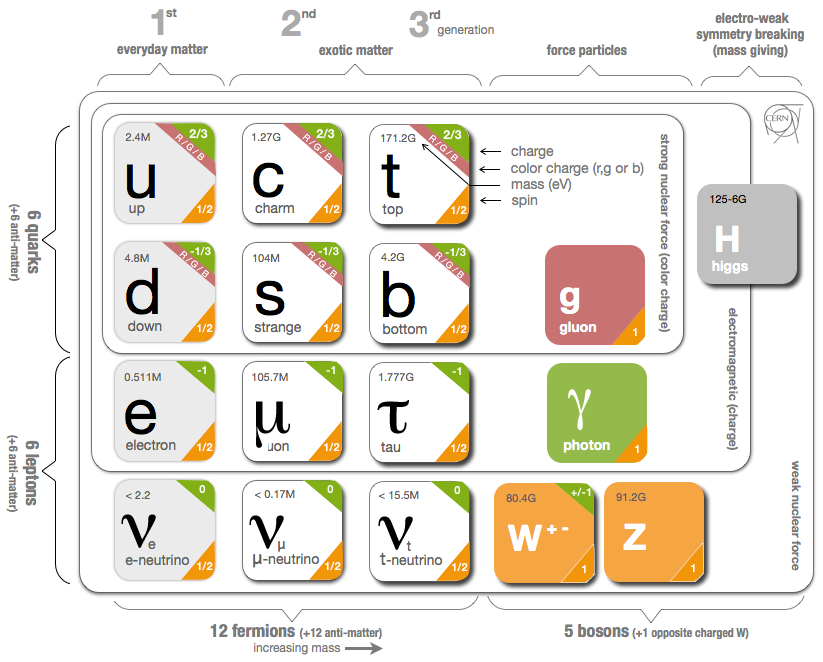
\includegraphics[width = 0.8 \textwidth]{img/I-1/sm-particles.png}
		\caption{Overview of the elementary particles as described by the standard model. Everyday matter is composed of the first generation of quarks and leptons to which two generations of heavier declinaisions are added. Gauge bosons or force particles are the carriers of the interactions between other particles. The Higgs boson is the manifestation of the mechanism that gives mass to particles [CERN].}
		\label{fig:I-1-sm-particles}
	\end{figure}

  Besides classifying particles, the standard model also provide as strong mathematical model built on top of quantum field theory and gauge invariance. The gauge group of the theory is $ SU(3)_C \otimes SU(2)_L \otimes U(1)_Y $, where $ SU(3)_C $ and $ SU(2)_L \otimes U(1)_Y $ are respectivly the symetry groups of the QCD and EWK sectors. Quarks and leptons are represented as fermionic fields within the Lagrangian of the model while bosons arise from the invariance of the Lagrangian under local gauge transformations. \\

  \section{Gauge Invariance and Gauge Bosons}

    A local transformation of a fermionic field $ \psi $ under a gauge group $ G $  can be written as
    \begin{equation}
      \psi \rightarrow \psi' = \exp\left(- \frac{i}{2} g \alpha^k(x) T^k \right) \psi ,
    \end{equation}
    where $ g $ is the gauge coupling constante, $ \alpha^k(x) $ are the local rotation paramters, and $ T^k $ are the generators of the representation of $ G $. To preserve the invariance of the Lagrangian of a free massless field $ \psi $,
    \begin{equation}
      \mathcal{L} = i \bar{\psi} \gamma^\mu \partial_\mu \psi ,
    \end{equation}
    the partial derivate $ \partial_\mu $ must be rewriten as a covariant derivate
    \begin{equation}
      D_\mu = \partial_\mu - \frac{i g}{2} W^k_\mu T^k ,
    \end{equation}
    where $ W^k_\mu $ are the emerging gauge fields associated to $ G $. The gauge invaratiant Lagrangian thus becomes
    \begin{equation}
      \mathcal{L} = i \bar{\psi} \gamma^\mu D_\mu \psi - \frac{1}{4} W^i_{\mu \nu} W^{i \mu \nu} ,
    \end{equation}
    where $ W^i_{\mu \nu} $ are the field strength tensors of the $ W^i_\mu $ gauge fields given by
    \begin{equation}
      W^i_{\mu \nu} = \partial_\mu W^i_\nu - \partial_\nu W^i_\mu - g \epsilon^{ijk} W^j_\nu W^k_\mu ,
    \end{equation}
    with $ \epsilon^{ijk} $ the totaly antisymetrical tensor. Interaction terms between the fermionic field $ \psi $ and the gauge fields $ W^i_\mu $ as well as self-interacting gauge field terms have emerged from the necessity of the invariance of the theory under local transformations. A new massless gauge boson is associated to each generator of the adjoint representation of the symetry group $ G $.

  \section{Electroweak Theory}

    The gauge group of the EWK sector of the standard model is $ SU(2)_L \otimes U(1)_Y $ for which a transformation of a field $ \psi $ can be written as
    \begin{equation}
      \psi \rightarrow \psi' = \exp\left(- \frac{i}{2} g_W \Lambda^k(x) T^k \right) \exp\left(- \frac{i}{2} g_W' \alpha(x) Y \right) \psi ,
    \end{equation}
    where $ g_W $, $ \Lambda^k(x) $, and $ T^k $ are respectivly the gauge coupling, local rotation parameters, and represenation of the $ SU(2)_L $ weak isospin algebra and $ g_W' $, $ \alpha(x) $, and $ Y $ are their $ U(1)_Y $ hypercharge algebra counterparts. The corresponding covariant derivate is
    \begin{equation}
      D_\mu = \partial_\mu - \frac{i g_W}{2} W^k_\mu T^k - \frac{i g_W'}{2} B_\mu Y ,
    \end{equation}
    where $ W^k_\mu $ and $ B_\mu$ are the emerging gauge fields associated to $ SU(2)_L $ and $ U(1)_Y $. \\

    Each fermion can couple differently to the gauge fields according to the representation of the $ SU(2)_L $ group they are part of. To determine the coupling constants it is important to separate each fermionic field into its left-handed and right-handed components such that
    \begin{equation}
      \psi = \psi_L + \psi_R \equiv \gamma^L \psi + \gamma^R \psi ,
    \end{equation}
    with
    \begin{align}
      \gamma^{L/R} & = \frac{1}{2} \left( 1 \mp \gamma^5 \right) \ \text{and} \\
      \gamma^5 & = i \gamma^0 \gamma^1 \gamma^2 \gamma^3 ,
    \end{align}
    where $ \gamma^\mu $ are the Dirac matrices. It has been showed experimentatly that only left-handed particles interact with the $ SU(2)_L $ group, meaning that right-handed particles are part of the trivial representation of the group while left-handed particles are part of the fundamental representation which generators are given by Pauli's matrices. Particles are thus grouped as follows:
    \begin{itemize}
      \item leptons: $ e_R $, $ \mu_R $, $ \tau_R $, $ \left( \begin{matrix} \nu_e \\ e \end{matrix} \right)_L $, $ \left( \begin{matrix} \nu_\mu \\ \mu \end{matrix} \right)_L $, and $ \left( \begin{matrix} \nu_\tau \\ \tau \end{matrix} \right)_L $ ;
      \item quarks: $ u_R $, $ d_R $, $ c_R $, $ s_R $, $ t_R $, $ b_R $, $ \left( \begin{matrix} u \\ d \end{matrix} \right)_L $, $ \left( \begin{matrix} c \\ s \end{matrix} \right)_L $, and $ \left( \begin{matrix} t \\ b \end{matrix} \right)_L $.
    \end{itemize}
    Note that the right-handed neutrinos are not present as they do not interact with particles and are thus sterile. \\

    To each particle, a weak isospin $ T_3 $ can be associated, corresponding to the Casimir operator of $ SU(2)_L $. Right-handed particles have $ T_3 = 0 $, positive quarks and neutrinos have $ T_3 = \frac{1}{2} $, and negative quarks and charged leptons have $ T_3 = - \frac{1}{2} $. The same can be done for the $ U(1)_Y $ group for which an hypercharge $ Y $ is defined. Through breaking of the symetry as explained in the next section, a new relation can be obtained:
    \begin{equation}
      Q = T_3 + Y ,
    \end{equation}
    where $ Q $ is the electric charge of the particle.

  \section{Electroweak Symetry Breaking}

    The physical fields of the photon $ A_\mu $ and the weak interaction bosons $ W^\pm_\mu $ and $ Z_\mu $ are linear combination of the $ B_\mu $ and $ W^i_\mu $ gauge fields. This is a consequence of the higgs mechanism that gives masses to the $ W^\pm $ and $ Z $ bosons but leaves the photon massless, thus breaking the gauge symetry of EWK under $ SU(2)_L \otimes U(1)_Y $ into a $ U(1)_{em} $ symetry group. \\

    To account for the masses of particles, R. Brout, F. Englert, and P. W. Higgs postulated the existance of a scalar doublet in $ SU(2)_L $ with hypercharge $ Y = \frac{1}{2} $
    \begin{equation}
      \phi = \left( \begin{matrix} \phi^+ \\ \phi^0 \end{matrix} \right)
    \end{equation}
    for which the Lagrangian can be written as
    \begin{equation}
      \mathcal{L} = \left( D_\mu \phi \right)^\dagger \left( D^\mu \phi \right) - V(\phi^\dagger \phi)
    \end{equation}
    with $ D_\mu $ the covariant derivate of the $ SU(2)_L \otimes U(1)_Y $ gauge groupe, and $ V $ the potential of the so called Higgs field. The chosen form of $ V $,
    \begin{equation}
      V(\phi^\dagger \phi) = \lambda \left( \phi^\dagger \phi \right)^2 - \mu^2 \phi^\dagger \phi ,
    \end{equation}
    is where the symetry breaking occurs as the ground state of the system is reached when
    \begin{equation}
      \left| \phi \right| = \sqrt{\frac{\mu^2}{2 \lambda}} = \frac{v}{\sqrt{2}} .
    \end{equation}
    The spountaneous breakdown of the symetry accounts for the creation of three Nambu-Goldstone bosons which give their masses to the three weak interaction bosons, and one new field $ H $, the Higgs field. It can be shown that the masses of these particles are directly proportionnal to $ v $:
    \begin{align}
      m_H & = \sqrt{2 \lambda} v \\
      m_Z & = \frac{1}{2} \sqrt{g_W^2 + g_W^2\text{'}} \\
      m_W & = \frac{1}{2} v g .
    \end{align}
    Giving masses to fermionic fields occurs through coupling to the $ \phi $ doublet which respects the gauge invariance of $ SU(2)_L \otimes U(1)_Y $
    \begin{equation}
      \mathcal{L} = - \lambda \bar{\psi}_L \phi \psi_R + h.c.
    \end{equation} \\

    Requiring that the photon field $ A_\mu $ be massless, a linear combination of the $ B_\mu $ and $ W^i_\mu $ must be done
    \begin{align}
      A_\mu & = W^3_\mu \sin \theta_W + B_\mu \cos \theta_W , \\
      Z_\mu & = W^3_\mu \cos \theta_W - B_\mu \sin \theta_W , \\
      W^\pm_\mu & = \frac{1}{\sqrt{2}} \left( W^1_\mu \mp i W^2_\mu \right) \text{and}
    \end{align}
    with
    \begin{equation}
      \tan \theta_W = \frac{g_W'}{g_W} ,
    \end{equation}
    where $ \theta_W $ is the weak mixing or Weinberg angle. From this transformation, it is easy to compute the coupling strengths of particles to the photon field and more particularly the coupling of the positron to the photon
    \begin{equation}
      e = g_w \sin \theta_W .
    \end{equation}

  \section{Quantum Chromodynamics}

    QCD uses the $ SU(3)_C $ gauge group to describe the behaviour of quarks and gluons, and introduces the notion of colour charge. After the observation of particles composed of three identical quarks in the same spin configuration, a new quantum number had to be introduced in order to obey Pauli's exclusion principle. Through their symetry under the $ SU(3)_C $ group, quarks carry a colour (red, blue, or green) that is changed by the interaction with gluons. However, as given quark configurations are not observed experimentaly, a constraint was added and forced hadrons (quark groupments) to be colorless: compoused of a quark and an antiquark of opposite color, or composed of three quarks of different color. \\

    Quarks are placed in the fundamental representation of the $ SU(3)_C $ group which are triplets of the same quark with the three different colours while leptons are singlets as they do not interact under QCD. The convariant derivate becomes
    \begin{equation}
      D_\mu = \partial_\mu - \frac{i g_S}{2} G^a_\mu \lambda^a
    \end{equation}
    where $ g_S $ is the strong coupling constant, $ G^a $ are the 8 gluon gauge fields, and $ \lambda^a $ are the Gell-Mann matrices. Gluons are massless as they do not interact with the Higgs fields.

  \section{Beyond the Standard Model}
 % T OK
  %   \cleardoublepage
  %
  %   \chapter{The Large Hadron Collider}
\label{chap:I-2-lhc}

	The Large Hadron Collider (LHC) \cite{Evans:2008zzb} is a hadron accelerator and collider installed in a 26.7 km long tunnel beneath the Franco-Swiss border near Geneva, at a depth varying from 170 m below the Jura mountains to 45 m below the Leman lake. The tunnel was built by the European Organization for Nuclear Research (CERN) between 1984 and 1989 to host the former Large Electron Positron collider (LEP). As represented in Figure \ref{fig:I-2-lhc-schematic}, which provides a schematic illustration of the LHC, it is composed of eight arcs, eight straight sections (in between the arcs), and two transfer tunnels which connect the LHC to CERN's main injection complex. From the eight possible collision points located in the straight sections of the tunnel, only four are in use and instrumented with a total of seven particle detectors: ALICE \cite{1748-0221-3-08-S08002}, ATLAS \cite{1748-0221-3-08-S08003}, CMS \cite{1748-0221-3-08-S08004}, LHCb \cite{1748-0221-3-08-S08005}, TOTEM \cite{1748-0221-3-08-S08007}, LHCf \cite{1748-0221-3-08-S08006}, and MoEDAL \cite{Acharya:2014nyr}. \\

	\begin{figure}[b!]
		\centering
		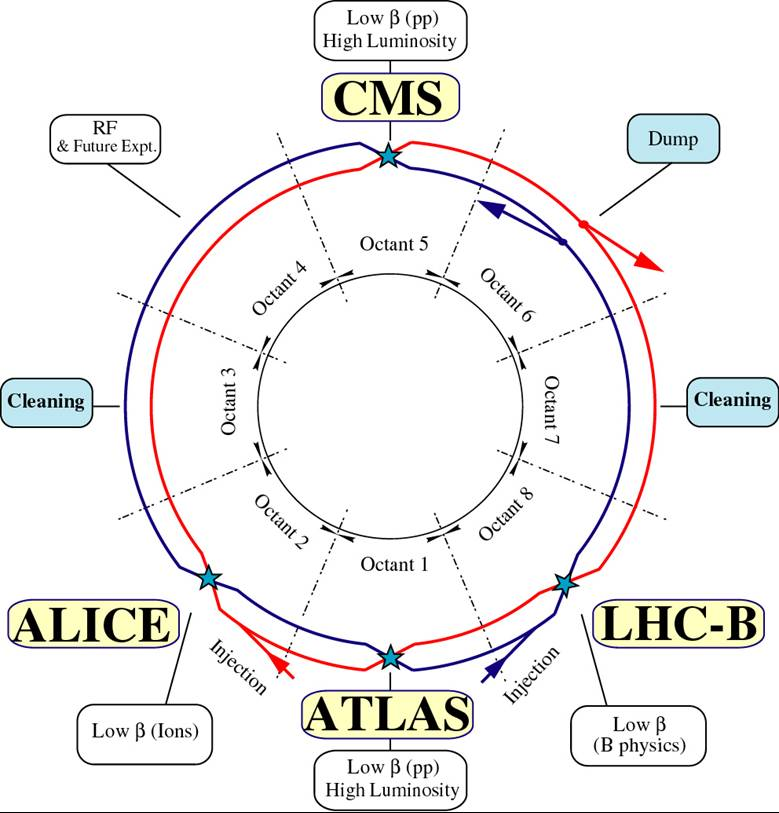
\includegraphics[width=0.7\textwidth]{img/I-2-lhc/lhc.jpg}
		\caption{Schematic representation of the Large Hadron Collider and the four main experiments (ALICE, ATLAS, CMS, and LHCb) that analyze the produced collisions \cite{Evans:2008zzb}.}
		\label{fig:I-2-lhc-schematic}
	\end{figure}

  The construction of the LHC, for which the concept dates back to 1984, was approved by the CERN Council in December 1994 and started in 1998 with the excavation of the caverns that would hold the experimentation sites. In 2003, the first section of the accelerator was assembled inside the tunnel marking the start of the installation phase of the LHC and its detectors, which would span until 2008. On September 10th 2008, the first beam of protons was circulated inside the LHC only to reveal a major technical issue with the superconducting magnets which halted the machine for nearly a year. In November 2009, reparation works were finished just in time for the LHC to produce its first collisions at 2.36 TeV before a Year-End Technical Stop (YETS), a yearly technical stop during which maintenance is performed on the machine. In February 2010, the LHC restarted with a physics program with collisions at 7 TeV that lasted until February 2013. At that time, the LHC stopped for two years during a Long Shutdown (LS) in order to perform upgrades to prepare it to run at 14 TeV. On June 3rd 2015, the LHC restarted and set a new record with an energy in the center of mass reference frame of 13 TeV.

  \section{The Injection Complex}

    The particles that enter the LHC are first created and accelerated by the injection complex of CERN which network of accelerators is depicted in Figure \ref{fig:I-2-injection-chain}. Protons are extracted from gaseous hydrogen by means of a duoplasmatron, a device that uses a heated filament cathode in conjunction with electric fields to produce electrons that will ionize and break the H$_2$ gas. The resulting protons have an energy of 100 keV and are injected in the Linac2 linear accelerator. \\

		\begin{figure}[b!]
			\centering
			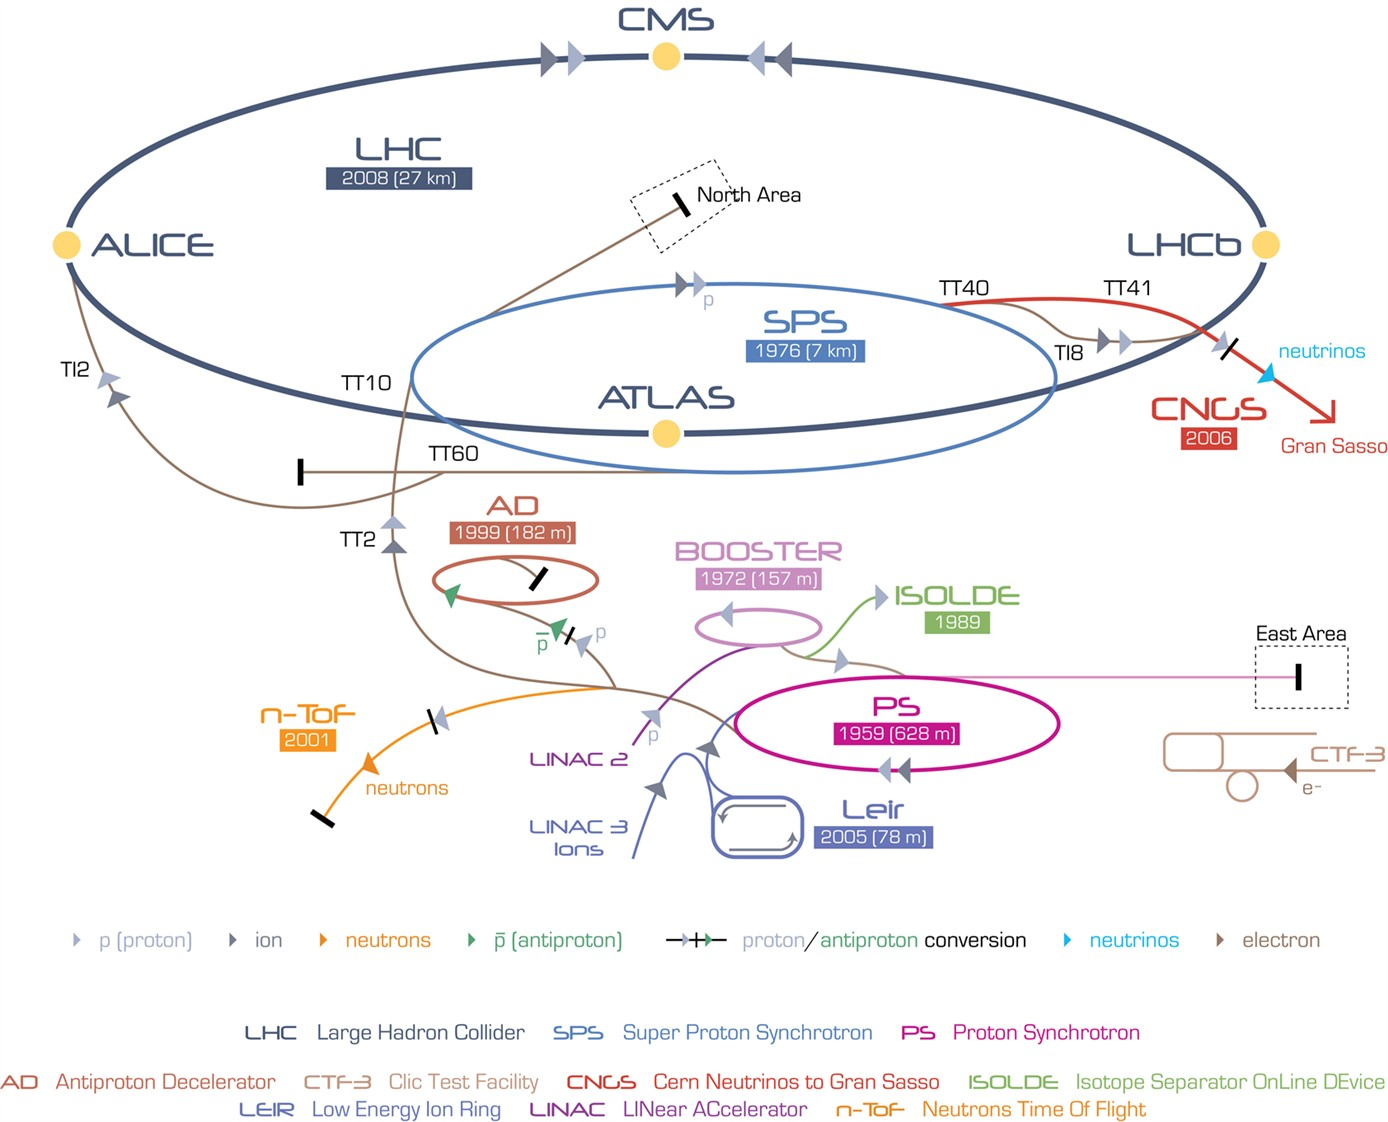
\includegraphics[width=0.9\textwidth]{img/I-2-LHC/injectors.png}
			\caption{Schematic diagram of the injection chain of the LHC composed of multiple smaller accelerators \Cite{TE-EPC-LPC}.}
			\label{fig:I-2-injection-chain}
		\end{figure}

    Linac2 uses radio frequency cavities that produce an electromagnetic field inside the accelerator to transfer energy to the charged particles. The oscillations of the field allow the formation of bunches of particles by regrouping them on the front of the radio wave. The succession of cavities that form Linac2 boosts the incoming protons to an energy of 50 MeV before they enter the Booster. \\

    Following Linac2, three consecutive circular synchrotrons, namely the Proton Synchrotron Booster (Booster), the Proton Synchrotron (PS), and the Super Proton Synchrotron (SPS), accelerate the beams to energies of respectively 1.4 GeV, 25 GeV, and 450 GeV. Each accelerator is composed of electromagnets that bend the trajectory of the beam and boost it further. From the SPS, the beam is injected in the LHC through two transfer tunnels into two rings where particles rotate in opposite directions to be further accelerated until they reach the desired energy. The SPS also provides beam to the North Area where various experiments take place and future technologies can be tested during test beam campaigns, frequently organized by CERN.

  \section{LHC Technical Description}

    Once inside the LHC, particles travel through two beam pipes which are subject to a vacuum of 10$^{-10}$ Torr, representing around 3 000 000 molecules per cm$^3$, which greatly reduces the collisions with the air and allows for greater beam longevity. The beam pipes do not form a perfect circle as they are composed of eight arcs and eight straight sections called insertions. \\

    Each arc contains 154 powerful dipole magnets, represented in Figure \ref{fig:I-2-magnet}, which produce a magnetic field higher than 8 T to bend the beams. The fields are generated by passing high currents through a coil of NbTi superconductor that surrounds the beam pipes cooled by liquid Helium bellow 2 K. The dipoles use a two-in-one design with a common cooling and housing system for the magnets of the two beam pipes which allows to reduce cost and space, and generate a magnetic flux circulating in opposite direction for the two rings. Due to the low temperature at which the magnets operate, the minimum energy deposition left by particles in the coils needed to trigger a quench, a sudden loss of superconductivity, is also decreased. A tight control of the beam structure must thus be enforced. Therefore, 49 quadrupole magnets are installed per section in order to focus the beams and reduce horizontal and vertical spread of the particles. \\

    \begin{figure}[t!]
			\centering
			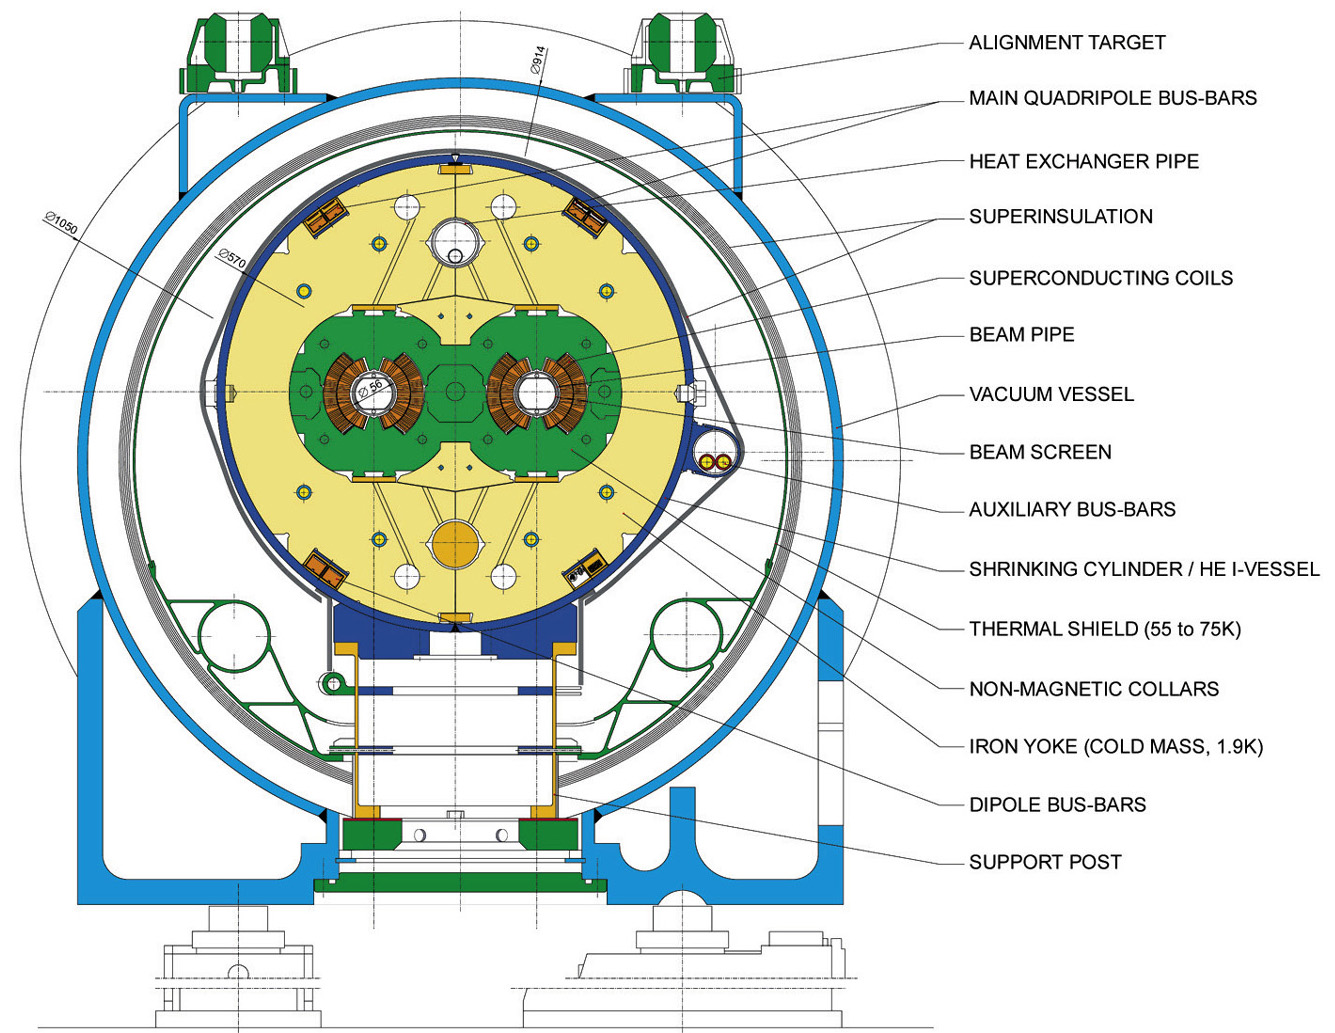
\includegraphics[width=0.75\textwidth]{img/I-2-LHC/magnet.jpg}
			\caption{Cross-section of a cryodipole of the LHC representing the two beam pipes equipped with superconducting NiTb coils surrounded by iron cold mass at 1.9 K \cite{Evans:2008zzb}.}
			\label{fig:I-2-magnet}
		\end{figure}

    The eight straight sections of the LHC have different use cases and designs: four of them are dedicated to the experiments and provide them with collisions, one contains the radio frequency cavities to accelerate the beams, two are used to clean the beam, and one to dump the beam. These functions are fulfilled by using various magnet designs to bend or deflect the beams. From the four collision sites, two also host the beam injection pipes from the SPS into the LHC. The beam cleaning insertions are used to remove particles with out-of-band momentum by scattering them on collimators. When the integrity of the beam is compromised, fast switching magnets activate at the dump insertion in order to quickly extract the particles from the LHC and redirect them to the dump site: an eight meter long graphite composite block that absorbs the energy of the beam.

	\section{Performance Goals}

  	The beams inside the LHC rings are composed of 2 808 bunches each made of approximately 110 billion protons. They are separated by 25 ns which is the time between two consecutive bunch crossing (BX), yielding a collision frequency of 40 MHz. During a collision, only a small fraction of the protons interact depending on various parameters such as the crossing angle of the beams, collimation of the bunches, etc. To quantify this, the notion of luminosity has to be introduced and is directly related to the frequency of apparition of events in a given interaction process
  	\begin{equation}
  		f_{process} = \mathcal{L} \sigma_{process} \ ,
  	\end{equation}
  	where $ f_{process} $ is the number of expected events per second, and $ \sigma_{process} $ is the interaction cross-section of the process. For a circular collider, the instantaneous luminosity is defined as
  	\begin{equation}
  		\mathcal{L} = f \frac{n_1 n_2}{4 \pi \sigma_x \sigma_y},
  	\end{equation}
  	where $ n_i $ is the number of protons or ions per bunch, $ f $ is the frequency of the collisions, and $ \sigma $ is the RMS of the transverse size of the beam in the $x$ and $y$ directions. These parameters change during the operation of the machine as the number of protons per bunch decreases and the bunches spread out. \\

    The instantaneous luminosity can be accumulated over a given period of time in order to obtain the integrated luminosity
  	\begin{equation}
  		L = \int \mathcal{L} \ dt ,
  	\end{equation}
  	which results in the number of events one can expect for a given interaction process
  	\begin{equation}
  		N_{process} = L \sigma_{process} .
  	\end{equation}
    Figure \ref{fig:I-2-luminosity} shows the peak and integrated luminosities delivered by the LHC to its four main experiments during 2015. It can be seen in the picture on the left that the highest instantaneous luminosity reached during that period is on the order of $ 5 \times 10^{33} $ cm$^{-2}$ s$^{-1}$ which is half the nominal luminosity of the current design of the LHC.

		\begin{figure}[t!]
			\centering
			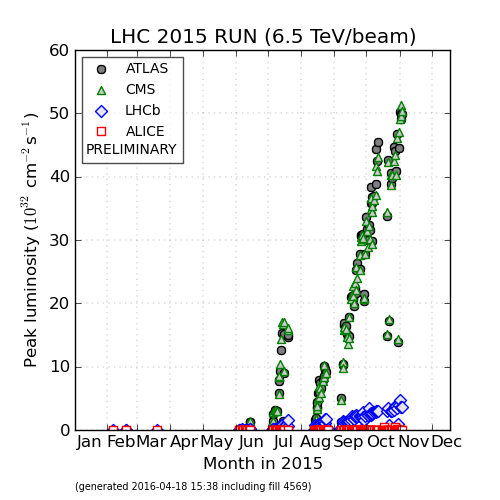
\includegraphics[width=0.49\textwidth]{img/I-2-LHC/luminosity-peak.png}
			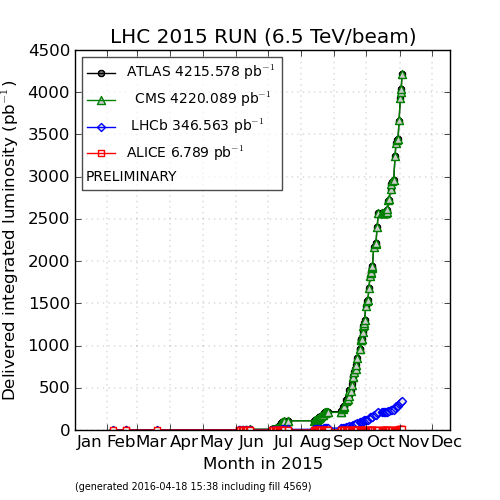
\includegraphics[width=0.49\textwidth]{img/I-2-LHC/luminosity-integrated.png}
			\caption{Monthly evolution of the peak delivered luminosity (left) for the four main experiments of the LHC and the corresponding integrated luminosity (right) \cite{LUMI-PP-LPC}.}
			\label{fig:I-2-luminosity}
		\end{figure}

	\section{Operations and Schedule}

    Over the past years, the LHC has been building up in energy but also in luminosity in order to reach its nominal values of 14 TeV and $ 10^{34} $ cm$^{-2}$ s$^{-1}$. Figure \ref{fig:I-2-future} depicts the schedule of the LHC for the coming years throughout 2037 and the corresponding luminosities: peak on the left axis and integrated on the right axis. It can be seen that several LS are planned in order to upgrade the LHC and allow the experiments to perform maintenance and improvements. A noticeable increase in peak luminosity will occur after LS3 and mark the beginning of the so-called Phase2 operation of the LHC. Such an increase in luminosity will affect the experiments due to the higher number of proton-proton collisions during each BX which will in turn translate to a higher flux of particles in the detectors. Preparing the LHC and the detectors to function at such a high luminosity is a challenge to which physicists and engineers are already providing answers.

    \begin{figure}[t!]
      \centering
      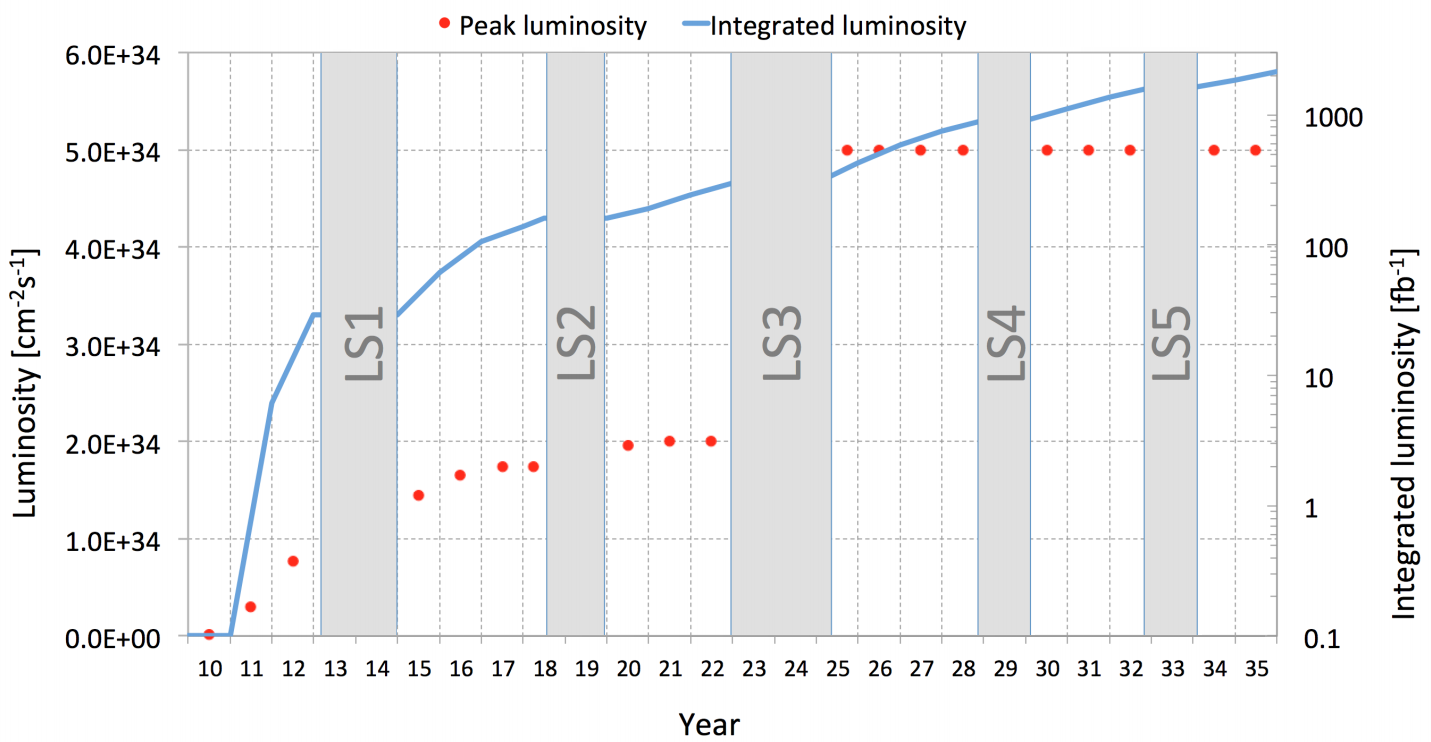
\includegraphics[width=\textwidth]{img/I-2-LHC/lhc-schedule.png}
      \caption{Projected instantaneous and integrated luminosity of the LHC throughout 2037 \cite{HOME-CERN}.}
      \label{fig:I-2-future}
    \end{figure}

  \section{Scientific Motivations}

    The high energy and luminosity at which the LHC operates are the key factors of its success. Reaching new energy levels enables scientists to discover new hidden sectors of physics as new particles can be created through processes that were previously impossible to generate. Moreover, due to the rarity of these events that lie beyond the Standard Model, it is import to accumulate extensive statistics and thus run the machine at high luminosity. \\

    The discovery of the Brout-Englert-Higgs boson is one of the main goals of the LHC which has already been fulfilled. However, the characterization of the particle still requires a great amount of analysis in order to, for example, quantify the coupling constants to fermions or weak bosons. Moreover, it is not excluded that other scalar bosons exist at higher energy as predicted by some theories. In this case, the upgrade of the LHC becomes a necessity to detect the new exotic physics at play. \\

    Not only physics beyond the Standard Model is being explored by the LHC. Measuring the free parameters of the theory and comparing them to theoretical and experimentally obtained values is also an important task which helps validate the models. Running at high luminosity allows the observation of rare processes such as the $ B^0_S $ meson decay, $ \bar{b}s \rightarrow \mu + \bar{\mu} $, which was first observed at the LHC \cite{b0smumu}. \\

    The measurements and observations described above are done by the detectors which are installed on the LHC using the collisions it provides. From the four large experiments the LHC hosts, two of them, namely ATLAS and CMS, are considered to be generalist as they are built to detect a wide range of interactions. ALICE and LHCb on the other hand are respectively optimized to study Pb-Pb interactions at lower energy but which result in a higher density of collisions, and b quark physics to understand the CP violation. The three smaller experiments, namely TOTEM, LHCf, and MoEDAL, use the forward particles that are far away from the interaction point to respectively analyze elastic collisions, simulate cosmic rays, and search for magnetic monopoles.
 % T OK - G OK
  %   \cleardoublepage
  %
  %   \chapter{The Compact Muon Solenoid Experiment}
\label{chap:I-3-cms}

	The Compact Muon Solenoid (CMS) \cite{1748-0221-3-08-S08004} is a multi-purpose particle detector recording the collisions provided by the LHC. It was, along with ATLAS, the first experiment officially approved for the LHC by the CERN research board in January 1997 after a long evaluation process of the letter of intent published four years earlier by the collaboration. The construction of the detector started in 2005, after the excavation works of the cavern finished, and spanned until 2008. Since then, CMS has been proficiently taking and analyzing data, and announced on July 4th 2012 the discovery of the Brout-Englert-Higgs boson, one of the most significant results of the collaboration.

  \section{Overview}

    At nominal energy and luminosity, the LHC produces around 20 proton-proton interactions per BX which results in more than 1 000 particles in the final state. In order to distinguish physical processes with great precision, CMS has to ensure accurate identification and reconstruction of the particles. To this end, the detector was built around four requirements, as stated in \cite{1748-0221-3-08-S08004}:
    \begin{itemize}
      \item Good muon identification and momentum resolution over a wide range of momenta and angles, good dimuon mass resolution ($ \approx $ 1\% at 100 GeV\footnote{The widely used convention that sets $ c = \hbar = 1 $ is used through out this work in order to express energies and masses in electronvolts. A factor of $c^{-1}$ and $c^{-2}$ should respectively be applied to these numbers in order to obtain the values in the international unit system.}), and the ability to determine unambiguously the charge of muons with momentum < 1 TeV;
      \item Good charged-particle momentum resolution and reconstruction efficiency in the inner tracker. Efficient triggering and offline tagging of $ \tau $'s and b-jets, requiring pixel detectors close to the interaction region;
      \item Good electromagnetic energy resolution, good diphoton and dielectron mass resolution ($ \approx $ 1\% at 100 GeV), wide geometric coverage, $ \pi^0 $ rejection, and efficient photon and lepton isolation at high luminosities;
      \item Good missing-transverse-energy and dijet-mass resolution, requiring hadron calorimeters with a large hermetic geometric coverage and with fine lateral segmentation. \\
    \end{itemize}

    \begin{figure}[t!]
      \centering
      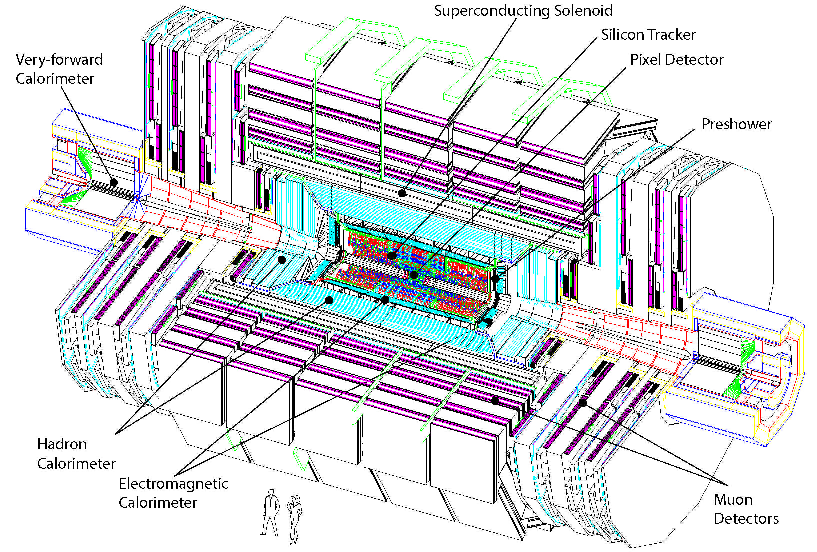
\includegraphics[width=0.9\textwidth]{img/I-3-cms/cms.pdf}
      \caption{The Compact Muon Solenoid detector and its subsystems installed at LHC \cite{1748-0221-3-08-S08004}.}
      \label{fig:I-3-cms-global-view}
    \end{figure}

    These requirements are met through the subdivision of CMS in various detection systems each specialized in the reconstruction of a given type of particles. The overall layout of CMS, shown in Figure \ref{fig:I-3-cms-global-view}, is divided into the barrel and the two endcaps, regions where the detectors are respectively placed parallel and perpendicular to the beam pipe. At the center of the detector, within a radius of 1.25 m around the beam pipe, lies the inner tracking system. Composed of three layers of silicon pixels and ten layers of silicon strips detectors, it is designed to detect the passage of any charged particle with a spatial resolution on the order of 50 $\mu$m. Surrounding the tracking system are the electromagnetic and hadron calorimeters which respectively measure the energy of electrons and photons, and hadrons through the annihilation of the latter within the detectors. These systems are placed inside a superconducting solenoid magnet which produces a strong 3.8 T field that bends charged particles and allows for precise momentum measurements. The obtained resolution on the transverse momentum is so that $\frac{\Delta p_T}{p_T} \approx 1\% $ for 100 GeV muons in the barrel. Outside of the magnet, three different technologies of muon detectors are placed on large iron yokes. \\

    The coordinate system used in CMS has its origin at the nominal interaction point of the beams, the y-axis pointing upwards, the x-axis pointing toward the center of the LHC, and the z-axis directed along the beam direction. The polar coordinates (r, $ \phi $) are defined in the x-y transverse plane and the widely used pseudorapidity $ \eta $ is taken to be
    \begin{equation}
      \eta = - \ln\left( \tan\left( \frac{\theta}{2} \right) \right) ,
    \end{equation}
    where $ \theta $ is the azimuthal angle between the z-axis and the transverse plane.

  \section{The Inner Tracking System}

    The inner tracking system of CMS provides a spatial resolution on the order of 50 $\mu$m with a detection efficiency above 99\% for the passage of charged particles. The proximity of the detectors to the beam pipe yields a high particle density of up to 10$^8$ particles per cm$^2$ at a radius of 4 cm. This justifies the need for a high granularity and fast response time to unambiguously assign particles to the correct collision. This is achieved through a density of up to 4 000 channels per cm$^2$  and a time resolution of 6 ns. However, these features come with an elevated power consumption of a few microwatts per channel which in turn requires a cooling infrastructure to maintain the tracker at a temperature of -20 $^o$C. In order to minimize the material budget of the tracker, a compromise was found to use two technologies: silicon pixels close to the beam pipe to provide a high granularity, and silicon strips further away to minimize the material budget. \\

    The layout of the detectors is shown in Figure \ref{fig:I-3-tracker}. The silicon pixels (PIXEL) are installed on three cylindrical layers in the barrel and two disks in each endcap. These detectors cover an area between radii of 4.4 cm and 10.2 cm and a pseudorapidity $|\eta|$ < 2.5. The silicon strips (TIB, TID, TOB, and TEC) occupy a radial region between 20 cm and 116 cm and are divided in different sectors with a total of 10 layers in the barrel and 12 disks in each endcap. The segmentation into sectors corresponds to the various strip geometries and arrangement. \\

    \begin{figure}[b!]
      \centering
      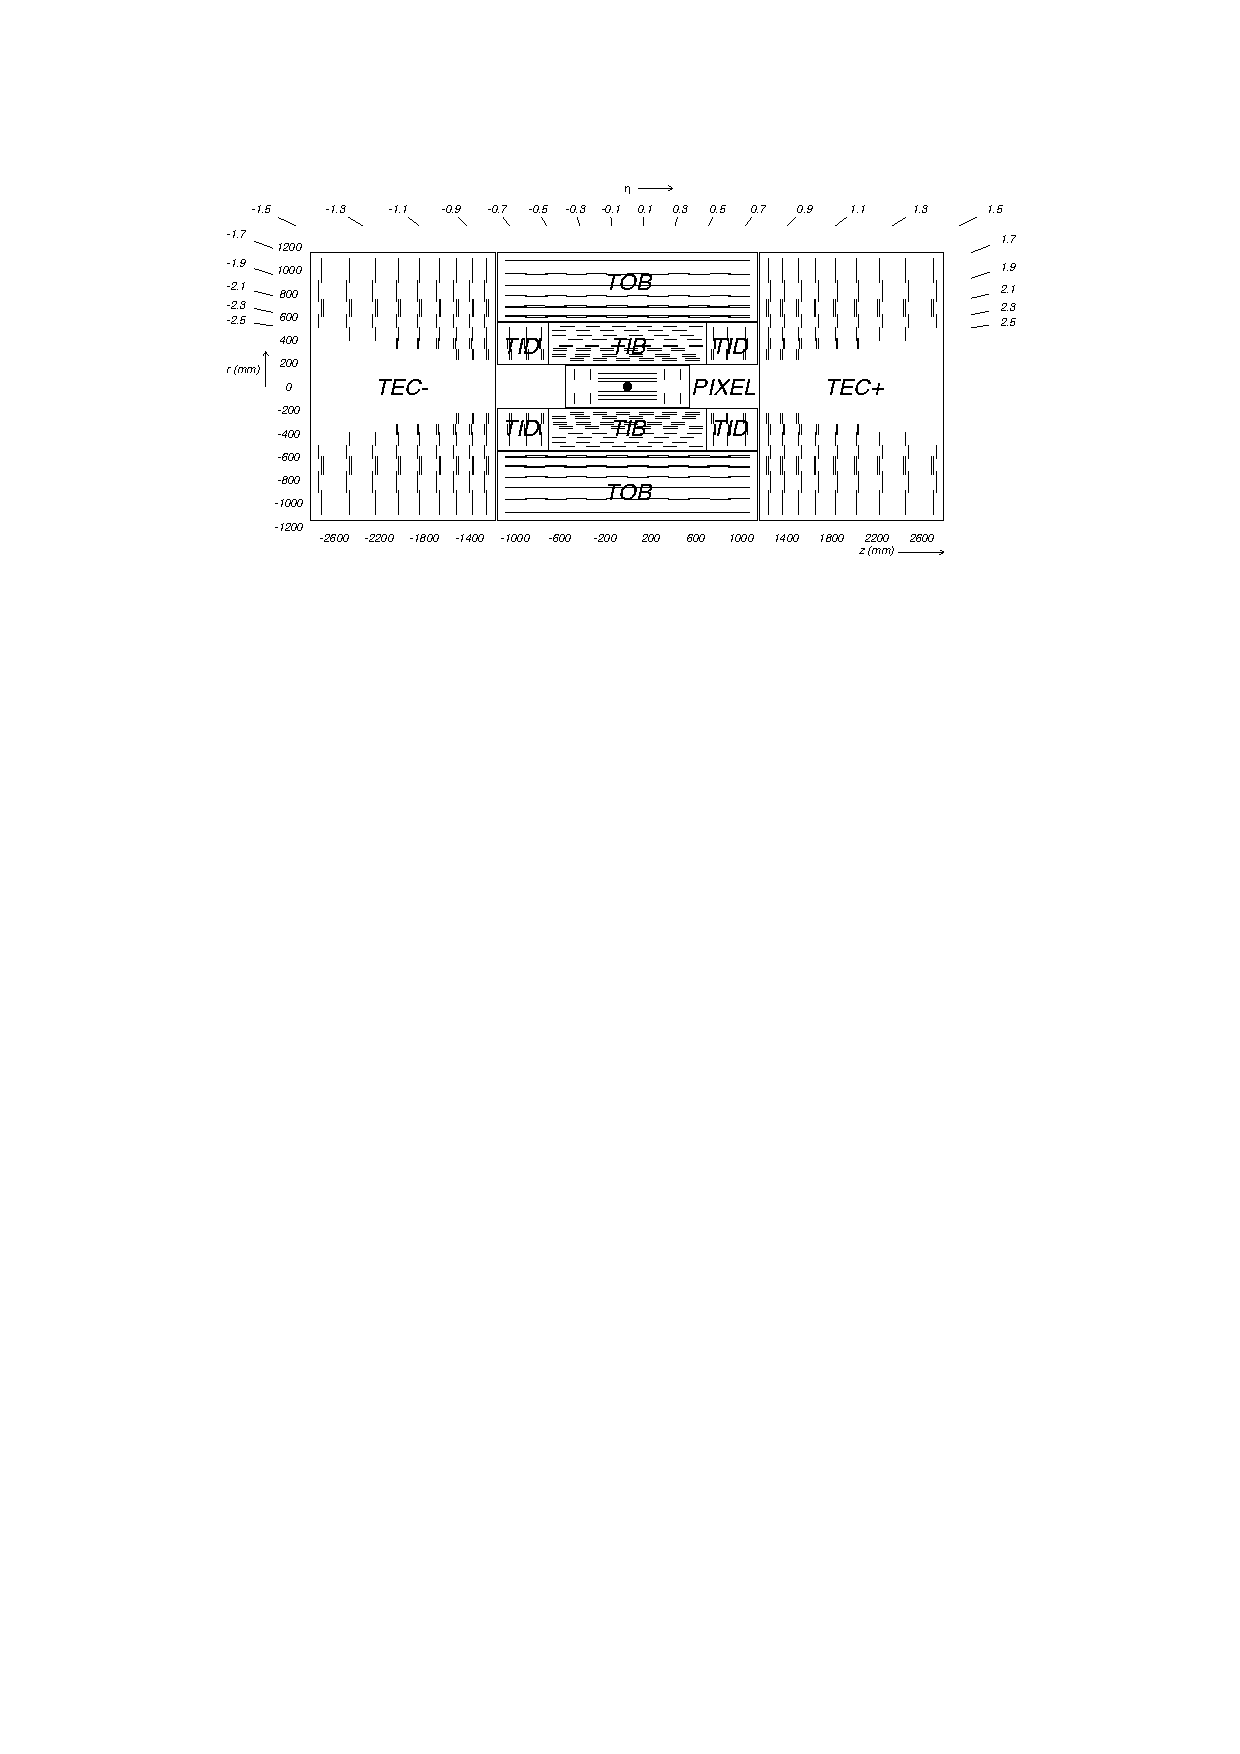
\includegraphics[width=0.86\textwidth]{img/I-3-cms/tracker.pdf}
      \caption{Disposition of the silicon pixels (PIXEL) and strips (TIB, TID, TOB, and TEC) modules inside the tracker of CMS \cite{1748-0221-3-08-S08004}.}
      \label{fig:I-3-tracker}
    \end{figure}

    The barrel pixel tracker contains 768 modules for a total of 48 million pixels. The disks of the endcaps are divided into 24 segments each composed of 7 modules which yield a total number of 672 modules with 18 million pixels for both endcaps. Each pixel is 150 $\mu$m $\times$ 100 $\mu$m in size with a thickness of 260 $\mu$m to 300 $\mu$m resulting in a single point hit resolution of 15 $\mu$m to 20 $\mu$m. \\

    The silicon strip tracker is divided into three subsystems. The Tracker Inner Barrel and Disks (TIB and TID) are composed of 4 layers in the barrel and 3 disks in each endcap, covering a region up to a radius of 55 cm. The strips are 320 $\mu$m thick and run parallel to the beam pipe in the barrel and radially in the disks. The strip pitch is of 80 $\mu$m in the two first layers of the TIB and 120 $\mu$m in the two next ones, resulting in a spatial resolution of respectively 23 $\mu$m and 35 $\mu$m. In the TID, the pitch varies between 100 $\mu$m and 141 $\mu$m. Surrounding the TIB and TID is the Tracker Outer Barrel (TOB) composed of 6 barrel layers of 500 $\mu$m thick strips. It provides a resolution of 53 $\mu$m for the first four layers and 35 $\mu$m for the two last ones. Closing the TOB on both sides are the Tracker EndCaps (TEC) which each holds 9 disks. Additionally, the modules of the two inner layers of the TIB and TOB, the two inner rings of the TID and TEC, and the fifth ring of the TEC are equipped with a second strip detector mounted back-to-back with a stereo angle of 100 mrad and provides a measurement of the second coordinate. \\

    The detection efficiency above 99\% and spatial resolution below 53 $\mu$m of the tracker allows it to achieve a track reconstruction efficiency above 98\% in the $|\eta|$ < 2 region (a dip in efficiency is present at $\eta$ = 0 due to the gap between modules) with a transverse momentum resolution better than 3\% for 100 GeV muons. Figure \ref{fig:I-3-tracker-eff} depicts the track reconstruction efficiency (left) and transverse momentum resolution (right) of the tracker for single muons with transverse momenta of 1, 10 and 100 GeV. \\

    \begin{figure}[b!]
      \centering
      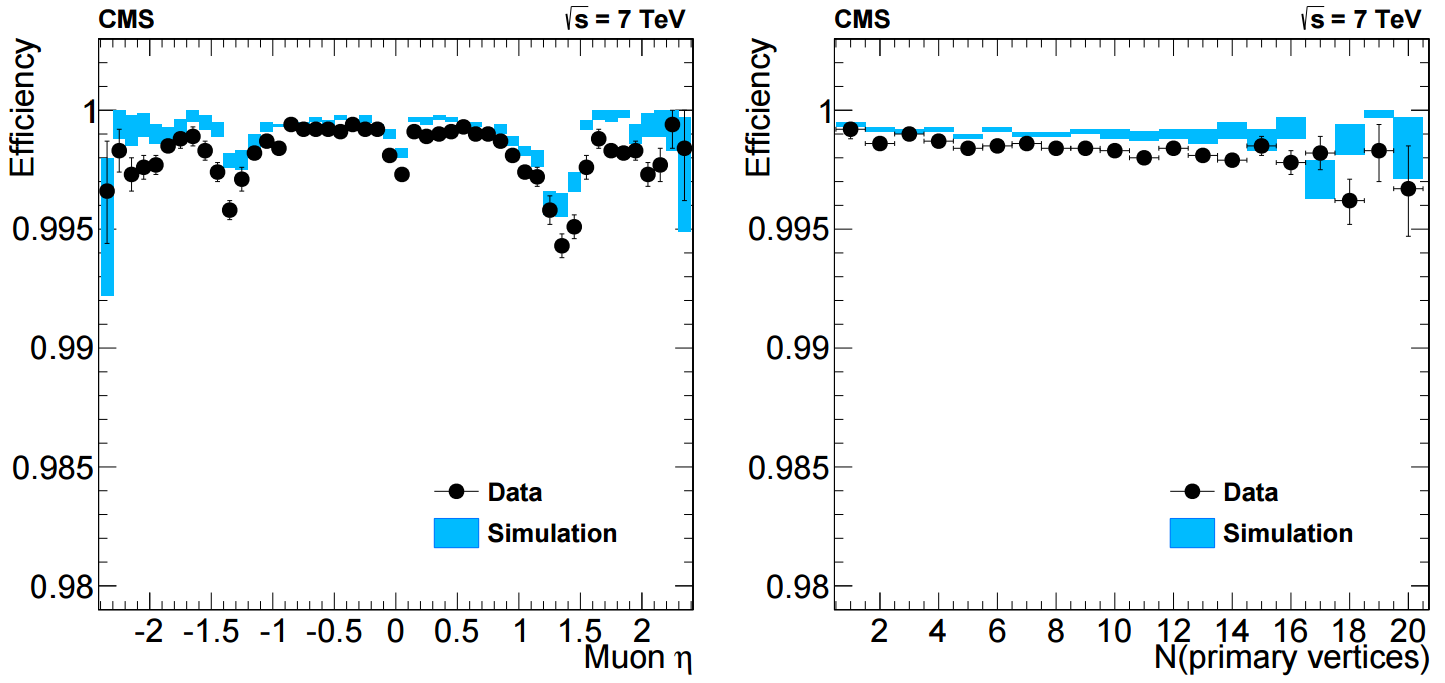
\includegraphics[width=\textwidth]{img/I-3-cms/tracker_efficiency.png}
      \caption{Track reconstruction efficiency (left) and transverse momentum resolution (right) of the tracker for single muons with transverse momenta of 1, 10 and 100 GeV \cite{1748-0221-3-08-S08004}.}
      \label{fig:I-3-tracker-eff}
    \end{figure}

    The resulting material budget of the tracker is shown in Figure \ref{fig:I-3-tracker-material} in which it is expressed in terms of radiation length $X_0$ on the left and hadronic interaction length $\lambda_I$ on the right. From the quantity of material in the tracker, 70\% of the photons materialize into an e$^+$/e$^-$ pair and 5\% of 5 GeV pions interact within its volume.

    \begin{figure}[t!]
      \centering
      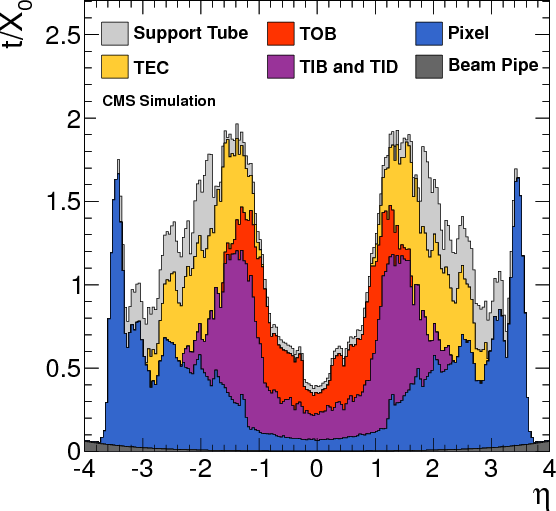
\includegraphics[width=0.49\textwidth]{img/I-3-cms/tracker_budget_e.png}
      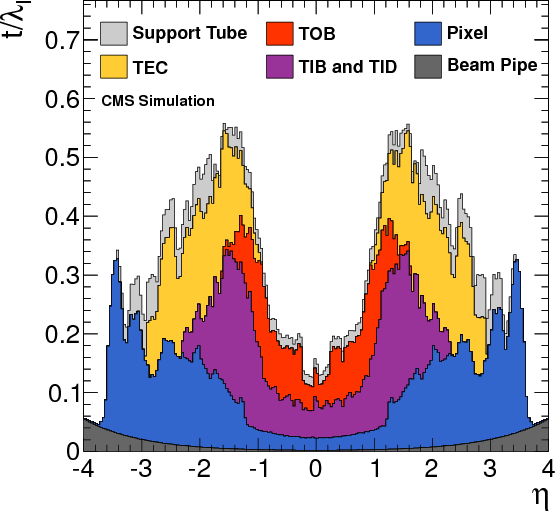
\includegraphics[width=0.49\textwidth]{img/I-3-cms/tracker_budget_h.png}
      \caption{Material budget of the tracker expressed in terms of radiation length $X_0$ on the left and hadronic interaction length $\lambda_I$ on the right \cite{1748-0221-3-08-S08004}.}
      \label{fig:I-3-tracker-material}
    \end{figure}

  \section{The Electromagnetic Calorimeter}

    The Electromagnetic Calorimeter (ECAL) of CMS has been designed to provide an energy resolution for electrons and photons of the order of 1\% for 100 GeV. It is composed of lead tungsten (PbWO$_4$) crystals that act as homogeneous calorimeters: they both initiate the particle cascades and provide the proportional response to the energy deposition. The barrel counts 61 200 crystals and is closed by 7 324 crystals in each endcap. Additionally, a silicon preshower detector is installed in front of the crystals in the endcaps to improve the detection of collimated particles. \\

    The structure of the ECAL is shown in Figure \ref{fig:I-3-ecal}. In the barrel, the ECAL covers a pseudorapidity range $ | \eta | $ < 1.479 and is divided in 360 sections in $ \phi $ and 170 in $ \eta $. The cross section of the crystals varies between 22 mm $ \times $ 22 mm to 26 mm $ \times $ 26 mm for a length of 230 mm corresponding to 25.8 radiation lengths. An alveolar structure maintains crystals together in submodules which are grouped into modules of 400 to 500 crystals further assembled in supermodules containing 1700 crystals in total. In the endcaps, modules cover a pseudorapidity of 1.479 < $ | \eta | $ < 3.0 with each crystal having a front cross-section of 28.62 mm $ \times $ 28.62 mm and a length of 220 mm. These are grouped in units of 5 $ \times $ 5 crystals called supercrystals further inserted in one of the two \emph{Dees} that compose an endcap and maintains the ECAL in place. The preshower uses lead radiators to initiate the avalanche that will be detected by silicon strips to measure the deposited energy and the avalanche profile. Each sensitive module has an active area of 61 mm $\times$ 61 mm divided among 32 strips. The preshower is installed in the 1.653 < $ | \eta | $ < 2.6 pseudorapidity region. \\

    \begin{figure}[t!]
      \centering
      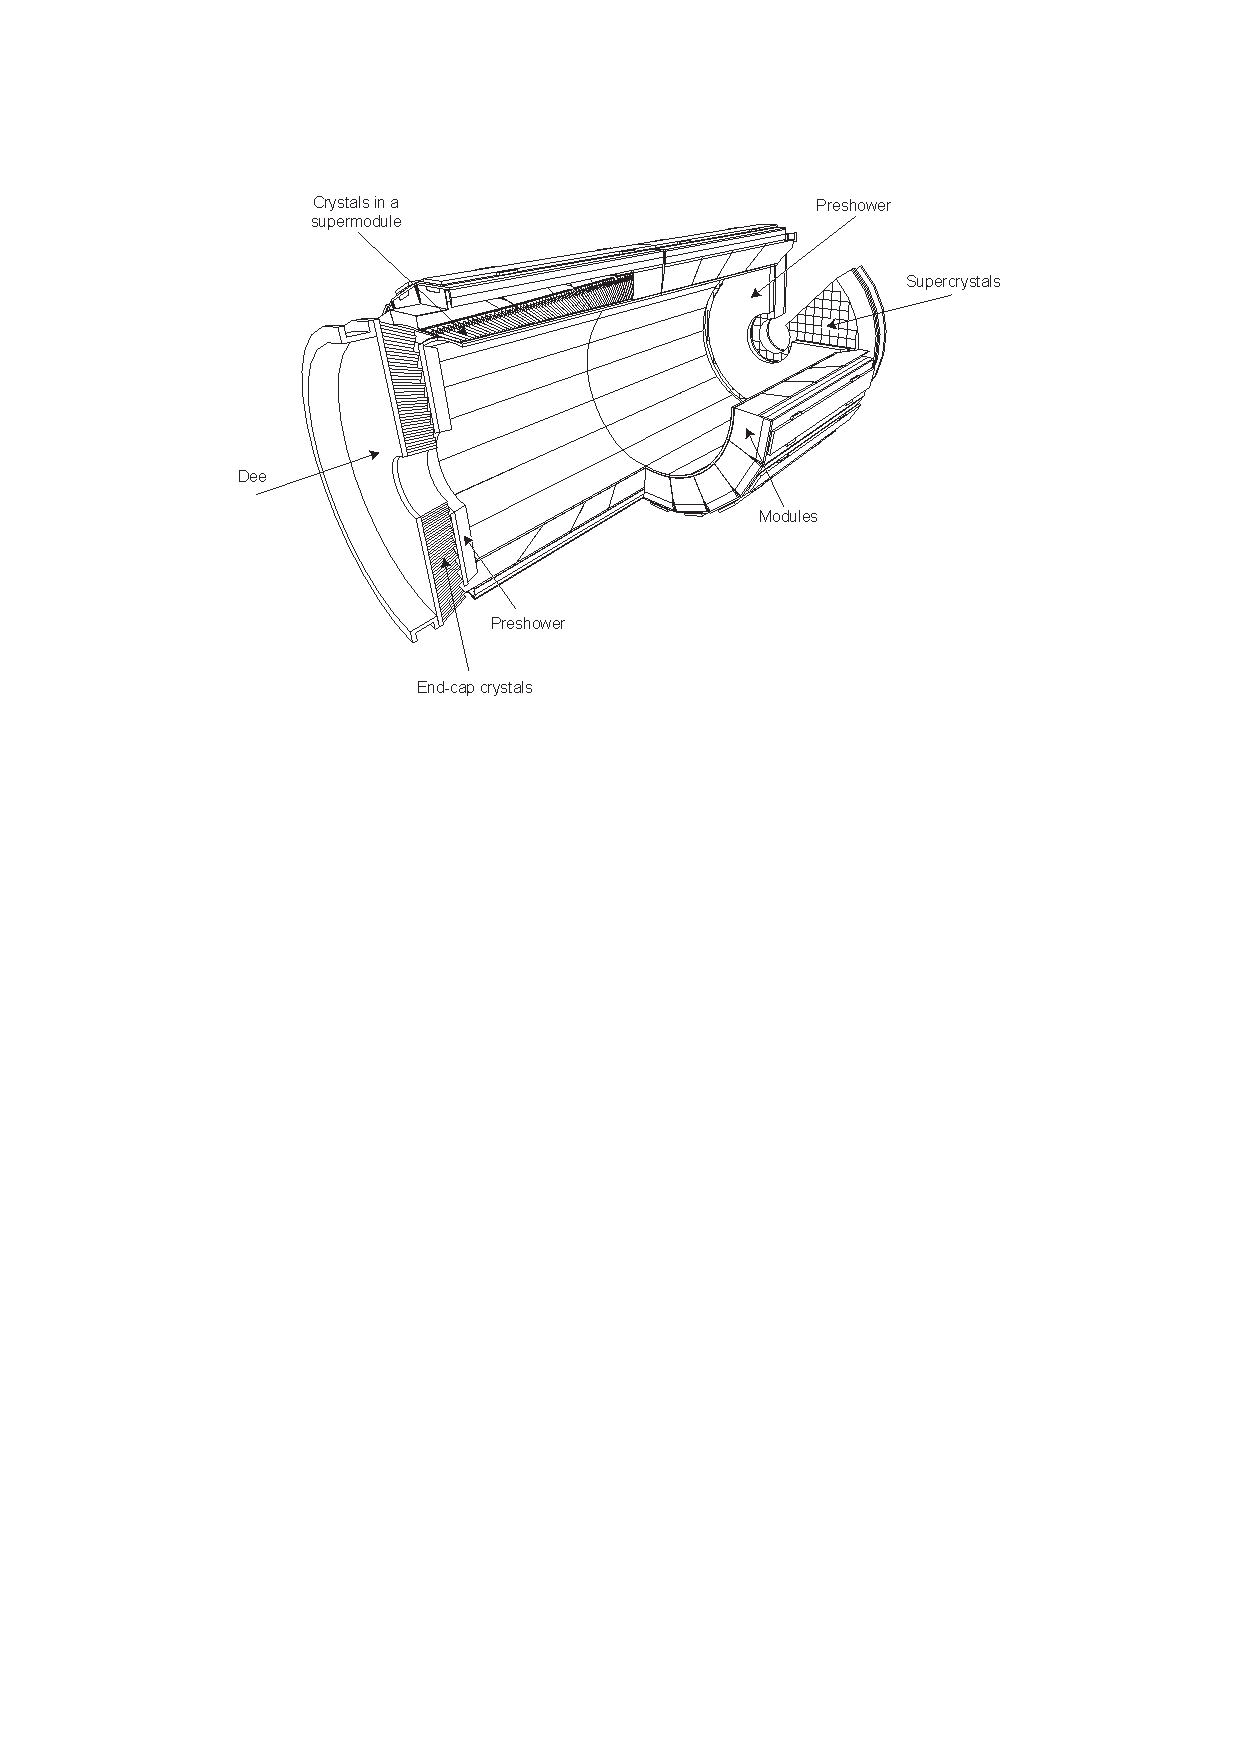
\includegraphics[width=0.7\textwidth]{img/I-3-cms/ecal.pdf}
      \caption{Layout of the ECAL showing the disposition of the crystals, modules, supermodules, and preshower \cite{1748-0221-3-08-S08004}.}
      \label{fig:I-3-ecal}
    \end{figure}

    The energy resolution of the ECAL for particles with energy bellow 500 GeV is parametrized by the following equation:
    \begin{equation}
      \left( \frac{\sigma}{E[GeV]} \right)^2 = \left( \frac{S}{\sqrt{E[GeV]}} \right)^2 + \left( \frac{N}{E[GeV]} \right)^2 + C^2
    \end{equation}
    where $ S $ is the stochastic term, $ N $ the noise term, and $ C $ the constant term. The main contributions to the stochastic term are related to fluctuations in the lateral shower containment, photostatistics contributions, and fluctuations in the energy deposition inside the preshower radiators compared to what is measured by the silicon detector. The noise term includes noise from the electronics, the digitization, and pile-up. Finally, the constant term accounts for non-uniformities in the crystals, calibration errors, and leakage of energy from the back of the crystals. From test beams, the values of $ S $, $ N $, and $ E $, were found to be so that: \\
    \begin{equation}
      \left( \frac{\sigma}{E[GeV]} \right)^2 = \left( \frac{2.8\%}{\sqrt{E[GeV]}} \right)^2 + \left( \frac{0.12}{E[GeV]} \right)^2 + (0.30\%)^2
    \end{equation}

  \section{The Hadron Calorimeter}

    The Hadron Calorimeter (HCAL) provides a measurement of the energy of the hadrons. It is divided into a barrel region (HB), two endcaps regions (HE), and an outer calorimeter (HO) placed right outside the magnet as represented in Figure \ref{fig:I-3-hcal}. The HB sits between the ECAL and the magnet at radii of 1.77 m and 2.95 m respectively, which limits the amount of material and thus absorption lengths that can be used, justifying the need for the HO to catch the tail of the cascades. An additional forward calorimeter (HF) is placed in the very forward region of CMS to analyze particles that are produced or scattered at $ \eta $ > 3. \\

    \begin{figure}[t!]
      \centering
      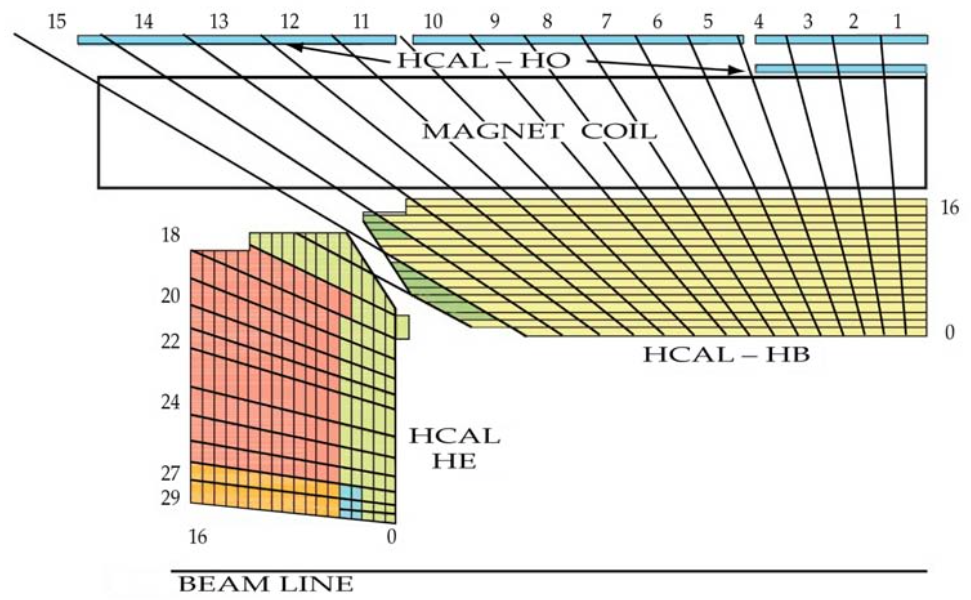
\includegraphics[width=\textwidth]{img/I-3-cms/hcal.png}
      \caption{Longitudinal view of the HCAL showing the disposition of the barrel, endcaps, and outer calorimeters \cite{1748-0221-3-08-S08004}.}
      \label{fig:I-3-hcal}
    \end{figure}

    The HB uses a sampling calorimeter design that consists of a succession of metal sheets positioned parallel to the beam that act as absorber, and plastic scintillators to measure the energy deposition. The absorber is made of a 40-mm-thick front steel panel, followed by eight 50.5-mm-thick brass sheets, six 56.5-mm-thick brass panels, and a 75-mm-thick steel back plate for a total minimum of 5.82 interaction lengths. The scintillators are designed out of 3.7-mm-thick Kuraray SCSN81 plastic and placed after each layer of metal. An additional layer of 9-mm-thick Bicron BC408 is placed in front of the first steel panel in order to sample hadronic showers that might have formed in the ECAL. The scintillator is divided into 16 $ \eta $ and 72 $ \phi $ sectors resulting in a segmentation of $ \Delta \eta \times \Delta \phi $ = 0.087 $ \times $ 0.087. The HE uses 79-mm-thick brass plates spaced by 9 mm gaps in which the plastic Bicron BC408 scintillators are inserted. The segmentation of the HE results in a granularity similar to the HB for $ | \eta | $ < 1.6 and of $ \Delta \eta \times \Delta \phi $ = 0.17 $ \times $ 0.17 for $ | \eta | $ $ \le $ 1.6. In the $ | \eta | $ < 1.3 region, hadron showers are not entirely contained in the HB and HE thus justifying the installation of the HO outside of the magnet to catch the trail of the cascades. This has a significant impact on high energy cascades and the measurement of the missing energy of an event, i.e. the energy carried by non-interacting particles. The HO has a minimum thickness of 1.4 interaction lengths and is segmented in 5 rings further divided into segments. Each segment has a granularity similar to the HB of 0.087 $ \times $ 0.087 in $ \Delta \eta \times \Delta \phi $. Limited by the muon system, the HO has been allocated 40 mm of space, from which 16 mm are used for the scintillators while remaining space is filled with support material. \\

    The energy resolution of the HCAL can be expressed in the same manner as the ECAL, breaking down the result into a stochastic term and a constant term. The obtained resolutions \cite{Baiatian:1049929} are
    \begin{equation}
      \left( \frac{\sigma}{E[GeV]} \right)^2 = \left( \frac{120\%}{\sqrt{E[GeV]}} \right)^2 + (9.5\%)^2
    \end{equation}
    for the HB and HE combined, and
    \begin{equation}
      \left( \frac{\sigma}{E[GeV]} \right)^2 = \left( \frac{280\%}{\sqrt{E[GeV]}} \right)^2 + (11\%)^2
    \end{equation}
    for the HO.

  \section{The Superconducting Magnet}

    The superconducting magnet of CMS measures 6 m of diameter for 12.5 m in length and has been designed to generate a 4 T magnetic field. The return of the magnetic field lines is done through the steel yokes that support the muon chambers of CMS as represented in Figure \ref{fig:I-3-cms-magnet}, in which the amplitude of the magnetic field has been simulated. The magnet is composed of four layers of winded NbTi conductor which offers very low resistance to the nominal 19.14 kA current that is required to generate the field. To reach the superconducting state of the magnet, the latter needs to be cooled down to 1.8 K using liquid Helium. The magnetic field thereby created bends charged particles according to their transverse momentum in the x-y plane
    \begin{equation}
      R = \frac{p_T}{0.3 B} ,
    \end{equation}
    where $ R $ is the curvature radius of the trajectory in the transverse plane, $ p_T $ is the transverse momentum of the particle expressed in GeV, and $ B $ is the intensity of the magnetic field in T.

    \begin{figure}[b!]
      \centering
      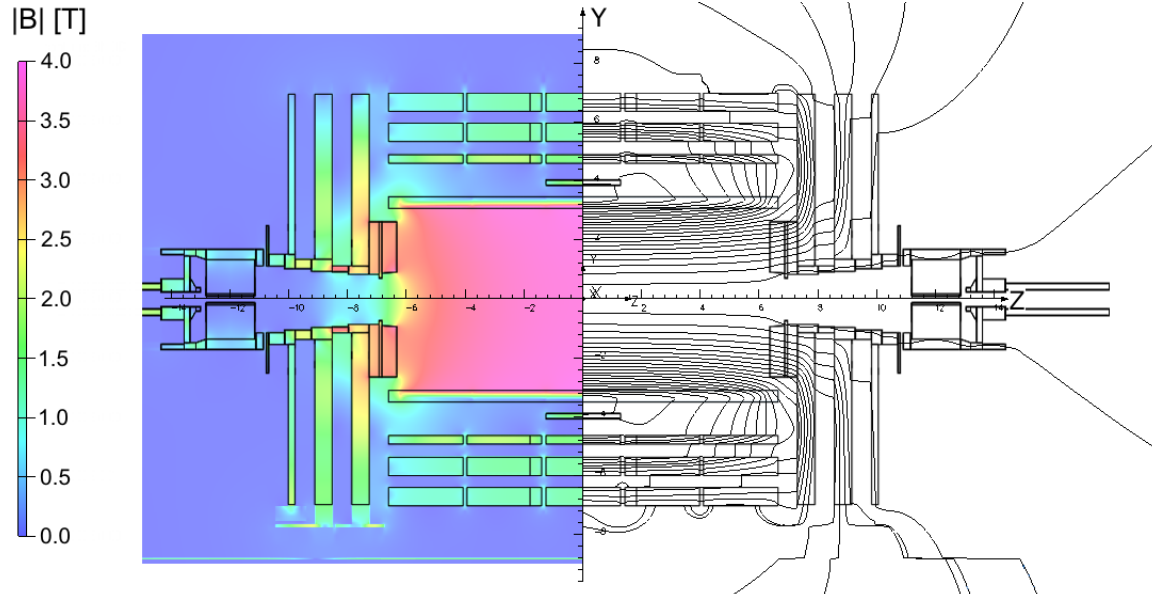
\includegraphics[width=0.8\textwidth]{img/I-3-cms/magnet.png}
      \caption{Representation of the amplitude of the magnetic field and the field lines predicted on a longitudinal section of the CMS detector using simulations \cite{Chatrchyan:2009si}.}
      \label{fig:I-3-cms-magnet}
    \end{figure}

  \section{The Muon System}

    Muons are a recognizable signature from the high background noise produced by the large number of proton-proton interactions. Moreover, they are present in many final states that characterize interesting processes from the Standard Model and beyond. Therefore, providing identification capabilities better than 98\% is essential. CMS is equipped with three different muon detectors that together form the muon spectrometer: Drift Tubes (DTs), Cathode Strip Chambers (CSCs), and Resistive Plate Chambers (RPCs). DTs and CSCs are respectively placed in the barrel and the endcaps while RPCs are installed in both regions, adding redundancy to the system by providing additional measurement points. Figure \ref{fig:I-3-muons} represents a quadrant of CMS highlighting the placement of the various technologies inside the detector. \\

    \begin{figure}[b!]
      \centering
      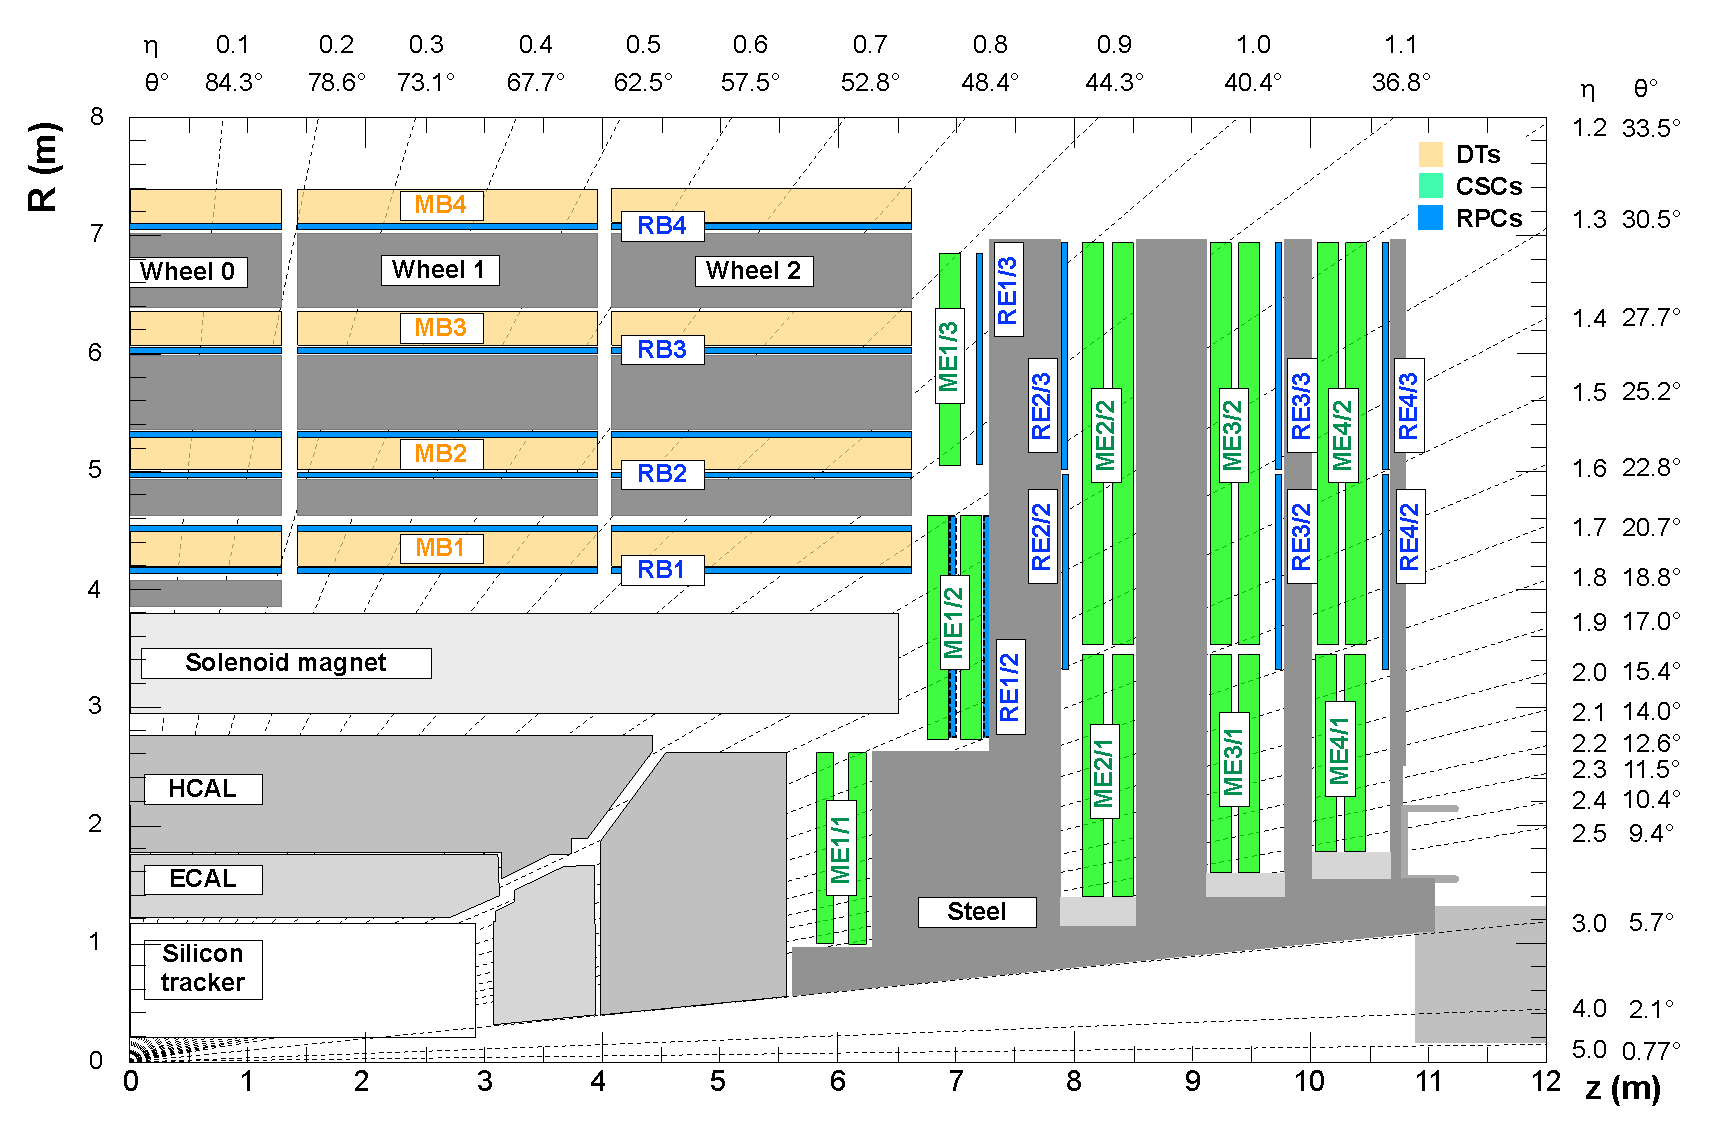
\includegraphics[width=\textwidth]{img/I-3-cms/muons.pdf}
      \caption{Layout of the muon spectrometer of CMS depicting the three gaseous detectors in use: Drift Tubes (DTs) in orange labeled MBx, Cathode Strip Chambers (CSCs) in green labeled MEx/y, and Resistive Plate Chambers (RPCs) in blue labeled RBx and REx/y \cite{1748-0221-3-08-S08004}.}
      \label{fig:I-3-muons}
    \end{figure}

    In the barrel, four cylindrical layers of DTs, numbered MB1 to MB4, cover a pseudorapidity range of $ | \eta | $ < 1.2. The first three layers each contain twelve chambers: eight to measure the r-$\phi$ bending angle and four to measure the z direction. The fourth station solely tracks the r-$\phi$ parameter using eight chambers. \\

    In the endcaps, the CSCs cover a region of 0.9 < $ | \eta | $ < 2.4 and are spread over four disks where detectors are placed perpendicular to the beam pipe. Each disk is further divided into two or three rings numbered MEx/y, where x is the disk number and y is the ring number. CSCs measure both the r-$\phi$ and the $ \eta $ coordinates using respectively cathode strips that run radially and anode wires that run perpendicular to the strips. Each module is composed of 6 layers of CSCs which provide precise background noise rejection and tracking. \\

    Additionally, RPCs are installed along with the DTs and CSCs label RBx and REx/y respectively. In the barrel, two stations of RPCs are installed in RB1 and RB2 while only one station is instrumented in RB3 and RB4. In the endcaps, one module of RPCs equips each of the stations except for the first ring of each disk which has been left empty. This is due to the high rate of particles in the region close to the beam pipe, up to 50 kHz cm$^{-2}$, which is not supported by the RPCs.

    \subsection{Drift Tubes}

      The barrel muon spectrometer consists in 4 cylindrical layers of DT modules: the inner three contain 60 chambers and the outer has 70 for a total of 172 000 sensitive wires. The smallest unit composing the DTs is the drift cell: a 2.4 m long by 42 mm wide tube in which a wire is stretched over the whole length as depicted in Figure \ref{fig:I-3-dt}. Filled with a gas mixture of ArCO$_2$, they provide a measurement of the point of impact of the particle in the direction perpendicular to the wire using the ionization of the gas amplified through the applied high voltage. The small flux of particles in the barrel region of CMS, of the order of 2 Hz cm$^{-2}$, enables the use of these long chambers which limits the number of active channels and thus cost while still providing a spatial resolution in the 80-120 $\mu$m range. Multiple drift cells are combined into layers and four layers are further staggered by half a cell width in order to eliminate dead space and form a super layer (SL). SLs vary in size between 1.9 m in MB1 and 4.1 m in MB4. Each chamber contains two SLs that measure the r-$\phi$ bending angle and one SL that provides a measurement in the z direction. MB4, the fourth station, however does not include the SLs in the z direction. The resolution of a station is on the order of 100 $\mu$m on the position and 1 mrad on the direction of the particle. \\

      \begin{figure}[b!]
        \centering
        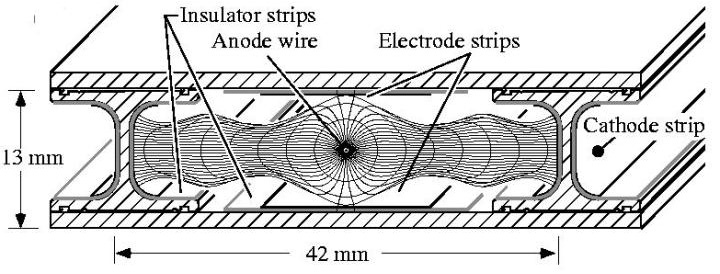
\includegraphics[width=0.8\textwidth]{img/I-3-cms/dt.jpg}
        \caption{Sketch of the drift cells highlighting the electric field lines converging towards the anode wire \cite{1748-0221-3-08-S08004}.}
        \label{fig:I-3-dt}
      \end{figure}

  	\subsection{Cathode Strip Chambers}

      The CSCs are multiwire proportional chambers made of 6 anode wire planes interleaved among 7 cathode strip panels. The largest chambers measure 3.4 m $ \times $ 1.5 m and are installed in the ME2/2, ME3/2, and ME4/2 stations while smaller chambers are mounted in the other stations limited by the steel yoke layout. Taking advantage of the multiple detection layers of the chambers, CSCs can provide a detection efficiency better than 99\%, 75 $\mu$m resolution in the r-$\phi$ coordinate for ME1/1 and ME1/2 and about 150 $\mu$m elsewhere, and a BX assignment efficiency of 99\%. \\

      The structure of the CSCs is shown in Figure \ref{fig:I-3-csc}. Seven 16.2-mm-thick trapezoidal panels made of 12.7-mm-thick polycarbonate core with two 1.6 mm FR4 skins glued on each side are assembled in order to form one chamber. FR4 is a material used to create printed circuit board. On six of the planes, 36 $\mu$m thick copper strips are milled on one side to form the cathode planes. Gap bars are glued to the planes in order to form six gaps of 9.5 mm once the planes are stacked together. About 1000 anode wires are winded around three of the panels in order to form the anode planes. The 50-$\mu$m-thick gold-plated tungsten wires are separated by 3.2 mm and elevated by 4.75 mm with respect to the plane in order to sit in the middle of the gap.

      \begin{figure}[b!]
        \centering
        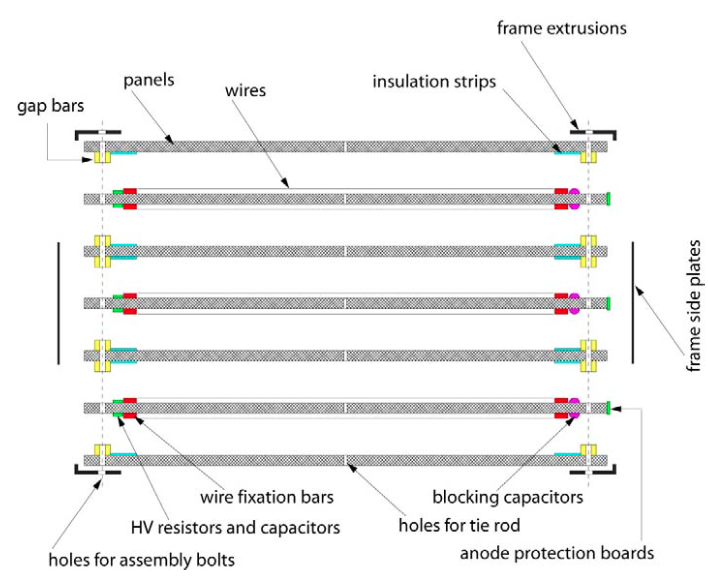
\includegraphics[width=0.85\textwidth]{img/I-3-cms/csc.png}
        \caption{Schematic view of a CSC detailing the different layers that compose it \cite{1748-0221-3-08-S08004}.}
        \label{fig:I-3-csc}
      \end{figure}

  	\subsection{Resistive Plate Chambers}

      RPCs are used for their excellent time resolution of less than 3 ns which allows them to unambiguously assign events to their corresponding BX while also providing a spatial resolution of the order of the centimeter. Each module consists of two gas filled gaps, with a common read-out strip layer in the middle, as depicted in Figure \ref{fig:I-3-rpc}. On each side of the gaps, an insulating backelite panel is covered with a conducting graphite layer on which a high voltage is applied. This layout allows to operate each gap at a lower high voltage and reduce the readout time required, thus improving the time resolution. \\

      \begin{figure}[h!]
        \centering
        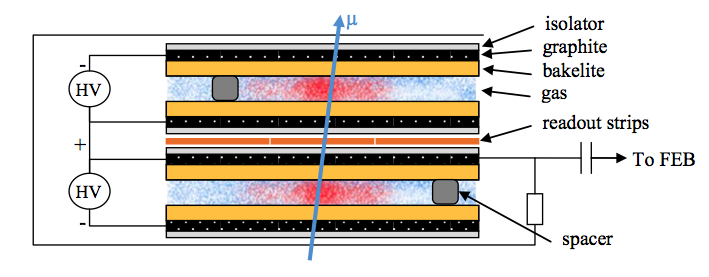
\includegraphics[width=0.7\textwidth]{img/I-3-cms/rpc.png}
        \caption{Diagram of the RPCs double gap layout \cite{1748-0221-3-08-S08004}.}
        \label{fig:I-3-rpc}
      \end{figure}

      In the barrel, RB1 and RB2 each include two RPCs placed on both sides of the DTs. RB3 and RB4 only use one RPC mounted in front of the DTs. In total, 480 chambers are installed, each with a length varying between 2.455 m long and a width between 1.5 m and 2.08 m. In the endcaps, RPCs cover a pseudorapidity range of $ | \eta | $ < 1.6 divided into two rings. Chambers are trapezoidal and cover 20$^o$ in $ \phi $ for the inner ring and 10$^o$ for the outer ring. This setup leaves an empty region between 1.6 < $ | \eta | $ < 2.45 where CSCs are the only detectors providing measurements.

  \section{The Trigger System}

    Every 25 ns and a luminosity of $ 10^{34} $ cm$^{-2}$ s$^{-1}$, approximately 20 proton-proton interactions resulting from the collisions of the LHC occur, yielding more than 1 000 particles in the final state. Each collision generates more than one MB of data which makes it impossible to process and store as is. Therefore, two trigger stages have been implemented to reduce the 40 MHz rate of collisions to 100 kHz at first and 500 Hz afterwards. The Level-1 Trigger (L1 Trigger) consists of custom electronics designed to quickly discriminate between the events. In less than 3.2 $\mu$s the system has to take the decision to forward the event to the next stage or drop it and lose the data. Accepted events are passed to the High Level Trigger (HLT) which runs on a farm of commercial computers. Unlike the L1 Trigger, which due to the small allocated computation time has restricted access to hit information from the detectors, the HLT can use the full granularity of the detector to reconstruct events. \\

    At the L1 Trigger stage, only the information from the HCAL, ECAL, and muon chambers are used as depicted in Figure \ref{fig:I-3-l1}. The energy depositions collected by the HCAL and ECAL are sent to the Calo Trigger Layer 1 which performs data formatting and concentration, and forwards events to the Calo Trigger Layer 2. The latter finds the twelve highest transverse energy jet, tau, and electron/photon candidates and computes global energy sums. \\

    \begin{figure}[t!]
      \centering
      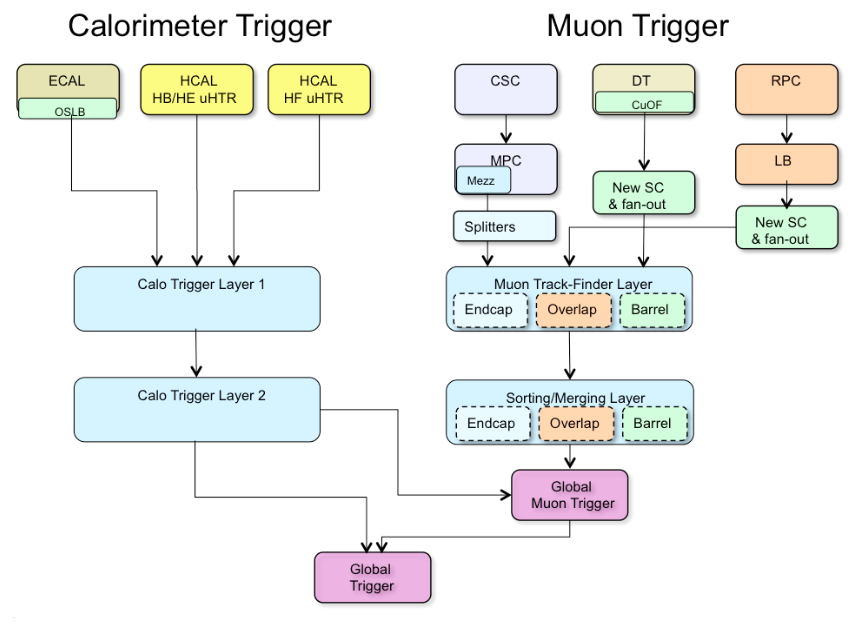
\includegraphics[width=0.8\textwidth]{img/I-3-cms/l1.png}
      \caption{Architecture of the CMS trigger system for both the calorimeter trigger and the muon trigger \cite{Tapper:1556311}.}
      \label{fig:I-3-l1}
    \end{figure}

    The muon trigger is divided into three section: the barrel, the endcaps, and the overlap region where tracks cross both CSCs and DTs. Hits from the different chambers are combined in the Muon Track-Finder layer which uses track extrapolation and pattern recognition algorithms to create tracks. The reconstructed tracks are sent to the sorting/merging layer which selects the best candidates according to quality parameters. The best tracks are sent to the Global Muon Trigger (GMT) which uses information from the calorimeters to compute isolation values for each muon. This combined information is sent to the Global Trigger (GT) along with the data of the calorimeter. \\

    The GT implements a menu of triggers that performs selections on the reconstructed objects such as electrons, photons, or muons and make the decision to accept or reject the events. If an event is accepted, a Level-1 Accept (L1A) is issued and sent to the Trigger Control and Distribution System (TCDS) \cite{Tapper:1556311}. The latter forwards the L1A to all the subsystems according to the readiness of the subdetectors and the data acquisition (DAQ) system. Upon reception of a L1A, the front-end electronics provides the full granularity data to the read-out DAQ which includes the HLT.

  \section{The Data Acquisition System}
  \label{sec:I-3-daq}

    The DAQ system of CMS, shown in Figure \ref{fig:I-3-daq}, reads out the full granularity data of events from more than 650 sources in the whole detector. It is able to handle a data flow of 100 GBytes per second and redirect data to the HLT which reduces the rate of events by a factor of 1 000. \\

      \begin{figure}[h!]
        \centering
        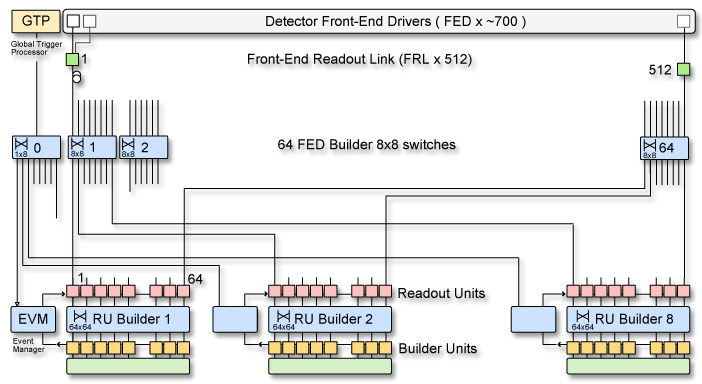
\includegraphics[width=\textwidth]{img/I-3-cms/daq.jpg}
        \caption{Architecture of the DAQ system of CMS \cite{1748-0221-3-08-S08004}.}
        \label{fig:I-3-daq}
      \end{figure}

    For each collision, the front-end electronic modules of the detectors store the full granularity data in buffers and forward reduced information to the trigger system based on which the latter will issue a L1A or not. Upon reception of an L1A from the TCDS, the Front-end drivers (FEDs) will push the full data uplink to the central DAQ system of CMS. To prevent overflow of the buffers during readout, the TCDS system provides back pressure to the FEDs. The event builder then assembles the data of the same L1A of all submodules and provides it to a single filter unit. The latter runs the HLT algorithms on the event and if accepted forwards it for storage.

    \subsection{The Event Builder}

      The event builder is composed of the FED builders and the read-out units (RU) builders. The FED builders are in charge of collecting an average size of 2 kBytes of data from the FEDs and transporting them from the underground cavern to the surface building where 72 super-fragments of roughly 16 kBytes are created. The super-fragments are distributed to the RU-builders on an event by event base, meaning that one unit will handle one event. The fragments are stored in the buffers of the RUs where the RU-builder transfers the event to the event filter.

    \subsection{The Event Filter}

      The role of the event filter is to distribute the events to worker nodes in the processing farm which run offline reconstruction algorithms to process and select events for storage. It is where the HLT is located and is in charge of reducing the 500 kHz rate of data to 100 Hz manageable by the mass storage system. Aside from running reconstruction algorithms, Data Quality Monitoring (DQM) information is also generated for consistency checks. Finally, the selected events are sent for storage to data loggers.

  \section{The Upgrades of CMS}

    Following the maintenance schedule of the LHC, CMS has and will perform upgrades of its detectors to replace aging components and make use of new technologies. Due to the ambient radiation inside the cavern, the aging process of the detectors and their electronics is accelerated. Replacing these elements is thus vital in order to preserve excellent performances. Furthermore, with the increase in luminosity of the LHC, the flux of particles inside CMS will rise, yielding more difficult conditions to detect, identify, and reconstruct events. To solve this challenge, new technologies are being investigated by various collaborations within CMS.
 % T OK
  %   \cleardoublepage
  %
  % \part{The CMS GEM Upgrade Project}
  %
  %   %% Numbers    checked
%% Spelling   checked
%% Acronyms   checked

In the upcoming years, several upgrades of the LHC and its injection chain are planned with the aim of increasing the performance of the machine. The next upgrade, LS2, is currently set to take place in 2019 and will increase the instantaneous luminosity of the LHC to 2 $ \times $ 10$^{34}$ cm$^{-2}$ s$^{-1}$ for the 2020-2022 run. In 2023, the LHC Phase 1 will end with a total integrated luminosity of around 300 fb$^{-1}$ and LS3 will start, allowing to prepare the systems for the so called high-luminosity LHC or LHC Phase 2. The LHC will restart mid-2025 with an instantaneous luminosity of 5 $ \times $ 10$^{34}$ cm$^{-2}$ s$^{-1}$. \\

The muon spectrometer of CMS must be able to cope with the program of the LHC. It was originally designed to be an hermetic and redundant system relying on the DTs, CSCs, and RPCs to provide efficient muon detection, identification, and triggering. The DTs are installed in the barrel and cover a region of |$\eta$| < 1.2, and the CSCs are located in the endcaps between 1.0 < |$\eta$| < 2.4. Additionally, the RPCs provide redundancy in both the barrel and the endcaps but were not instrumented in the |$\eta$| > 1.6 region due to concerns about their tolerance to high fluxes of particles. \\

Besides the lack of redundancy, studies have shown that the triggering efficiency of the muon system of CMS will be drastically affected by the increase in luminosity and reduce the physics performance by limiting the parameter phase-space that can be studied. \\

To tackle these challenges, the CMS GEM collaboration \cite{Colaleo:2021453} will install during LS2 a set of muon detectors that use the Gas Electron Multiplier (GEM) technology in the 1.6 < |$\eta$| < 2.2 region left vacant by the RPCs. The objective is to improve the trigger efficiency in combination with the CSCs. To this end, a new DAQ system has to be designed based on the micro telecommunications computing architecture standard. Small scale systems have been studied during test beam campaigns and four GEM chambers equipped with the full DAQ system will be installed in CMS during the YETS-2016 to perform a so-called slice test. \\

This part focuses on the CMS GEM upgrade project and the developments of the author with respect to the design and characterization of the DAQ system. Chapter \ref{chap:II-1-gem} provides an overview of the GEM technology and the status of the project. It brushes the evolution of the chamber design and the different generations of GEM detectors that have been developed, and covers the performance of the detectors. The architecture of the DAQ system is explained in details in Chapter \ref{chap:II-2-daq} describing each component of the system and their integration in the global CMS DAQ system. Chapter \ref{chap:II-3-test-beam} focuses on the test beam campaigns that took place in November 2014 and 2015 and helped to qualify the system providing results on the chamber performance. Following the test beams, modifications have been made to the electronics in order to prepare for the slice test and the final system which are further detailed. Finally, Chapters \ref{chap:II-4-qualification} and \ref{chap:II-5-irradiation} describe the work performed on the qualification and calibration, and the irradiation tests of the on-detector electronics used in the GEM project. \\

All firmware and software developments, analysis, and results exposed in Chapters \ref{chap:II-3-test-beam}, \ref{chap:II-4-qualification}, and \ref{chap:II-5-irradiation}, have been performed solely by the author unless otherwise specified.
 % T OK
  %   \cleardoublepage
  %
  %   \chapter{Gas Electron Multiplier Detectors}
\label{chap:II-1-gem}

  In 1968, G. Charpak revolutionized the field of tracking detectors by introducing the Multiwire Proportional Chamber (MWPC). MWPCs were more reliable than the existing single-wire gas counters providing a higher sub-mm resolution and rate capabitilies up to fluxes of several MHz cm$^{-2}$. Developments of manufacturing technics and high-density electronics led to a new generation of detectors fulfilling the needs of high-energy physics experimentation. However, their use in high-luminosity experiments revealed some intrensic weaknesses: the mechanical design of the chamber limits the spacial resolution; long ion drift times affect the efficiency of the detector at high fluxes; solid deposits aglomerate on the wires due to aging and induce sparks in the chamber. \\

  Twenty years later, Micro-Strip Gas Counters (MSGCs) were developped using photolithographic processes to engrave anode and cathode strips on an insulating support. Both the position resolution and the rate capability were increase by several orders of magnitude. Unfortunalty, the detectors were prone to the effect of aging and discharges, irremediably damaging the counters. \\

  The relative success of the MSGCs led to the development of Micro-Pattern Gas Detectors (MPGDs) less suseptible to discharges and offering comparable performances. They make use of micro pattern structures to amplify the signal and reduce the probability of sparks inside the chamber. Two technologies have proven to be operationnal: the micro-mesh gaseous structure (MICROMEGAS) and the Gas Electron Multiplier (GEM) \cite{SAULI1997531}. \\

  Already in use in the COMPASS and TOTEM experiments at CERN, GEM detectors have proven to meet the requirements of high-luminosity environments. In 2009, a dedicated R\&D program was launched to study the feasability of the installation of GEMs in the muon spectrometer of CMS to instrument the positions left vacant by RPCs. Seven years later, the so called GE1/1 muon detector upgrade project has been approved by CMS to be installed during LS2.

  \section{Motivations for the GE1/1 Muon Detector Upgrade}

    During LS2 that will take place in 2018-2019, the CMS GEM collaboration \cite{Colaleo:2021453} will install an additional set of muon detectors in CMS in the 1.6 < |$\eta$| < 2.2 region. The so-called GE1/1 detector will be installed near the ME1/1 CSCs station as shown in Figure \ref{fig:II-1-gem-ge11} which highlights the location of the chamber within the muon spectrometer. \\

    \begin{figure}[h!]
      \centering
      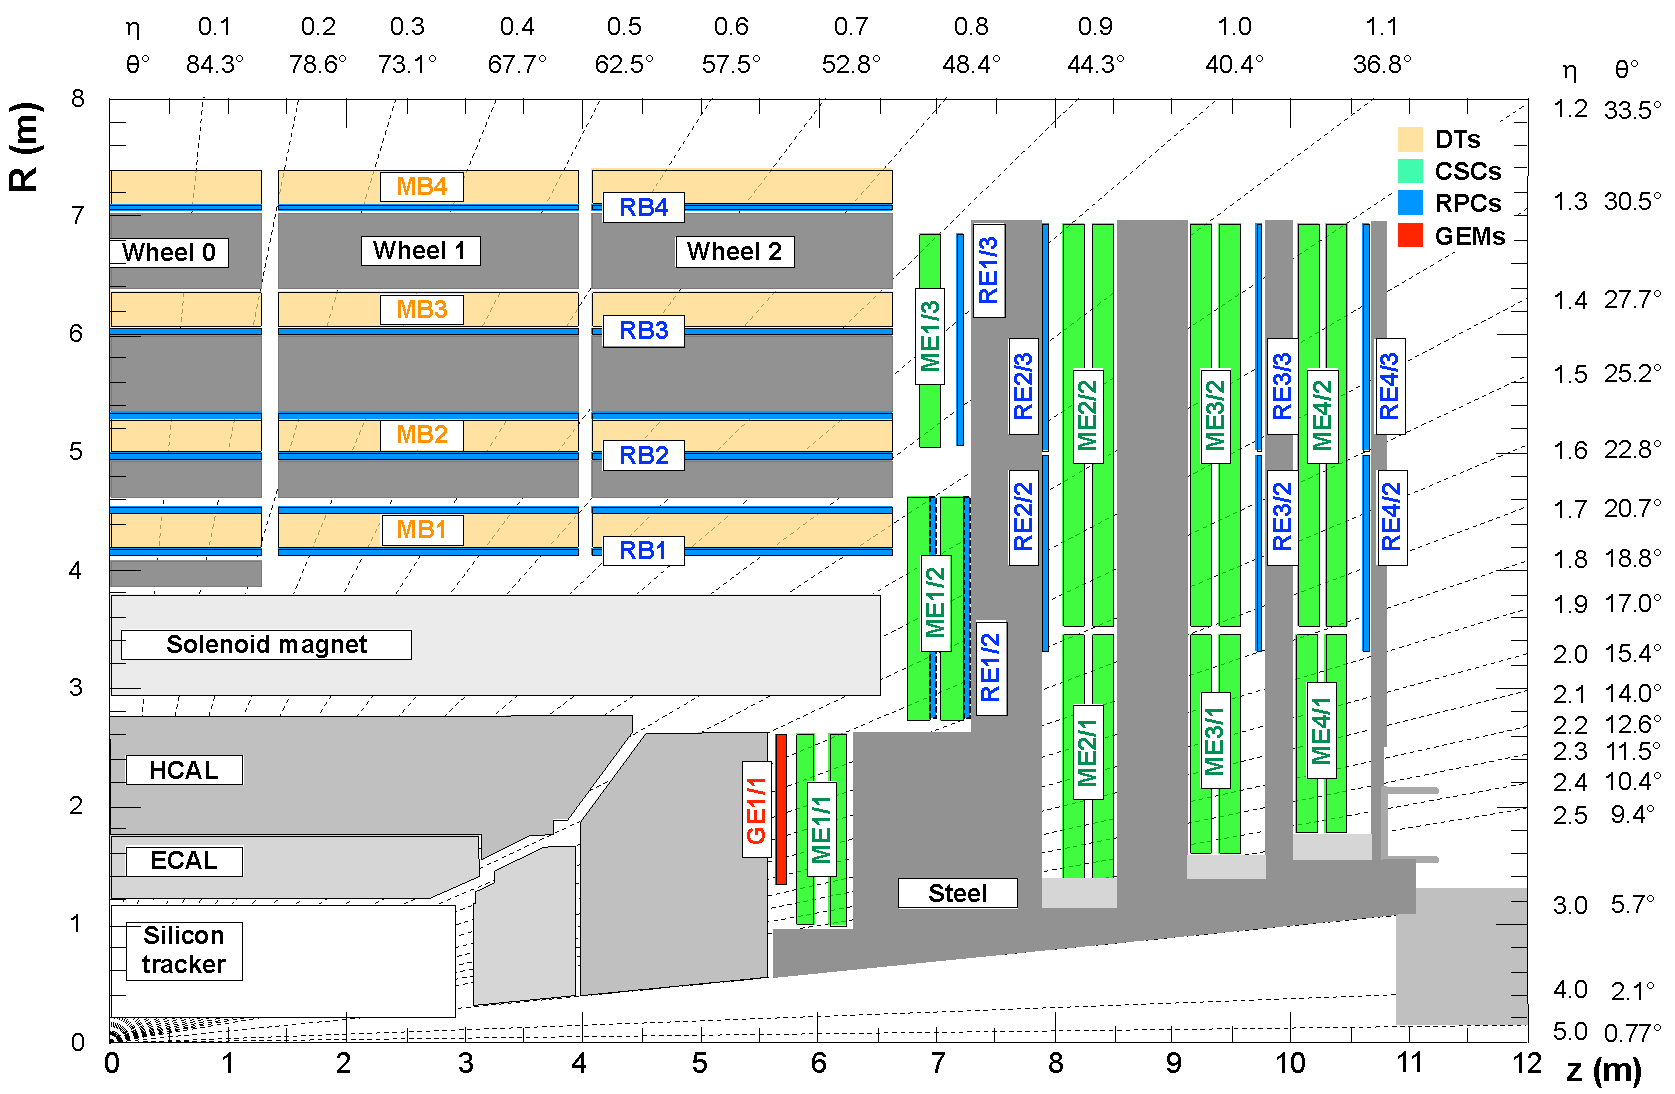
\includegraphics[width=\textwidth]{img/II-1-gem/ge11-quadrant.pdf}
      \caption{Schematic representation of a quadrant of CMS highlighting the location of the GE1/1 detector in red within the muon spectrometer. DTs are represented in yellow, CSCs in green, and RPCs in blue \cite{Colaleo:2021453}.}
      \label{fig:II-1-gem-ge11}
    \end{figure}

    The main motivation for the installation of GE1/1 is the significant impact it has on the triggering system of CMS. Left as is, the performance of the current system would degrade in the coming years with the increase in instantenuous luminosity due to the rate limitations of the ME1/1 station exposed to an intense flux of particles. Muon triggering will in turn suffer a degradation in transverse momentum, p$_T$, resolution. As muon triggers are limited in bandwidth to a fraction of the total allocated bandwidth of the trigger, typically a few kHz, they must set a cut on the minimum p$_T$ of the muons. In the scenario where the muon spectrometer remains unmodified, the threshold would have to be raised to p$_T$ $ \approx $ 30 GeV c$^{-1}$ which would be a considerable drawback in terms of physics analysis. \\

    To prevent the degradation of the trigger system, the GEM collaboration investigated the possibility to use the bending angle of tracks between GE1/1 and ME1/1 to estimate the p$_T$ of muons, which trajectory is curvated by the magnetic field. Figure \ref{fig:II-1-gem-csc-bending} shows on the left the lever arm given by the 20 cm to 46 cm distance between the two detectors. The variation in distance corresponds to "close" and "far" chambers which are staggered in order to allow for some overlap and avoid deadspace. From this, the picture on the right displays the discrimination power between 5 GeV c$^{-1}$ and a 20 GeV c$^{-1}$ muons. \\

    \begin{figure}[h!]
      \centering
      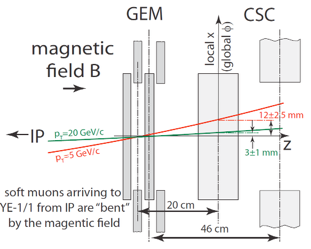
\includegraphics[width=0.45\textwidth]{img/II-1-gem/gem-csc-bending-1.png}
      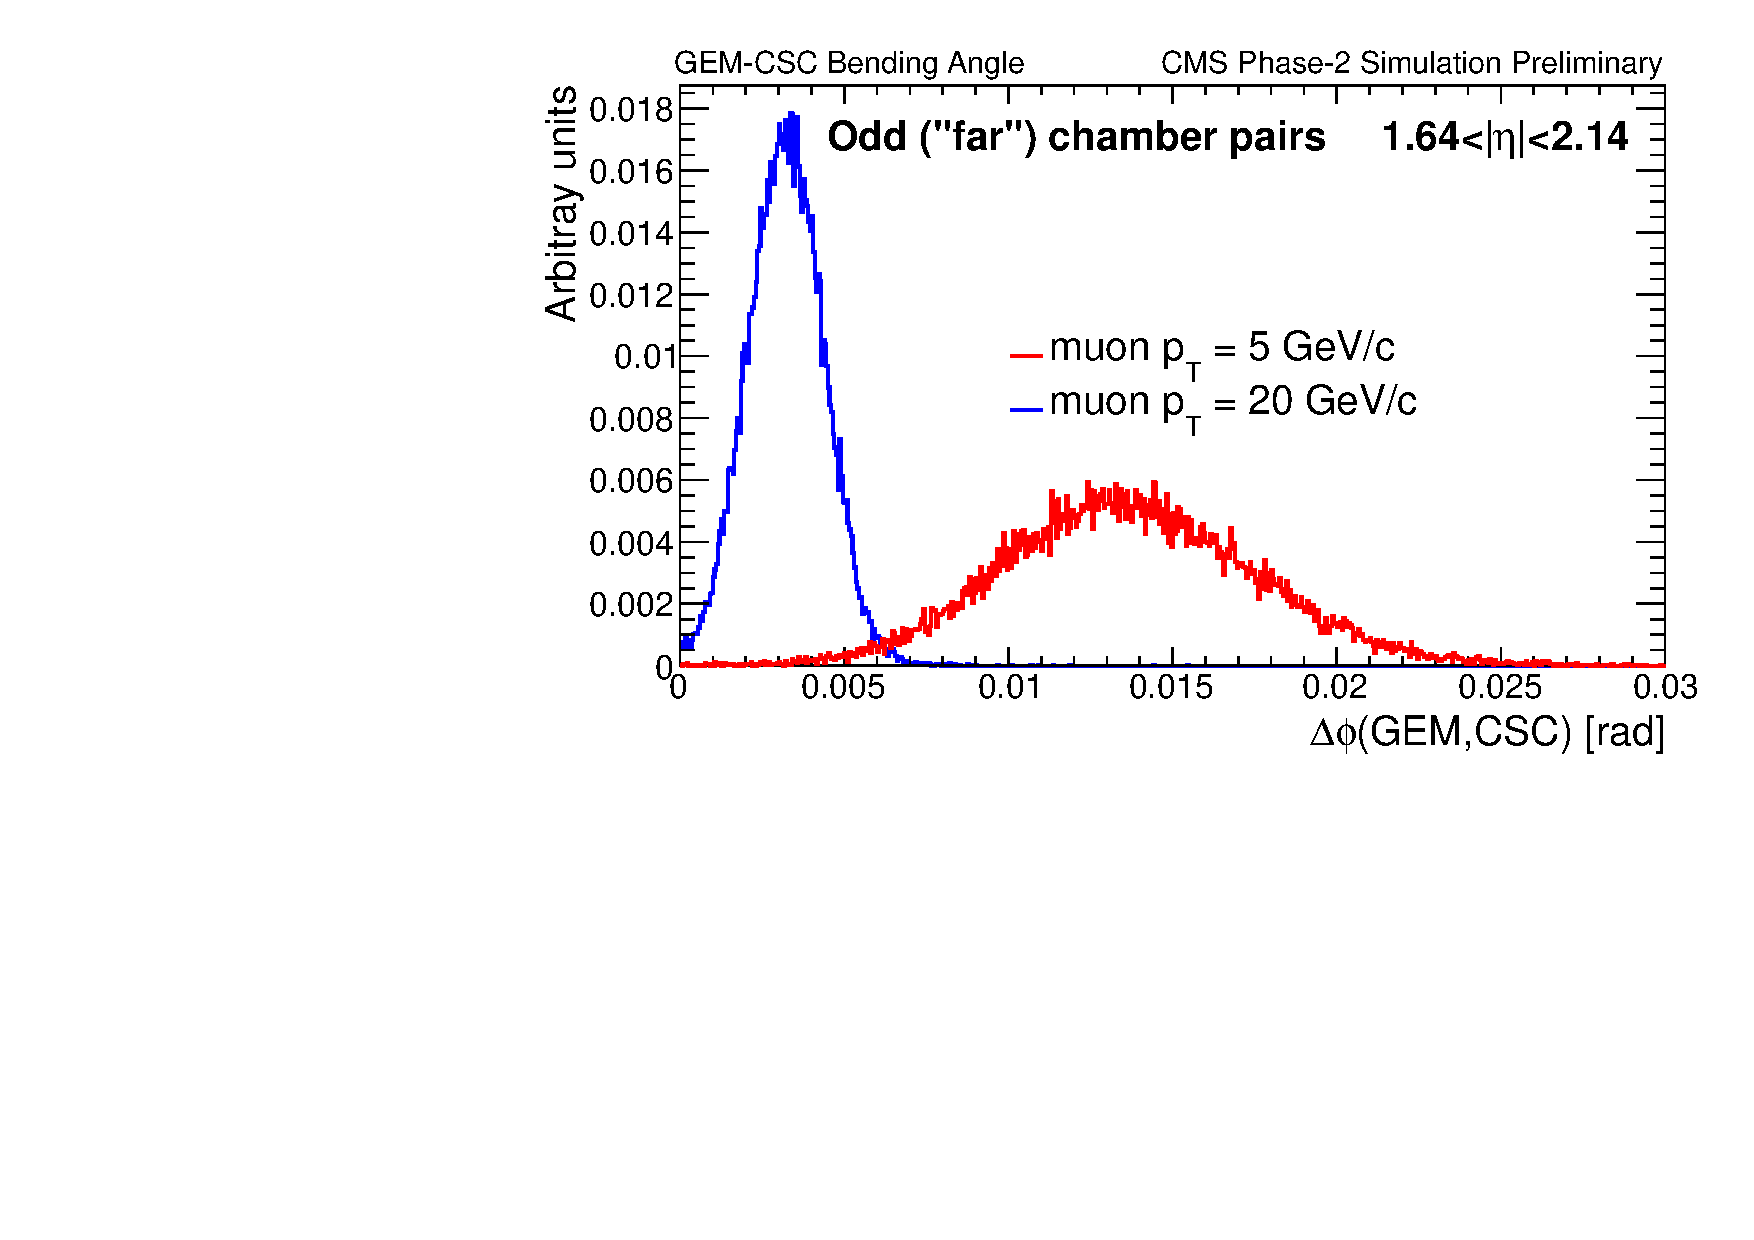
\includegraphics[width=0.53\textwidth]{img/II-1-gem/gem-csc-bending-2.pdf}
      \caption{Left: sketch of a measurement of the bending angle with a pair of a CSC and a GEM chamber, illustrating discrimination between lower and higher momentum muons. Right: $ \Delta \phi = \phi_{GE1/1} - \phi_{ME1/1} $ distribution for 5 GeV and 20 GeV p$_T$ muons demonstrating the discrimination power of the combined GEM-CSC system \cite{Colaleo:2021453}.}
      \label{fig:II-1-gem-csc-bending}
    \end{figure}

    Using these results, a common effort from the GEM and CSC collaboration ensued to integrate the GEM measurments in the CSC trigger system to provide an additionnal layer of information. Using simulations, it has been shown that the efficiency of system increases thus yeilding a lower rate of triggers. These results are shown in Figure \ref{fig:II-1-gem-trigger}. In the left plot, it can be seen that the efficiency of the GEM and CSC combined trigger in blue is superior to the CSC only results in red, recovering the losses occuring at higher rates. In the right plot, it is depicted how the trigger rate of the combined system in blue diminishes by one order of magnitude compared to the current system in red. For a given trigger rate, a smaller muon p$_T$ threshold can be applied due to lower rate of misreconstructed particles, which improves the physics performance of the detectors. \\

    \begin{figure}[h!]
      \centering
      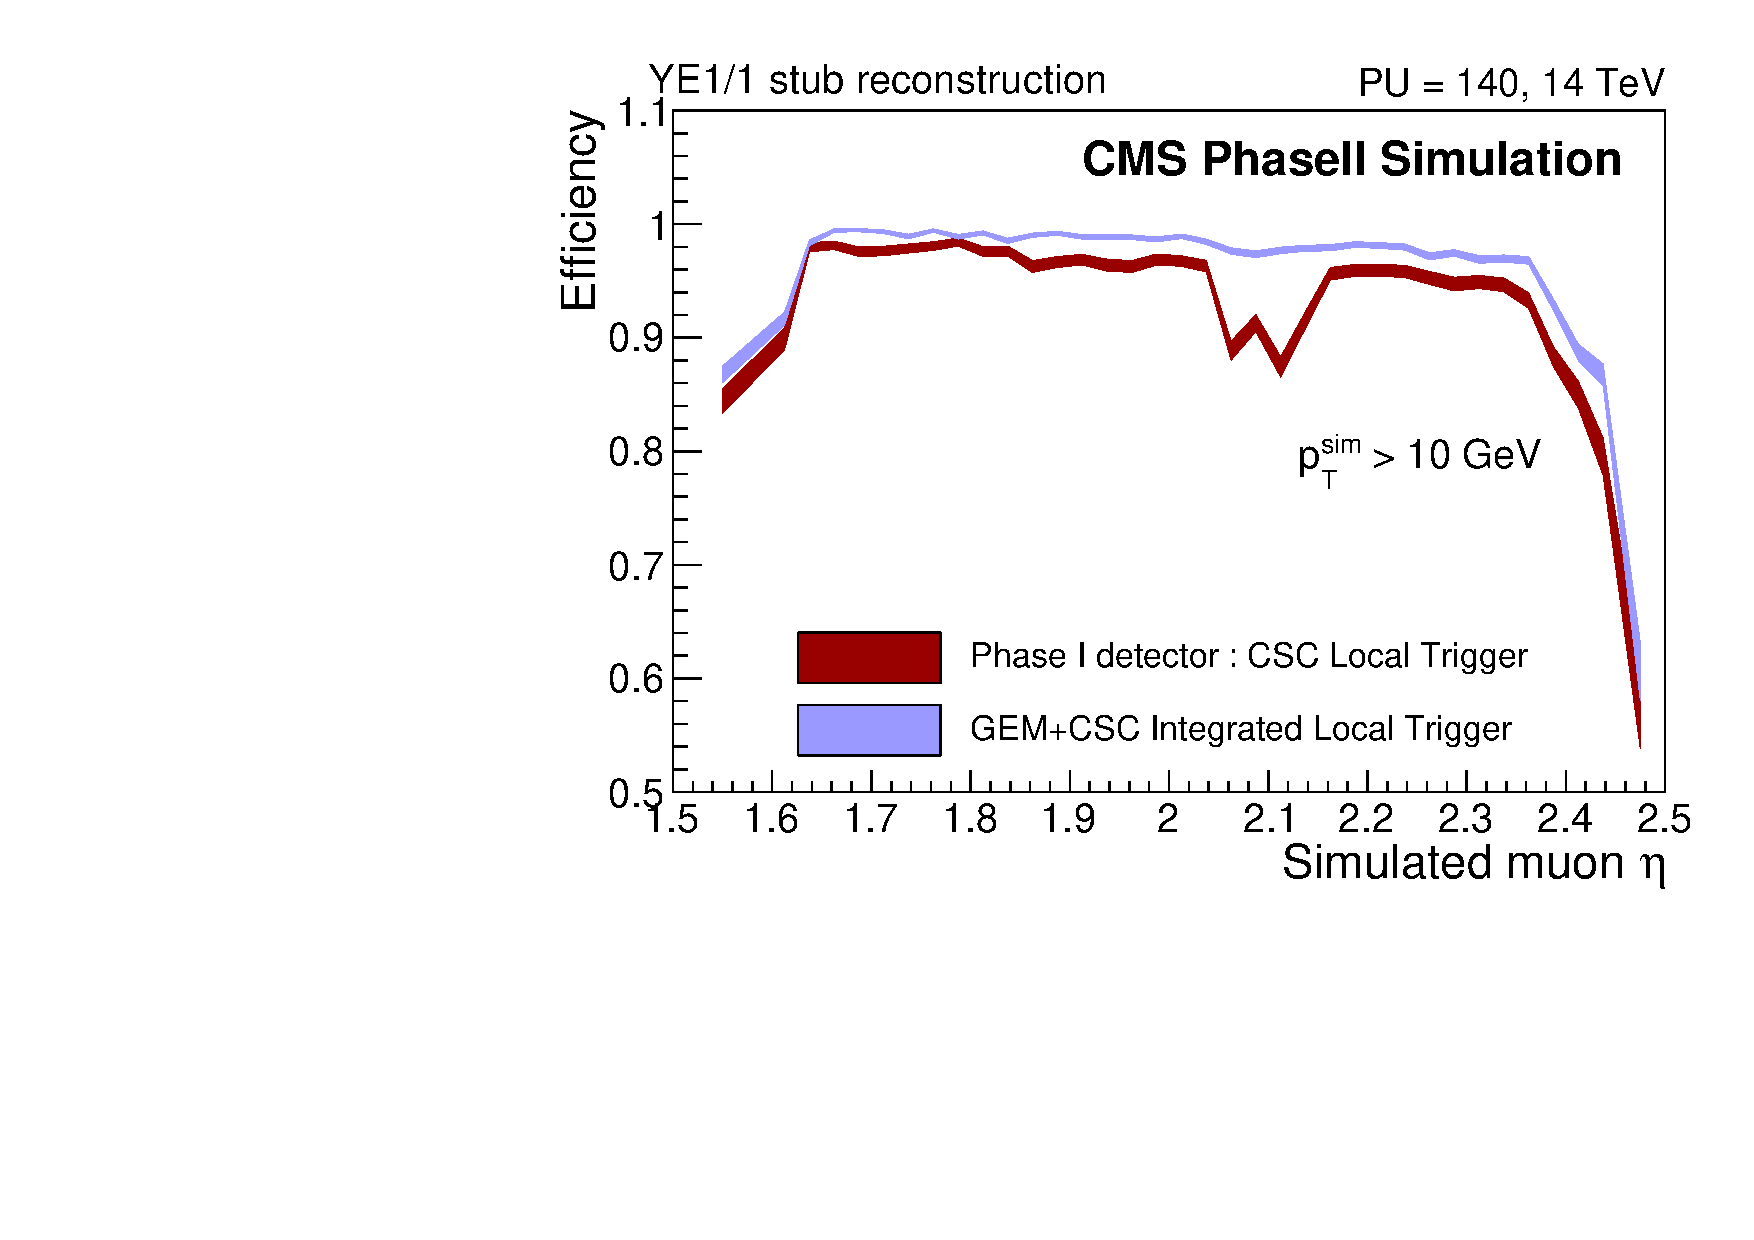
\includegraphics[width=\textwidth]{img/II-1-gem/gem-csc-efficiency.pdf}
      \caption{Left: reconstruction efficiency of the integrated GEM-CSC trigger as a function of the simulated muon |$\eta$|, compared to the same for the Phase-I CSC-only algorithm. Right: level 1 muon trigger rates before and after the GE1/1 upgrade at a luminosity of 2 $\times$ 10$^{34}$ cm$^{-2}$ s$^{-1}$. MS1/1 denotes the first endcap muon station level 1 trigger in both cases, i.e. with CSC-only or with the combination CSC and GEM trigger information \cite{Colaleo:2021453}.}
      \label{fig:II-1-gem-trigger}
    \end{figure}

    Preserving a low p$_T$ threshold is essential for the physics analysis to preserve good reconstruction efficiency of soft muons. These particles are important for a wide range of processes from beyond the standard model searches to measurments in the Higgs sector. Simulation studies have shown that in the case of $ H \rightarrow \tau^+ \tau^- $ where one $ \tau $ decays into a muon, a decrease of 5 GeV c$^{-1}$ in the p$_T$ threshold results in an increase of 35\% in the acceptance of the channel. In addition, the impact is not limited to the single muon trigger but affects all other triggers involving muons analysing for example $\mu+jet$ or $e/\gamma+\mu$ signals. \\

    To further improve the trigger efficiency of CMS, it is planned to add a new track trigger, a trigger system for the tracker, which would benefit from the high resolution of the subdetector. Forseen to be integrated during LS2, the system yields excellent results in the identification, reconstruction, and triggering of muons. However, due to the high occupancy of hits and the limited amount of computanional time alocated to the trigger, given approximations need to be done, degrading the results for certain physics channels. One of the assumptions made by the algorithms is that every particle originates from the interaction point. This has a significant impact on new physics processes involving hidden sectors of low interacting particles such as the decay of a Higgs into two neutralinos $ n $, which in turn create a so-called dark photon $ \gamma_d $
    \begin{equation}
      h \rightarrow 2 n_1 \rightarrow 2 n_d \gamma_d .
    \end{equation}
    The dark photon in turn decays into two muons which originate from a displaced vertex. Figure \ref{fig:II-1-gem-dark-photon} illustrates the limitations of the track trigger (red) to reconstruct muons in function of the distance between the vertex and the interaction point. Efficiency quickly drops to reach 0\% around 50 cm. The muon standalone trigger (blue) on the other hand is capable of reconstructing the track with high efficiency underlining the necessity of a preserving excellent trigger performances in the muon spectrometer.

    \begin{figure}[h!]
      \centering
      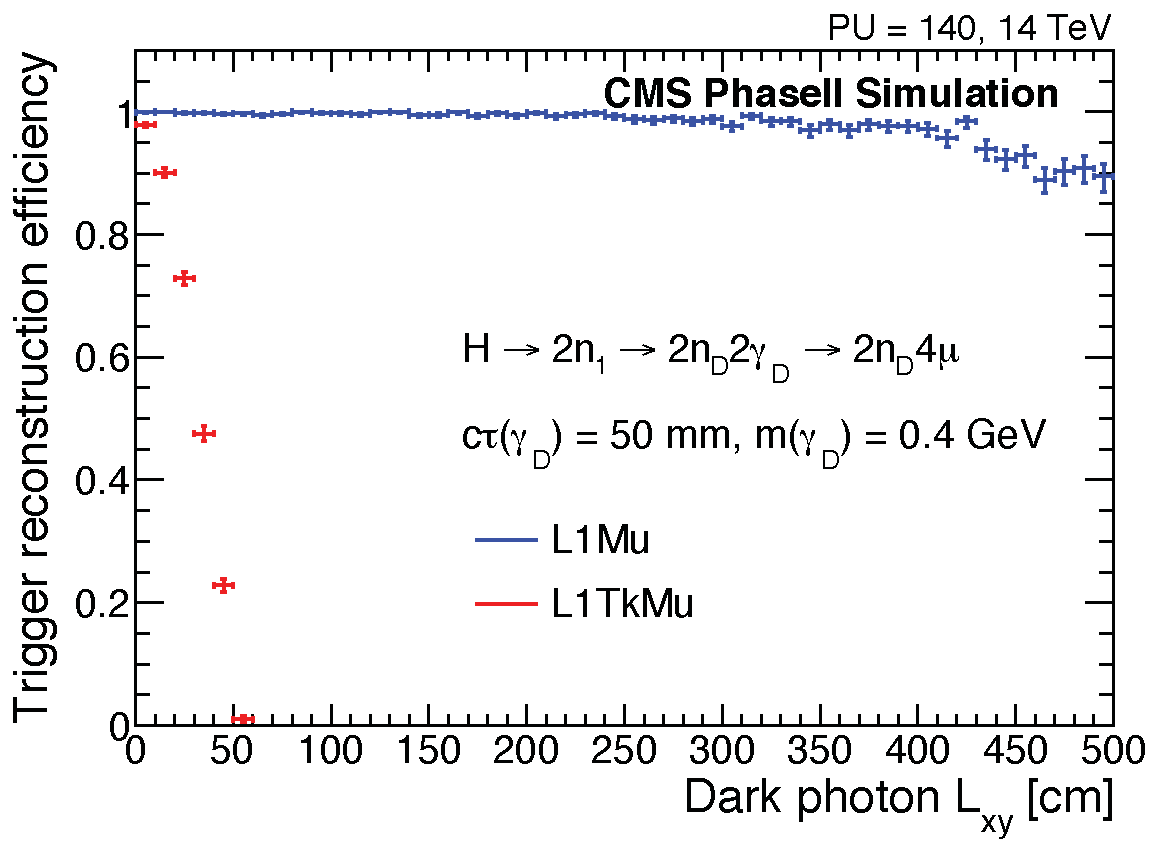
\includegraphics[width=0.6\textwidth]{img/II-1-gem/dark-photon.pdf}
      \caption{The probability of reconstructing at least one muon candidate produced in the decay of a light long-lived light particle decaying to a pair of muons $\gamma_d \rightarrow \mu \mu $ as a function of L$_{xy}$, the distance between the $\gamma_d$ decay vertex to the beamline in the transverse plane. Standalone muon trigger L1Mu performance is compared to that of L1TrkMu, a trigger based on matching muon and track trigger candidates with the CMS Phase-II detector simulation \cite{Colaleo:2021453}.}
      \label{fig:II-1-gem-dark-photon}
    \end{figure}

  \section{Technology Overview of Triple-GEM detectors}

    A GEM foil is a 50-$\mu$m-thick polymer foil covered with 5-$\mu$m-thin copper sheets on both sides chemically perforated by a high density of microscopic holes. The polymer used is either Kapton or Apical, both with a dielectric constant of 3.5. The holes are truncated double cones with an outer diameter of 70 $\mu$m and a inner diameter of 50 $\mu$m and are spaced by 140 $\mu$m on an hexagonal grid. The structure of the GEM foil as shown on the left in Figure \ref{fig:II-1-gem-holes}, is obtained using photolitography techniques that require precise aligment of the top and bottom masks. \\

    The diagram on the right in Figure \ref{fig:II-1-gem-holes} represents the electric field lines that appear when a high voltage difference is applied between the two layers of copper, typically on the order of 300 V, resulting in field densities inside the holes reaching approximatly 80 kV cm$^{-1}$. The structure of the electric field is used to amplify the signal of particles passing through the detector. Electrons resulting from the ionisation of the gas by charged particles are directed towards the holes of the foil. When reaching high kinetic energy inside the holes, they themselves ionize the medium, producing secondary avalanches of electrons. Each hole acts as a proportional counter with gains  \\

    \begin{figure}[h!]
      \centering
      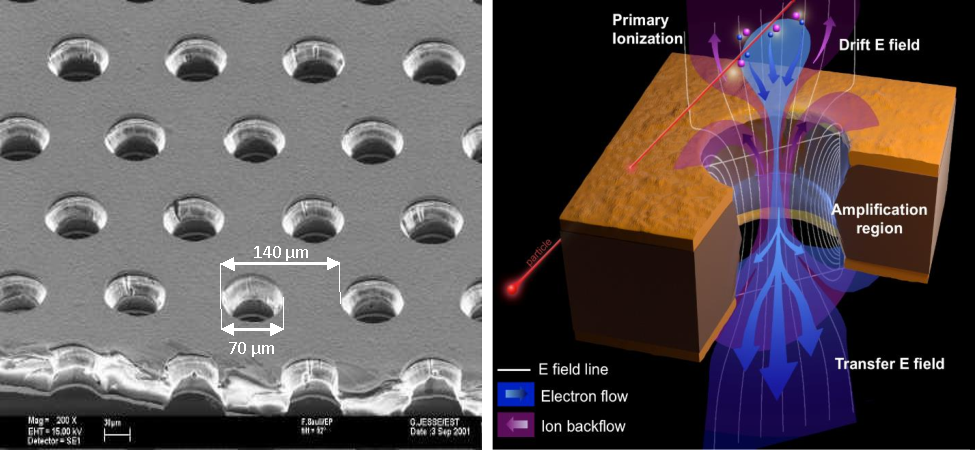
\includegraphics[width=\textwidth]{img/II-1-gem/holes.pdf}
      \caption{Left: scanning electron microscope picture of a GEM foil. Right: schematic view of the electric field lines (white), electron flow (blue), and ion flow (purple) through a bi-conical GEM hole \cite{Colaleo:2021453}.}
      \label{fig:II-1-gem-holes}
    \end{figure}

    To achive high gains in the detectors, two solutions can be implemented: increase the high voltage on the foils, or use multiple foils. The first option gives rise to discharges when operating at too high electric fields thus damaging the detector. Therefore, the choice to use three GEM foils has been made, hence the name of Triple-GEM detectors. The foils are arrangend as shown in Figure \ref{fig:II-1-gem-triple}. A drift cathode is placed on the top of the chamber which creates an electric field between itself and the top copper layer of the first GEM foil in the so-called drift gap measuring 3 mm. Electrons originating from the ionisation of the Ar/CO$_2$ gas mixture (70\% Argon, 30\% CO$_2$) by a charged particle drift towards the holes of the foil, while ions are collected by the cathode. Following, the electron shower is amplified by GEM 1, GEM 2, and GEM 3, respectivly tranfering the signal to the transfer 1, transfer 2, and induction gaps measuring 1 mm, 2 mm, and 1 mm each. The size of each gap is of importance in the detector performance and has been optimized over time to increase the speed of the signal and the detector efficiency. The current configuration is called 3/1/2/1 mm in reference to the gap size. In the induction gap, the drift of the electrons towards the anodes induces a signal on the latter which can be detected by electronics. \\

    \begin{figure}[h!]
      \centering
      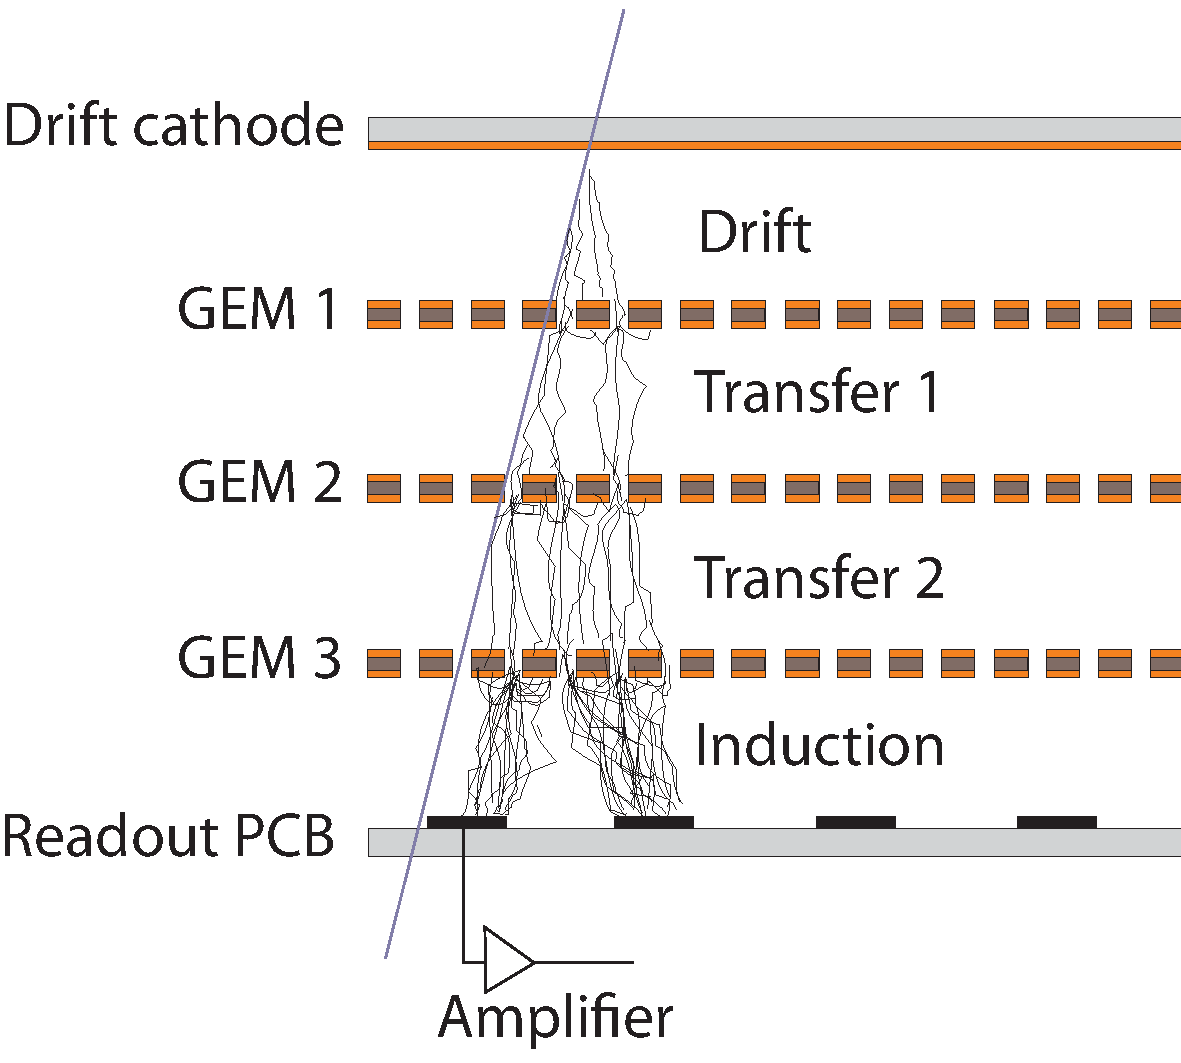
\includegraphics[width=0.5\textwidth]{img/II-1-gem/triple-gem-foils.pdf}
      \caption{Principle of operation of a generic triple-GEM chamber and definition of drift, transfer, and signal induction gap regions within the detector \cite{Colaleo:2021453}.}
      \label{fig:II-1-gem-triple}
    \end{figure}

  \section{Technical Design of GE1/1 chambers for CMS}

    The GE1/1 chambers are arranged in pairs to form superchambers, each covering 10$^o$ in $ \phi $ for a total of 72 chambers per endcap. The geometry of the superchambers is represented in Figure \ref{fig:II-1-gem-superchamber}. Due to mechanical constraint, the trapezoidal chambers are declined in two versions: a short one and a long one. The short chambers cover 1.61 < |$\eta$| < 2.18 and have a large base of 445 mm, a small base of 220 mm, and a height of 990 mm. The long chamers cover 1.55 < |$\eta$| < 2.18 and have a large base of 510 mm, a small base of 279 mm, and a height of 1283 mm. \\

    \begin{figure}[h!]
      \centering
      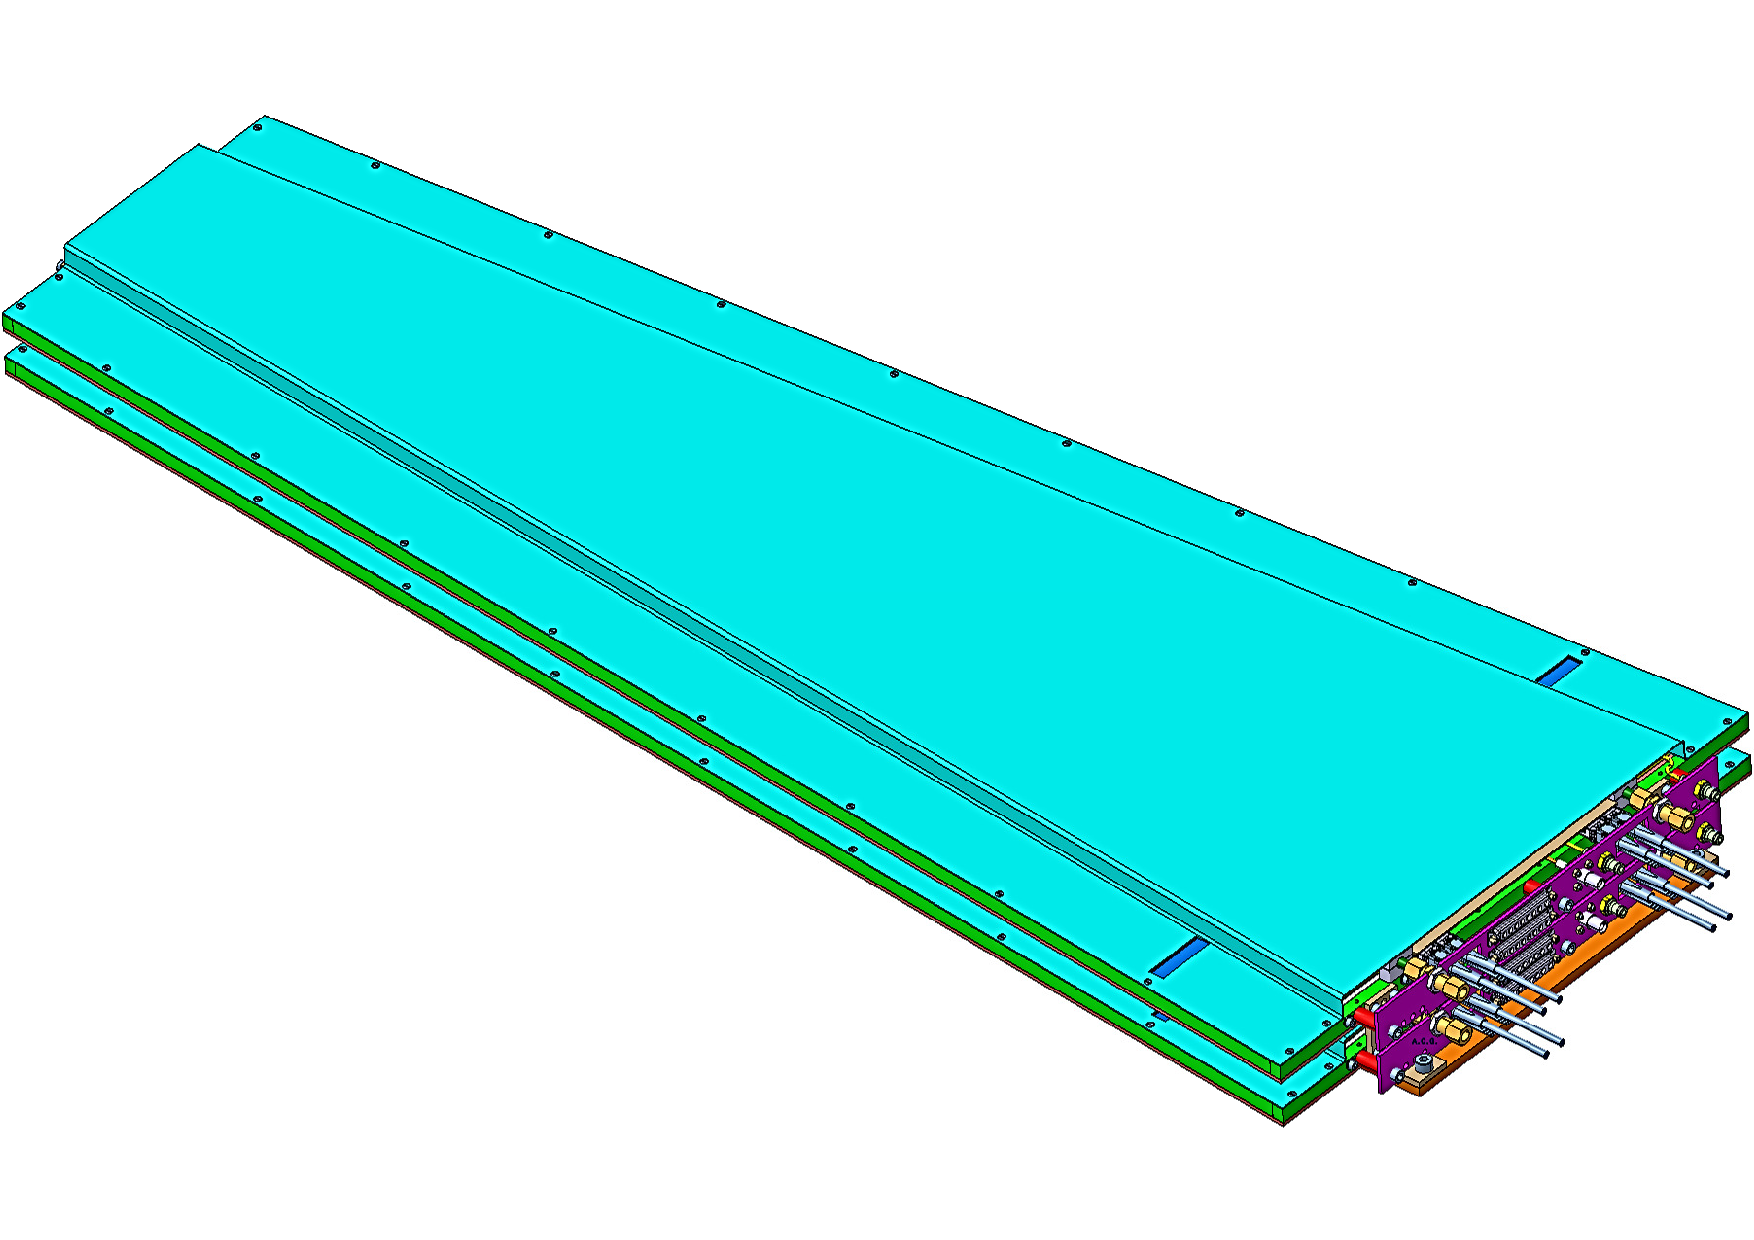
\includegraphics[width=0.6\textwidth]{img/II-1-gem/superchamber.pdf}
      \caption{A pair of GEM chambers form a superchamber \cite{Colaleo:2021453}.}
      \label{fig:II-1-gem-superchamber}
    \end{figure}

    The structure of a single chamber is shown in Figure \ref{fig:II-1-gem-exploded}. The drift cathode is placed on the bottom of the detector on which a frame is attached. The three GEM foils are streched out using screws embedded in the frame along with the seals making the chamber air tight. The anode strips are engraved on the readout board that closes the active region of the detector. One chamber is divided into three $ \phi $ sectors and eight $ \eta $ sectors with 128 strips running radially in each. This results in a mean coverage per strip of 450 $\mu$rad and a pitch varying from approximatly 500 $\mu$m to 1.3 mm. To each group of 128-strips a front-end electronics chip called the VFAT2 is attached. It digitizes the signals from the strips returning a single hit/not-hit bit. The VFAT2s are all connected to the GEM Electronics Board (GEB) which acts as router to forward the data towards the OptoHybrid (OH), a concentrator board located on the large side of the GEM which is the interface to the off-detector electronics. The VFAT2s and the OH are cooled down using cooling pipes attached on the top of the boards. Finally, a protective cover closes and protects the detector. When two chambers are assembled, a patch pannel is added in order to facilitate the insertion and removal of the low and high voltage cables, the water for the cooling, the gas, and the optical fibres connected to the DAQ system. Note that a signel source of high voltage is needed to power a chamber thanks to the use of a ceramic voltage divider which spreads the voltage over the various layers. \\

    \begin{figure}[h!]
      \centering
      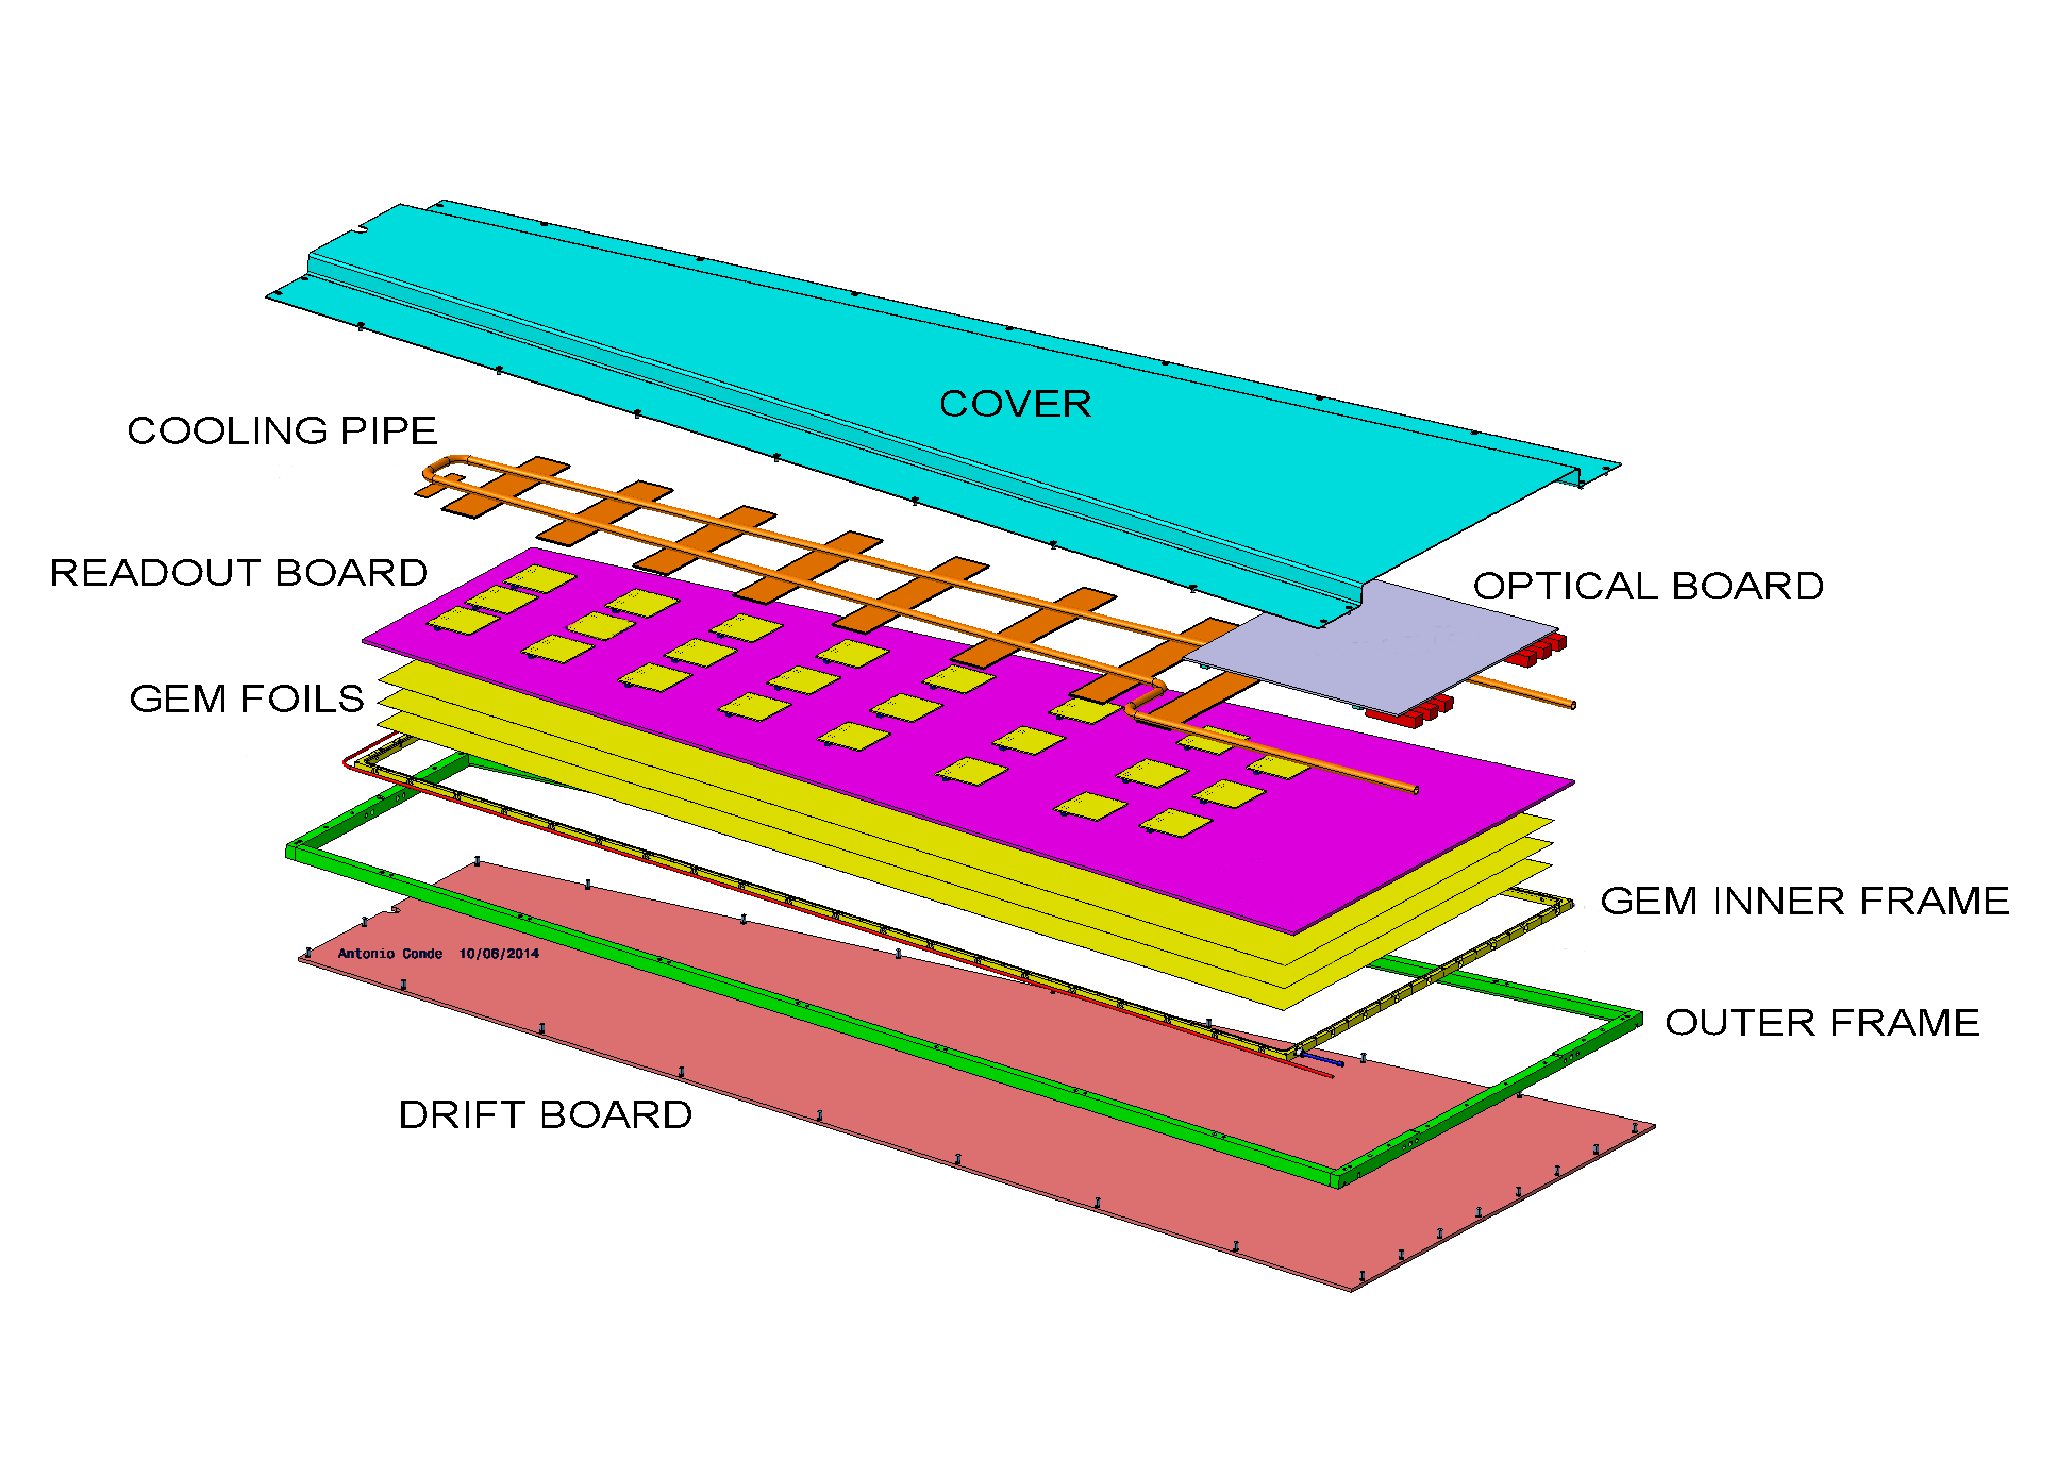
\includegraphics[width=\textwidth]{img/II-1-gem/gem-exploded.pdf}
      \caption{Exploded view of the mechanical design of a Triple-GEM chamber \cite{Colaleo:2021453}.}
      \label{fig:II-1-gem-exploded}
    \end{figure}

    Once assembled, the 72 superchambers will be installed in the endcaps of CMS as displayed in Figure \ref{fig:II-1-gem-wheel}. The full ring will be placed in the so-called nose of the endcap, between the HCAL and the ME1/1 stations.

    \begin{figure}[p]
      \centering
      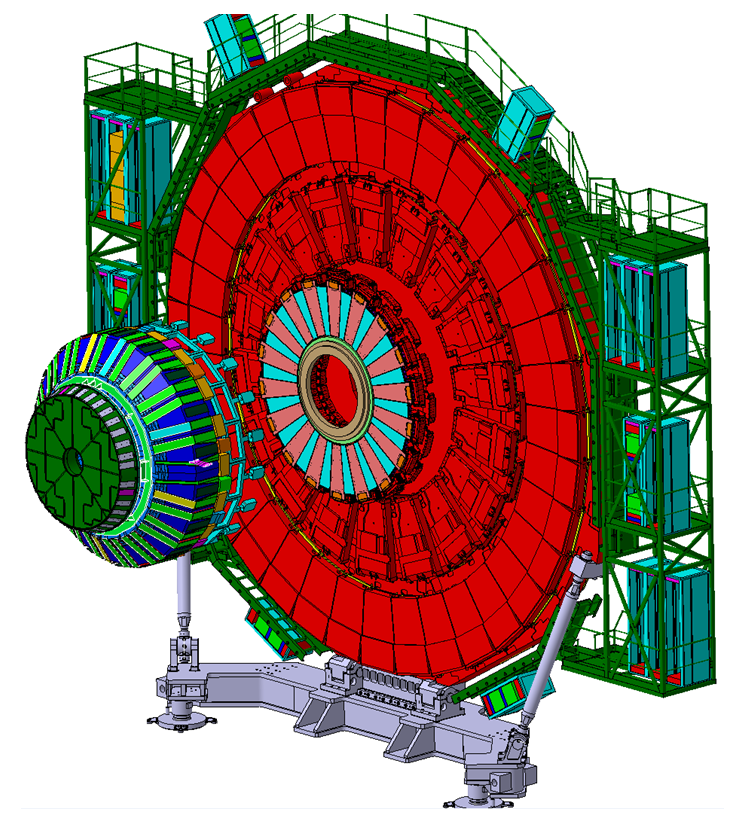
\includegraphics[width=\textwidth]{img/II-1-gem/wheel.png}
      \caption{First CMS muon endcap station where the inner ring is equipped with 18 long and 18 short triple GEM superchambers \cite{Colaleo:2021453}.}
      \label{fig:II-1-gem-wheel}
    \end{figure}

  \section{Detector Design Evolution}

    The design and fabrication method of the GE1/1 chambers has evolved over the past 5 years of R\&D. The five generations of detectors are shown in Figure \ref{fig:II-1-gem-generations}. GE1/1-I was the first 1-m-long prototype. It was equipped with only eight readout sectors, components were glued together and GEM foils were separated using spacers. The number of sectors was increased to 24 in GE1/1-II with the full granularity of the current design (384 strips per 10$^o$). The gap configuration was changed from 3/2/2/2 mm to 3/1/2/1 mm to increase the signal speed. From GE1/1-III and onwards, GEM foils were streched mechanically using an outer frame glued on the drift board. This design also introduced the use of a miniature ceramic high voltage divider to apply voltage on the foils. However, the assembly of the chamber induced mechanical tension on the readout board, deforming the detector and resulting in a non-uniform response. This problem was resolved in GE1/1-IV by pre-bending the boards in the opposite direction to compensate before being bolted to the frames. This geneation was the first assembled without glue, reducing production time to a few hours. However, the pre-beding technic did not yield viable results. Therefore, GE1/1-V uses pull-out pieces to tension the foils to the outer frame, on which the drift and readout board are bolted. The outer frame serves as a wall for the chamber and seales it using O-rings. Finally, the version of the design of the chambers that will be installed in CMS is GE1/1-VI which has optimized dimension to maximize the geometrical acceptance.

    \begin{figure}[h!]
      \centering
      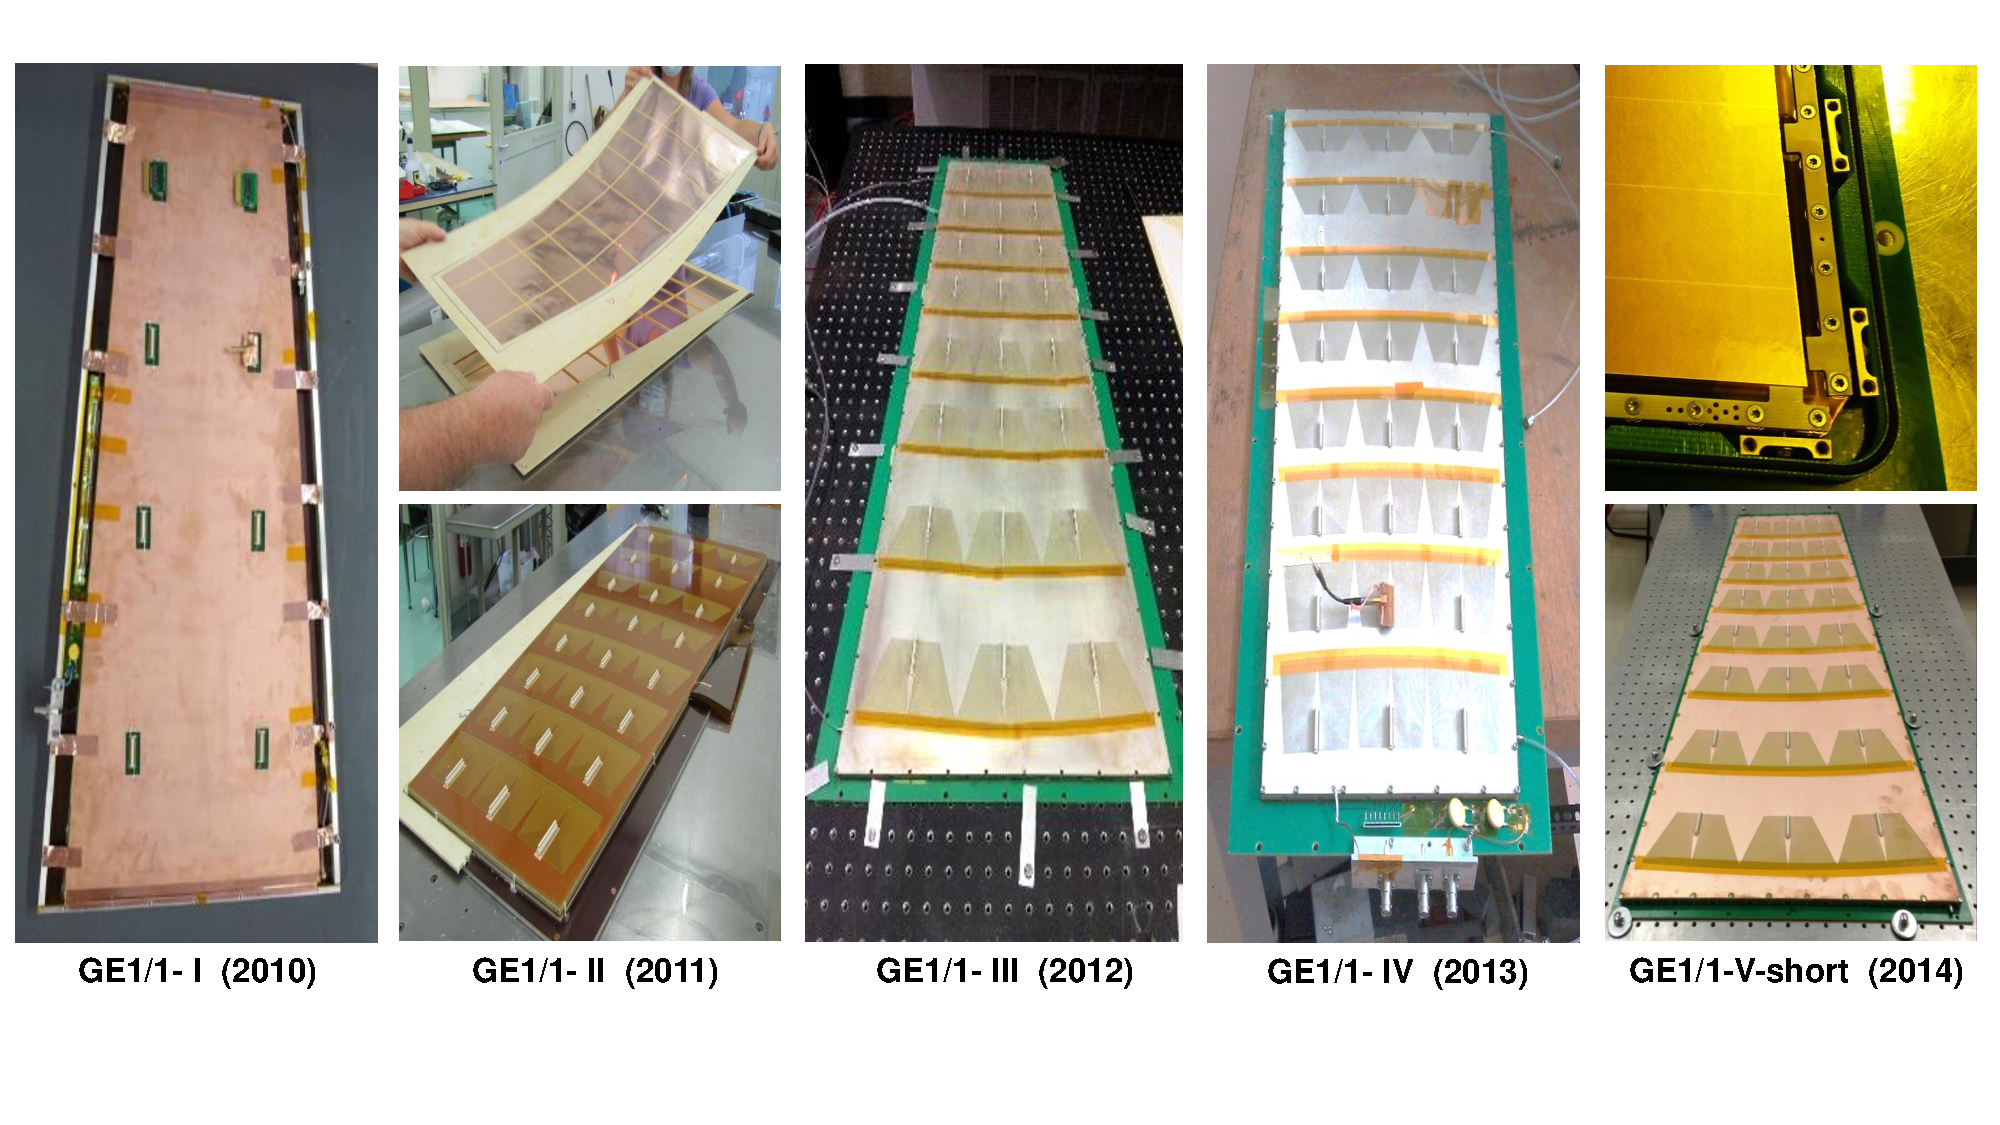
\includegraphics[width=\textwidth]{img/II-1-gem/generations.pdf}
      \caption{Five generations of GE1/1 prototype chambers constructed and tested by the GEM collaboration in 2010-2014. The split figures for GE1/1-II and GE1/1-V demonstrate the evolution from construction using spacer frames to purely mechanical stretching of GEM foils without any spacers \cite{Colaleo:2021453}.}
      \label{fig:II-1-gem-generations}
    \end{figure}

  \section{GE1/1 Prototyping Results}

    In order to provide the desired trigger and physics performance, the GE1/1 chambers must meet the following list of requirements:
    \begin{itemize}
      \item Maximum geometric acceptance within the given CMS envelope;
      \item Rate capability of 10 kHz cm$^{-2}$ or better to cope with the HL-LHC hit rate;
      \item Single-chamber efficiency of 97\% or better for detecting minimum ionizing particles resulting in 99.9\% efficiency for a superchamber when signals are combined with a logical OR;
      \item Angular resolution of 300 $\mu$rad or better on $ \Delta \phi = \phi_{GE1/1} - \phi_{ME1/1} $ to discriminate high-p$_T$ from low-p$_T$ muons;
      \item Timing resolution of 10 ns or better for a single chamber, which can be improved when combining the superchamber measurments, to allow matching with the CSC hits;
      \item Gain uniformity of 15\% or better across a chamber and between chambers to ensure that no geometrical or trigger biases are present. \\
    \end{itemize}

    Rate capability has been measured by monitoring the gain of a chamber when subject to a 22 keV Ag X-ray source and a high-intensity 8 keV Cu source. With Ar/CO$_2$, gain uniformity is maintained up to 100 MHz cm$^{-2}$, at which point the gain begins to drop. This confirms that the GE1/1 chambers are able to sustain rates up to 10 000 times higher than what they will experience in the 1.6 < |$\eta$| < 2.2 region of CMS. \\

    The detection efficiency is measured using a multi-layer tracking system placed in front of the detector in a beam of particles. Tracks are reconstructed in the former and extrapolated to the latter to match with reconstructed hits. When using the analog readout electronics, an offline cut is applied on the charge of the strips to cancel noise. In the digital readout system, an online threshold is applied. Both results indicate an efficiency plateau at 97\%. \\

    Using the above mentionned tracking system, the angular resolution of the GE1/1 chambers has also been measured during test beams. The resolution is taken to be the difference between the projected track position and the measured position in the detector. A resolution of 137$\pm$1 $\mu$rad has been obtained setting an upper limit on the angular resolution which is close to the theoretical value computed for a binary readout of
    \begin{equation}
      \frac{\text{angular strip pitch}}{\sqrt{12}} = \frac{455\  \mu\text{rad}}{\sqrt{12}} = 131\ \mu\text{rad} .
    \end{equation}
    Similar results were obtained using analog readout systems. \\

    The timing measurments are done by fitting the spread of the distribution plotting the time difference between a trigger seen by scintillators and the detection of the particle by the GEM detector. Time resolution studies have been performed using Ar/CO$_2$/CF$_4$ as well as Ar/CO$_2$ gas mixtures. The former yields as resolution of 4 ns due to the fast electron transport speed in CF$_4$ while the latter provides 8 ns. However, CMS has banned the use of CF$_4$ due to its toxicity effectivly selecting Ar/CO$_2$ at a ration of 70\% and 30\% respectivly to be the mixture used in the detectors. \\

    The response uniformity of the GEMs is measured for each detector as part of the quality control process. An X-ray generator is used to scan the entire chamber and the peak amplitude of the pulse charge distribution is taken as measurment of the uniformity. The latter does not vary more than 15\% accros the detector.
































  \section{GEM Upgrade Schedule}
 % T OK
  %   \cleardoublepage
  %
  %   \chapter{The GEM and CSC Data Acquisition Systems}
\label{chap:II-2-daq}

  The installation of GEM detectors in CMS and the integration with the CSCs require the development of a new DAQ system for the GE1/1 project. The understanding of the structure of both the GEM and CSC readout chains as well as the common CMS central DAQ is of importance in the scope of this thesis. To this end, all three systems are presented in details in the sections that follow. \\

  \section{The GE1/1 Data Acquisition System}

    The architecture of the GE1/1 DAQ system is represented in Figure \ref{fig:II-2-daq-gem-system}. It is divided into two sectors: the on-detector electronics on the left in charge of the managment of the detector, and the off-detector electronics on the right responsable for the data handling and the connection to the central DAQ. The two sectors are separated by a few douzen meters and connected through optical fibres. \\

    \begin{figure}[h!]
      \centering
      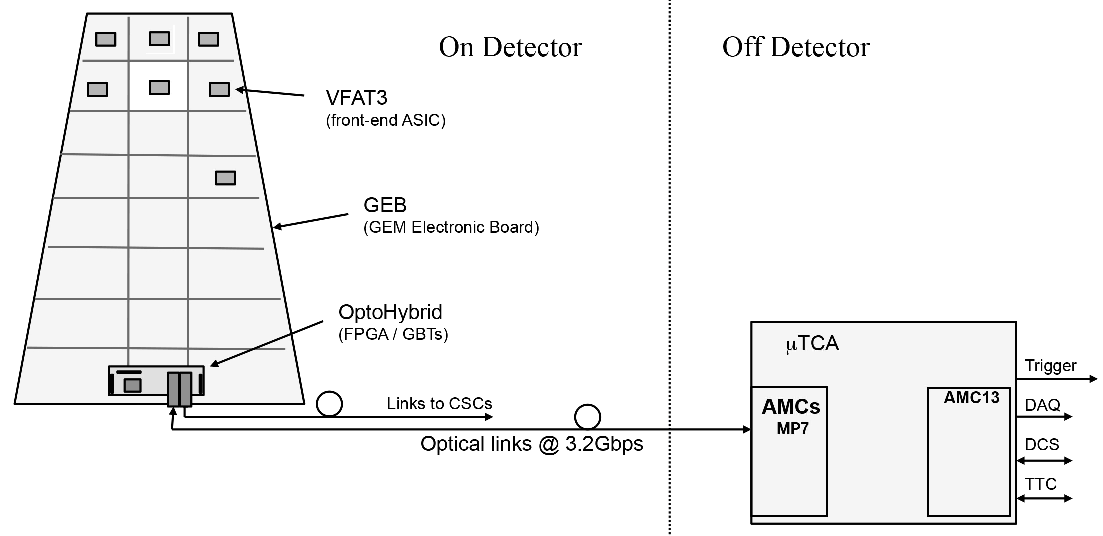
\includegraphics[width=0.7\textwidth]{img/II-2-daq/gem-system.pdf}
      \caption{??? \cite{Colaleo:2021453}.}
      \label{fig:II-2-daq-gem-system}
    \end{figure}

    The on-detector electronics focuses on the control and readout of the VFAT3 Application Specific Integrated Circuit (ASIC) which connects to the strips of the chamber and digitizes the data. The GEM Electronics Board (GEB), on which the VFAT3s are plugged in, then routes the signals to the OptoHybrid (OH) which acts as concentrator board and communication relay for the 24 VFAT3s. The communication with the off-detector system is performed through the GigaBit Tranciever (GBT) chipset and the Versatil Link installed on the OH. Both projects are led by CERN and provide radiation hard tools for LHC experiments. \\

    On the off-detector side, the Micro Telecommunications Computing Architecture (microTCA, MTCA, or $\mu$TCA) \cite{PICMG} crate standard is used to power and monitor the Advanced Mezzanine Cards (AMCs) which provide the ressources to communicate with the on-detector electronics. Links from multiple OHs are concentrated on one MP7 AMC which formats the data and transfers it to the CMS AMC13 mezzanine. The AMC13 is the link between the microTCA crate and the central DAQ of CMS which provides the clocking, trigger, and control over the system. The control of the DAQ chain is performed from a XDAQ application using the IPBus protocol over ethernet.

    \subsection{The VFAT3 ASIC}

      The VFAT3 ASIC is a binary front-end chip optimized for gaseous detectors which function is to digitize the analog signals coming from the detector and provide fast trigger and tracking data. The trigger data is sent at the LHC clock over a fixed latency path and then used in the algorithms of the L1 trigger to accept or reject events. The tracking data holds the full granularity information of the events that have been accepted and follows a variable latency path. The logic diagram of the chip is shown in Figure \ref{fig:II-2-daq-vfat3}. It is made of an analog front-end which amplifies, shapes, and digitizes the signal from the GEM strips, and of a digital back-end for slow control, fast control, and data readout. \\

      \begin{figure}[h!]
        \centering
        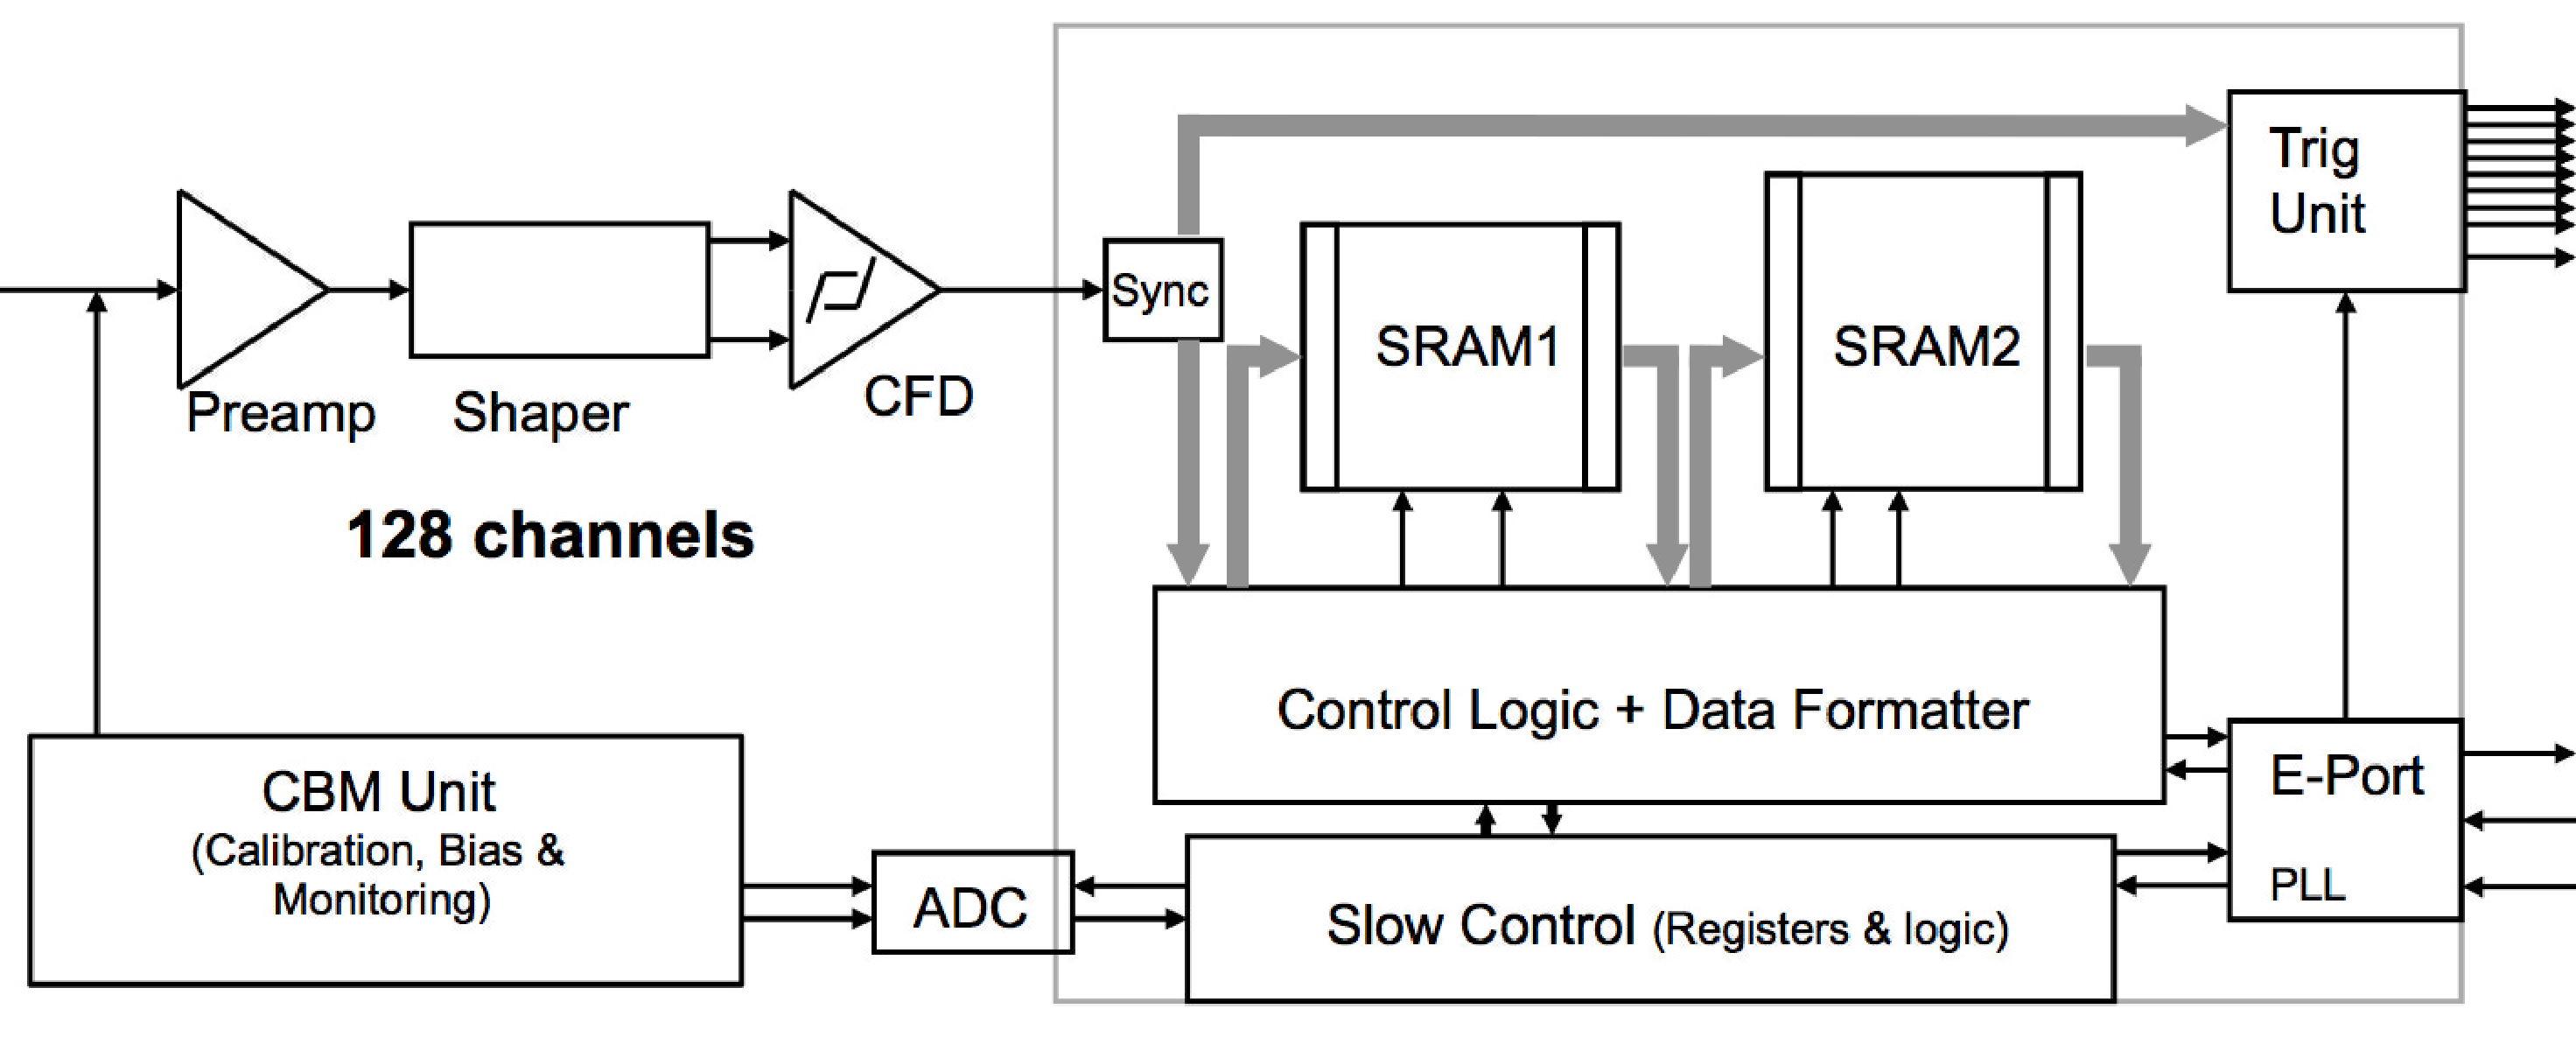
\includegraphics[width=\textwidth]{img/II-2-daq/vfat3.pdf}
        \caption{??? \cite{Colaleo:2021453}.}
        \label{fig:II-2-daq-vfat3}
      \end{figure}

      \paragraph{The analog front-end} is further optimized for the readout of GEMs in particular. It is composed of 128 channels which amplify and shape the analog signals from the strips with programmable shaping times to allow for various integration lengths of the signal. According to the gas mixture, signal charge from the GEM can last for approximatly 60 ns. Increasing the shaping time to fully integrate the charge will result in a higher signal to noise ratio. Simulations performed on the analog front-end show that a time resolution of 7 ns can be achieved by using a Constant Fraction Discriminator (CFD) with a shaping time of 50 ns. After shaping, the amplitude of the analog signal is compared against a programmable threshold by a comparator to yield a binary output flag for each channel. \\

      \paragraph{The fixed latency path} is used to provide a fast hit information to the trigger system of CMS at a frequency equal to the LHC clock of 40 MHz. The trigger unit inside the VFAT3 formats the output of the 128 comparators and transmits it over 8 differential pairs at a rate of 64 bits per BX. It allows to either encode a logical-OR of two adjacent strips effectivly dividing the number of bits to send by a factor two, or use a zero supression algorithm to solely transmit information on hit strips. Ensuring a fixed latency on this path in crucial to maintain predictability in the trigger system and identify the correct BX. \\

      \paragraph{The variable latency path} is activated upon reception of an L1A to transmit the full granularity information on an event that has been accepted by the trigger system. The VFAT3 holds two Static Random-Access Memories (SRAMs) which are used to store events. The SRAM1 is a circular buffer filled at a frequency equal to the LHC clock with the output of the 128 comparators. When the VFAT3 receives an L1A, it transfers a given event from the SRAM1 to the SRAM2 and adds the BX Counter (BC) and the Event Counter (EC), which respectivly count the number of BX elapsed and the number of L1A received, to the event data. To determine which event needs to be transfered, the chip uses a programmable parameter called the latency that informs the system on the delay between the digitization of an event and the arrival of an L1A corresponding to the same event. It is a measures of the response time of the trigger system to a given event which is a fixed delay. Events stored in the SRAM2 are then formated and sent over a single differential pair out of the VFAT3. The formatting of the data can be selected using a programmable register to be either lossless or zero suppressed. \\

      \paragraph{The slow control} module handles the configuration of the internal registers of the VFAT3. These registers define quantities such as the threshold of the analog front-end, the latency, the readout data format, etc. Coupled with the Calibration, Bias \& Monitoring (CBM) unit, it allows to perform calibration routines on the chip. \\

      \paragraph{The fast control} defines all the time sensitive commands that the VFAT3 receives. These are the Event Counter 0 (EC0), Bunch Counter 0 (BC0), Calibration Pulse (CalPulse), Resynchronisation (Resync), and L1A. The EC0 and BC0 commands respectivly reset the EC and BC; the CalPulse is used to send a calibration pulse on given strips in order to callibrate the analog front-end; the ReSync command resets the internal pointers; and the L1A informs the VFAT3 that an event needs to be transfered to the DAQ.

    \subsection{The GEM Electronics Board}

      The limited space in which the GEM detectors will be installed constrains the design of the system by making it impossible to run flat cables for the 24 VFAT3s. Therefore, the GEB, a Printed Circuit Board (PCB) of the same dimension as the GEM detector, was designed to route the signals of the front-end chips to the OH located on the large side of the detector, furthest away from the beam pipe. A picture of a prototype of the GEB is shown on the right in Figure \ref{fig:II-2-daq-geb}. The functions of the GEBs are to host the VFAT3 ASICs connected to the 24 sectors of the GEM readout board, route their signals to the OH, distribute power to the chips, and provide electric shielding to the detector. The GEB is divided into three columns of eight VFAT3s, further divided into two sectors each as represented in the left picture in Figure \ref{fig:II-2-daq-geb}. The clock, slow control, and fast control are commonn for each column. \\

      \begin{figure}[h!]
        \centering
        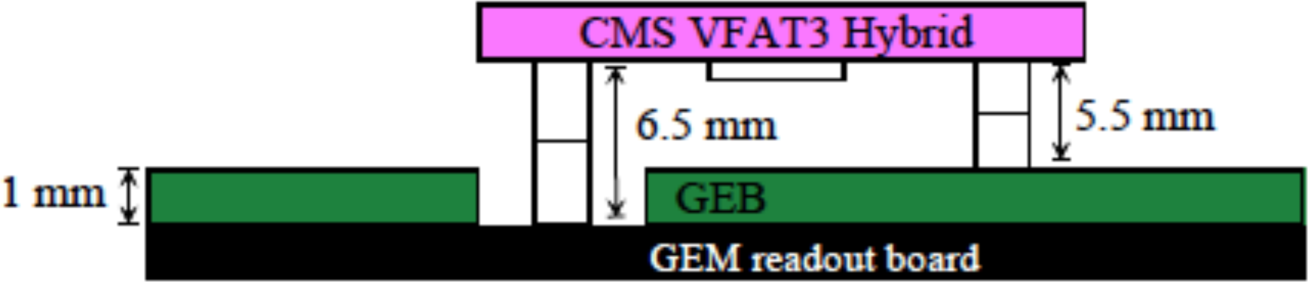
\includegraphics[width=0.8\textwidth]{img/II-2-daq/geb.pdf}
        \caption{??? \cite{Colaleo:2021453}.}
        \label{fig:II-2-daq-geb}
      \end{figure}

      The VFAT3s are soldered on the GEB and connected to the GEM readout board on which it rests through a flexible PCB. The control and data signals from the chips are routed on the PCB towards four connectors located on the large side of the detector which connect to the OH. The power for the VFAT3s and the OH is distributed by the GEB using radition hard DC/DC converters developped by CERN which convert the incoming low voltage to the required voltages. In addition, the bottom layer of the GEB is grouded proving shielding to the detector from external ElectroMagnetic Interference (EMI).

    \subsection{The OptoHybrid}

      The OH is the interface between the VFAT3 ASICs and the off-detector system. It is a 10 cm $ \times $ 20 cm board mounted on the GEB equipped with a Field Programmable Gate Array (FPGA) and Integrated Circuits (ICs) dedicated to the operation of the optical links. The FPGA solely handles the trigger data by applying zero suppression algorithms, formatting the data, and sending it to the CSC and the GEM trigger system separatly over two optical links using the SFP+ connectors. The other functions of the VFAT3s are directly connected to the three GBT chipsets installed on the OH. Each GBT chipset is capable of handling a column of eight VFAT3s.

    \subsection{The GBT and Versatil Link}

      The GBT \cite{Moreira:1235836} and Versatil Link \cite{Soos:1609037} are projects developped by CERN providing radiation hard tools for optical communication to the LHC experiments. The GBT is an optical data link technology providing bidirectionnal 4.8 Gb/s (Gigabits per second) serial communication designed to connect the on-detector and off-detector electronics. It is declined in two version: the GBTX which is a radiation hard ASIC, and the GBT-FPGA which is a core that can be implemented inside an FPGA. Complementary to the GBT which provides the data structure and communication protocol between components, the Versatil Link project develops radiation hard optical transceivers. The integration of the GBTX, Verstil Link, and GBT-FPGA projects is shown in Figure \ref{fig:II-2-daq-gbt-versatile}. \\

      \begin{figure}[h!]
        \centering
        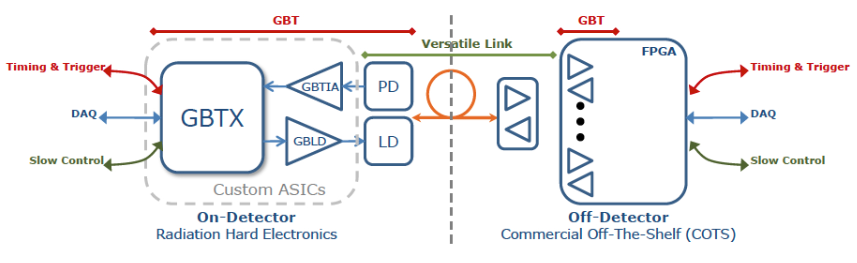
\includegraphics[width=\textwidth]{img/II-2-daq/gbt-versatile.pdf}
        \caption{??? \cite{Moreira:1235836}.}
        \label{fig:II-2-daq-gbt-versatile}
      \end{figure}

      The GBT defines a data format shown in Figure \ref{fig:II-2-daq-gbt-frame}. The stream of data is divided into frames of 120 bits transmitted at 40 MHz, resulting in a data rate of 4.8 Gb/s from which 3.36 Gb/s are accessible by the user. The frame start with a four bits header (H) which defines the frame type and ends with 32 bits of Forward Error Correction (FEC). The error correction is done by encodeding the data using a Reed-Salomon code that can correct bit flips due to radiation. The 84 remaining bits are user accessible. The first two bits are used for internal slow control (IC) and the two following bits for external slow control (EC), leaving 80 bits of data (D) accessible to the user for DAQ, TTC, and slow control purposes. \\

      \begin{figure}[h!]
        \centering
        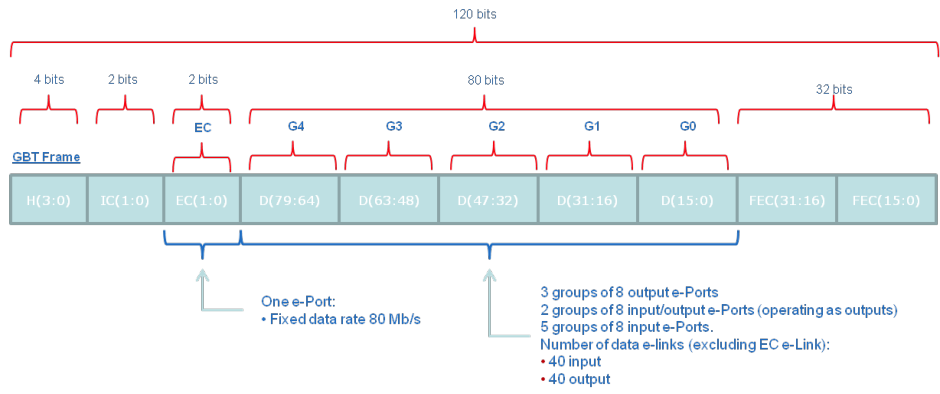
\includegraphics[width=\textwidth]{img/II-2-daq/gbt-frame.pdf}
        \caption{??? \cite{Moreira:1235836}.}
        \label{fig:II-2-daq-gbt-frame}
      \end{figure}

      The header is used to syncrhonize the link by requiering the detection of a series of valid header fields. It is therefore protected by the FEC in order to ensure efficient frame-locking. From the slow control bits, both running at 80 Mb/s, the IC is reserved for the control and monitoring of the GBTX while the EC on the other hand can be freely assigned by the user. The data field is used to transfer DAQ, TTC, and slow control requests to the various subsystems connected to the GBT and can implement any user defined protocol. The FEC uses two Reed-Salomon codes interleaved with 4-bit symbols each capable of correcting double errors. This means that the total frame can recover up to 16 corrupted bits. Additionnaly, the GBT frame is scrambled in order to maintain DC balance on the transmission lines. \\

      On the FPGA side, the communication protocol is seen by the user as a 84-bits-wide vector that is sampled at a frequency of 40 MHz an then formatted by the GBT-FPGA core. The GBTX ASIC on the other hand uses 42 Electric serial Links (E-Links) to handle the data. The structure of the GBTX is shown in Figure \ref{fig:II-2-daq-gbt-asic}. Each E-Link is composed of three differential pairs: one to transmit and one to receive the data, and one to carry the clock synchronuous to the data. From the 42 E-links, one is dedicated to the IC and one to the EC, each transfering data at 80 Mb/s by serializing the two IC or EC bits of the GBT frame on a single link. The use of the remaining 40 E-Links is defined according to the speed at which they operate. The 80-bit-long user data can be configured to either be serialised by a factor two, four, or eight resuling in the use of 40, 20, or 10 E-Links respectivly running at 80 MHz, 160 MHz, or 320 MHz to accomodate the data rate. For the GEM project, a serialisation factor of eight is used, meaning that from the 40 E-Links, only 10 are in used, each of them tranfering 8 bits per BX. \\

      \begin{figure}[h!]
        \centering
        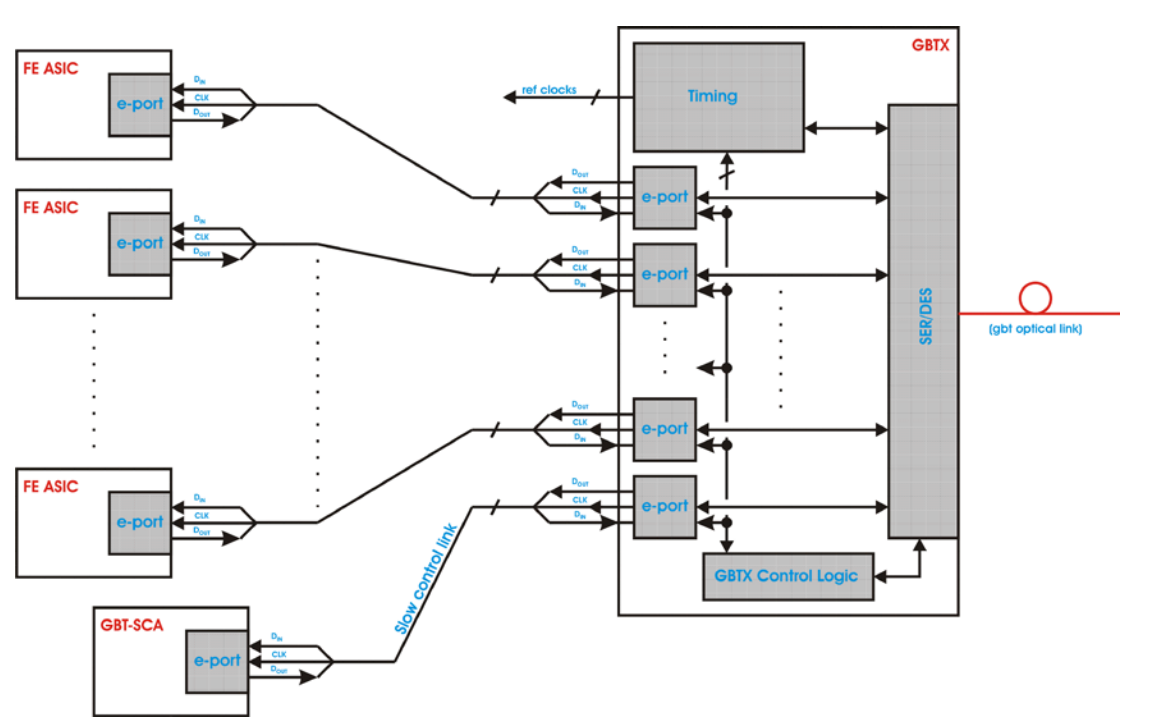
\includegraphics[width=0.8\textwidth]{img/II-2-daq/gbt-asic.png}
        \caption{??? \cite{Moreira:1235836}.}
        \label{fig:II-2-daq-gbt-asic}
      \end{figure}

      To convert the GBTX signals into optical communication, the Versatil Link project provides two laser diode modules: a transceiver module called VTRx and a dual transmitter module called VTTx. The modules have been designed to wistand high magnetic field and radiation doses as encountered in the LHC experiments. The maximal bit rate is of 4.8 Gb/s with a bit error rate inferior to 10$^{-12}$.

    \subsection{The microTCA Standard}

      The off-detector electronics is implemented using the microTCA crate standard to manage the back-end system. The microTCA standard was developped for the telecommunication industry as a successor for the Advanced Telecommunications Computing Architecture (ATCA) technology. It uses a smaller form factor for the AMCs declines into a single width (73.8 mm $ \times $ 181.5 mm) or double width (148.8 mm $ \times $ 181.5 mm) version. The key feature of the crate is the topology of the backplane connecting the AMCs. The latter is not defined in the specifications but often implements a dual-star network which provides reduduncy and thus avoid critical failures of the system upon malfunction of a component. \\

      The structure of the crate is shown in Figure \ref{fig:II-2-daq-utca-crate}. Managment and control of the subsystems of the crate are performed by the MicroTCA Carrier Hub (MCH), which in failure critical systems can be accompagnied by a second MCH for redunduncy. These two MCHs are the central points of the network in dual-star topology. They communicate with the Cooling Units (CUs), Power Modules (PMs), and AMCs through the Intelligent Platform Management Interface (IPMI). The CUs and PMs are equipped with a Enhanced Module Managment Controller (EMMC) and the AMCs with a Module Managnment Controller (MMC) which are used to communicate with the MicroTCA Carrier Management Controller (MCMC) of the MHCs. These controllers implement the IPMI protocol and provide system managment functions to the crate. Upon power-on of the crate or hot-swap of an AMC, the MCHs provide minimal power to the EMMCs and MMCs through dedicated lines in order to start the initial transaction sequence. During this exchange, the power requirements of the modules are defined and a boot-up sequence takes place. Once the transaction is closed, power is provided to the rest of the module and normal operation begins. A power-off sequence takes place when the crate is shutdown or an AMC is removed. \\

      \begin{figure}[h!]
        \centering
        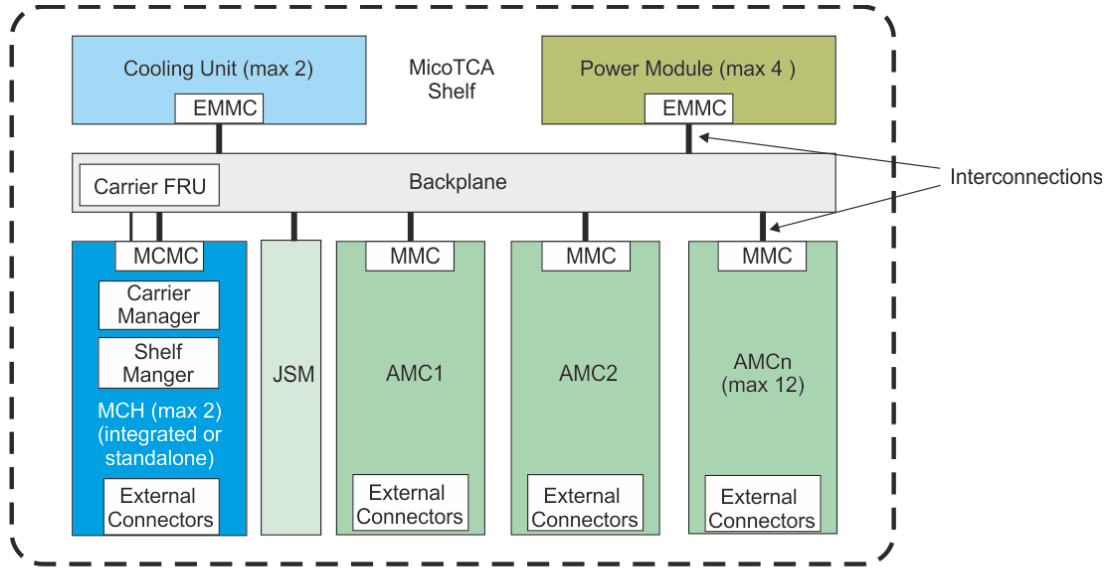
\includegraphics[width=\textwidth]{img/II-2-daq/utca-crate.png}
        \caption{??? \cite{VADATECH}.}
        \label{fig:II-2-daq-utca-crate}
      \end{figure}

      The backbone of the microTCA crate is its backplane. It provides point to point connections between the AMCs and MCH to AMC connections. The interconnects between elements are called fabrics and are what defines the topology of the crate. On the AMCs, the connections to the backplane are called ports. In the dual-star topology, each fabric is duplicated and connected to a separate MCH. As the backplane topology is not described in the specifications of the standard, a common topology is described.
      \begin{itemize}
        \item Fabric A is used for Gigabit Ethernet communication between the AMCs and MCH1 on port 0 and the MCH2 on port 1.
        \item Fabric B is allocated for technologies such as Seriel-ATA through port 2 and 3 for the MCH1 and MCH2 respectrivly.
        \item Fabric C is only used in single MCH mode and uses port 3 to connect the AMCs to MCH1.
        \item Fabric D to G are fat pipes which use multiple protocol agnostic links to connect the AMCs to the MCH1 on ports 4 to 7 and to the MCH2 on ports 8 to 11.
        \item Some backplanes implement point to point communication between ACMs on ports 12 to 20 following a custom interconnect.
      \end{itemize}
      Next to signal busses, the microTCA standard defines three clocks busses that can originate from the MCHs or the AMCs.

    \subsection{The MP7 Advanced Mezzanine Card}

      The AMC board used as back-end electronics is the MP7 \cite{MP7} developped by Imperial College and shown in Figure \ref{fig:II-2-daq-mp7}. It is equipped with a large Virtex-7 FPGA providing extensive computanionnal power. The optical interface with the on-detector electronics is done through six Avago MiniPOD transmitters and six Avago MiniPOD receivers for a total of 72 bidirectionnal links. Using one MP7, 9 superchambers can be readout thus requiering a total of 8 MP7s for the GE1/1 project. \\

      \begin{figure}[h!]
        \centering
        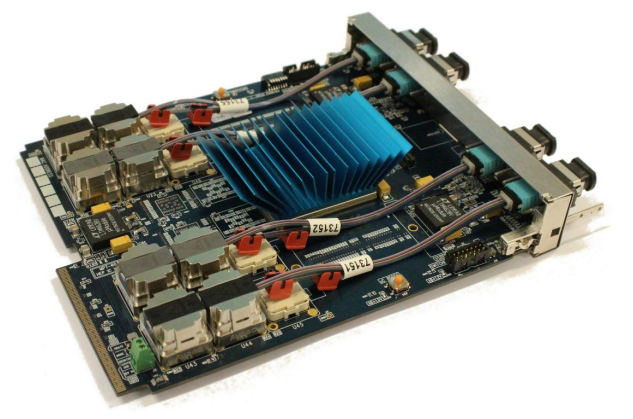
\includegraphics[width=0.8\textwidth]{img/II-2-daq/mp7.png}
        \caption{??? \cite{MP7}.}
        \label{fig:II-2-daq-mp7}
      \end{figure}

      The function of the MP7 is tripe: handle slow control requests for the subsystems, interpret TTC signals, and readout the trigger and tracking data from the OHs. The MP7 is the interface between the control and monitoring software and the detector electronics. It uses the fabric A lines of the MCH1 to connect to a Gigabit Ethernet network and handle TCP/IP requests. It interprets the requests and forwards them to the appropriate subsystem: either itself or over the optical link to the OHs and VFAT3s. The MP7 also receives the TTC commands on the fabric B from MCH2 and must forward them to the subsystems along with the LHC clock received on the CLK1 line. Finally, when the VFAT3s or the OHs push data upwards to the MP7, the latter must format the data before sending it on the backplane to a dedicated DAQ AMC.

    \subsection{The AMC13}

      The module which delivers the TTC signals and the LHC clock to the MP7s and retreaves the trigger and tracking data from the backplane is the AMC13 \cite{AMC13}. It is a board specifically designed for CMS which replaces the MCH2 is the microTCA crate. Its functionnal diagram is shown in Figure \ref{fig:II-2-daq-amc13}. It is equipped with two FPGAs: a powerfull Virtex-6 for data handling, and a smaller Spartan-6 for control and monitoring. The TTC signal is received through an optical link from which the LHC clock is extracted along with the TTC commands. The clock is forwared on the CLK1 line and the TTC commands are passed to the Spartan-6 FPGA which formats them on the fabric B lines at 80 MB/s. Being in the MCH2 slot, the AMC13 has direct access to all AMCs, which it uses to retreive tracking and trigger data over the fabric A ports running at 5 Gb/s. For development purposses, the AMC13 integrates internal TTC commands and LHC clock generators. \\

      \begin{figure}[h!]
        \centering
        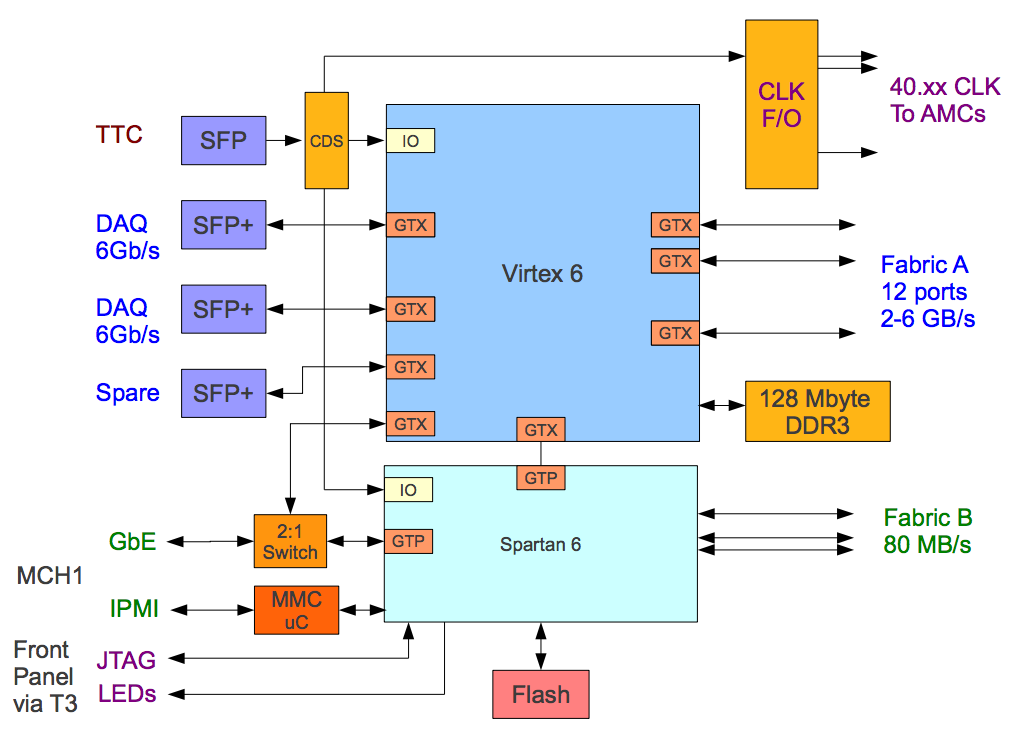
\includegraphics[width=\textwidth]{img/II-2-daq/amc13.png}
        \caption{??? \cite{AMC13}.}
        \label{fig:II-2-daq-amc13}
      \end{figure}

      The Virtex-6 FPGA of the AMC13 is connected to the central DAQ of CMS through the two SFP+ optical links running at 6 Gb/s which implement the S-Link Express protocol defined by CMS. An additionnal SFP+ can be used as spare if the bandwidth is required. Next to the data, the AMC13 also send TTS signals to the TCDS system to inform it about the status of the readout. The TTS codes can be: hardware failure, imminent overflow, sync lost, busy, ready, or error. Using these, the TCDS system can regulate the L1A rate for the system to be able to cope.

    \subsection{The IPBus Protocol}

      To communicate between the control and monitoring applications and the subsystems, a new protocol called IPBus has been developped for the CMS subdetectors. It uses the Internet Protocol (IP) and can be sent over User Data Protocal (UDP) or Transmission Control Protocol (TCP). IPBus transactions are simple read/write operations using a A32/D32 implementation (Address of 32 bits, Data of 32 bits). A sequence of transactions is called a packet which starts with a packet header of 32 bits which format is shown in Figure \ref{fig:II-2-daq-ipbus}. \\

      A transaction is always performed in two stages: a request from the applications is sent to which the system provides a response. The header of the request specifies the request type and request size. Additionnal 32 bits words are added in function of the type of operation to perform. For a read operation, the base address of the read must be specified. The response will contain N 32 bits words corresponding to the data at the base address and the incremental N addresses where N is the size of the request defined in the header. For a write operation, the request will contain the base address followed by N 32 bits words that should be written at the base address and the N following addresses where N is the size of the request defined in the header. The response will be a single header containing a status code. Variation of the read/write operations exist such as the FIFO-read and FIFO-write, which repeatevly read and write words at the same address. \\

      \begin{figure}[h!]
        \centering
        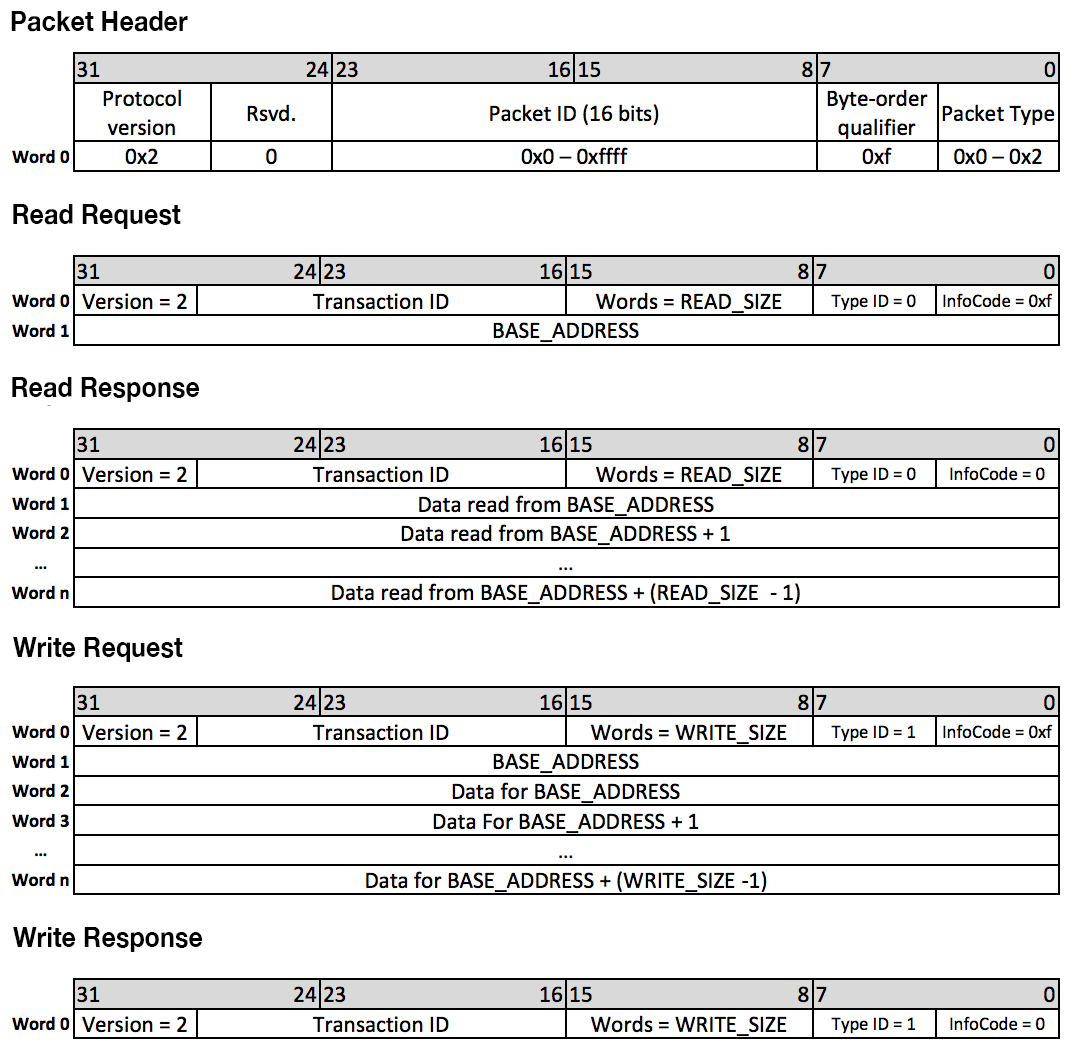
\includegraphics[width=\textwidth]{img/II-2-daq/ipbus.png}
        \caption{??? \cite{AMC13}.}
        \label{fig:II-2-daq-ipbus}
      \end{figure}

      On the electronics side, the IPBus protocol is handled by a master which decodes the requests and forwards it to slaves which each respond to a given address range. Requests involving multiple reads are writes are decomposed by the master in single operations. Slaves receive the request type, address, and data as input parameters and can then treat it as they like. In return, they provide an acknownledgment and optionnally data in the case of a read operation. Eventhough the software treats the address space of 32 bits as a set of read/write registers of 32 bits (A32/D32), the physical implementation on the electronics can be different. Requests can be connected to registers of be used to activate functions on the PCBs. The implementation is up to the developpers.

    \subsection{The XDAQ Application}

  \section{The CSC Data Acquisition System}































-
 % T OK
  %   \cleardoublepage
  %
     % Mieux comparer avec autres tests beam

% Development and Performance of Large Scale Triple GEM for CMS
% Proc. of MPGD2013: 3rd International Conference on Micro-Pattern Gaseous Detectors, 1-4 July, 2013, Zaragoza, Spain; Corr. author: Othmane Bouhali
% A des resultats sur cluster size pion et HV
%

% https://twiki.cern.ch/twiki/pub/CMS/CmsGEMPapers/elba12_colafranceschi_v3.pdf
% has results on HV

% https://twiki.cern.ch/twiki/pub/CMS/CmsGEMPapers/1211.3939.pdf
% Has results on Cluster size

% https://twiki.cern.ch/twiki/pub/CMS/CmsGEMPapers/Michal_COMO_proceeding.pdf
% Has results on cluster size

% https://twiki.cern.ch/twiki/pub/CMS/CmsGEMPapers/TIPP11-D-11-00158.pdf
% HNas resuklts on HV

\chapter{A Data Acquisition System for the Test Beam}
\label{chap:II-3-test-beam}

  During the ongoing process of the development of the DAQ system, the electronics has been tested in two test beams organized in Fall 2014 and November 2015. The first test beam, ran with the first prototype of the DAQ, aimed at proving the feasibility of the architecture of the system, not focusing on data taking from the provided pion and muon beam but rather on usability. As the results were encouraging, the second version of the electronics was developed involving a complete redesign of the hardware, firmware, and software. Therefore, we will mainly focus on the second test beam, which electronics is described in the previous chapter, during which abundant data was recorded showing both excellent results for the detectors and the DAQ system. \\

  In this chapter, we present the firmware and software developments done for the DAQ system for the test beams followed by the analysis of the recorded data. First, we will present the firmware architecture of the OH and the GLIB to better understand the global layout of the system and the features that have been implemented to control the components. Then we will move on to the back-end applications developed to control and monitor the DAQ system and read out data. Finally, after a presentation of the layout of the test beam setup and its characteristics, we will show the results obtained after analysis of the recorded data.

  \section{Architecture of the OptoHybrid Firmware}

    The most important function of the OptoHybrid is to transfer data between the VFAT2s and the GLIB. Downwards, from the off-detector to the on-detector electronics, it transfers slow control requests and fast commands while upwards it sends the trigger and tracking data back to the back-end system. Next to the handling of the basic VFAT2 functionalities, it must also handle the optical links and a couple of programmable registers which control the system. Furthermore, procedures that were previously implemented in software and required extensive computational time have been moved to firmware in order to speed up the system. \\

    Although rather complex, the firmware of the OptoHybrid can be decomposed in six blocks: the fast commands, the trigger data, the tracking data, the slow control, the calibration routines, and the optical links. Even tough these blocks separately will be presented, they are tightly interconnected using a wishbone-like architecture for intercommunication.

    \subsection{Internal Communication Through a Wishbone-Like Bus}

      Wishbone is an open-source communication protocol used in many projects to enable data transfer between ICs. A light version of the protocol has been implemented in the OptoHybrid to link the various modules of the system. The latter are divided in two categories: masters which initiate requests, and slaves which provide responses. The link between the two is done through a switching hub which redirects the requests to the appropriate slaves by using a 32-bit-long address space mapped to the various modules. By design, multiple masters can interact simultaneously with different slaves allowing for parallelism in the system. \\

      A request form a master is composed of four signals: a flag signaling the presence of a request, a write-enable bit to indicate the nature of the request (read or write), a 32-bit-long address to which the request will be redirected, and an optional 32-bit-long data field in case the request is a write operation. The response from a slave consists of: an acknowledgment signal, a 4-bit-long error status in case the operation failed, and an optional 32-bit-long data field holding the response to read requests. A programmable timeout has also been implemented to avoid blocking operation. Some components implement both a master and a slave module in order to be able to receive requests and propagate them to various other modules. \\

      Communication done through the wishbone-like protocol is used mainly for slow control or non-time-critical operations as the latency of a transaction is not fixed. Indeed, the switching hub implements a waiting list functionality which allows two masters to address the same slave at the same time by storing one of the requests in memory and awaiting for the slave to finish the other transaction.

    \subsection{Encoding Fast Commands}

      Fast commands such as L1As, Resyncs, BC0s, etc can originate from various sources. In normal data taking runs, the AMC13 receives the TTC signals, forwards them to the microTCA AMC which in turn transmits them to the OptoHybrid. When data taking is stopped and calibration runs are performed, the routines implemented in the OptoHybrid are ran and require fast commands. To this end, the TTC signals can also be generated locally using the T1 generator block. This entity can generate L1As, Resyncs, BC0s, and CalPulses in three different ways: send a single command a given number of times at fixed interval, send a CalPulse followed by a L1A with a fixed delay, or send a programmable pattern involving all the commands. Finally, the two remaining sources of TTC commands, and more precisly L1As, are either a loopback from a given VFAT2 trigger bits directly to all the VFAT2s (self-triggering) or the signals coming from an external component through a debugging header on the OptoHybrid. \\

      The switching between the various sources is done by setting a register through slow control operations. Once the source has been selected, the commands are forwarded to the VFAT2s and encoded on the T1 signals. Each command is composed of three bits clocked at 40 MHz. An additional feature has been added to the L1A line to throttle the trigger signals when working in high rate environments. Through registers, the operator can select to send only a fraction of the received commands to not overload the VFAT2 buffers and allow for correct readout of the chip.

    \subsection{Formatting Trigger Data}

      Each of the 24 VFAT2s transmits eight trigger bits per BX. These are regrouped using a logic OR in the DAQ system of the test beam  thus yielding 24 bits. The trigger information is used for calibration routines and forwarded over debugging headers to an external electronics crate. As the number of external connections is limited, only six trigger bits can be send thus requiring the need for a selection mechanism controlled by programmable registers.

    \subsection{Acquiring Tracking Data}

      Upon reception of a L1A, the VFAT2 transfers the selected event from its SRAM1 to SRAM2 and then to an encoder which serializes the data. Each event is 192 bits long followed by two idle bits and clocked at 40 MHz. This means that it takes 194 BXs to read out one event and that the VFAT2 cannot handle trigger rates higher than $\approx$ 200 kHz without experiencing an overflow of the buffers. The data is pushed out of the VFAT2 automatically and formatted according to the pattern shown in Table \ref{tab:II-3-vfat2-tk-format}. The top left bits are the Most Significant Bits (MSBs) which are pushed out first and the bottom right bits or the Least Significant Bits (LSBs) which come in last. The first four bits of the first three 16-bit-long words are constant values. These are completed by the BC which increments at each clock cycle, the EC which counts the number of received L1As, four flags which hold information on the status of the buffers, and a chip ID unique to each VFAT2. Following are the 128 bits reflecting the hit information on each channel. Finally, the VFAT2 uses a Cyclic Redundancy Check (CRC) on 16 bits to detect errors. The CRC uses all other 176 bits to encode its data but does not provide a way to correct errors. \\

      \begin{table}
        \begin{tabularx}{\textwidth}{C{1}}
          \textbf{VFAT2 tracking data} \\
          {
          \begin{tabularx}{0.5\textwidth}{|C{1}|C{1}|C{1}|}
            \hline
            \multicolumn{3}{|c|}{15 \hfill 0} \\ \hline
            1010 & \multicolumn{2}{|c|}{BC[11:0]} \\ \hline
            1100 & EC[7:0] & Flags[3:0] \\ \hline
            1110 & \multicolumn{2}{|c|}{Chip ID[11:0]} \\ \hline
            \multicolumn{3}{|c|}{Channel data x8} \\ \hline
            \multicolumn{3}{|c|}{CRC} \\ \hline
          \end{tabularx} }
        \end{tabularx}
        \caption{Format of the tracking data packets sent by the VFAT2s.}
        \label{tab:II-3-vfat2-tk-format}
      \end{table}

      Next to the data line, each VFAT2 provides a DataValid line which is pulled high when the bits coming out of the VFAT2 are valid. However, due to the limited number of pins connecting the GEB and the OptoHybrid, this signal has been left unconnected for all but six VFAT2s. Therefore, data is constantly shifted in a 194 bits (192 bits of data and 2 idle bits) serial-to-parallel converter and analyzed. When the fixed pattern of 12 bits is seen, a flag is raised signaling the presence of potential data. The data packet is split up in its various elements and the CRC is recomputed and compared against the received CRC. Two additional flags respectively hold the results of the comparison of both CRCs indicating if the data is valid or not, and a logic OR of all 128 channel to indicate if the packet contains a hit or not. In theory, only packets with valid CRCs could be transmitted to the back-end electronics. However, sending all packets offers the possibility to identify recurring errors in the CRCs computation and the possibility to correct them offline. \\

      In parallel to the decoding of the data packets, the OptoHybrid maintains its own BC and stores the value of the counter in a buffer each time a L1A is received. When the decoding modules report they have detected data, a concentrator module aggregates the information from all available VFAT2s. Every packet received within a window of 10 BX is assigned to the same event to which the value of the corresponding BC is appended. The assembled event is stored in a large buffer to be latter sent over the optical links to the GLIB. \\

      To prevent positions either not equipped with VFAT2 Hybrids or that are noisy to generate fake data, a 24-bit-long register allows to mask individual positions to ignore any packets it generates. Next to this, each decoding module is equipped with two counters respectively counting the number of valid and invalid packets.

    \subsection{Controlling and Monitoring the Systems}

      The OptoHybrid is used to control itself through wishbone and the VFAT2s through I2C. The slow control of the OptoHybrid mainly consists in selecting TTC command sources, setting the trigger throttling, reading out counters, etc. These operations are performed to control the data flow and the functioning of the DAQ system itself. Commands sent to the VFAT2s on the other hand have direct impact on the physics of the data taking through the bias of the analog front-end readout. \\

      To communicate with the VFAT2s, six I2C controllers are implemented in the firmware of the OptoHybrid, one per sector on the GEB. Each controller can access four VFAT2s which are identified using three resistors that can be installed on the GEB. VFAT2 uses a modified I2C protocol with the same frame format as the official one but a different addressing scheme. The official I2C data frame is shown in Figure \ref{fig:II-3-i2c}. The master starts by sending seven address bits which are used to identify the slave it wants to talk to, followed by a read/write bit. After the slave acknowledged the request, eight bits are sent from the master to the slave in case of a write operation followed by a slave acknowledgment, or the opposite in case of a read operation. For the VFAT2, the first three bits of the address are used to select the chip that is addressed by the master while the four remaining bits are used to select the register that needs to be accessed. This addressing scheme allows the OptoHybrid to access up to 16 registers on the VFAT2s. However, each VFAT2 holds 16 primary registers and 136 extended registers. The extended registers are accesses using two primary pointer registers: one set to point to an extended register, and one to read/write the data in said register. Thus, in order to perform a transaction on a primary register, only one operation is necessary, while two are required to access extended registers. \\

      \begin{figure}[h!]
        \centering
        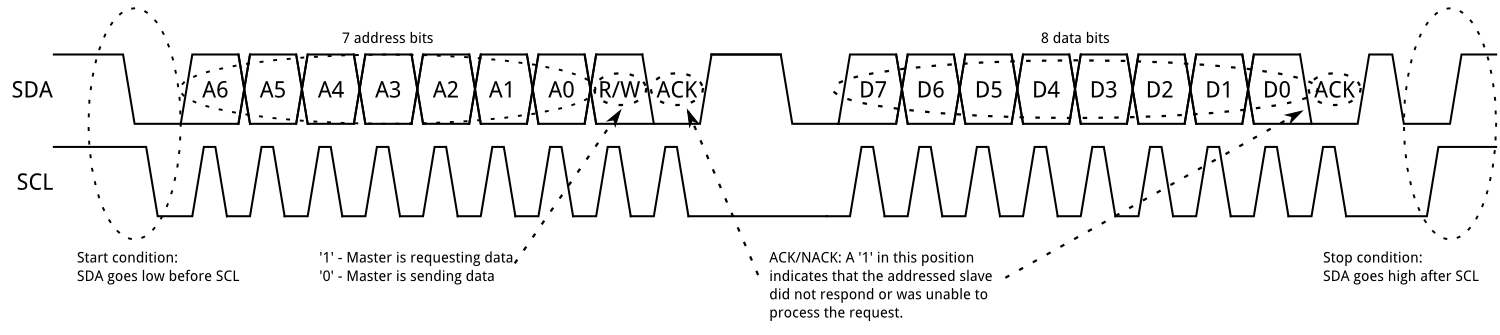
\includegraphics[width=\textwidth]{img/II-3-test-beam/i2c.png}
        \caption{Data format of an I2C communication \cite{I2C}.}
        \label{fig:II-3-i2c}
      \end{figure}

      To make this process transparent to the user and flatten out the address space of the VFAT2s, the OptoHybrid maps the primary registers from addresses 0 to 16 and the extended registers from addresses 17 to 152. When performing a transaction with the extended registers, the I2C controllers automatically run the double addressing scheme. \\

      Next to the basic I2C controllers, an extended I2C controller was developed to abstract individual addressing and allow request broadcasting. This module forwards I2C requests to all selected VFAT2s at once to configure the entire system in parallel. A programmable register allows to leave out given VFAT2s from the broadcast while a buffer stores the result of the operations.

    \subsection{Calibrating the Systems}

      The calibration routines have been ported from software to firmware in order to increase their speed of operation and reduce the number of requests that need to be performed. The routines are as follows: a threshold scan which measures the noise on the channels as a function of the threshold of the VFAT2s, a latency scan which allows to select the correct BX when receiving L1As, and a s-curve scan which characterize the response of the channels as a function of the collected charge and threshold. \\

      \paragraph{The threshold scan} is used to scan each VFAT2 for noise. For each threshold value set on the VFAT2, the percentage of events displaying a hit is recorded and taken as the percentage of noise. A graph can be obtained showing the noise decrease as the threshold increases yielding a point at which the system can be operated with minimal noise. The threshold scan can be operated using trigger information or the 128 channels as a whole, or on individual channels using tracking data. For the latter, the T1 generator is used as trigger source to generate data as these runs are being performed when the beam is off. No relation between a L1A and physical event is needed to study the noise on the system. \\

      \paragraph{The latency scan} allows to determine the best latency value to be set in a VFAT2. The latency is the time difference, in number of BX, between the time of arrival of a L1A and the time at which the related event was stored in the VFAT2 buffer. This module is operated when the particle beam is on and triggers are generated by an external source such as a Photomultiplier (PM) placed in front of the detector. For each value of the latency, the OptoHybrid counts the ratio of events with hits over the total number of events. For a noiseless VFAT2 with 100\% detection efficiency, the ratio would be 0\% outside the correct latency window and 100\% inside. The size of the window can be adjusted by changing the length of the monostables output in the VFAT2s. \\

      \paragraph{The s-curve scan} is part of the calibration routines performed for the qualification of the VFAT2s. It yields the response of the VFAT2 channels to an injected charge pulse according to the threshold. It is used in conjunction with the T1 generator which send a CalPulse followed by a L1A at fixed interval, thus with known latency. The use and results obtained for this module are further detailed in Chapter \ref{chap:II-4-qualification}.

    \subsection{Optical Communication with the Off-Detector Electronics}

      The connection between the OptoHybrid and the off-detector electronics is the optical links from which two are used: one for the trigger data and fast commands, and one for the tracking data and slow control. Each optical fiber is connected to an SFP+ transceiver which contains the Light Emitting Diode (LED) that drives the link. The SFP+ module is in turn connected to a Gigabit Transceiver X (GTX) block inside the FPGA which is a dedicated component that can handle high-speed serial communications.

      \paragraph{The GTX module} is in charge of the serialization/deserialization of high-speed data. A schematic diagram of the functions it provides is shown in Figure \ref{fig:II-3-gtx}. The GTX handles both the transmission and reception of data. From the FPGA logic, it receives a parallel vector of bits containing the raw data. The raw data enters the Transmit FIFO which acts as a buffer before the Line Encoding module. The latter uses an eight-bit/ten-bit (8b/10b) encoding scheming which is a standard in high-speed communications. 8b/10b encodes every eight bit word on ten bits according to a predefined table. It has the particularity that whatever combination of words might be sent, no more than five successive '0's or '1's will arise in the serial stream. This ensures line balancing: the fact that the electric lines between the GTX and the SFP+ module will remain at an average voltage and not drift to a logic '1' or '0' over time, thus requiring a longer fall or rise time of the signals. 8b/10b also offers a set of K-characters which are unique patterns of bit that can never arise randomly in the stream. Those characters are used to detect the beginning of a frame and allow the receiver to align correctly. Finally, after the encoding of the data frame is done, it is serialized and transmitted to the SFP+ module over differential pairs. \\

      \begin{figure}[h!]
        \centering
        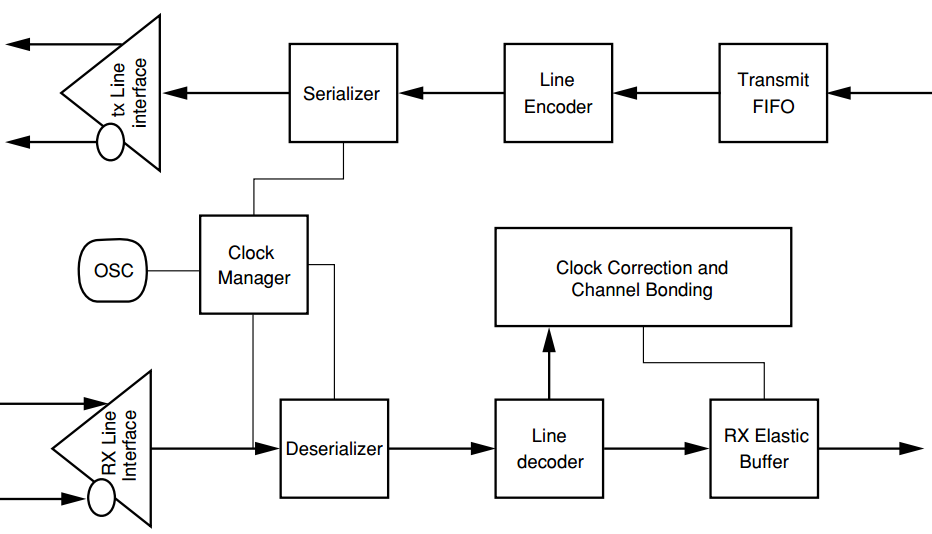
\includegraphics[width=\textwidth]{img/II-3-test-beam/gtx.png}
        \caption{Functionnal diagram of the Gigabit Transceiver X module used inside the Xilinx Virtex-6 FPGAs for high-speed serial communication \cite{GTX}.}
        \label{fig:II-3-gtx}
      \end{figure}

      The receiver essentially follows the opposite path as the transmitter except for the Clock Management block. The 8b/10b encoding offers one more advantage which is the possibility to recover a clock from the data stream itself, technique called Clock Data Recovery (CDR). In high-speed signal design, small variations in the clock frequency between the transmitter and the receiver can lead to discrepancy in the read out data. To avoid this, the receiver can tune the frequency of the clock of its deserializer using the transitions of the bits in the incoming stream to align its phase to the data. The GTX block further provides the obtained recovered clock to the FPGA to use in the logic. Correct alignment of the data is checked using the K-characters in the stream.

      \paragraph{The fixed latency link} is used to transmit trigger data from the OptoHybrid to the GLIB and receive the fast commands. Of the 64 bits that the downlink transmits every BX, 16 are used to align the serial bit stream on the receiving side and four others are used to encode the four fast commands that the VFAT2 understands. The other 44 bits are not used and left to constant zeros. The uplink uses a 16 bit header to align the stream to which it appends the 24 triggers bits coming from the logic-OR of the VFAT2s. These patterns repeat at 40 MHz as data changes every BX.

      \paragraph{The variable latency link} is used to transmit and receive slow control commands and to transmit the tracking data of one VFAT2 at the time to the GLIB. As only one VFAT2 was exposed to the beam at any given time during the test beam, reconstructing and sending the full event was not a necessity for the DAQ system. In both directions, a given frame format is constantly sent using two bits in the header to indicate the presence of a valid slow control request and valid VFAT2 tracking data in case of the uplink. The two data formats are shown in Table \ref{tab:II-3-data-format}. Both send a 16 bit header to align the link followed by the frame data. As can be seen in the table on the left, the OptoHybrid receives requests from the optical link which are then converted to wishbone-like requests by the logic. The optical link module is one of the wishbone masters that controls the system and which responses are forwarded back to the GLIB.

      \begin{table}
        \begin{tabularx}{\textwidth}{C{1}C{1}}
          \textbf{GLIB to OptoHybrid frame} & \textbf{OptoHybrid to GLIB frame} \\
          {
          \begin{tabularx}{0.4\textwidth}{|C{1}|}
            \hline
            15 \hfill 0 \\ \hline
            Header \\ \hline
            Request address (MSB) \\ \hline
            Request address (LSB) \\ \hline
            Request data (MSB) \\ \hline
            Request data (LSB) \\ \hline
            CRC \\ \hline
          \end{tabularx} }
          &
          { \begin{tabularx}{0.4\textwidth}{|C{1}|}
            \hline
            15 \hfill 0 \\ \hline
            Header \\ \hline
            VFAT2 data x14 \\ \hline
            Response data (MSB) \\ \hline
            Response data (LSB) \\ \hline
            CRC \\ \hline
          \end{tabularx} }
        \end{tabularx}
        \caption{Format of the data packets used to communicate between the GLIB and OptoHybrid.}
        \label{tab:II-3-data-format}
      \end{table}

    \subsection{System Summary}

      The aim of the OptoHybrid firmware is to provide a communication medium between the VFAT2s and the off-detector electronics and to speed up the calibration routines by implementing them closer to the detector. The developments that have been listed in this chapter are targeted at the OptoHybrid v2a and the configuration of the system ran during the test beams. Modifications have to be brought for the final system although the foundations of the firmware have been solidly laight out.

  \section{Architecture of the GLIB Firmware}

    The GLIB development group at CERN provides a system firmware which controls the on-board components, handles the communication with the MCH, and implements the logic to decode IPBus requests. This code is similar to the operating system in which the users runs their applications by adding custom firmware. The latter is system specific and up to the user to develop. In this application, the firmware developed for the GLIB is in charge of the buffering of the tracking data until it is read out by the application, and the forwarding of the IPBus requests over the optical link to the OptoHybrid. Other than that, the GLIB holds a couple of counters which monitor the status of the optical links and the number of requests performed. However, the firmware of the GLIB has been designed to be able to handle two OptoHybrids in parallel, seamlessly allowing the user to switch from one to another at any time.

    \subsection{The Tracking Data Readout}

      The GLIB acts as buffer for the tracking data it reads out from the OptoHybrids and decodes from the optical links. It stores the VFAT2 events until the control and monitoring application reads them out through IPBus. In case the buffers reach their full occupancy, new events are discarded and flags are raised. The buffers can hold up to 16,383 VFAT2 events per OptoHybrid connected and the system has been tested and proven to work without overflows up until L1A rates of 200 kHz, the maximum rate the VFAT2s can handle.

    \subsection{The IPBus Controller and Slaves}

      The IPBus decoding procedure is similar to the wishbone system implemented on the OptoHybrid. According to the address contained in the request, the GLIB selects the slave it needs to address. Each request is made of a flag signaling the presence of a request, a read/write bit reporting the type of operation, a 32-bit-long address field, and an optional 32-bit-long data field populated with data in case of a write operation. The IPBus response is composed of an acknowledgment and error flag to signal the validity of a response, and an optional 32-bit-long data field containing the read data. By design, each IPBus request is decomposed in single read or write operations. Therefore, even if the software performs a read request of multiple addresses at once, IPBus slaves will still see this as multiple sequential read operations on single addresses. This in term propagates to the OptoHybrid wishbone requests which originate from IPBus, meaning that no more than one operation coming from the GLIB is present at any time in the system. As a majority of the requests have to be forwarded to the OptoHybrid, an entire address space of the GLIB is mapped to the former. These are handled by an IPBus slave connected to the GTX blocks of the GLIB. This module encodes the request according to the data format on the left in Table \ref{tab:II-3-data-format} and awaits for a response before signaling the IPBus controller.

  \section{The Control and Monitoring Application}

    The first version of the control and monitoring application that communicated with the system was based on a series of Python scripts running PyChips, a Python implementation of IPBus provided with the GLIB source code. Each script was developed to run a specific task and needed to be ran over and over again. This was feasible for the first test beam during which only the system was tested for small amounts of time, but not for the second one that was ment to collect data. Therefore, a web application was developed based on NodeJS \cite{NODEJS} as server technology, SocketIO \cite{SOCKETIO} for the client/server exchange, AngularJS \cite{ANGULARJS} as front-end framework, and Bootstrap \cite{BOOTSTRAP} as design framework.

    \subsection{Architecture of the Application}

      NodeJS is a JavaScript (JS) runtime that has the ability to run JS code outside the context of a web browser. It extends JavaScript from its original use in web content to a wide range of applications by enabling it to manipulate files, data streams, etc. The most common use for NodeJS is the implementation of a web server that has the property to be much more reactive than other infrastructures. Where classic server structures display a blocking behavior, meaning they only handle one request at the time blocking the queue of incoming demands, NodeJS is event driven and thus non-blocking. For example, if a client requests a file, NodeJS will transfer the request to the operating system and continue to respond to other client as long as the file is not served. Interactions are thus more reactive and allow to easily implement a real-time control and monitoring system. Along side the NodeJS server that serves the content of the web application, a version of IPBus in JS was also implemented. The latter allows the server to execute IPBus requests on the GLIB and readout the response. \\

      To link the client side controlled by the user and the server side which sends requests to the GLIB, the SocketIO project is used. It is an abstraction layer on the fairly new WebSocket technology which adds sockets to web browsers and allows for fast communication with servers by bypassing the HTTP protocol. When the client changes settings in its web browser, SocketIO transfers the request to NodeJS which in turn creates an IPBus packet. When the GLIB responded to the request, the server transfers the response back to the client which can handle the data as it likes. \\

      To handle data in a dynamic and convenient way, the web pages use Bootstrap and AngularJS. Bootstrap is a design framework which provides simple and readable themes to layout the pages. The content of the page on the other hand is managed by AngularJS which is a front-end JS framework. It helps rendering dynamic content in function of the data received from the server. Actions can be triggered or disabled according to the state of the system, data can be updated live, etc. It renders the user experience more fluid and enjoyable by providing a usable set of actions and an efficient navigation through the control pages.

    \subsection{Controlling the Systems}

      The control over the GLIB, OptoHybrids, and VFAT2s is done through four pages, which screenshots are shown in Figure \ref{fig:II-3-app-monitoring}. The top-left picture displays the home page of the application which provides an overview of the status of each system. The left panel displays the firmware version of the GLIB and OptoHybrid; the middle panel gives the occupancy of the GLIB readout buffers, which are here signaled as full through the use of a red flag, and the status of the various modules of the OptoHybrid; finally, the right panel lists the VFAT2s that are turned on in green, turned off in red, and missing in gray. By clicking on any of the elements, the user is redirected to the corresponding system control page. \\

      \begin{figure}[h!]
        \centering
        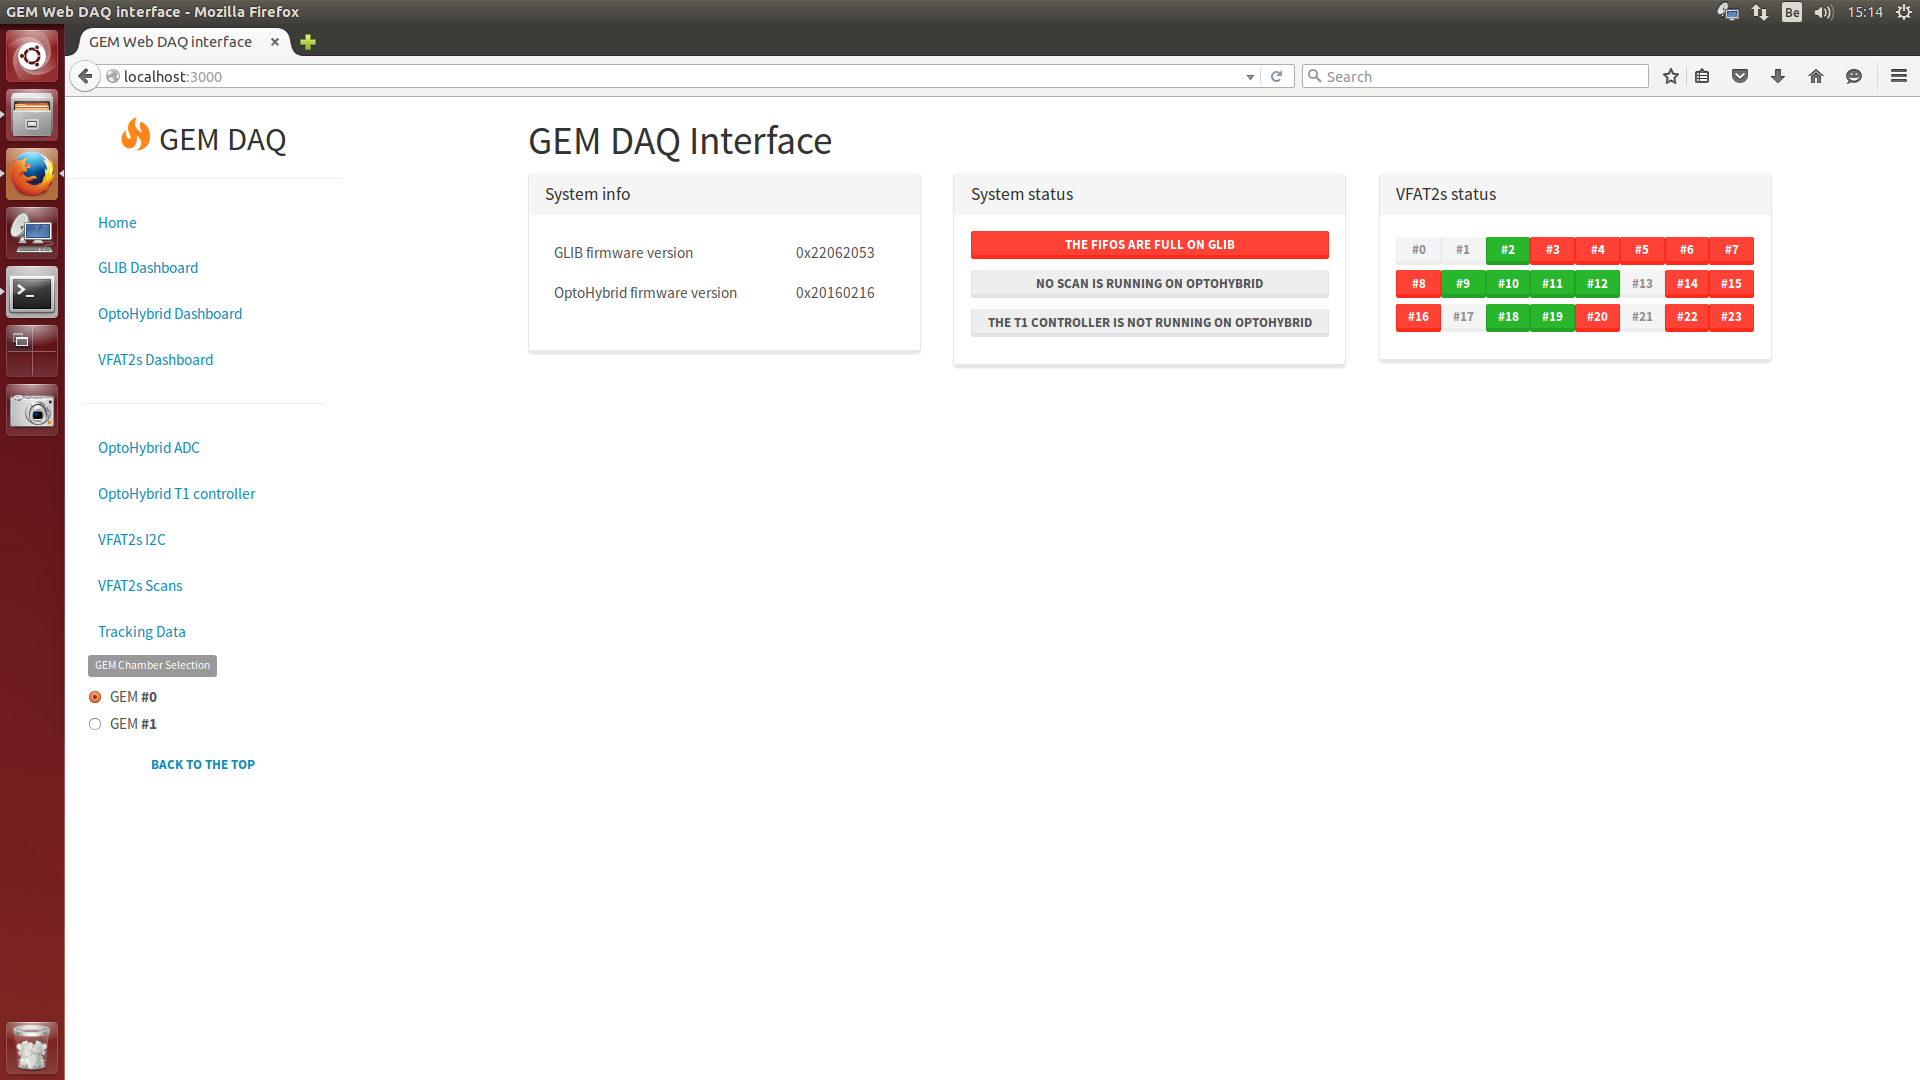
\includegraphics[width=0.49\textwidth]{img/II-3-test-beam/app-home.png}
        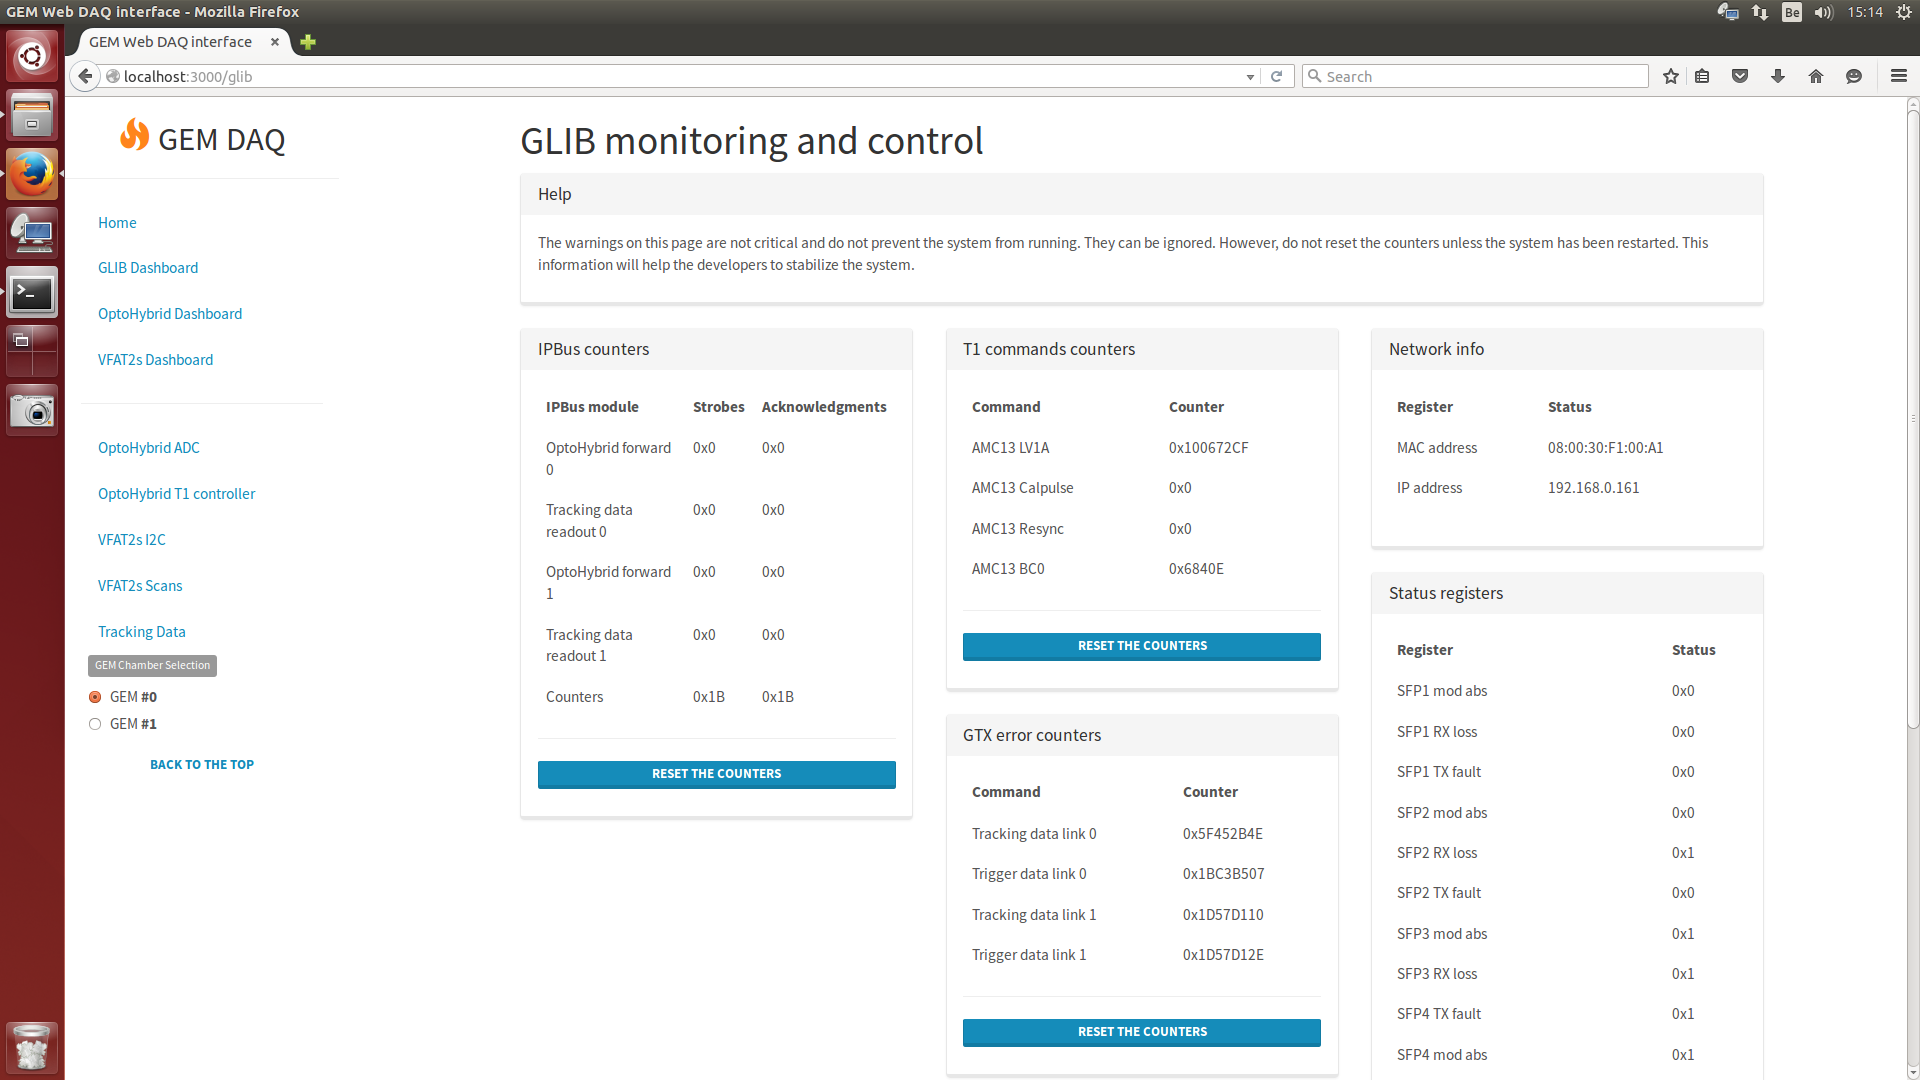
\includegraphics[width=0.49\textwidth]{img/II-3-test-beam/app-glib.png} \\
        \vspace*{0.3cm}
        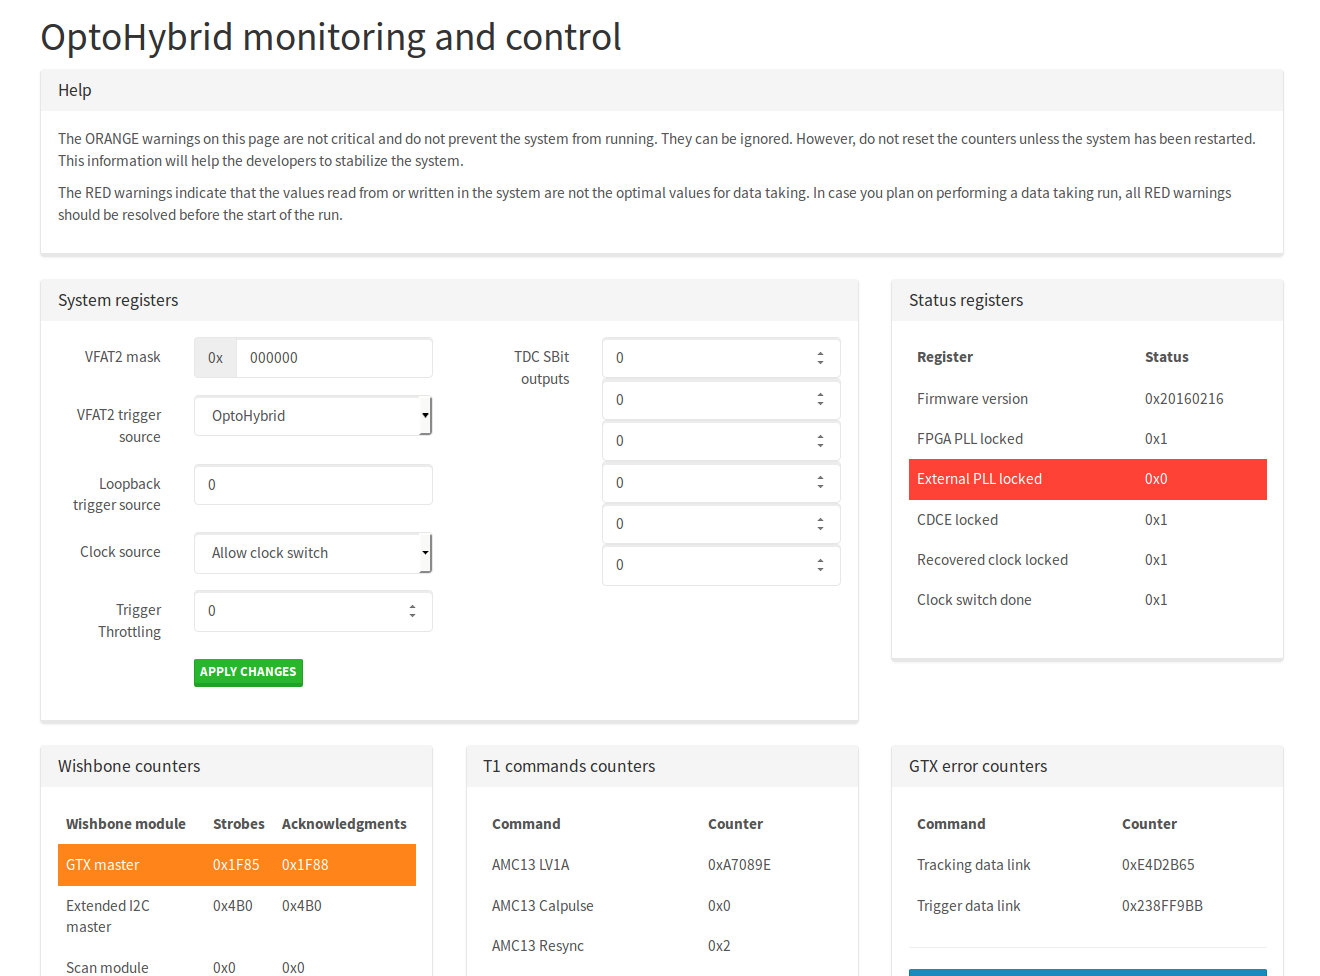
\includegraphics[width=0.49\textwidth]{img/II-3-test-beam/app-oh.png}
        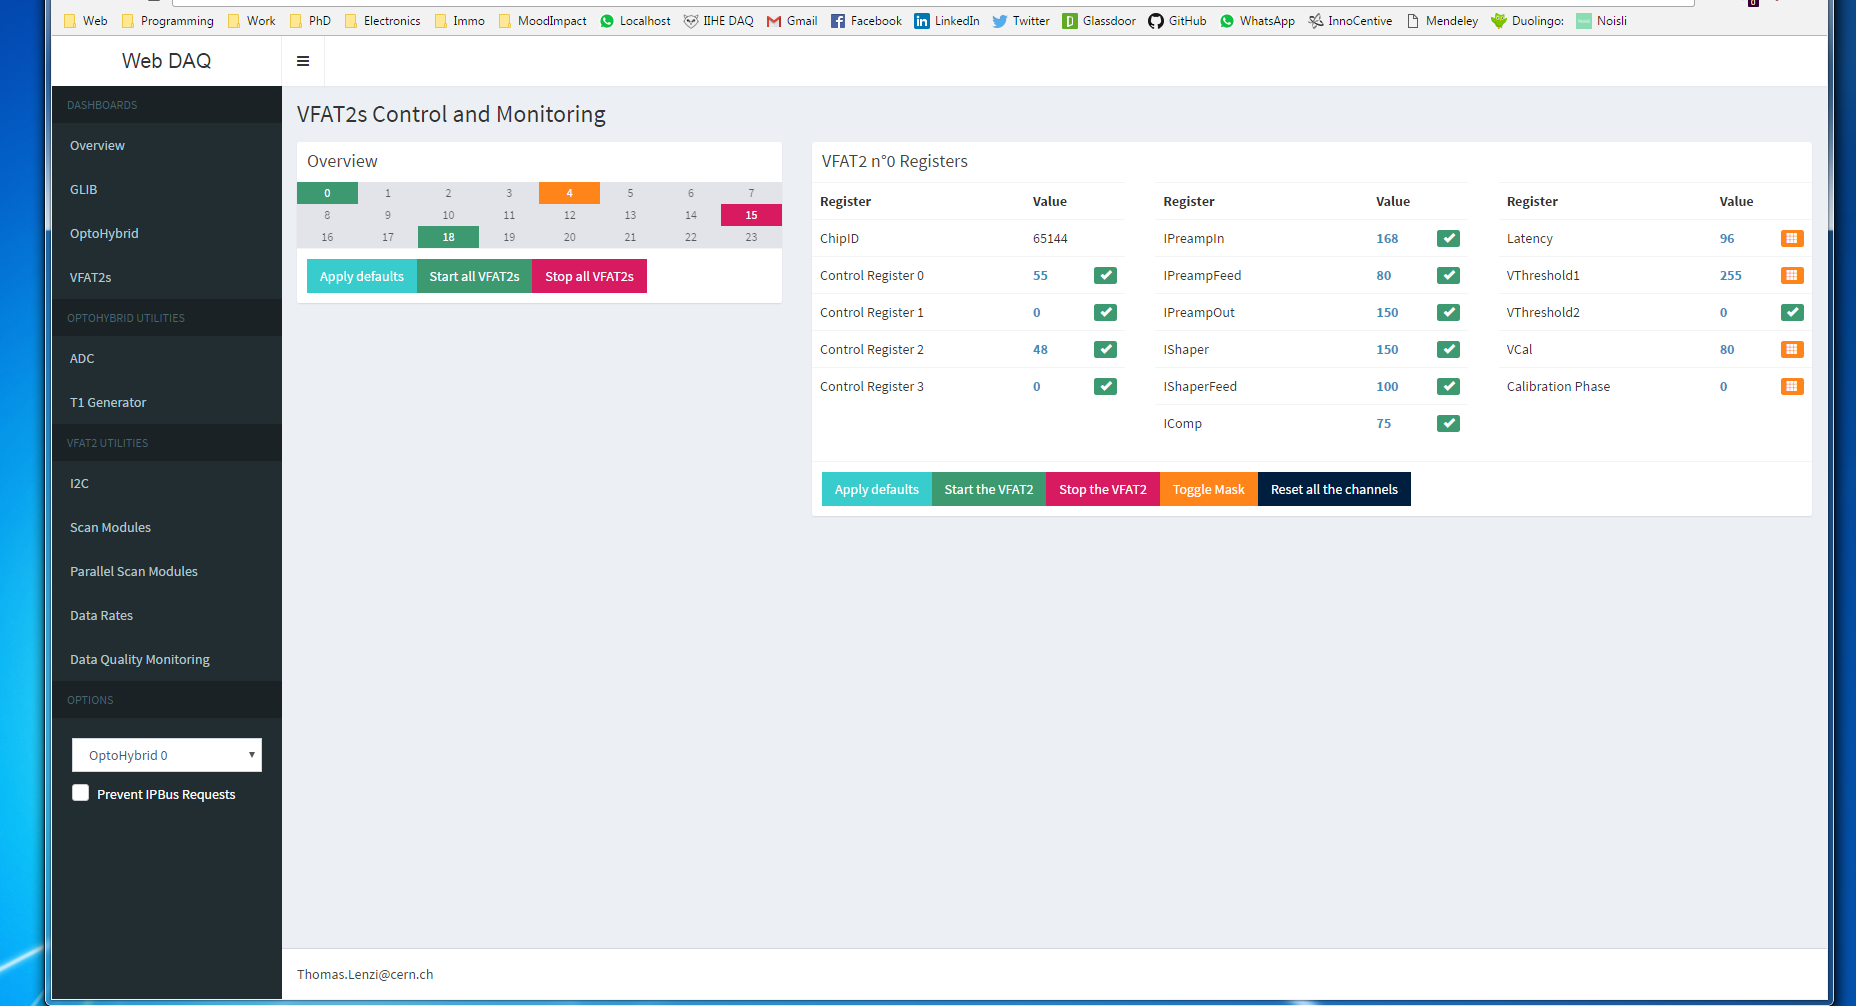
\includegraphics[width=0.49\textwidth]{img/II-3-test-beam/app-vfat2.png}
        \caption{Screenshots of the web application used to control and monitor the components of the DAQ system.}
        \label{fig:II-3-app-monitoring}
      \end{figure}

      The control page of the GLIB is shown in the top-right corner. The information it contains is mainly related to counters which allow to see, for example, the number of requests sent to the OptoHybrid and the number of responds received. It also counts the number of errors detected on the optical link providing a quantitative value of the health of the link. \\

      The OptoHybrid page, shown in the bottom-left corner, provides more information and control options to the user. The top-left part of the page is used to modify system register controlling the trigger source, clock source, trigger information sent over the debugging header, etc. This is where the user can change the type of ongoing run by going from a data taking run using external triggers to a calibration run using internally generated triggers. The panel directly on the right provides status information on the various clocking resources in the FPGA. By default, the OptoHybrid uses the on-board oscillator to power the system and the optical links. As communication is established with the GLIB, the GTXs provide the recovered clock from the link which is the system clock. When the latter is stable, the OptoHybrid can decide to switch from its on-board clock to the system clock in order to be synchronous with the whole DAQ system. This operation can be prohibited, forced, or allowed by the user, which can also chose to use an external clock provided through the debugging header. These clocking options are useful for the test beam setup where the clock can be provided externally to synchronize with other electronics equipment. Finally, the bottom part of the page display counter values for the wishbone request, fast commands, link errors, etc. Note that when a discrepancy is observed between two correlated counters, a warning flag is raised as can be seen in the bottom-left of the picture. \\

      Finally, the control page of the VFAT2s, shown in the bottom-right of the figure, gives access to the most significant registers of the front-end chips. It provides a summary of the on/off/absent status of each VFAT2 on the GEB and, by clicking on an individual slot, the value of each register as shown in the panel on the right. Default settings for the registers are saved in memory and compared to the current values, raising warnings when they differ and allowing the user to correct them. The user can also control all the VFAT2s at once by applying the default settings or turning them on or off at the same time. In the bottom panel, control buttons allow to mask individual VFAT2s in case they generate noise or send corrupted tracking data. Two counters monitor the number of valid (with a correct CRC) and invalid packets each position has sent.

    \subsection{Fast and Slow Control of the VFAT2s}

      The fast control or T1 generator is controlled by a dedicated page, displayed in the left of Figure \ref{fig:II-3-app-control}, which allows to select the type of commands to generate, the pattern to send, and the delay between two pulse. The slow control of the VFAT2s handled by the I2C modules and the extended I2C controller is managed by another page shown in the right. The slow control commands can either target a single VFAT2 as shown in the left panel or an entire set of chips as can be seen in the right panel. In case of a single command, the response is shown inline. For multiple operations, a table of results is shown indicating the value and the corresponding VFAT2. To help the user, the accessible registers are named rather than listed using their address.

      \begin{figure}[h!]
        \centering
        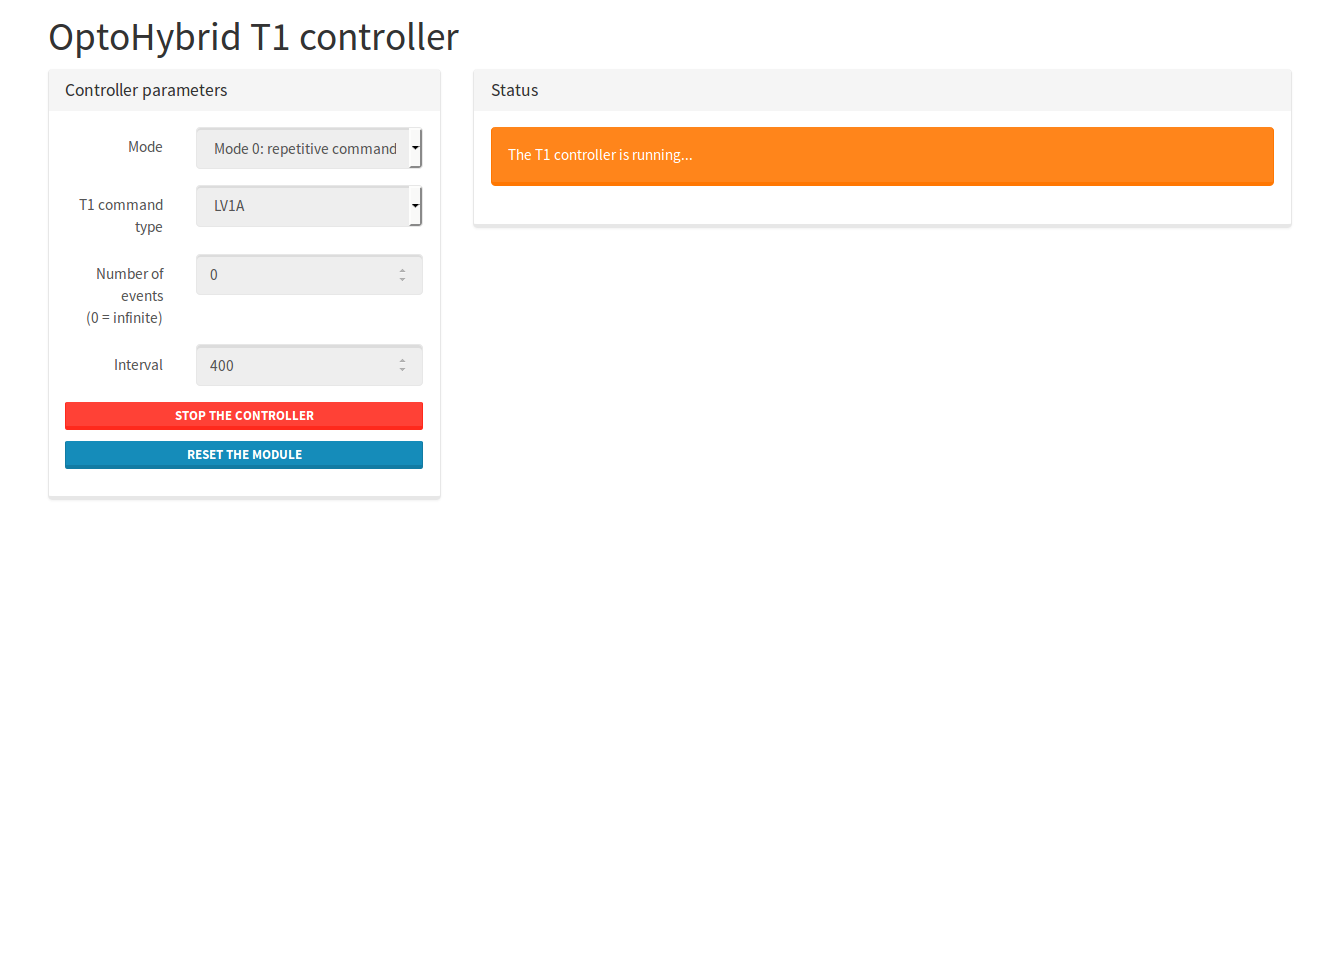
\includegraphics[width=0.49\textwidth]{img/II-3-test-beam/app-t1.png}
        \includegraphics[width=0.49\textwidth]{img/II-3-test-beam/app-i2c.png}
        \caption{Screenshots of the pages of the web application used to send fast commands (left) and slow control (right) requests to the VFAT2s.}
        \label{fig:II-3-app-control}
      \end{figure}

    \subsection{Calibrating the VFAT2s}

      The calibration of the VFAT2s is done through a dedicated page which regroups the various operations that can be performed on the chip. Figure \ref{fig:II-3-app-calibration} is a screenshot of the application running a threshold scan on one of the VFAT2s. The left panel allows the user to select all the required parameters such as the type of scan, the range of the scan, the number of events per point, etc. Once the parameters are entered, the user starts the scan and waits for it to finish in firmware. When done, a graph displays the results in the right panel. The user can than dynamically change VFAT2 settings by clicking on a point of the graph to, for example, select the most appropriate threshold or latency value. Furthermore, the user can save the data points to disk for offline analysis.

      \begin{figure}[h!]
        \centering
        \includegraphics[width=\textwidth]{img/II-3-test-beam/app-scan.png}
        \caption{Screenshot of the page of the web application used to perform calibration scans of the VFAT2s.}
        \label{fig:II-3-app-calibration}
      \end{figure}

    \subsection{Data Quality Monitoring}

      DQM is used online to check the consistency of data recorded. This is the last component of the application shown in Figure \ref{fig:II-3-app-tk}. This page monitors the status of the readout buffers of the GLIB and allows the user to acquire data. Once acquisition has started, plots begin to fill with the various parameters extracted from the VFAT2 data format. The user can visualize the number of data packets, BC, EC, flags, and chip ID distribution, the occupancy of the channels, etc, effectively monitoring the validity of the data and if required change the parameters of the run. Although this application has the ability to readout data and store it to disk, this feature was not used to this intend during the test beam. A XDAQ based program developed by the software development team of the GEM collaboration was used to acquire raw data from the GLIB and store it on disk in text files for later analysis.

      \begin{figure}[h!]
        \centering
        \includegraphics[width=\textwidth]{img/II-3-test-beam/app-tk.png}
        \caption{Screenshot of the page of the web application used to do online data quality monitoring.}
        \caption{???}
        \label{fig:II-3-app-tk}
      \end{figure}

  \section{The Test Beam Setup}

    The test beam campaigns took place at CERN in the North Area of Prevessin, one of the secondary sites. The beam provided to the experiments originates from the SPS proton bunches which are extracted from the accelerator at 400 GeV and interact with four primary targets (T2, T4, T6, and T10) to produce the secondary beams mainly composed of electrons and hadrons. A selection on the type of particles and their momentum is performed and the beam is guided towards the experimental setups, namely H2 and H4, using dipole magnets. In the transfer tunnels, collimators can be adjusted to increase or reduce the flux of particles and an optional secondary target can be placed in the beam path to create a tertiary beam. Figure \ref{fig:II-3-sps} shows the monitoring page of the SPS indicating the presence of spills of particles in yellow. Spills last between 4.8 s and 9.6 s and repeat every 14 s to 48 s depending on the SPS operation. \\

    \begin{figure}[h!]
      \centering
      \includegraphics[width=0.8\textwidth]{img/II-3-test-beam/sps.png}
      \caption{Monitoring page of the SPS indicating the presence of spills of particles (yellow).}
      \label{fig:II-3-sps}
    \end{figure}

    The two types of particles used during the test beam were pions and muons. Pions are obtained from the secondary beam by inserting a thin absorber which removes the electronic component of the beam. They can reach intensities between 10$^4$ and 10$^7$ particles per spill and produce a very narrow beam. From their decay, a muon beam can be obtained by using moderate intensity secondary beams and closing the collimators. The muon beam reaching the experimental setup is a wider and less intense.

    \subsection{The GEM Detectors Setup}

      During the November 2015 test beam campaign, a superchamber of GE1/1-V detectors has been used to collect data. Each detector was equipped with 12 VFAT2 Hybrids mounted in the central four rows. The remaining slots, too far away from the beam spot, were covered with grounding equipment to reduce noise. Each GEM was mounted with a GEB v2 and a OptoHybrid v2a. A picture of the setup is shown in Figure \ref{fig:II-3-test-geb}. Both OptoHybrids were connected to the same GLIB placed in a microTCA crate. \\

      \begin{figure}[p!]
        \centering
        \includegraphics[width=\textwidth]{img/II-3-test-beam/test-geb.jpg}
        \caption{Photograph of the GEM detectors used during the test beam and equipped with the full DAQ system.}
        \label{fig:II-3-test-geb}
      \end{figure}

      The GEM detectors were connected to a gas system providing a mixture of Ar/CO$_2$/CF$_4$ at 45\%, 15\%, and 40\% respectively. The high-voltage was delivered through a ceramic high-voltage divider for one chamber and by separate channels connected directly to the GEM foils and planes for the other. The high-voltage applied is expressed in terms of current flowing through the divider which, by summing up the individual resistors that it is made of, yields a value in volts. Table \ref{tab:II-3-test-hv} enumerates the different values of the voltages according to the current flowing through the divider. The difference between the divider and drift plane values is due to an input filter placed before the latter which smooths out fluctuations in the voltage. The low voltages for the OptoHybrids (1.8 V and 4 V) and for the GEBs (2.5 V) were delivered by two power boards mounted on top of the detector stand, along with the necessary tools to reprogram the FPGA in case of failure and the debugging headers.

      \begin{table}[h!]
        { \footnotesize
        \begin{tabularx}{\textwidth}{|C{1}|C{1}|C{1}|C{1}|C{1}|C{1}|C{1}|C{1}|C{1}|}
          \hline \textbf{Current ($\mu$A)} & \textbf{Divider (V)} & \textbf{Drift plane (V)} & \textbf{GEM1 top (V)} & \textbf{GEM1 bottom (V)} & \textbf{GEM2 top (V)} & \textbf{GEM2 bottom (V)} & \textbf{GEM3 top (V)} & \textbf{GEM3 bottom (V)} \\ \hline
          700 & 3921 & 3290 & 2503 & 2107 & 1801 & 1416 & 805 & 437 \\
          710 & 3977 & 3337 & 2538 & 2137 & 1827 & 1437 & 816 & 443 \\
          720 & 4033 & 3384 & 2574 & 2167 & 1853 & 1457 & 828 & 450 \\
          730 & 4089 & 3431 & 2610 & 2198 & 1879 & 1477 & 839 & 456 \\
          740 & 4145 & 3478 & 2646 & 2228 & 1904 & 1497 & 851 & 462 \\
          750 & 4201 & 3525 & 2682 & 2258 & 1930 & 1518 & 862 & 468  \\
          760 & 4257 & 3572 & 2717 & 2288 & 1956 & 1538 & 874 & 475 \\
          770 & 4313 & 3619 & 2753 & 2318 & 1981 & 1558 & 885 & 481 \\
          780 & 4369 & 3666 & 2789 & 2348 & 2007 & 1578 & 897 & 487 \\
          790 & 4425 & 3713 & 2825 & 2378 & 2033 & 1598 & 908 & 493 \\
          800 & 4481 & 3760 & 2860 & 2408 & 2059 & 1619 & 820 & 500 \\
          810 & 4537 & 3807 & 2896 & 2438 & 2084 & 1639 & 931 & 506 \\ \hline
        \end{tabularx}
        }
        \caption{Values of the voltages applied to the detectors according to the current flowing through the high voltage resistive divider.}
        \label{tab:II-3-test-hv}
      \end{table}

    \subsection{The Beam Area Setup}

      The GE1/1 superchamber was inserted in the beam path and adjusted so that solely one VFAT2 in the middle column would be exposed to the beam spot. Figure \ref{fig:II-3-test-setup} shows the setup on the left placed in front of the beam transfer tunnel on the right side. Four scintillators, three placed in front of the detector and visible in the picture, and one placed in the back of the detector were used to provide triggers to the system. The output of the four scintillators was converted to Nuclear Instrumentation Module (NIM) logic and their coincidence used as the trigger source of the system. \\

      \begin{sidewaysfigure}[p!]
        \centering
        \includegraphics[width=0.9\textwidth]{img/II-3-test-beam/test-setup.jpg}
        \caption{Photograph of the two detectors on the left placed in front of the beam transfer tunnel on the right side.}
        \label{fig:II-3-test-setup}
      \end{sidewaysfigure}

      NIM uses current driven logic levels which produce -0.8 V over 50 $\Omega$ for a logic '1' and 0 V for a logic '0'. As the OptoHybrids use TTL voltage driven levels, namely 2.5 V for a logic '1' and 0 V for a logic '0', a converter had to be used. It was observed that the output levels of the NIM to TTL module were close to the switching voltage and might affect the number of triggers seen by the OptoHybrids. It was computed that this situation occurred in less than 1/10 000 events and could be solved by the offline analysis. Checks were performed to ensure the source of the problem did not originate from the DAQ system itself, which was proven not to be the case.

  \section{Data Analysis}

    The data collected during the test beam was analyzed to study the detector performance according to various parameters. Data was taken at multiple high-voltage values, VFAT2 threshold settings, and trigger rates. An analysis framework has been developed in order to combine the readout data from the two GE1/1 chambers. Alignment of the events was non-trivial and based on the difference between two consecutive BC values of the events. Indeed, due to the problem exposed here above with the trigger logic and the fact that the two VFAT2s are not guaranteed to have the same value of the BC counter at the same time, matching of the events based on the absolute value of the BC could not be done. Therefore, the difference between the BCs of two consecutive events in the data stream was computed and matched between the two datasets. When a discrepancy arose, one of the datasets had to be realigned. Once realignment was performed, analysis tools had access to both chambers for each event.

    \subsection{VFAT2 Threshold Scans}

      The first parameter to study is the noise on the VFAT2s induced by the system and by the antenna effect of the channels. To this end, threshold scans have been produced using the web application. These scans are ran when the beam is not present. They use the trigger bits of the VFAT2s which do not need a L1A source to be produced. They are sampled at 40 MHz and for each threshold value the ratio of events containing hits against the total amount of collected events is defined to be the noise. Figure \ref{fig:II-3-data-threshold} plots the noise level as a function of the VFAT2 threshold in terms of VFAT2 units, the decimal value written in the 8 bit register afterwards converted to a voltage level, for GEM0 on the left and GEM1 on the right with muons. Although the noise level quickly diminishes, it never reaches the expected value of 0 even at very high threshold. Typically, previous test beams have shown that a value of 15 kills the noise. Furthermore, it can be seen that noise level is higher in GEM1, which reaches 20\% at a threshold value of 10 against 15\% for GEM0. From the threshold scans, it was decided to run both chambers at a VFAT2 threshold level of 25 for data taking runs. This value is considered to be the default threshold except if otherwise specified. \\

      \begin{figure}[h!]
        \centering
        \includegraphics[width=0.49\textwidth]{img/plots/cThresholdScan_GEM0-crop}
        \includegraphics[width=0.49\textwidth]{img/plots/cThresholdScan_GEM1-crop}
        \caption{Plots of the noise level as a function of the VFAT2 threshold in terms of VFAT2 units, the decimal value written in the 8 bit register afterwards converted to a voltage level, for GEM0 on the left and GEM1 on the right with muons.}
        \label{fig:II-3-data-threshold}
      \end{figure}

      After the end of the test beam, the noise issue has been investigated thoroughly and two sources have been isolated: the I2C clock used for the slow communication and the LEMO cables used for the trigger input. In the version of the firmware used during the test beam, the I2C clock runs continuously which induces noise on the trigger bits of the VFAT2s at a frequency of 100 kHz, the same as the clock itself. This problem has been solved by activating the I2C clock solely when a slow control operation takes place, limiting the number of corrupted trigger bits. The second issue originated from current loops formed between the low power cables of the OptoHybrids and the LEMO cable connecting the system to the NIM crate. The ground of the latter was connected to the OptoHybrid ground through the shielding of the LEMO cables. Once the two ground systems were isolated, noise level comparable to previous observations were obtained. This in turn allowed to function at a lower threshold and thus increase the efficiency of the detector, reaching the 98\% mark required. \\

      It was also observed that GEM1 experienced a leakage current through the GEM foils of about 10 $\mu$A. This had as consequence to reduce the voltage on the GEM foils and thus decrease the gain and efficiency of the detector. The detector also suffered from water condensation inside the gas pipes which caused some problems during the first days of run. These issues can explain the difference in noise observed between the two chambers.

    \subsection{VFAT2 Latency Scans}

      Once the threshold on the VFAT2s has been set and the beam has been turned on, a latency scan has to be done in order to capture the events corresponding to the triggers coming from the scintillators. Again, the web application is used to run the scan on the VFAT2s. Similarly to the threshold scan, the latency scan counts the ratio of events with a hit against the total number of events. However, it uses the tracking data provided by the VFAT2s and not the trigger bits. Figure \ref{fig:II-3-data-latency} plots the ratio of hit events as a function of the VFAT2 latency in terms of BXs for a monostable pulse length of four clock cycles for GEM0 on the left and GEM1 on the right with muons. When the latency is too low or too high, the VFAT2 misses the hit and a baseline value of 0.05 is observed corresponding to noise. Once the latency enters the correct window, it rises to a value close to 0.98. These plots illustrate the usefulness of the settable monostable pulse length. Indeed, the two points at approximately 0.5 and 0.6 indicate that hits are falling in two adjacent latency values, each collecting half the events. In case of a non-adjustable setting, the maximum efficiency of the system would be reduced by half. From these results, a VFAT2 latency value of 11 has been used for data taking runs. This value is considered to be the default latency except if otherwise specified. \\

      \begin{figure}[h!]
        \centering
        \includegraphics[width=0.49\textwidth]{img/plots/cLatency_GEM0-crop}
        \includegraphics[width=0.49\textwidth]{img/plots/cLatency_GEM1-crop}
        \caption{Plots of the ratio of hit events as a function of the VFAT2 latency in terms of BXs for a monostable pulse length of four clock cycles for GEM0 on the left and GEM1 on the right with muons.}
        \label{fig:II-3-data-latency}
      \end{figure}

      Latency scan are also used to measure the noise and the efficiency of the detector. When looking at out-of-time events, the only contribution to the hits is noise. On the other hand, when considering the window in which the latency is well adjusted, both the noise and the particle hits play a role in the measurement. Taking this value to be the measured efficiency, it corresponds to the ratio between the number of events detected by the GEM detector and those detected by the scintillator system. However, the measured efficiency is the superposition of two poison processes: the noise and the real detector efficiency. In order to obtain the computed or real efficiency, simulations were developed to compute upper and lower limits on the real efficiency according to the noise levels. This was achieved by running a thousand pseudo-experiments for each possible efficiency value and comparing the result to the measured value. With a noise level of 100\%, the real efficiency could be anything between 0\% and 100\%. However, with a noise level of 1\%, the computed efficiency will be close to the measured efficiency.

    \subsection{Evolution of the Efficiency with the High-Voltage}

      Using the latency scan to compute noise and efficiency values, the evolution of these parameters has been studied according to the high-voltage applied on the detector. Figure \ref{fig:II-3-data-eff-hv} plots the measured noise (green), measured efficiency (blue), and computed efficiency (orange) as a function of the high-voltage expressed in microamperes for GEM0 on the left and GEM1 on the right with muons. Both results show an increase in efficiency with the high-voltage, reaching a plateau around 98\%. This is caused by the higher gain at which the GEM foils start to operate which in turn amplifies the signals and allows it to be detected by the VFAT2 ASIC. It can be noted that a shift exists between the results for GEM0 and GEM1. Values for the latter are shift to the left by approximately 10 $\mu$A. While GEM0 reaches a plateau at 800 $\mu$A, GEM1 requires 810 $\mu$A to reach an efficiency around 98\%. This is due to the leakage current observed during installation which decreases the voltage applied to the GEM foils and in turn performance. It can also be noted that the noise is constant with the high-voltage. From this, it was decided to operate both chambers at 800 $\mu$A as sparks were sometimes observed at 810 $\mu$A. This value is considered to be the default high-voltage except if otherwise specified.

      \begin{figure}[h!]
        \centering
        \includegraphics[width=0.49\textwidth]{img/plots/cEfficiency_HV_GEM0-crop}
        \includegraphics[width=0.49\textwidth]{img/plots/cEfficiency_HV_GEM1-crop}
        \caption{Plots of the measured noise (green), measured efficiency (blue), and computed efficiency (orange) as a function of the high-voltage expressed in $\mu$A for GEM0 on the left and GEM1 on the right with muons.}
        \label{fig:II-3-data-eff-hv}
      \end{figure}

      % Compare to TB

    \subsection{Evolution of the Efficiency with the VFAT2 Threshold}

      Although it had been decided to run the system with a VFAT2 threshold of 25, a study of the evolution of the noise and efficiency according to the threshold was performed. It aimed at quantifying the amount of noise and signal that was cut when increasing its value allowing to select the configuration yielding the best signal over noise ratio. This procedure uses tracking data and the full granularity information to analyze events. Figure \ref{fig:II-3-data-eff-threshold} plots the measured noise (green), measured efficiency (blue), and computed efficiency (orange) as a function of the VFAT2 threshold in terms of VFAT2 units for GEM0 on the left and GEM1 on the right with muons. Additional points in purple have been extracted from the tracking data. Using the two GEM detectors, it is possible to measure the efficiency of one using the other as reference. For each event, the following cuts were applied on the first GEM in order to reduce the dataset:
      \begin{itemize}
        \item only one cluster, group of adjacent channels that have been hit, is present in the event;
        \item the sole cluster must contain exactly two active channels;
        \item the center of the cluster must be at least ten channels away from the sides of the chip.
      \end{itemize}
      The first condition eliminates events where a hit is accompanied by noise, creating an ambiguity on the cluster associated with the particles. The second condition helps to remove noise related events as they have a cluster size distribution peaked at one channel. Therefore, combining these two criteria creates a stringent condition for the selection of particle generated signals. The final condition ensures that the hit in the second GEM detector will be located inside the VFAT2 thus eliminate acceptance problems. Using the reduced dataset, the algorithm computed the efficiency by looking for hits in the second GEM detector in a window of five channels around the center of the cluster of the first GEM. \\

      \begin{figure}[h!]
        \centering
        \includegraphics[width=0.49\textwidth]{img/plots/cEfficiency_Threshold_GEM0-crop}
        \includegraphics[width=0.49\textwidth]{img/plots/cEfficiency_Threshold_GEM1-crop}
        \caption{Plots of the measured noise (green), measured efficiency (blue), computed efficiency (orange), and tracking data based efficiency (purple) as a function of the VFAT2 threshold in terms of VFAT2 units for GEM0 on the left and GEM1 on the right with muons.}
        \label{fig:II-3-data-eff-threshold}
      \end{figure}

      It can be seen that at very low thresholds the computed efficiency displays a large error due to the high noise. As the latter decreases with the increase in the threshold, the algorithm computing the real efficiency is able to tighten its limits ultimately providing a computed efficiency close to the measured value. From a threshold value of 15, efficiency starts to slowly drop reaching 90\% at 50. This shows how the threshold cuts the signal while only slightly affecting noise. From these results, the choice to operate the system at a threshold of 25 is validated. Although displaying a slightly lower efficiency, still around 97-98\%, than results at a threshold of 15, the lower noise is non-negligible and reaches a local plateau. The deviation between the efficiency obtained using the latency scans and the tracking data for GEM1 comes from the higher noise to which it is subject. Apart from the requirement that the hits in GEM1 should be within a given windows around the hit in GEM0, no other cut is performed on the data in order to not bias the results. Therefore, the higher noise in GEM1 will artificially increase the efficiency when faking a hit.

    \subsection{Evolution of the Efficiency with the Trigger Rate}

      Similarly to the measurements and computations made for the previous study, the effect of trigger rate on the efficiency was measured. Focus is given on the latter as it has been noted that noise levels are not influenced by the increase in rate. Figure \ref{fig:II-3-data-eff-rate} plots the measured efficiency (blue), computed efficiency (orange), and tracking data based efficiency (purple) as a function of the trigger rates for GEM0 on the left and GEM1 on the right with pions. Control over the trigger rates were done using collimaters in front of the beam setup. \\

      \begin{figure}[h!]
        \centering
        \includegraphics[width=0.49\textwidth]{img/plots/cEfficiency_Rate_GEM0-crop}
        \includegraphics[width=0.49\textwidth]{img/plots/cEfficiency_Rate_GEM1-crop}
        \caption{Plots of the measured efficiency (blue), computed efficiency (orange), and tracking data based efficiency (purple) as a function of the trigger rates for GEM0 on the left and GEM1 on the right with pions.}
        \label{fig:II-3-data-eff-rate}
      \end{figure}

      These results support the fact that the DAQ system can sustain rates up to several tens of kHz. When going from 20 kHz to 120 kHz, a drop in efficiency of 1\% is observed for GEM0 and of roughly 2\% for GEM1.

    \subsection{Cluster Multiplicity and Size}

      Two studies that can be performed offline using the recorded data are the evolution of the cluster multiplicity, the number of clusters, and the cluster size, the number of channels per cluster, with the VFAT2 threshold. Figures \ref{fig:II-3-data-clu-mult} and \ref{fig:II-3-data-clu-size} respectively plot the cluster multiplicity and cluster size for muons (green) and pions (blue) as a function of the VFAT2 threshold in terms of VFAT2 units for GEM0 on the left and GEM1 on the right. \\

      \begin{figure}[h!]
        \centering
        \includegraphics[width=0.49\textwidth]{img/plots/cClusterMultiplicity_Threshold_GEM0-crop}
        \includegraphics[width=0.49\textwidth]{img/plots/cClusterMultiplicity_Threshold_GEM1-crop}
        \caption{Plots of the cluster multiplicity for muons (green) and pions (blue) as a function of the VFAT2 threshold in terms of VFAT2 units for GEM0 on the left and GEM1 on the right.}
        \label{fig:II-3-data-clu-mult}
      \end{figure}

      The cluster multiplicity reflects the number of clusters present in the event, some of which are due to noise other to signal. Its evolution is tightly linked to the evolution of the efficiency as a function of the VFAT2 threshold. It was observed that for threshold values of 25 and 30, the noise and efficiency were only slightly decreasing, while doing so at a faster rate at higher thresholds. This explain the proximity of the points at 25 and 30 for both pions and muons in GEM0 and GEM1. When the threshold is further increased, the effects start to appear, cutting both the noise and the signal. Furthermore, the counting of cluster is not directly affected by the cluster size when the latter is rather small. This means that two clusters of size two are equivalent to two clusters of size one. Even if by increasing the threshold, some channels are being deactivated, other channels in the cluster might still remain active thus leaving the cluster statistic unchanged. When cluster sizes increase too much, clusters start to overlap and the previous assumption becomes invalid. \\

      \begin{figure}[h!]
        \centering
        \includegraphics[width=0.49\textwidth]{img/plots/cClusterSize_Threshold_GEM0-crop}
        \includegraphics[width=0.49\textwidth]{img/plots/cClusterSize_Threshold_GEM1-crop}
        \caption{Plots of the cluster size for muons (green) and pions (blue) as a function of the VFAT2 threshold in terms of VFAT2 units for GEM0 on the left and GEM1 on the right.}
        \label{fig:II-3-data-clu-size}
      \end{figure}

      The previous explanation is supported by the plots of the cluster size as a function of the threshold. It is clear that the cluster size decreases as the threshold increases, meaning that less and less channels are being fired. At low threshold, clusters contain roughly 1.5 channels and an average of 1.6 clusters are present per event. When increasing the threshold, the average number of channels fired decreases slightly which does not immediately affect the cluster multiplicity: clusters are reduced in size but not in numbers.

      % Compare to TB -  The results have been compared against previous test beam data \cite{Abbaneo:1494965, Abbaneo:1401079} and show good accordance.
      % Abbaneo:1494965 has cluster size at same gas
      % Abbaneo:1401079 cluster size but no CF4
      % Use RMS of distribution as error

    \subsection{Beam Profile}

      Finally, to illustrate the structure of the beam, one can create a beam profile obtained by superimposing the collected data and counting the number of hits for each channels. Figure \ref{fig:II-3-data-beam-profile} plots the beam profile for muons (green) and pions (blue) for GEM0 on the left and GEM1 on the right. The pion beam is well defined and centered on the VFAT2 as it is guided and collimated by the magnets of the transfer tunnels from the SPS to the experimental area. The muon beam on the other side displays a large spread due to the decay process of the pions and the collimators installed to stop them. The sharp cut-off on the left side of the profile is due to the geometrical acceptance of the PM placed in the back of the detector. These plots show that the chips do not have any dead channels and that the accumulation follows the expected Gaussian shape.

      \begin{figure}[h!]
        \centering
        \includegraphics[width=0.49\textwidth]{img/plots/cBeamProfile_GEM0-crop}
        \includegraphics[width=0.49\textwidth]{img/plots/cBeamProfile_GEM1-crop}
        \caption{Plots of the beam profile for muons (green) and pions (blue) for GEM0 on the left and GEM1 on the right.}
        \label{fig:II-3-data-beam-profile}
      \end{figure}

  \section{Towards the Slice Test}

    Using the feedback obtained during the test beam, a OptoHybrid v2b was designed which incorporated the GBT chipsets. In addition to porting the code to the new board, firmware developments were required in order to make use of the latter and move from the GTX and SFP+ optical links to the GBT chipset coupled with the Versatil Link. The resources available in the FPGA and the flexibility of the Wishbone bus allowed for the two technologies to be implemented and control the system at the same time. This increases redundancy and offers the possibility to switch between the GTX and GBT in case of failure. \\

    The GBT chipset is connected to the OptoHybrid through two E-Links for the receiver and four E-Links for the transmitter all running at 320 MHz. This configuration allows to receive 16 bits and transmit 32 bits per BX. The asymmetry is due to the requirement of a higher bandwidth for the link to the off-detector electronics which carries the slow control and tracking data. \\

    On the FPGA, the data is deserialized and aligned using a communication protocol ran during a synchronization phase between the OptoHybrid and the CTP7. As the 40 MHz clock on the former is generated from the 320 MHz clock, the phase relation with the clock of the latter is not known which causes data to be misaligned. At start up, the CTP7 sends a constant pattern of 0x76BC which the OptoHybrid tries to find in the data. If the pattern is not found, a bitslip is operated, shifting the received data by one unit. The operation is repeated until the link is aligned. At that moment, the OptoHybrid, which was transmitting a stream of zeros, switches to a constant pattern of 0x76BC76BC. When the CTP7 is able to identify this pattern, it returns a single 0x8943 word informing the OptoHybrid that data is aligned. Otherwise, the latter performs a bitslip on the transmitted data. \\

    Once the alignment procedure is done, the two systems can communicate through the data format exposed in Table \ref{tab:II-3-gbt-format}. Although similar to the data format used over the GTX links, two fundamental changes have been operated: due to the fact that data is clocked at 40 MHz in the fabric of the FPGA, the TTC commands need to be send every BX; the bandwidth has been changed modifying the width of the data packets. \\

    \begin{table}
      \begin{tabularx}{\textwidth}{C{1.15}C{0.85}}
        \textbf{CTP7 to OptoHybrid frame} & \textbf{OptoHybrid to CTP7 frame} \\
        {
        \begin{tabularx}{0.52\textwidth}{|C{0.5}|C{1.25}|C{1.25}|}
          \hline
          \multicolumn{3}{|c|}{15 \hfill 0} \\ \hline
          TTC & Header[3:0] & Address[31:24] \\ \hline
          TTC & \multicolumn{2}{|c|}{Address[23:12]} \\ \hline
          TTC & \multicolumn{2}{|c|}{Address[11:0]} \\ \hline
          TTC & 0000 & Data[31:24] \\ \hline
          TTC & \multicolumn{2}{|c|}{Request Data[23:12]} \\ \hline
          TTC & \multicolumn{2}{|c|}{Request Data[11:0]} \\ \hline
          TTC & \multicolumn{2}{|c|}{0xABC} \\ \hline
        \end{tabularx} }
        &
        { \begin{tabularx}{0.4\textwidth}{|C{1}|C{1}|}
          \hline
          \multicolumn{2}{|c|}{31 \hfill 0} \\ \hline
          Header[3:0] & 0x000BCBC \\ \hline
          \multicolumn{2}{|c|}{VFAT2 data x7} \\ \hline
          \multicolumn{2}{|c|}{Response data} \\ \hline
        \end{tabularx} }
      \end{tabularx}
      \caption{Data format of the packets sent between the off-detector and on-detector electronics over the GBT link.}
      \label{tab:II-3-gbt-format}
    \end{table}

    Running along the GTX core, the GBT module is defined as a Wishbone master meaning it can operate the same requests as the former. Furthermore, tracking data is duplicated and sent over the two links insuring redundancy and protection against failure as the CTP7 can dynamically change between the two cores.

  \section{Conclusion}

    The November 2015 test beam campaign has shown that the DAQ system composed of the VFAT2 ASIC, GEB v2, OptoHybrid v2a, and GLIB is able to run flawlessly providing quality data which has been used to compute the noise and efficiency on the system as a function of various parameters. The system is able to handle a superchamber of GE1/1 detectors with ease. \\

    The flexible firmware architecture we developed for the OptoHybrid, which provides the user with numerous monitoring and control options, ran for the duration of the test beam and carried out all required tasks. The wishbone-like communication protocol implemented in the FPGA allows future developments to be easily integrated and modules to communicate with one another. \\

    The firmware of the GLIB and the communication through the optical links have ran smoothly showing no errors on the transmitted data. The readout rate was high enough to prevent buffer from overflowing and the data taking has shown to be well integrated with the software. \\

    The web application that we designed has been used extensively and is still in use for gain and uniformity studies at CERN. It has proven to be a complete solution to control and monitor the DAQ system allowing users to run all the necessary scans. \\

    Finally, we have analyzed the data recorded during the test beam. Threshold scans have shown an elevated noise level which has since then been understood and solved. Using the latency scans and the tracking data, we performed various studies of the noise and efficiency levels against high-voltage, threshold, and trigger rates. Our results have been compared to previous test beams and are consistent. An efficiency of 97\% has been obtained and rate capability has been tested up until 120 kHz with a resulting efficiency of 96\%. The analysis we have performed shows that the GEM detectors equipped with the DAQ system we have designed meet the requirements of the project regarding the efficiency and the rate capability of the chambers.

     \cleardoublepage

  %   \chapter{Qualification of the Electronics}
\label{chap:II-4-qualification}

  To prepare the DAQ system for the slice test, the electronic components need to be tested and qualified. For the VFAT2s, qualification procedures have to be developed to characterize the analog front-end of each chip, record their response to calibration pulses, and optimize the parameters to achieve uniformity over the entire detector. For the GEB, qualification means ensuring that no shorts are present and that the integrity of the signals is kept over the full length of the board. Finally, the system as a whole needs to be tested against communication errors or readout problems. \\

  In this chapter, we present the algorithms we have developed to test and qualify the various systems which rely on the firmware and software development made for the test beam. We detail the calibration procedure of the analog front-end of the VFAT2 which has never been done before. Next, we describe the GEB testing PCB which we have created in order to test the communication through the GEB. Finally, we talk about the script used to test the system as a whole which is employed at CERN and in various research laboratories to set up DAQ systems for future developments.

  \section{Qualification of the VFAT2s}

    The qualification process of the VFAT2s has been automatized using Python scripts relying on IPBus to run the various procedures using the dedicated firmware modules of the OptoHybrid. The aim of this tools is to reject faulty chips and record the parameters of the analog front-end which slightly vary from component to component.

    \subsection{Identification of Faulty Channels}

      The first step of the procedure is to run a threshold scan for each channel to reveal those that are not responding or that are noisy. To do so, the tools use the threshold scan module of the firmware that relies on tracking data to access the full granularity information. Figure \ref{fig:II-4-threshold} is a two-dimensional graph plotting the evolution of the noise level for each channel as a function of the VFAT2 threshold in VFAT2 units. As can be seen, one of the channels appears to be damaged as it does not display any change during the whole scan and remains empty. From this result, the VFAT2 would be disqualified and not used for data taking. If performing these scans on instrumented VFAT2s, the results can be used to mask faulty channels and regain acceptable operational conditions.

      \begin{figure}[h!]
        \centering
        \includegraphics[width=0.5\textwidth]{img/plots/cThreshold_Channel-crop}
        \caption{Two-dimensional graph plotting the evolution of the noise level for each channel as a function of the VFAT2 threshold in VFAT2 units.}
        \label{fig:II-4-threshold}
      \end{figure}

    \subsection{Front-end Currents and Voltages}

      Following the threshold scan, the procedure reads out the currents and voltages that are produced by the VFAT2 to bias its analog front-end. When writing values in the 8-bit registers defining the threshold and other parameters, a conversion to an analog value is performed inside the chip which will vary from component to component. It is therefore essential to record the results of each chip. In order to access the analog signals inside the VFAT2, two analog signals are sent out: one for the voltage reference and one for the current reference. These lines are routed on the GEB and transmitted to the OptoHybrid which uses an ADC to digitize the information. To fit the window of operation of the ADC, which has a range of 0 V to 1 V, the voltage signal is sent through a voltage divider and the current signal is measured over a resistor. Figure \ref{fig:II-4-adc} plots the ADC counts, current values on the left, and voltage values on the right of each settable register of the VFAT2 as a function of the 8-bit value written in the register. \\

      \begin{figure}[h!]
        \centering
        \includegraphics[width=0.49\textwidth]{img/plots/cADC_Current-crop}
        \includegraphics[width=0.49\textwidth]{img/plots/cADC_Voltage-crop}
        \caption{Plots of the ADC counts, current values on the left, and voltage values on the right of each settable register of the VFAT2 as a function of the 8-bit value written in the register.}
        \label{fig:II-4-adc}
      \end{figure}

      All but one of the current based registers are related to the amplification and shaping of the analog signal. They power the front-end and are used to define the length of the tail of the signal shape, the rise time of the distribution, etc. The remaining register, IComp, defines the amount of current delivered to the comparator which in turn influences the response time of the latter. These parameters are set to default values provided by the reference manual of the VFAT2. \\

      The voltage based registers are used for the comparator and the calibration modules. The VThreshold1 and VThreshold2 signals are those defining the threshold on the strips. By design, VFAT2 can handle positive and negative pulse and provides one threshold register for each polarity. During operations, one of the registers is set to zero and the other one is used to adjust the threshold, meaning that a single parameter is used. The VBaseline, VCal, and VLow registers are used to define the amplitude of the calibration pulse sent to the channels. Figure \ref{fig:II-4-injection} shows a diagram of the injection and calibration circuit of the VFAT2. The amplitude of the calibration pulse is equal to the difference between VBaseline which has a fixed value and VLow which is programmable. The output pulse is sent to one channel over a capacitor of 100 fF resulting in a pulse amplitude in term of charge of
      \begin{equation}
        \label{eq:II-4-injection}
        Q = 100 \ \text{fF} \times \left(\text{VBaseline} - \text{VLow} \right) .
      \end{equation}

      \begin{figure}[h!]
        \centering
        \includegraphics[width=0.8\textwidth]{img/II-4-qualification/injection.png}
        \caption{Diagram of the injection and calibration circuit of the VFAT2 highlighting the path of the calibration pulse towards a given channel \cite{Aspell:1267947}.}
        \label{fig:II-4-injection}
      \end{figure}

      By inserting the values of VBaseline and VLow in Equation \ref{eq:II-4-injection}, a range of injected charge can be computed and qualitatively compared to the one given in the VFAT2 specifications \cite{Aspell:1267947}. The latter states a range of -2 fC to 18.5 fC with a slope of 0.08 fC while the former results in a range of ??? fC to ??? fC with a slope of ??? fC. The agreement between both results helps to validate the methodology used during the calibration routines.

      %%%% Insert values for 100 fF * (VBaseline - VLow) hereabove

    \subsection{Front-end Calibration}

      Using the results from the ADC, the script can determine what amount of charge is injected during the calibration phase of the VFAT2 upon reception of a CalPulse fast command. With this, it is possible to produce s-curves which for a given threshold indicate at which amplitude of the calibration pulse a signal becomes visible. Figure \ref{fig:II-4-scurve} plots the hit-to-event ratio as a function of the calibration pulse height in VFAT2 units for a threshold of 25. The calibration pulse height refers to the value written in the VLow register which linearly affects the charge deposited on the channels. The graph shows that below a value of 40 no signal is detected due to the threshold level. The turn-on of the curve is defined as the value for which 50\% of hit-to-event ratio is reached and is in this case equal to 44. \\

      \begin{figure}[h!]
        \centering
        \includegraphics[width=0.5\textwidth]{img/plots/cSCurve_T25-crop}
        \caption{Plot of the hit-to-event ratio as a function of the calibration pulse height in VFAT2 units for a threshold of 25.}
        \label{fig:II-4-scurve}
      \end{figure}

      The operation is then repeated for various threshold values and the turn-on value is extracted automatically using a logistic function to fit the curve. The equation of the function is as follows
      \begin{equation}
        \label{eq:II-4-logistic}
        f(x) = \frac{1}{1 + e^{-k \left( x - x_0 \right)}}
      \end{equation}
      where $ x_0 $ is the value of the midpoint or turn-on, and $ k $ is the steepness of the slope. Figure \ref{fig:II-4-scurves} is a collection of s-curve scans for various thresholds on the left which can be translated to a plot of the calibration pulse height of the turn-on in VFAT2 units and current as a function of the threshold in VFAT2 units on the right. \\

      \begin{figure}[h!]
        \centering
        \includegraphics[width=0.49\textwidth]{img/plots/cSCurve_ThresholdVCal-crop}
        \includegraphics[width=0.49\textwidth]{img/plots/cSCurve_TurnOn-crop}
        \caption{Left: collection of s-curve scans for various thresholds with corresponding curent values. Right: plot of the calibration pulse height of the turn-on in VFAT2 units and current as a function of the threshold in VFAT2 units.}
        \label{fig:II-4-scurves}
      \end{figure}

      Using these results, the threshold value applied on the strips can be converted to a charge, which is of importance to compute the equivalent noise charge of the system. This is the amplitude of the noise in terms of electrons, which can easily be compared to the signal induced by the particles which is often expressed in femtocoulombs. The results presented here above are in agreement with those obtained during the initial qualification of the VFAT2 \cite{Aspell:1267947} both displaying a qualitative charge range of -2 fC to 18 fC. \\

      A more quantitative comparison can be performed against \cite{Aspell:1069906} with respect to the electronic noise on the VFAT2. The latter will induce a smearing effect on the charge injected on the channel, either through noise on the voltage used to generate the pulse or on the electronics in the preamplification step. In a perfect system, the curve in Figure \ref{fig:II-4-scurve} would be a step function with values at 0 before the threshold is reached, and at 1 above. The noise is thus responsible for the steepness of the slope and defined as the sigma of the curve. After performing a fit of a logistic function, which is given in Equation \ref{eq:II-4-logistic}, the sigma is found to be 1.27 $\pm$ 0.02 VFAT2 Units. This value can be converted to femtocoulombs using the previous results and yields 0.053 $\pm$ 0.009 fC, which in turn can be expressed in terms of electrons to obtain
      \begin{equation}
        \sigma_e = 636 \pm 11 \ e^- \ .
      \end{equation}
      This can be compared to the value listed in the specification of the VFAT2 which is of 589 $\pm$ 84 $e^-$ when no detector is connected to the electronics. Both results are thus compatible within the error bars.

    \subsection{Front-end equalization}

      The results obtained in the previous procedures were values averaged on all the strips. However, channels display a dispersion around the central value which induces a bias as the effective threshold is not constant across the chip. To eliminate this effect, it is possible to equalize the response of the front-end by using channel by channel programmable registers. Each of them is equipped with a programmable register which slightly adjusts the threshold value. The equalization procedure used to align the front-ends starts by applying a given value to the common threshold register and sets all channel registers to zero. It then performs s-curve scans for each channel. The operation is repeated but with the channel registers set to their maximum value. Figure \ref{fig:II-4-trim} plots the s-curve scans for each channel with the minimum value of the channel registers on the left and the maximum value on the right. The two plots obtained this way are very similar with only the turn-on value changing. \\

      \begin{figure}[h!]
        \centering
        \includegraphics[width=0.49\textwidth]{img/plots/cSCurve_ChannelVCal_Trim0-crop}
        \includegraphics[width=0.49\textwidth]{img/plots/cSCurve_ChannelVCal_Trim1-crop}
        \caption{Plots of the s-curve scans for each channel with the minimum value of the channel registers on the left and the maximum value on the right.}
        \label{fig:II-4-trim}
      \end{figure}

      To align the channels, the average value of turn-on for both minimal and maximal value configuration is taken and set to be the aim of the equalization routine. For each channel, the script then sets its individual register value to the mean value and performs an s-curve scan. According to the turn-on value, the register is incremented or decremented and the procedure is repeated until the channel is aligned. The results of the alignment are shown in Figure \ref{fig:II-4-trimed} which plots the s-curve scan for each channel with the aligned values for the register on the left and the dispersion of the turn-on value for the non-aligned and aligned configurations. \\

      \begin{figure}[h!]
        \centering
        \includegraphics[width=0.49\textwidth]{img/plots/cSCurve_ChannelVCal_Trimed-crop}
        \includegraphics[width=0.49\textwidth]{img/plots/cSCurve_ChannelVCal_Disp-crop}
        \caption{Left: plot of the s-curve scan for each channel with the aligned values for the channel register. Right: dispersion of the turn-on value for the non-aligned (orange and blue) and aligned configurations (green, scaled by a factor of 0.35).}
        \label{fig:II-4-trimed}
      \end{figure}

      At the end of the script, the channels of the VFAT2 have all been tested against noise issues and have been adjusted so that they all display the same response to calibration pulses. The dispersion of the channels around the central value is improved from an initial value of ??? to a final value of ??? after alignment. This is the first time the full range of possibilities offered by the VFAT2 is used in a DAQ system and demonstrates that these features are within working specification.

      %% RMS dispersion

  \section{Qualification of the GEB}

    In order to test the GEB, a small PCB equipped with the same connector as the VFAT2 Hybrids was developed. Using signals originating from the OptoHybrid, the board can check the integrity of the data and use on-board LEDs to indicate the results of the tests for the current position.

    \subsection{The GEB Testing Board}

      The PCB is a four layer board equipped with an FPGA and a microcontroller unit (MCU) to analyze the signals. Figure \ref{fig:II-4-geb-pcb} provides 3D models and a PCB layout of the board. Next to the processing units, the board also embarks an ADC, a DAC, a flash memory, a USB-to-SPI converter to link the universal serial bus (USB) port to the FPGA through serial peripheral interface bus (SPI), and powering options.

      \begin{figure}[h!]
        \centering
        \includegraphics[width=0.49\textwidth]{img/II-4-qualification/geb-3d-0.png}
        \includegraphics[width=0.49\textwidth]{img/II-4-qualification/geb-3d-1.png}
        \vspace*{0.3cm}
        \includegraphics[width=0.49\textwidth]{img/II-4-qualification/geb-3d-2.png}
        \includegraphics[width=0.49\textwidth]{img/II-4-qualification/geb-pcb.png}
        \caption{3D models and PCB layout of the GEB testing board.}
        \label{fig:II-4-geb-pcb}
      \end{figure}

      \paragraph{Powering of the board} is done either through the GEB connector which provides 2.5 V to the system or through the USB port. In case USB is used, the GEB power source is automatically disabled and 3.3 V is given to the system to increase processing speed. The 2.5 V or 3.3 V are further used to generate the 1.2 V required for the internal logic of the FPGA.

      \paragraph{The processing units} of the board, namely the Xilinx Spartan-6 FPGA (XC6SLX9-2TQG144C) and the ATMEL MCU (ATmega164PA), are what controls the various components. The FPGA is the main element of the board and is connected to all other chips. It can either control them directly or act as a router for the signals originating from the MCU. The communication between the two processing units is done four serial buses: two universal asynchronous receiver/transmitter (UART), one SPI, and one bus composed of four GPIOs. Next to the links to the FPGA, the remaining 16 IOs of the MCU are broken out on header connectors for debugging purposes. The same is done for 22 IOs of the FPGA which are connected to headers.

      \paragraph{The GEB connector} holds 30 digital signals, 2 analog signals, and power and ground lines. The digital signals are all connected to the FPGA while the two analog signals are connected to the DAC.

      \paragraph{The USB port} is used to communicate with a computer using an FTDI chip (FT220XS) which converts the USB protocol to SPI.

      \paragraph{The analog part} of the board is controlled by the ADC (ADS1015) and the DAC (DAC8532). The two outputs of the DAC are connected to the GEB connector to drive the two analog signals digitized by the OptoHybrid. The ADC signals on the other hand are purely used for debugging purposes and connected to headers.

      \paragraph{Programming} the system is done through the Joint Test Action Group (JTAG) protocol which connects to the FPGA and the MCU. JTAG allows multiple devices to be connected in series and programs them both by shifting the configuration from one to another. The configuration scheme of the system can be modified to only affect the FPGA by removing a 0 $\Omega$ resistor which bypasses the MCU.

    \subsection{Testing the GEB}

      To test the GEB positions, the OptoHybrid is used to generate a pseudorandom binary sequence (PRBS) and transmit it over the data lines along with a reference clock. PRBS is often used to detect errors on communication lines including optical fibers. It relies on a sequence of bits to compute the next bit in the stream. A vector of bits is loaded in shift registers and is moved by one position every clock cycle. The overflowing position in transmitted on the line while the entering position is computed by summing the data stored in given positions. PRBS-7, for example, uses 7-bit-long vectors and computes the new element with
      \begin{equation}
        x_0 = x_6 \oplus x_5 \& x_1
      \end{equation}
      which yields a repetition period of pattern of 127 clock cycles. \\

      For each differential pair or single ended signal, a different seed is used for the PRBS-7 generator. By receiving the clock along with the data, the GEB tester board can decode the bit streams and ensure that the encoding is correct. In case one of the lines is faulty, the LEDs connected to the FPGA are used to display an error code. \\

      The analog lines are tested by generating a given voltage using the DAC. The OptoHybrid is then used to readout the value on the line and check the results are matching.

  \section{Qualification of the System}

    The final qualification procedure developed aims at testing the system in its entirety. Figure \ref{fig:II-4-script} provides a screen shot of the output of the script. The latter first attempts to establish communication with the GLIB/CTP7 and the OptoHybrid in section A and B. It then performs a series of read/write operations on the registers ensuring that every request receives a response in section C and D. Once the tests on the GLIB/CTP7 and OptoHybrid are done, the script detects all present VFAT2s in section E through I2C requests. Using these, random read/write operation are made on the registers of the VFAT2s in section F to test the reliability of the communication. Afterwards, in section G, chips are turned on one by one and tracking data is read out. The script verifies that the counters add up and that the data is not corrupted. Then, it performs the same action with all VFAT2s active at the same time in section H. The last test performed using the VFAT2s, in section I, is the maximum readout rate that can be achieved by the system. Finally, section J looks at the error rate on the optical links to ensure no errors appear on the communication lines. \\

    This test is used to test the system configuration and ensure that every component is configured correctly. It can detect errors at any level of the system, from the VFAT2s to the GLIB/CTP7.

    \begin{figure}[p!]
      { \footnotesize
\begin{alltt}
A. Testing the GLIB's presence
   Trying to read the GLIB board ID... If this test fails, the script
   will stop.
   > { \color{green} Passed... }

B. Testing the OH's presence
   Trying to set the OptoHybrid registers... If this test fails, the
   script will stop.
   > { \color{green} Passed... }

C. Testing the GLIB registers
   Performing single and FIFO reads on the GLIB counters and ensuring
   they increment.
   > { \color{green} Passed... }

D. Testing the OH registers
   Performing single and FIFO reads on the OptoHybrid counters and
   ensuring they increment.
   > { \color{green} Passed... }

E. Detecting the VFAT2s over I2C
   Detecting VFAT2s on the GEM by reading out their chip ID.
   Detected 18 VFAT2s: [1, ..., 23]

F. Testing the I2C communication with the VFAT2s
   Performing random read/write operation on each connect VFAT2.
   > { \color{green} Passed... #1 }
   { \color{gray} [...] }
   > { \color{green} Passed... #23 }

G. Reading out tracking data
   Sending triggers and testing if the Event Counter adds up.
   > { \color{green} Passed... #1 }
   { \color{gray} [...] }
   > { \color{green} Passed... #23 }

H. Reading out tracking data
   Turning on all VFAT2s and looking that all the Event Counters add up.
   > { \color{green} Passed... }

I. Testing the tracking data readout rate
   Sending triggers at a given rate and looking at the maximum readout
   rate that can be achieved.
   Maximum readout rate 200000 Hz

J. Testing the optical link error rate
   GLIB tracking link error rate is of          0 Hz
   GLIB trigger link error rate is of           0 Hz
   OptoHybrid tracking link error rate is of    0 Hz
   OptoHybrid trigger link error rate is of     0 Hz

K. Results
   A.    > { \color{green} Passed... }
   { \color{gray} [...] }
   J.    > { \color{green} Passed... }
\end{alltt} }
      \caption{Output of the qualification procedure developed to test the DAQ system in its entirety.}
      \label{fig:II-4-script}
    \end{figure}

  \section{Conclusion}

    For the first time, a method was developed to use the calibration capabilities of the VFAT2 to their full extend by taking advantage of the channel by channel optimization. The procedure we designed is used to detect faulty units and perform qualification tests which entirely characterize the analog front-end of each VFAT2. The first part of the results can be compared to previous references and yields the range of charge that can be injected and the noise on the VFAT2. The former results in a range of -2 fC to 18 fC while the latter was found to be of 636 $\pm$ 11 e$^-$. This is in turn used to provide information on the effective threshold applied on the channels in terms of electrons and thus induced charge. The second part of the script aligns the response of each channel around a central value and reduces the threshold disparity from an initial dispersion value of ??? to a value ??? after alignment, bringing an improvement of ??? \%. \\

    %% Add values of dispersion

    Furthermore, we designed a GEB testing board to test each position on the GEB and detect broken lines. The board relies on an FPGA coupled with an MCU to communicate with the OptoHybrid and test the integrity of the transmitted signals. The results of each test are displayed using on-board LEDs. \\

    Finally, we tested the system as a whole using a script which targets specific components of the architectures. Random read/write operations to the GLIB/CTP7, OptoHybrid, and VFAT2s are performed, tracking data is read out, and stress tests are done to push the system to the limit. \\

    These tools are used for the preparation of the slice test to select appropriate components and install testing facilities at CERN and in other associated research laboratories.
 % T OK
  %   \cleardoublepage

     \chapter{Irradiation Tests}
\label{chap:II-5-irradiation}

  The OptoHybrid will be located in a region of CMS exposed to high fluxes of particles, some of which might interact with the FPGA and cause errors in the logic. Those could in turn influence the functioning of the system and degrade its performance. To understand and potentially solve this issue, irradiation tests have been performed to measure the interaction cross section of the particles with the various components of the FPGA. Two OptoHybrids v2a programmed with a dedicated firmware designed to detect errors have been placed in a high intensity proton beam. The two boards were each controlled by an additional OptoHybrid placed outside the test area which recorded the events and statistics. \\

  In this chapter, we provide the user with an overview of the internal architecture of an FPGA to better understand the potential sources of errors and the effects of radiation. We then describe the firmware of the irradiated and control FPGAs which has been used during the test. The setup and beam parameters of the irradiation test are reviewed before presenting the results that were obtained after analysis.

  \section{Effects of Radiation on FPGAs}

    \subsection{Energy Losses in Matter}

      Radiation affects the functioning of FPGAs through its interactions with the silicon substrate that composes the chip. These interactions take the form of direct or indirect ionization depending on the nature of the incident particle. Charged particles will directly ionize the medium through their coulomb interactions with the electrons, causing them to escape with a fraction of the energy of the particle. Neutral particles on the other hand interact through indirect ionization which results from the scatterings with the medium which transfer energy to the electrons. Both processes result in a trail of ions and electrons in the path of the incident particle. \\

      The energy losses are stochastic by nature and thus described by probability distributions around a mean value. They further depend upon the energy of the incident particle as different physical processes will have different behaviors for their cross sections. However, a value called the Linear Energy Transfer (LET) is used and defined as the amount of energy transferred to the target per unit of distance
      \begin{equation}
        LET = - \frac{dE}{dX} .
      \end{equation}
      The latter greatly depends upon the medium and is thus normalized by its density and expressed in terms of MeV cm$^2$ g$^{-1}$. When the LET is greater than the energy of the particle itself, the latter is stopped by the medium.

    \subsection{Effects of Radiation on Transistors}

      The ions and electrons created along the track of the particle will either recombine if they are located in the bulk of the substrate, or drift towards the doped regions of the transistor if located near the p-n junction. The latter gives rise to the creation of an ion and electron current in the transistor and a resulting current spike at the gates of the component. This can propagate in the circuit and affect its status. \\

      Over time, charge builds up in the oxyde region of the transistors and screens or enhances the electric field of the gate. This results in a shift of the voltage threshold of the transistor. Additionally, this also affects the mobility of the charge carriers in the region of the transistor where the conductive channel forms between the two doped regions. This can lead to current leakage and an increase in the voltage shift.

  \section{Architecture of an FPGA}

    To optimize the occupancy of the resources of the FPGA and develop code that uses the full potential of the device, a deep comprehension of the intrinsic architecture of the chip is required. Although families of FPGA differ in size and complexity, their building blocks remain the same and are described hereafter.

    \subsection{Configurable Logic Blocks}

      Configurable Logic Blocks (CLBs) \cite{VIRTEX-CLB} are the building blocks of the FPGA used to implement sequential and combinatorial logic. They are composed of two important objects: Look-Up Tables (LUTs) and registers. LUTs are components which outputs are a function of the inputs as defined in a programmable table. They implement a truth table for every possible combination of the inputs which defines the value of the outputs. The response of a LUT to a change in the inputs is almost instantaneous. LUTs in the Xilinx Virtex-6 FPGAs can either implement functions with six inputs and a single output or functions with five inputs and two outputs. The outputs of the LUTs can, if so required by the design, be connect to registers which sample the signals at the rising edge of a given clock. Registers are used for their sample-and-hold functionality which makes designs synchronous to clocks. With these two components, CLBs can implement complex functions and describe intricate systems. \\

      \begin{figure}[p!]
        \centering
        \includegraphics[width=\textwidth]{img/II-5-irradiation/clb.png}
        \caption{Simplified view of a slice composed of four LUTs on the left and eight registers on the right \cite{VIRTEX-CLB}.}
        \label{fig:II-5-clb}
      \end{figure}

      Each CLB is composed of two slices each made of four LUTs and eight registers which layout is shown in Figure \ref{fig:II-5-clb}. Each LUT is connected to an input bus of six signals (A, B, C, and D inputs) and to an unbuffered output bus of a single bit (O6 to A, B, C, and D). Four additional signals enter the slice (AX, BX, CX, and DX) and are connected to multiplexers (red) which allows to buffer either the former or the second output of the LUTs (O5). The output of the same buffer is then connected to a second multiplexer (orange) which allows to select either the former or an unbuffered output of the LUTs (AMUX, BMUX, CMUX, and DMUX). Finally, a third multiplexer (green) connects a range of signals to the registers on the right which are then connected to four outputs (AQ, BQ, CQ, and DQ). Three additional multiplexers (blue) offer the possibility to mix the signals from the four LUTs to generate a wider range of logical operations. The flexibility offered by this architecture is what enables FPGAs to implement complex designs. The Xilinx Virtex-6 FPGA used in the OptoHybrid v2a (XC6VLX130T) holds 10 000 CLBs with a total of 80 000 LUTs and 160 000 registers.

    \subsection{The switching matrix}

      The inputs and outputs of the slices of the CLBs as well as of the other components of the FPGA are interconnected through the switching matrix. It is a vast network of wires and switches which are used to route signals between elements. The open or closed state of each switch is programmable and defines the routes signals follow inside the logic. Figure \ref{fig:II-5-switch} shows an element of the matrix connected to two slices (blue) along with the signals that are routed in the network (cyan). Complex designs can span a large area of the FPGA due to the high usage of logic and thus be difficult to place and route by the compiler. A technique called floorplanning is used to reduce compilation time and improve the design by constraining parts of the code to given areas in the FPGA. This reduces propagation delays and logic usage which in turn yield a more efficient design.

      \begin{figure}[h!]
        \centering
        \includegraphics[width=0.8\textwidth]{img/II-5-irradiation/switch.png}
        \caption{Schematic of two slices (blue) connected to an element of the switching matrix which routes the signals (cyan) between components over the multitude of existing paths (gray).}
        \label{fig:II-5-switch}
      \end{figure}

    \subsection{Block RAM}

      Besides programmable logic, the FPGA also includes dedicated storage elements. Block RAMs (BRAMs) \cite{VIRTEX-RAM} can store up to 36 kb of data which can be configured in different ways: 32K x 1 bit, 16K x 2 bits, etc. They can also be used as First In First Out (FIFO) modules which are similar to data queues.

    \subsection{Digital Signal Processing}

      Digital Signal Processing units (DSPs) \cite{VIRTEX-DSP} are modules which perform mathematical operations using dedicated hardware elements. They are used to quickly solve problems without relying on CLBs which can consume large amount of resources to perform an equivalent task. Figure \ref{fig:II-5-dsp} shows a diagram of the DSP48E1 slices present in the Xilinx Virtex-6 family. They include a 30-bits adder, a 25-bits by 18-bits multiplier, and a programmable module which can implement either a multiplication, an addition, or a logic operation. Using the various multiplexers and configuration bits, the user can define the data paths that are followed and thus create DSP modules which meet the requirements of the design.

      \begin{figure}[h!]
        \centering
        \includegraphics[width=\textwidth]{img/II-5-irradiation/dsp.png}
        \caption{Diagram of the DSP48E1 slices present in the Xilinx Virtex-6 family \cite{VIRTEX-DSP}.}
        \label{fig:II-5-dsp}
      \end{figure}

    \subsection{The configuration memory}

      The configuration memory holds the configuration of the entire FPGA and defines its behavior. It sets the truth table of the LUTs, parametrizes the DSP, creates the connection between elements, etc. It is what implements the design in the FPGA. In most FPGAs, the configuration memory is volatile and will lose its content upon power down or reset. To reload it, the FPGA tries to read it out of an attached memory device or remains in a blank or corrupted state if it fails to do so.

  \section{SEU Mitigation Techniques}

    When particles pass through an FPGA, they interact with the silicon substrate and deposit charge within the device. If the interaction takes place near a transistor, as depicted in Figure \ref{fig:II-5-transistor}, the charge can affect the functioning of the component and induce a change of state. Alternatively, particles can produce current or voltage spikes which propagate in the design. Each type of interaction results in different effects in the FPGA. The most common are the Single Event Upsets (SEU) and Single Event Transients (SET). Besides being influenced by punctual events, the FPGA will also age and degrade due to the Total Ionizing Dose (TID) of radiation which impacts the silicon.

    \begin{figure}[h!]
      \centering
      \includegraphics[width=\textwidth]{img/II-5-irradiation/transistor.png}
      \caption{Charge deposition by a charged particle inside a transistor affecting the state of the circuit \cite{XILINX-RADIATION}.}
      \label{fig:II-5-transistor}
    \end{figure}

    \subsection{Single Event Upset}

      When the charge deposited by radiation is located within a transistor, the critical voltage of the latter can be modified and a change of state occur. In case of memory cells, a change of state corresponds to a bit flip, which can influence the design. If the configuration memory is hit, the description of the CLBs, DSPs, and switch matrix will change dynamically during run time and the implemented logic will thus be affected. For BRAMs, the bit flip will occur in the data stored in memory, resulting in corrupted information. \\

      A common technique used to mitigate SEUs in CLBs and DSPs is to triplicate the logic and couple its outputs to a majority voter. First, the sequential logic is triplicated, meaning the inputs are sent to three identical modules which output is returned synchronously. The latter are then forwarded to a majority voter which performs a bit-by-bit vote and returns the most probable response. This technique can recover data if only one of the modules is affected by an SEU. In case two modules are corrupted and flip the same bit, data will be corrupted as well. Additionally, a flag can be raised by the majority voter if all three inputs are not identical, meaning an error occurred. \\

      To correct SEUs taking place in the configuration memory, the latter has to be read out by the FPGA itself. This is possible through the Soft Error Mitigation (SEM) core, a component placed inside the device which allows the firmware to analyze the data in memory and, using a two bit complement, perform a FEC on the bits. Although very effective to correct errors on the fly, this technique is time consuming due to the large amount of data to readout and can take up to several milliseconds to identify and repair an error. Furthermore, the FEC will fail to recover the data in case two bits are flipped within the same word, raising a flag that tells the system a hard reset is needed. \\

      Finally, SEUs occurring in BRAMs can be corrected using a two complements FEC which can recover single bit errors and detect double bit errors. This option is available on some BRAM components in the FPGA.

    \subsection{Single Event Transients}

      If the event affects combinatorial logic, a spike in current or voltage can be produced and propagate within the design. When coupled to sequential logic, such errors can be easily recovered from if their duration is small in comparison to the frequency of the clock used to run the circuit. Unless the error is produced exactly at the sampling time of the registers, it is not stored and thus mitigated.

    \subsection{Total Ionizing Dose}

      With time, the FPGA ages under the effects of radiation and malfunctions might appear. As charges get trapped in the substrate, transistors inside the device suffer from a shift in the threshold voltage of the gate and of leakage currents. This in turn affects the design, either by rendering data cells useless or by causing changes in the gate states.

  \section{Firmware Design for the Irradiated FPGA}

    The firmware of the irradiated FPGA is designed to use a maximum of the available resources and transmit any error detected during run time. Specific firmware has been developed to test the CLBs, BRAMs, DSPs, and SEM. To optimize the design, floorplanning is used to divide the FPGA in ten regions running identical code. This prevents the compiler from placing elements in different sectors of the device and thus increase routing resources. Figure \ref{fig:II-5-floorplanning} depicts how the design occupies the FPGA: the image on the left represents the FPGA sectors labeled XaYb composed of CLBs in dark blue, BRAMs in red, and DSPs in green; the image in the middle highlights the resources used by the design; and the image on the right shows how the firmware developed for each function occupies the FPGA with CLBs in blue, BRAMs in yellow, DSPs in red, SEM in purple, and the communication protocol in green. The sampling rate of the various error detection tools is of 40 MHz.

    \begin{sidewaysfigure}[p!]
      \centering
      \includegraphics[width=0.32\textwidth]{img/II-5-irradiation/fpga-empty.png}
      \includegraphics[width=0.32\textwidth]{img/II-5-irradiation/fpga-used.png}
      \includegraphics[width=0.32\textwidth]{img/II-5-irradiation/fpga-color.png}
      \caption{Schematic view of the occupancy of the FPGA. Left: sectors of the FPGA labeled XaYb composed of CLBs in dark blue, BRAMs in red, and DSPs in green. Middle: highlight of the resources used by the design. Right: occupancy of the code developed to test the CLBs in blue, BRAMs in yellow, DSPs in red, SEM in purple, and the communication protocol in green.}
      \label{fig:II-5-floorplanning}
    \end{sidewaysfigure}

    \subsection{Configurable Logic Block}

      To test the CLBs, an algorithm performing logic operations and bit swapping on a 32-bit word is triplicated and connected to a majority voter to form a level-1 module. Three level-1 modules are connected together to another majority voter to form a level-2 module. The level-1 modules are used to detect errors in the CLBs and the level-2 modules to signal when the triplication technique fails to recover errors. The 32-bit word fed to the algorithm is generated by shifting a word every clock cycle. The same data is provided to all modules meaning that it is not susceptible to SEUs. \\

      Each of the 10 sectors of the FPGA contains 19 level-2 modules and 3 additional level-1 modules for a total occupancy of the FPGA of 80\%. Within each sector the flags of the level-1 and level-2 modules are gathered and sent to the communication module which forwards information to the control FPGA.

    \subsection{Block RAM}

      In Xilinx Virtex-6 FPGAs, some of the BRAM components are equipped with error detection and correction features. These can detect double bit flips and correct for single bit flips. 90\% of the available BRAMs, namely 240 components, are used and constantly written to and read from in order to detect SEUs happening inside the memory cells.

    \subsection{Digital Signal Processing}

      Each sector of the FPGA is composed of 48 DSPs grouped into 6 columns which share dedicated connections. Each columns implements the same series of mathematical operations and is fed with the same 32-bit word generated within the sector. The results of the six columns are then compared to detect single, double, or triple failures according to the number of DSPs which returned a corrupted value.

    \subsection{Soft Error Mitigation}

      The SEM core included in the Xilinx Virtex-6 FPGA, when activated, continuously scans the configuration memory to detect corrupted bits. The core outputs various signals to report its status: a heartbeat, a detection flag which indicates an error has been identified, a correction flag which indicates an error has been corrected, and a critical flag which indicates the detected error cannot be recovered. In case the critical flag is set, a hard reset is needed to trigger a total reconfiguration of the FPGA from the external memory containing the design files.

  \section{Firmware Design for the Control FPGA}

    The signals collected by the irradiated FPGA are sent to a control FPGA located outside of the test area. This FPGA implements a set of counters that can be accessed by a computer through a dedicated core in the FPGA called ChipScope. The latter allows to monitor signals and send pulses inside the FPGA. It is used to monitor the communication protocol and read out the counters.

    \subsection{Communication Protocol}

      To connect the two boards, a High-Definition Multimedia Interface (HDMI) cable is used containing a total of eight wires. The data is always going from the irradiation zone to the control room with four of the wires used to send CLB, BRAM, and DSP errors and four used by the SEM core. \\

      The four wires used to transmit errors from the various components implement a simple protocol and encode data on two 4-bit words clocked at 40 MHz. The first word is composed of all '1' to inform the control FPGA that a communication is happening, and the second word encodes the type of error: CLB level-1, CLB level-2, BRAM single, BRAM double, DSP single, DSP double, or DSP triple. The control FPGA samples the signals at a frequency of 160 MHz in order to perform oversampling and avoid error when decoding the data due to the difference in frequency between the clocks of the two boards. \\

      The remaining four wires connected to the SEM core carry the heartbeat, detection, correction, and critical signals.

    \subsection{ChipScope Core}

      The Xilinx Virtex-6 FPGA implements a dedicated core called ChipScope that allows signals to be read out and set from a computer. In firmware, two versions of the core exist: one called Virtual Input/Output (VIO) which connects to signals and allows to modify then or view then in real-time, and one called Integrated Logic Analyzer (ILA) which reads out the signals and provide a view of their evolution over time. In software, control windows can be created to handle those signals as depicted in Figure \ref{fig:II-5-cs-clb} in which the VIO control window is located on the left where signals in blue are those that are read out, and signals in green are those that can be modified, and the ILA monitoring windows in showed on the right. \\

      \begin{sidewaysfigure}[p!]
        \centering
        \includegraphics[width=\textwidth]{img/II-5-irradiation/cs-clb.png}
        \caption{View of the interface of ChipScope in which the VIO control window is located on the left where signals in blue are those that are read out, and signals in green are those that can be modified, and the ILA monitoring windows in showed on the right.}
        \label{fig:II-5-cs-clb}
      \end{sidewaysfigure}

      The VIO window provides an overview of the error counters and allows to reset them individually. It also controls a timer which is used to count the elapsed time and a "reconfiguration needed" signal which indicates that the irradiated FPGA requires a hard reset. The ILA monitor displays the incoming bits and the resulting information. The first bus labeled "HDMI" holds the four bits used to encode the error types which can be seen to transition from 0x0 to 0xF and 0x4. The 0xF signals the beginning of a transmission and the 0x4 indicates a CLB level-1 error which in turn raises one of the error flags. The last four buses are connected to the signals of the SEM core.

  \section{Irradiation Setup}

    The irradiation tests were performed at the CYCLONE110 cyclotron at the Université Catholique de Louvain \cite{CYCLOTRON} using a proton beam with energies between 14.4 MeV and 62 MeV. The machine can deliver fluxes up to 2 $ \times $ 10$^8$ particles cm$^{-2}$ s$^{-1}$ with a homogeneity of 10\% within an 80 mm of diameter beam spot. The top picture in Figure \ref{fig:II-5-cyclotron} is a photograph of the beam line delivering the protons in the irradiation area in front of which degraders can be placed in order to change the energy of the particles. The FPGA was the only component on the OptoHybrid to be directly exposed to the beam. \\

    \begin{figure}[p!]
      \centering
      \includegraphics[width=\textwidth]{img/II-5-irradiation/cyclotron.jpg} \\
      \vspace*{0.4cm}
      \includegraphics[width=\textwidth]{img/II-5-irradiation/boards.jpg}
      \caption{Top: photograph of the beam line delivering the protons in the irradiation area in front of which degraders can be placed in order to change the energy of the particles. Bottom: photograph of the two OptoHybrids being aligned in front of the beam using lasers.}
      \label{fig:II-5-cyclotron}
    \end{figure}

    Two OptoHybrids v2a were installed in front of the beam to mimic the setup of a superchamber in CMS. The bottom picture in Figure \ref{fig:II-5-cyclotron} is a photograph of the two boards being aligned in front of the beam using lasers. Next to the low voltage cables required the power the board, two HDMI cables are attached to each OptoHybrid v2a: one used to communicate with the control boards, and one used to send reset signals to the FPGA. \\

    In the control room, two additional OptoHybrids v2a were used to collect data through the HDMI cable and count the errors. These values were read out using ChipScope on the two control boards separately from a computer.

  \section{Data Analysis}

    The parameters of the beam and disposition of the setup allowed for the study of the dependence of the SEU cross section with the energy, TID, and placement of the boards. The number of SEUs was recorded for various energies and fluxes of particles over the course of 24 hours. For every case, the cross section was computed from the counters as being
    \begin{equation}
        \sigma = \frac{N}{\phi t} ,
    \end{equation}
    where $ N $ is the number of recorded SEUs, $ t $ is the duration of the test, and $ \phi $ is the flux of particles. \\

    Over the duration of the test, the TID of the FPGAs increased, reaching up to 84 kRad. The rad is a unit used to measure the dose absorbed by the object and is a function of the fluence, which is the flux integrated over time, and the LET. In comparison, the TID recorded by detectors in CMS at the end of Phase II is estimated to be of the order of 10 kRad. To accelerate the aging process of the FPGAs and accumulate statistics, both boards were exposed to fluxes up to 10 000 times higher than those that they will have to cope with in the environment of CMS. \\

    Finally, from the error counting in the CLBs and the two triplication levels, it is possible to extract the effectiveness of this method as error mitigation technique.

    \subsection{Evolution of the SEU Cross Section with the Energy}

      The charge that a particle deposits in the FPGA and thus consequently the SEU cross section is a function of the energy. The more charge is deposited, the more the threshold voltage will be affected and thus cause an SEU. The cross section with the configuration memory and the BRAMs were computed from the collected data using the results of the SEM core and the FEC of the BRAMs. Figure \ref{fig:II-5-data-seu-energy} displays the interaction cross section of particles as a function of the energy of the beam for the configuration memory resulting in recoverable (green) and critical (blue) errors on the left, and with the BRAMs resulting in single (blue) and double (orange) bit flips on the right. \\

      \begin{figure}[h!]
        \centering
        \includegraphics[width=0.49\textwidth]{img/plots/cE_SEM-crop}
        \includegraphics[width=0.49\textwidth]{img/plots/cE_BRAM-crop}
        \caption{Interaction cross section of particles as a function of the energy of the beam for the configuration memory resulting in recoverable (green) and critical (blue) errors on the left, and with the BRAMs resulting in recoverable (blue) and critical (orange) errors on the right.}
        \label{fig:II-5-data-seu-energy}
      \end{figure}

      Under 20 MeV, the number of errors is almost null in both the configuration memory and BRAMs with zero errors detected at the lowest energy of 14.4 MeV. This behavior has been observed and explained in previous irradiation tests \cite{Bylsma2013242, Huhtinen2000155} and is due to the very limited range of the particles. At 10 MeV, a proton can only reach 10 $\mu$m due to the high energy losses it experiences and is thus not able to interact with the silicon of the FPGA but only with its packaging. At higher energies, the particles start to penetrate the silicon and recoverable errors are detected while critical errors are still rare events. The latter are still rare as the deposited energy is low and only generates limited SEUs in the FPGA which result in recoverable errors. At even higher energies, above 40 MeV, the number of SEUs in the configuration memory keeps increasing to reach 3.08 $\pm$ 0.21 $ \times $ 10$^{-7}$ cm$^{2}$ at 62 MeV while the error count in the BRAM seems to hit a plateau at 1.02 $\pm$ 0.12 $ \times $ 10$^{-7}$ cm$^2$. \\

      These results can be compared with tests performed for the electronics of the CSCs \cite{Bylsma2013242} for the same FPGA, which yielded values of 3.7 $\pm$ 0.50 $ \times $ 10$^{-8}$ cm$^2$ and 5.7 $\pm$ 0.60 $ \times $ 10$^{-8}$ cm$^2$ for interaction cross sections with the CLBs and BRAMs respectively at 55 MeV. The discrepancy in the values obtained for the configuration memory and CLBs is expected as the measured quantities differ. The configuration memory encapsulates the CLB and other resources present in the FPGA. It is thus expected that the interaction cross section of the former be larger than the latter. Exact numbers relative to the percentage of memory that is used to describe the CLBs are not disclosed by Xilinx, only an estimate of 6.4\% is given \cite{XILINX-SEM}. This scaling factor can be applied to the cross section of the configuration memory at 62 MeV to find an approximative cross section for the CLBs of 1.98 ($\pm$ 0.14) $\times$ 10$^{-8}$ cm$^{-2}$. For both the CLBs and the BRAMs, the obtained cross sections do not match within the error bars but however are at the same order of magnitude, only varying by a maximum of 30\%. \\

      Finally, a comparison with the reference values provided by Xilinx \cite{XILINX-RELAIBILITY} can be done. The latter uses the irradiation facility of the Los Alamos Neutron Science Center to produce a neutron beam with an energy spectrum similar to the one measured in the atmosphere. The resulting neutrons range in energy from 0.1 MeV to 1000 MeV with an unknown flux. A strict comparison cannot be performed, however, a validity check on the order of magnitude of the results is possible. The reference document states a cross section of 1.26 $\pm$ 0.23 $\times$ 10$^{-14}$ per bit of configuration memory. The FPGA used in the design of the OptoHybrid holds 43 720 728 bits resulting in a cross section for the entire FPGA of 5.51 $\pm$ 0.99 $\times$ 10$^{-7}$ cm$^{-2}$. This is compatible with the value obtained of 3.08 $\pm$ 0.21 $ \times $ 10$^{-7}$ cm$^{2}$ at energy of 62 MeV. The same can be done for the BRAM, for which a cross section of 1.14 $\pm$ 0.21 $ \times $ 10$^{-14}$ cm$^{-2}$ per bit of memory is announced. This yields a cross section of 9.84 $\pm$ 0.18 $\times$ 10$^{-8}$ cm$^{-2}$ for the entire FPGA. This can be put in parallel with the value of 1.02 $\pm$ 0.12 $ \times $ 10$^{-7}$ cm$^2$ obtained in this study. The values for the configuration memory differ by less than 32\% while the values of the BRAM are within the error margins. This validates the experimental process and results presented here-above.

    \subsection{Evolution of the SEU Cross Section with the TID}

      The OptoHybrids were initially exposed to a total of 33 kRad over the course of various tests performed during the first 22h. The remaining two hours were used to irradiate the FPGAs with high fluxes and then perform a data taking run to measure a potential increase in interaction cross section: first three runs that each provided 10 kRad, followed by a run at 20 kRad. Figure \ref{fig:II-5-data-seu-tid} displays the interaction cross section of particles as a function of the TID at an energy of 49.7 MeV for the configuration memory resulting in recoverable (green) and critical (blue) errors on the left, and with the BRAMs resulting in recoverable (blue) and critical (orange) errors on the right. \\

      \begin{figure}[h!]
        \centering
        \includegraphics[width=0.49\textwidth]{img/plots/cDose_SEM-crop}
        \includegraphics[width=0.49\textwidth]{img/plots/cDose_BRAM-crop}
        \caption{Interaction cross section of particles as a function of the TID at an energy of 49.7 MeV for the configuration memory resulting in recoverable (green) and critical (blue) errors on the left, and with the BRAMs resulting in recoverable (blue) and critical (orange) errors on the right.}
        \label{fig:II-5-data-seu-tid}
      \end{figure}

      From these results, no trend indicating an increase of the interaction cross section with the TID has been observed. This means that the FPGA remains operational at radiation doses that exceed those expected at CMS. Similar conclusions have been made from previous irradiation tests \cite{Bylsma2013242} were the TID reached 30 kRad.

    \subsection{Comparison of the Two Boards}

      A comparison between the two boards was operated regarding the evolution of the interaction cross section with the energy. A different behavior is expected from the two FPGAs as the first one shields the second one at low energies. As particles pass through the former, they lose energy and might reach the threshold at which no SEU is produced in the latter. Figure \ref{fig:II-5-data-seu-comp} displays the interaction cross section of particles as a function of the energy of the beam and the position of the FPGA for the configuration memory resulting in recoverable (green and red) and critical (blue and purple) errors on the left, and with the BRAMs resulting in recoverable (blue and green) and critical (orange and red) errors on the right. \\

      \begin{figure}[h!]
        \centering
        \includegraphics[width=0.49\textwidth]{img/plots/cE_SEU_Comp-crop}
        \includegraphics[width=0.49\textwidth]{img/plots/cE_BRAM_Comp-crop}
        \caption{Interaction cross section of particles as a function of the energy of the beam and the position of the FPGA for the configuration memory resulting in recoverable (green and red) and critical (blue and purple) errors on the left, and with the BRAMs resulting in recoverable (blue and green) and critical (orange and red) errors on the right.}
        \label{fig:II-5-data-seu-comp}
      \end{figure}

      It can be seen that the interaction cross section with the configuration memory of the second FPGA is lower than the first one due to the shielding provided by the latter. An incident beam with less than 40 MeV will not impact the second OptoHybrid due to the low energy remaining in the beam after the first interaction. The effect becomes visible only at energies higher than 40 MeV where the slope of the curve quickly rises. The interaction cross section with the BRAM displayed a plateau in the first FPGA, which is also seen in the second one, with the only difference being in the energy at which it appears. \\

      To confirm the fact that no errors are expected in the second FPGA at energies bellow 40 MeV, the energy losses of the particles through the first FPGA can be computed using the LET. At 40 MeV, the LET is of 1.17 $ \times $ 10$^{-2} $ MeV cm$^{2}$ g$^{-1}$. From the specifications of the Xilinx Virtex-6 FPGAs, it can be found that the chip is made of a 1-mm-thick silicon layer, with density of 2.3290 g cm$^{-3}$, protected by a 1-mm-thick copper lid, with a density of 8.96 g cm$^{-3}$. The PCB of the OptoHybrid adds an additional 1.8 mm of FR-4 material with a density of 1.850 g cm$^{-3}$. Using these number, a total energy loss can be computed
      \begin{equation}
        \Delta E = LET \times \rho \times h,
      \end{equation}
      where $\rho$ is the density of the material and $ h $ its thickness. The combined energy loss is of 17.71 MeV for a particle of 40 MeV. This means it will have an energy of 22.29 MeV when reaching the second FPGA and thus be at the energy threshold to produce an SEU.

    \subsection{Interaction with the CLBs and DSPs}

      By computing the ratio of errors seen in the CLBs and DSPs, and by making the approximation that all errors produced in the configuration memory are reflected in either of these components, an upper limit can be given on the interaction cross section. From all the events recorded, 6.61\% affected the DSPs and 93.39\% the CLBs. This yields an interaction cross section of 2.04 $ \times $ 10$^{-8}$ cm$^{2}$ and 2.88 $ \times $ 10$^{-7}$ cm$^{2}$ respectively.

    \subsection{Effectiveness of Triplication as Error Mitigation Technique}

      A common method used to mitigate SEUs is to triplicate the logic and perform a majority vote on the outputs. The effectiveness of this method was tested during irradiation at various particle fluxes. For this, two levels of triplication were compared: the level-1 which triplicates a basic algorithm, and the level-2 which triplicates the level-1 modules resulting in a double level of triplication. A failure of the level-1 only indicates that an error was detected in one of the module but corrected by the method. A failure detected at the level-2 is a sign that the triplication failed to correct an error in the system. Using these signals, a failure and success rate can be computed for this technique. Figure \ref{fig:II-5-data-triplication} shows the success (blue) and failure (orange) percentage of the triplication method according to the flux of particles when an SEU appears. \\

      \begin{figure}[h!]
        \centering
        \includegraphics[width=0.49\textwidth]{img/plots/c_l-crop}
        \caption{Success (blue) and failure (orange) percentage of the triplication method according to the flux of particles when an SEU appears.}
        \label{fig:II-5-data-triplication}
      \end{figure}

      As can be observed, the failure rate increases with the particle flux due to the accumulation of errors in the design. The characteristic time needed to correct an error in the configuration memory is of a few milliseconds which at high fluxes is longer than the time between two SEUs. If two SEUs affect the same area of the logic, the triplication method will fail. At fluxes of 5 $ \times $ 10$^8$ cm$^{-2}$ s$^{-1}$, the SEU rate is so high that the triplication method cannot recover data at all. However, by extrapolating the data points to the flux expected in CMS, of the order of 1 kHz cm$^{-2}$, it can be seen that this technique will prove efficient and mitigate all the SEUs.

    \subsection{Impact for the Triple-GEM Upgrade Project}

      From the numbers obtained during the irradiation tests, it is possible to estimate the number of SEUs that will be observed during run time in CMS. The dominant background in CMS is composed of neutrons which have the same behavior as protons \cite{Huhtinen2000155} and can thus be described with the same values as those obtained before. Figure \ref{fig:II-5-neutrons} shows the energy spectrum of the neutron background in the ME1/1 CSC system for the first phase of the LHC. \\

      \begin{figure}[h!]
        \centering
        \includegraphics[width=0.49\textwidth]{img/II-5-irradiation/neutron-rate.png}
        \caption{Energy spectrum of the neutron background in the ME1/1 CSC system for the first phase of the LHC \cite{Bylsma2013242}.}
        \label{fig:II-5-neutrons}
      \end{figure}

      The contribution from the particles below 20 MeV is ignored as it has been shown that they do not interact with the FPGA, and the flux of particles above 100 MeV quickly diminishes to become negligible at 1 GeV. Therefore, in order to set an upper limit on the number of SEUs, the interaction cross section is integrated with the flux between 20 MeV and 1 GeV. The cross section for particles with energy higher than 62 MeV is linearly extrapolated from the results shown in Figure \ref{fig:II-5-data-seu-energy}. Table \ref{tab:II-5-seu-rate} lists the types of SEUs encountered along with their respective interaction cross section and the resulting rate of errors in CMS per FPGA for the LHC Phase I and LHC Phase II conditions. \\

      \begin{table}[h!]
        \begin{tabularx}{\textwidth}{L{1.1}C{1}C{0.95}C{0.95}}
          \textbf{Event type} & \textbf{cross section} & \textbf{SEUs per day \newline LHC Phase I} & \textbf{SEUs per day \newline LHC Phase II} \\ \hline
          SEM - recoverable & 3.08 $ \times $ 10$^{-7}$ cm$^{2}$ &  6.65  & 33.2  \\
          SEM - critical & 3.19 $ \times $ 10$^{-8}$ cm$^{2}$ & 0.68  & 3.44  \\
          BRAM - recoverable & 1.02 $ \times $ 10$^{-7}$ cm$^{2}$ & 2.19  & 11  \\
          BRAM - critical & 1.71 $ \times $ 10$^{-8}$ cm$^{2}$ & 0.27  & 1.33  \\
          CLB & 2.88 $ \times $ 10$^{-7}$ cm$^{2}$ & 6.21  & 31  \\
          DSP & 2.04 $ \times $ 10$^{-8}$ cm$^{2}$ & 0.44  & 2.2 \\
        \end{tabularx}
        \caption{Types of SEUs encountered along with their respective interaction cross section and the resulting daily rate of errors in CMS per FPGA assuming that the LHC runs at nominal values during 24h.}
        \label{tab:II-5-seu-rate}
      \end{table}

      The recoverable errors do not pose a problem for the design as the triplication method can be used to successfully mitigate all errors in the CLBs and DSPs caused by the configuration memory, and ECC can correct those in the BRAM. The critical errors will required a partial reconfiguration of the FPGA, a process in which the defective bits are recovered from the external memory device and reloaded in real-time. Finally, the double bit flips in the BRAM can be mitigated by triplicating the storage of data in memory, which is allowed due to the large amount of available BRAMs. \\

      The presented results are upper limits on the SEU cross section for an FPGA which resources are fully used. The firmware of the OptoHybrid v2a used for the DAQ system occupies 36\% of the CLBs and 3\% of the BRAMs. This means that the cross section of SEUs that will effectively impact the functioning of the design will be reduced by a factor of 3 for the CLBs and 33 for the BRAMs.

  \section{Conclusion}

    To characterize the behavior of the on-detector electronics used for the CMS GEM project when subject to radiation, two OptoHybrid v2a boards were exposed to proton beams during irradiation tests performed at the cyclotron of Louvain-La-Neuve. Custom firmware was developed for the FPGAs in order to compute the interaction cross section with the various components inside the chip and to study the effectiveness of mitigation techniques.  \\

    After analysis of the data, we obtained an interaction cross section of 3.08 $\pm$ 0.21 $ \times $ 10$^{-7}$ cm$^{2}$ and 1.02 $\pm$ 0.12 $ \times $ 10$^{-7}$ cm$^{2}$ for the configuration memory of the FPGA and the BRAM respectively, the two main sources of errors. These values are obtained for protons of 62 MeV, which behavior is similar to neutrons, the prominent source of radiation that affect the FPGA. Within the neutron spectrum, particles bellow 20 MeV do not interact with the silicium of the chip while rates of particles above 100 MeV are negligible in CMS. When transposed to the environment of CMS, these values yield a rate of 33.2 errors a day and 11 errors a day per FPGA respectively for the LHC Phase II. These errors can be mitigated using triplication techniques which, through extrapolations from results at higher rates, have shown to be efficient at low particle fluxes below 5 $ \times $ 10$^4$ particles cm$^{-2}$ s$^{-1}$. \\

    Over the course of the tests, the FPGAs were exposed to a total of 84 kRad, corresponding to a dose 8 times higher than what will be collected during the totality of the LHC Phase II. We did not observe any increase in the interaction cross section for the components of the FPGAs which continued to function correctly until the end of the tests. \\

    From our studies, we conclude that, although subject to SEUs, the FPGAs used in the OptoHybrid design are suitable for the environment of CMS and will survive for the entirety of the Phase II run. The mitigation technique that we tested, namely triplication, is a suitable method to mitigate any error in the data accompanied by the use of the SEM core to correct the upsets that modify the configuration of the FPGA.
 % T OK
     \cleardoublepage

     \chapter{Summary}
\label{chap:II-7-summary}

  The Triple-GEM upgrade project aims at improving the performance of the muon spectrometer of CMS which will suffer from the increase in luminosity of the LHC in the coming years. The installation of the GE1/1 stations has been approved by the collaboration and will occur during LS2. To prepare for the integration in CMS, a small scale test will take place during the YETS 2016 involving the instrumentation of four superchambers in one endcap of the detector. \\

  In the CMS GEM collaboration, the GEM DAQ group focused on the design of the DAQ system of the detectors. Within this group, we were in charge of the firmware design of the on-detector and off-detector electronics, namely the OptoHybrid and GLIB boards. We developed both a flexible firmware architecture which provides the user with numerous monitoring and control options, and a web application which allows the user to control the system dynamically. After a successful integration of the components within a stable system, they were tested during two test beam campaigns in November 2014 and November 2015. These demonstrated that the designed DAQ system is able to handle a superchamber of GE1/1 detectors with ease. Furthermore, they enabled the recording of data that yielded various measurements of the efficiency and other significant parameters of the detector. During the analysis of the data, we performed various studies of the noise and efficiency levels against high-voltage, threshold, and particle rates. We obtained a single chamber efficiency of 97\% and tested the rate capability up until a trigger rate of 120 kHz with a resulting efficiency of 96\%. The analysis we have performed show that the GEM detectors equipped with the DAQ system we have designed meet the requirements of the project regarding the efficiency and the rate capability of the chambers. \\

  After the DAQ system had been tested extensively, we created an automated method designed to qualify the electronic components to be used in CMS. For this, we developed a data analysis tool which, for the first time, makes use of the full extend of the VFAT2 capabilities to perform the bias and analysis of the analog front-end. The procedure is used to detect faulty units, and characterize and align the analog response of the chip channel by channel. Furthermore, we designed a GEB testing board to test each position on the GEB and detect broken lines. The board relies on an FPGA coupled with an MCU to communicate with the OptoHybrid and test the integrity of the transmitted signals. Finally, the system as a whole is tested using a script which targets specific components of the architectures. Random read/write operations to the GLIB, OptoHybrid, and VFAT2s are performed, tracking data is read out, and stress tests are done to push the system to the limit. The tools we created are used for the preparation of the integration test to select appropriate components and install testing facilities at CERN and in other associated research laboratories. \\

  Finally, to characterize the behavior of the on-detector electronics when subject to radiation, we exposed two OptoHybrid v2a boards to proton beams during irradiation tests. For this, we developed custom firmware for the FPGAs in order to compute the interaction cross section with the various components inside the chip and to study the effectiveness of mitigation techniques. After analysis of the data, we obtained an interaction cross section of 3.08 $ \times $ 10$^{-7}$ cm$^{2}$ and 1.02 $ \times $ 10$^{-7}$ cm$^{2}$ for the configuration memory of the FPGA and the BRAM respectively, the two main sources of errors. When transposed to the environment of CMS, this yields a rate of 27 errors a day and 9 errors a day respectively. These errors can be mitigated using triplication techniques which we have proven to be efficient at low particle fluxes. Over the course of the tests, the FPGAs were exposed to a total of 84 kRad, corresponding to a dose 8 times higher than what will be collected during the totality of the LHC Phase 2. We did not observe any increase in the interaction cross section for the components of the FPGAs which continued to function correctly until the end of the tests. \\

  All the developments and studies performed on the DAQ system of the Triple-GEM upgrade project have allowed for the design and characterization of a system well suited for installation in CMS from the ground up. The system has been integrated and tested extensively under various conditions and proven to be stable and maintain efficiency in a harsh environments. Along with the firmware developments, we also created software which allows users to monitor and control the system to perform a wide range of tests on the detectors. Finally, the various data analysis have yielded results on the parameters of the detectors as well as the response of the electronics to signals and radiation. These studies are critical to ensure good operation during data taking in CMS.
 % T OK
     \cleardoublepage
  %
  % \part{Data Acquisition System Design}
  %
  %   The backbone of every DAQ system is the integration of its components into a single coherent architecture. The latter must provide a seamless user experience abstracting every aspect of the design and be optimized for efficient data readout and transfer. While companies provide all-in-one systems that are well integrated and include intuitive user interfaces, they are rarely suitable for custom applications that need to interface with components from different vendors. Custom interfaces need to be developed to control the system and transfer data between the subsystems. \\

The architecture of a DAQ system is mainly defined by the way data is distributed between the components: it is either pulled or pushed. Data is pulled from one component to another when a transfer solely occurs upon request from the receiver, and is pushed when the decision to forward data is taken by the transmitter. As each component either pushes or pulls data, a bottleneck appears in the system due to limitations in the bandwidth, storage capacity, etc. This in turn can cause data losses or system failures if not handle properly. Classical approaches to DAQ system design make use of a central node which handles the system and coordinates the communication between the components. However, new technologies have enabled the development of new topologies which blur the lines, integrating components which fulfill multiple roles. \\

In this part, two DAQ systems are presented: one following the classical approach which uses a central node, and the other using recent developments in web technologies to create a modern and dynamic system. Both systems are described in details in order to highlight the innovative approach taken during the design of the second architecture. \\

All firmware and software developments exposed in Chapters \ref{chap:III-1-arch} and \ref{chap:III-2-web-daq}, have been performed solely by the author unless otherwise specified.

  %   \cleardoublepage
  %
  %   \chapter{A Classical Approach to Data Acquisition System Design}
\label{chap:III-1-arch}

  In the early development stages of the DAQ system for the GE1/1 detector, before the first version of the OptoHybrid was designed, a small prototyping setup was developed to readout a 10 cm $ \times $ 10 cm Triple-GEM detector using VFAT2 Hybrids. With time, the setup was improved to use the GLIB and later on the OptoHybrid. Next to the data readout chain, the system also controls the high voltage and gas sources from a web interface. \\

  In this chapter, we describe the evolution of the DAQ system developed to read out a small Triple-GEM prototype. We describe the technologies that have been used and the developments that were performed in order to integrate the components in the system.

  \section{The Experimental Setup}

    The experimental setup consists of a 10 cm $ \times $ 10 cm Triple-GEM detector placed between two scintillators which coincidence is used to produce triggers. The GEM prototype is equipped with a two-dimensional readout board with 2 times 128 strips in each direction. Figure \ref{fig:III-1-gem} is a photograph of the detector showing the four readout connector, the high voltage resistive divider in the bottom left, and the gas supply in the bottom right. \\

    \begin{figure}[h!]
      \centering
      \includegraphics[width=0.8\textwidth]{img/III-1-arch/gem.png}
      \caption{}
      \label{fig:III-1-gem}
    \end{figure}

    The high voltage provided to the GEM and the photomultipliers attached to the scintillators is originating from a CAEN V6533N VME module. VME is a crate standard that defines a high speed communication protocol and an infrastructure for the interconnect of the boards. A CAEN V1718 VME-USB bridge board is used to control the communication of the VME crate from a computer. This modules allows the latter to talk to any board in the crate by initiating requests. The gas flow is regulated by four HORIBA STEC SEC-N112MGRW mass flow controllers: three for the Ar, CO$_2$, and CF$_4$ gas bottles and one to monitor the mixture. These are controlled through a serial link communication by a computer. Figure \ref{fig:III-1-gas-hv} shows photographs of the VME high-voltage module on the left and the mass flow meters on the right.

    \begin{figure}[h!]
      \centering
      \includegraphics[width=0.39\textwidth]{img/III-1-arch/hv.jpg}
      \includegraphics[width=0.39\textwidth]{img/III-1-arch/gas.jpg}
      \caption{}
      \label{fig:III-1-gas-hv}
    \end{figure}

  \section{The Infrastructure of the System}

    To control and monitor the GEM detectors, high voltage, and gas systems, a custom solution was developed around a web interface. The latter allows the user to change parameters of the runs, visualize the evolution of the settings, access logs, etc. All this information is stored in a database located on the central computing node which also hosts the web server. The database is the communication interface between all elements. It stores requests, responses, statuses, etc. From the database, a second computer located near the experimental setup extracts the parameters that need to be set on the high voltage and gas system and handles the communication protocol with these two components. This infrastructure remained unchanged while the data readout of the GEMs evolved with time.

    \subsection{The Web Interface}

      Controlling and monitoring the elements of the system is done through a web interface which makes heavy use of JavaScript. The web server runs on NodeJS, which allows JavaScript to be executed on the back-end, and communicates with the client through Socket.IO, an implementation of the WebSocket technology which provides real-time messaging. The rendering of the page is done using Bootstrap for the design and AngularJS for the data handling. Using these technologies, the web interface provides a responsive and user friendly application. \\

      The application is divided in three areas: the run control, high voltage monitoring, and gas monitoring. The run control is where parameters of the system are set when starting a new run. The system is constantly in run status even when the voltages are off or the gas disconnected. In order to differentiate data taking runs from stand-by runs, a logbook can be accessed to retrieve the parameters of the system. \\

      To monitor the parameters during a run, the user has to use home page to access a summary of the run, or the high voltage and gas pages for more details. These list the current status of the registers and monitoring valus which can be plotted. Figure \ref{fig:III-1-app} is a list of screenshots from the web application with the home page on the top left, run page on the top right, high voltage page on the bottom left, and gas page on the bottom right. Each page defines alarms that will modify the layout of the interface if error occurs, such as incorrect values stored in the system, over heating, etc. \\

      Every action taken or value read is respectively stored or read from the database. The web interface is the link between the user and the latter.

      \begin{figure}[h!]
        \centering
        \includegraphics[width=0.49\textwidth]{img/III-1-arch/app-home.png}
        \includegraphics[width=0.49\textwidth]{img/III-1-arch/app-runs.png} \\
        \includegraphics[width=0.49\textwidth]{img/III-1-arch/app-hv.png}
        \includegraphics[width=0.49\textwidth]{img/III-1-arch/app-gas.png}
        \caption{}
        \label{fig:III-1-app}
      \end{figure}

    \subsection{The Central Computing Node}

      The central computing node is located in a server rack far from the experimental setup. It holds the web server and the MySQL database. its main role is to log every action and store the monitoring data. It is the bottleneck of the system which limits communication throughput as it has to operate various operations on the database for each request which are relatively slow.

    \subsection{The High Voltage and Gas Controller}

      The communication between the database and the high voltage and gas systems is done through a computer placed in a rack near the experimental setup. Custom software was developped by the ULB DAQ team to communicate with the VME crate and the mass flow controllers. CAEN provides an integrated library to perform read/write operations on the crate which is used to apply the parameters stored in the database. Communication with the flow meters is done through UART in the same application.

  \section{A First Prototype using the Xilinx SP601 Development Board}

    The first prototype of the DAQ system was developed using a Xilinx SP601 development board which is equipped with a Xilinx Spartan-6 FPGA (XC6SLX16-2CSG324) similar to the one used on the first version of the OptoHybrid, 1 Gb of DDR2 SDRAM, an Ethernet PHY, a USB-to-UART bridge, and a VITA 57.1 FMC-LPC extension header. The SP601 was linked to a VFAT2 Hybrid mounted on the Triple-GEM detector through a specially designed board which plugged onto the FMC connector. On the other side, the SP601 was connected to the computer present in the rack. Figure \label{fig:III-1-sys-1} provides a schematic overview of the system and its components.

    \begin{figure}[h!]
      \centering
      \includegraphics[width=0.8\textwidth]{img/III-1-arch/sys_1.png}
      \caption{SYS 1.}
      \label{fig:III-1-sys-1}
    \end{figure}

    \subsection{The VFAT2 FMC}

      The VFAT2 FMC is a small board which makes the connection between the SP601 and two VFAT2s, provides power to the boards, and is able to receive or send triggers through two LEMO connectors. It connects to the FMC header of the SP601 and forwards the signals of the VFAT2s to the FPGA.

      \begin{figure}[h!]
        \centering
        \includegraphics[width=0.8\textwidth]{img/III-1-arch/fmc.jpg}
        \caption{FMC.}
        \label{fig:III-1-fmc}
      \end{figure}

    \subsection{The Trigger and Tracking Paths}

      The trigger, defined as the coincidence of the top and bottom photomultipliers, is injected in the system through the LEMO connectors of the FMC board and redirected to the FPGA. It is then encrypted and forwarded to the VFAT2s as a T1 signal. The trigger data received from the VFAT2s is put on one bit using a logic-OR and transmitted over the second LEMO connector of the FMC board and used to measure timing delays. \\

      The tracking data of the VFAT2s is decoded and stored in a local buffer to be later read out by the Microblaze soft core processor implemented on the FPGA.

    \subsection{The Microblaze Soft Core Processor}

      Microblaze is an embedded 32-bit processor developed by Xilinx which can be implemented on the fabric of the FPGA. As it is not hard-coded in the silicon of the FPGA, it is said to be a soft core. Figure \ref{fig:III-1-Microblaze} is a functional diagram of the architecture of the processor. The instruction buffer holds the instructions to be executed by the processor. They are decoded by the instruction decoder which forwards the operation the registers or to the various logic units: the Arithmetic Logic Unit (ALU) which performs integer operations, the Floating Point Unit (FPU) which performs floating point operations, etc. The result of the operation is either stored in the registers or forwarded on the data bus. Finally, new instructions are fetched on the instruction bus to be stored in the instruction buffer according to the program counter value which points to the next address to execute. The data and instruction buses use a 32-bit addressing scheme to retrieve data from the elements they are connected to and communicate with the components that attach to the processor. \\

      \begin{figure}[h!]
        \centering
        \includegraphics[width=\textwidth]{img/III-1-arch/Microblaze.png}
        \caption{Microblaze.}
        \label{fig:III-1-Microblaze}
      \end{figure}

      To extend the computing power offered by the Microblaze processor, the data bus and instruction bus can be connected to other entities that are also implemented on the fabric of the FPGA. For example, a given address range of the instruction bus can be mapped to a memory controller which will interface with the onboard SDRAM to store the instructions of the program to run. The data bus on the other hand can be connected to Ethernet controllers, UART modules, etc to extended the IO capability of the processor. The way the instruction and data bus are mapped generated an address map file which describes the components attached to the processor. \\

      To control the processor and its components, a toolkit is provided by Xilinx to compile C or C++ code for the Microblaze. Each module also comes with a driver which is used in conjunction with the address map file to access the dedicated functions. Additional modules can be developed and connected to the Microblaze interface, which has been done to control the buffer holding the tracking data of the VFAT2s. The module is composed of VHDL code to control the buffer on the fabric of the FPGA and of a driver written in C to provide high-level functions to access the data. \\

      The final design of the Microblaze processor is composed of an external memory controller to store the program, an I2C controller to communicate with the slow control of the VFAT2, a dedicated module created to read out the tracking data, and a UART module to communicate with the computer located near the experimental setup.

    \subsection{IPBus over UART}

      The connection between the computer and the SP601 is done through UART over USB. The conversion between protocols is done through either drivers on the computer or a dedicated chip on the development board. The output of the chip is further connected to the Microblaze which receives interrupts whenever data is transmitted. \\

      UART is a full-duplex two-wires protocol: RX which receives data and TX which transmits data. The communicating parties are set on equal ground (no master or slave) and do not exchange a clock which means they have to agree on a sampling frequency before hand. The latter is the limiting factor as uncorrelated clocks will have slightly different frequencies and thus induce errors when sampling at high speeds. Therefore, UART is limited to speeds of 1 kHz which means data is transmitted at 100 bits per second. When the lines are idle, they are pulled up in order to indicate the presence of the other party. To initiate a communication, a start bit corresponding to a logic '0' is sent. Then follows the 8 bits of data with the LSB sent first. Finally, a stop bit equal to a logic '1' is sent, ensuring that during each communication a transition from '0' to '1' ensues. Figure \ref{fig:III-1-uart} shows the communication protocol with the relevant bit order. \\

      \begin{figure}[h!]
        \centering
        \includegraphics[width=0.8\textwidth]{img/III-1-arch/uart.png}
        \caption{uart.}
        \label{fig:III-1-uart}
      \end{figure}

      To control the systems, it was chosen to use an implementation of IPBus over UART to be as close as possible to later developments. To this end, dedicated software has been design for both the computer and the Microblaze. The software is flexible enough to either user a UART or an Ethernet interface, abstracting the transportation layer from the data. In the case of the UART implementation that was used, the 32-bit structure of the IPBus frame is decomposed in 8-bit packets. Each instruction is then recomposed by the Microblaze and forwarded to the corresponding module. The response is then sent back to the computer. \\

      The software in charge of the communication with the SP601 that is running on the computer is constantly polling the database for new requests to transmit. It also pulls data out of the tracking data buffers that it stores in the same database. The user can then visualize the events from the web interface or issue commands. Figure \ref{fig:III-1-app-cmd} is a screenshot of the interface that allows the user to send commands and read the response from the system.

      \begin{figure}[h!]
        \centering
        \includegraphics[width=0.7\textwidth]{img/III-1-arch/app-cmd.png}
        \caption{App cmd.}
        \label{fig:III-1-app-cmd}
      \end{figure}

  \section{Upgrade of the System using the GLIB}

    When the GLIB became available, developments focused on the backend electronics and software moved from an IPBus UART to an IPBus Ethernet implementation. As the GLIB is also equipped with an FMC connector, it was decided to use it as frontend module coupled with the VFAT2 FMC already used in the first prototype. The choice to separate the system instead of implementing the full design on a single GLIB was made to develop knowledge with respect to the use of optical links. Figure \ref{fig:III-1-sys-2} displays the configuration of the system using two GLIBs as readout boards. \\

    \begin{figure}[h!]
      \centering
      \includegraphics[width=0.8\textwidth]{img/III-1-arch/sys_2.png}
      \caption{SYS 2.}
      \label{fig:III-1-sys-2}
    \end{figure}

    IPBus requests issued by the computer installed in the rack are sent over a switch to the first GLIB. The latter forwards the data to the second GLIB which further sends the commands to the VFAT2 over the FMC connector. The second GLIB also receives a trigger bit over the LEMO connector of the FMC board which is transmitted to the VFAT2. The tracking data is readout and pushed along with any slow control response to the first GLIB. The main difference in the communication between elements is the increase in speed: Ethernet and the optical fibers have transfer rates of 1 Gbps and 3.2 Gbps respectively. This reduces the bottleneck in the system. The tracking data is stored in buffers in the first GLIB and read out at regular interval by the computer which saves it in database. In this version, the Microblaze is replaced by custom firmware developed from scratch to be more efficient and reduce delays.

  \section{Final System using the First Prototype of the OptoHybrid}

    The final system was developed when the first version of the GEB and OptoHybrid became available. The former is equipped with special connector which allow to plug in flexible cables to connect to remote VFAT2s Hybrids. This was used to test the GEB and ensure that signals were transfered correctly from the VFAT2 connected to the small GEM prototype to the OptoHybrid. The trigger is delivered directly to the latter through a debugging connector which could also receive a clock in order to synchronize with the GLIB. The design of this system laid the foundations of the architecture used during the two test beams and allowed for testing with detectors. Figure \ref{fig:III-1-sys-3} represents the system using the GLIB, OptoHybrid, and GEB to which a VFAT2 Hybrid is attached via a cable. This version can handle up to six VFAT2s unlike the previous ones which could only communicate with two VFAT2s through the VFAT2 FMC board.

    \begin{figure}[h!]
      \centering
      \includegraphics[width=0.8\textwidth]{img/III-1-arch/sys_3.png}
      \caption{SYS 3.}
      \label{fig:III-1-sys-3}
    \end{figure}

  \section{Conclusion}

    The evolution of the readout system of the 10 cm $ \times $ 10 cm GEM prototype followed the readiness of the hardware components. We first started with a custom development board on which we implemented a Microblaze soft core processor as main control unit. Although very functional, this system lacked in transfer speed as it used UART to transfer data. \\

    The following generations relied on the GLIB at first, which was then backed up by the GEB and OptoHybrid. Dedicated firmware was design for all components in order to increase the speed of the system.

  %   \cleardoublepage
  %
  %   \chapter{Developing Data Acquisition Systems using new WEB Technologies}
\label{chap:III-2-web-daq}

  In the past years, web technologies have evolved to the point that fully fledged applications can be developed. The main advantage of these applications is that they can run on any platform and do not require installation processes by the client. \\

  In this chapter, we describe the architecture of a system making use of a Microblaze processor to run a web server and enable real-time communication between the front-end electronics and the control and monitoring application.

  \section{The Experimental Setup and System Architecture}

    The system is composed of the Xilinx SP601 development board to which the VFAT2 FMC is attached and connected to a VFAT2 Hybrid. Figure \ref{fig:III-2-sp601} is a photograph of the board showing the various components: the FPGA in the middle, the SDRAM on its right, the Ethernet connector and MAC controller in the bottom-left corner, and the FMC connector on the left. The SP601 communicates with any computer on the network through an Ethernet connection. Additionally, one of the two USB ports is used as debugging module and implements a USB-to-UART interface to stream information from the Microblaze to the exterior. \\

    \begin{figure}[t!]
      \centering
      \includegraphics[width=0.7\textwidth]{img/III-2-web-daq/sp601.jpg}
      \caption{Photograph of the Xilinx SP601 development board showing the various components: the Spartan-6 FPGA in the middle, the SDRAM on its right, the Ethernet connector and MAC controller in the bottom-left corner, and the FMC connector on the left.}
      \label{fig:III-2-sp601}
    \end{figure}

    On the FPGA of the SP601, a dual-core Microblaze processor is implemented: one core handles the Ethernet connection and the other the communication with the VFAT2. The former runs a web server on top of the TCP/IP protocol in order to deliver the content of the web application used by the client to control and monitor the system ; the latter receives commands from the client and transfers them to the VFAT2. The whole system is contained in one board which can connect to various clients at the same time or to an external storage unit.

  \section{Web Server, WebSockets, and TCPSockets}

    A Microblaze processor is embedded on the FPGA of the SP601 and acts as web server to deliver web applications to clients which connect to the IP address of the board. Once the web application has been downloaded by the client over Hypertext Transfer Protocol (HTTP), real-time communication is established over WebSockets to transmit requests between parties. Figure \ref{fig:III-2-flow} displays the exchange of information between the client and the server.

    \begin{figure}[p!]
      \centering
      \includegraphics[width=\textwidth]{img/III-2-web-daq/flow}
      \caption{Exchange of information between the client and the server.}
      \label{fig:III-2-flow}
    \end{figure}

    \subsection{The HTTP Standard}

      When an Internet browser pulls a web page from a server, it sends an HTTP request containing the type of request and the path of the page. The type of request defines what the action of the client is. It can be GET, PUT, DELETE, etc which will respectively ask for a specific page, transfer content, delete content, etc. The path on the other hand can be a reference to a file to download or to a script to handle the new data. The request is encoded in ASCII characters and is thus human-readable. Figure \ref{fig:III-2-http} displays an example of an HTTP request and response in which the client requests a specific page and the server returns the content of that page. \\

      \begin{figure}[t!]
        \begin{tabularx}{\textwidth}{C{1}C{1}}
          \textbf{HTTP request} & \textbf{HTTP response} \\
        { \footnotesize
\begin{alltt}
\textcolor{Red}{GET} \textcolor{MidnightBlue}{/index.html} \textcolor{Plum}{HTTP/1.1} \newline
\textcolor{BurntOrange}{Host:} www.web-daq.com
\end{alltt} } & { \footnotesize
\begin{alltt}
\textcolor{Plum}{HTTP/1.1} \textcolor{LimeGreen}{200 OK} \newline
\textcolor{BurntOrange}{Date:} Thu, 28 July 2016 10:36:02 GMT \newline
\textcolor{BurntOrange}{Content-Type:} text/plain; charset=UTF-8 \newline
\textcolor{BurntOrange}{Content-Encoding:} UTF-8 \newline
\textcolor{BurntOrange}{Content-Length:} 29 \newline
\textbf{This is the web application !}
\end{alltt} }
        \end{tabularx}
        \caption{Transcript of an HTTP request and response in which the client requests a specific page and the server returns the content of that page.}
        \label{fig:III-2-http}
      \end{figure}

      After analyzing the HTTP request, the server performs the desired operation and returns a status code, information headers, and optionally data. The status codes are defined in the HTTP standard: 200 means the operation was successful, 404 means that the request file is missing, 500 means the server encountered an error, etc. The additional headers contain information regarding the type of content that is returned (text, image, etc), the encoding of the data, the data size, etc. Finally, the response ends with the raw data. \\

      To each request, a single response is provided by the server. Moreover, the server does not initiate requests, meaning the communication has to be started by the client; the server can not push data to the client, but only provides data when probed (pulled).

    \subsection{The WebSockets Protocol}

      To allow the server to push data and enable real-time communication, the WebSockets standard was developed. WebSockets are sockets that can be used inside the Internet browser to communicate with a server following a given data format. When a connection is established, it remains open on both sides reducing the overhead on each data packet and decreasing the latency. \\

      Upon connection from a client to the server, a dedicated HTTP request is sent informing the latter that the WebSockets protocol is being used. Figure \ref{fig:III-2-websocket} shows the request and response that are sent during the handshaking procedure between the client and the server. The request contains an upgrade header which informs the server of the change of communication protocol, along with a random key. The response from the server informs the client that the switch was made and returns a hash which prevents multiple connections from a same client. The server stores the information of the client in a list of active users until the latter disconnects or the connection times out. After this handshaking procedure, data can be sent between parties without restriction.

      \begin{figure}[b!]
        \begin{tabularx}{\textwidth}{C{1}C{1}}
          \textbf{Handshake  request} & \textbf{Handshake response} \\
        { \footnotesize
\begin{alltt}
\textcolor{Red}{GET} \textcolor{MidnightBlue}{/websocket} \textcolor{Plum}{HTTP/1.1} \newline
\textcolor{BurntOrange}{Host:} www.web-daq.com \newline
\textcolor{BurntOrange}{Upgrade:} websocket \newline
\textcolor{BurntOrange}{Connection:} Upgrade \newline
\textcolor{BurntOrange}{Sec-WebSocket-Key:} x3JJHMbDL1EzLkh9GBhXDw== \newline
\textcolor{BurntOrange}{Sec-WebSocket-Protocol:} chat \newline
\textcolor{BurntOrange}{Sec-WebSocket-Version:} 13 \newline
\textcolor{BurntOrange}{Origin:} www.web-daq.com
\end{alltt} } & { \footnotesize
\begin{alltt}
\textcolor{Plum}{HTTP/1.1} \textcolor{LimeGreen}{101 Switching Protocols} \newline
\textcolor{BurntOrange}{Upgrade:} websocket \newline
\textcolor{BurntOrange}{Connection:} Upgrade \newline
\textcolor{BurntOrange}{Sec-WebSocket-Accept:} HSmrc0sMlYUkAGmm5OPpG2HaGWk= \newline
\textcolor{BurntOrange}{Sec-WebSocket-Protocol:} chat
\end{alltt} }
        \end{tabularx}
        \caption{Transcript of the request and response that are sent during the handshaking procedure of the WebSockets protocol between the client and the server.}
        \label{fig:III-2-websocket}
      \end{figure}

    \subsection{Handling Client Requests}

      The server on the Microblaze processor handles both HTTP and WebSocket requests, differentiating them using the HTTP header as selection criteria. It then forwards them to two dedicated functions according to the type of request. \\

      For HTTP requests, the headers are extracted along with the type and path. Only GET requests need to be handled in this application, corresponding to the download of resources: web page, image, etc. In case the requested path is valid, the file is retrieved from memory and sent back to the user. Otherwise, an error 404 is generated to inform the user that the resource is not available. In normal operation mode, the client connects once to the server over HTTP to download the application and then switches over to WebSocket communication. The switching is done through JavaScript code present in the application that is executed by the client. \\

      Once the application is downloaded, the connection with the server over WebSockets is established automatically. The server registers the client and real-time communication between parties can begin.

    \subsection{The TCPSockets Implementation}

      Although WebSockets provide an implementation of sockets in the web browser, they also define a format for the data being transmitted. This limits the field of application to the connection between a WebSockets client and server. A more generic approach uses the TCPSockets, a raw implementation of sockets in the web browser which is still in experimental phase. This technology enables the connection between any systems that support TCP sockets, including databases. A direct communication between the client and the database can thus be established in order to retrieve stored data, effectively bypassing the need for an intermediary server.

  \section{The Microblaze Processor}

    Upon startup of the Microblaze processor, the operating system is loaded into the SDRAM memory and executed. To implement the server and handle data, various components require initialization. Figure \ref{fig:III-2-Microblaze} shows the boot-up sequence of the system highlighting the configuration of the various subsystems. First, the caches are enabled allowing for an increased interaction speed between the processor and memory. Then, the interrupt controller is initialized and interrupts from the multiple modules are registered. One of them is the timer which triggers at given interval in order to execute control routines periodically. Finally, three complex modules are initialized: a Lightweight TCP/IP stack (lwIP) which handles the networking protocol, Memory File System (MFS) which creates a virtual file system, and Mailboxes which handle the communication between processors.

    \begin{figure}[p!]
\begin{alltt}
--------------------------------------------------
--                                              --
--            Microblaze Web Server             --
--                                              --
--    Developer:                                --
--    Thomas Lenzi - thomas.lenzi@ulb.ac.be     --
--------------------------------------------------
\textcolor{MidnightBlue}{Initializing the system...}
> Enabling the caches...                     [\textcolor{Green}{OK}]
> Initializing the interrupt controller...   [\textcolor{Green}{OK}]
> Initializing the timer...                  [\textcolor{Green}{OK}]
> Initializing MFS...                        [\textcolor{Green}{OK}]
\textcolor{MidnightBlue}{Setting up the network interface...}
> Board IP: 192.168.1.10
> Netmask : 255.255.255.0
> Gateway : 192.168.1.1
> Initializing lwIP...
> Adding network interface...                [\textcolor{Green}{OK}]
> Starting network interface...              [\textcolor{Green}{OK}]
\textcolor{MidnightBlue}{Setting up the TCP protocol...}
> Creating the TCP PCB...                    [\textcolor{Green}{OK}]
> Binding to port...                         [\textcolor{Green}{OK}]
> Starting the TCP server...                 [\textcolor{Green}{OK}]

>> Request: HTTP                             [\textcolor{Green}{200}]
>> Request: HTTP                             [\textcolor{Red}{404}]
>> Request: HTTP                             [\textcolor{Red}{500}]
>> Request: HTTP                             [\textcolor{Red}{Unknown}]

>> Request: WebSockets Handshake             [\textcolor{Green}{Hi}]
>> Request: WebSocket Data                   [\textcolor{Green}{Text}]
>> Request: WebSocket Data                   [\textcolor{Green}{Binary}]
>> Request: WebSocket Data                   [\textcolor{Red}{Unknown}]
>> Request: WebSocket Disconnect             [\textcolor{Green}{Bye}]
\end{alltt}
      \caption{Boot-up sequence of the operating system of the MicroBlaze highlighting the configuration of the various subsystems.}
      \label{fig:III-2-Microblaze}
    \end{figure}

    \subsection{Lightweight TCP/IP stack}

      lwIP is a light weighted implementation of the TCP/IP stack designed specifically for embedded systems with limited resources. The notion of stack is a reference to the Open Systems Interconnection (OSI) model which characterizes the communication functions of a system by subdividing it in layers, each performing a given task. The model contains seven layers: physical, data link, network, transport, session, presentation, and application. lwIP handles the data link, network, transport, and session layers, providing the user with an API to implement the presentation, and application layers.

      \paragraph{The physical layer} defines the electrical specifications of the communication medium and the way bits are encoded on the signal line. In this application, an Ethernet connection is used as interface between the SP601 development board and the network.

      \paragraph{The data layer} formats the raw data stream into packets and enables communication between two directly connected nodes on the network. It communicates directly with the hardware that composes the physical layer to transfer bits through a given network interface. It controls the latter and handles the flow of data. In the TCP/IP stack, the data layer is handled by the Media Access Control (MAC) and setup during the initialization of the network interface.

      \paragraph{The network layer} provides arbitration over a set of systems connected to a complex network where nodes are not directly connected to each other. It provides an address to each node in order for data to be transfered or routed. The prominent protocol used by networking systems is the Internet Protocol which provides a unique IP address to each node.

      \paragraph{The transport and session layers} are built on top of the network layer to add functions like error recovery, flow control, timeout, etc. A lightweight protocol implemented at this level is UDP which provides connectionless communication between nodes. They communicate by sending simple data packets without prior communication or acknowledgment system. This yields in a fast yet unreliable protocol. TCP on the other hand implements a full handshaking procedure which allows for features like congestion and flow control or data recovery. This however results in a heavyweight structure that can limit the range of target systems.

      \paragraph{The presentation layer} handles the encoding of the data which might vary between the transport and application layer. It is responsible for the encryption of the stream.

      \paragraph{The application layer} is the layer with which the software interact. In this application, the software handles either HTTP or WebSockets packets. \\

      Using lwIP, a TCP server is started on the Microblaze and is set up to listen to any incoming connection on port 80, the default port used by Internet browsers. Upon reception of data, lwIP transfers the packet from its internal functions (transport and session layers) to user functions (presentation and application layers) which handle the HTTP and WebSockets requests.

    \subsection{Memory File System}

      When the client requests the download of a file from the Microblaze, MFS is used to retrieve the content from the SDRAM. MFS allows the operating system to maintain a virtual file system in the dynamic memory. This is required as the SP601 development board is not equipped with storage memory to host a fully fledge file system. Part of the SDRAM is allocated to MFS which initializes it using a precompiled image loaded upon startup. The image contains a tree of directories and documents which can be directly accessed from the software. MFS provides a range of functions to manipulate these files as if they where stored on a hard-drive.

    \subsection{Mailboxes for Dual Processor Architecture}

      To enable communication between the two processors which run different software, a mailbox system is implemented. Mailboxes are buffers which can be filled by either processors and are used to transmit small amount of data. Whenever a buffer is filled, an interrupt is sent to the processor in order to perform a read operation. The mailboxes are used to send instructions from the processor running the server to the one communicating with the VFAT2 and transferring back the response. \\

      From the web application, the client can send requests to the server through WebSockets, which are transfered between processors and forwarded to the VFAT2. The returned data then follows the opposite path back to the client. Data can be broadcasted to multiple clients in order to update the information on each instance of the application at once.

  \section{Innovation of the Architecture}

    The architecture used in most systems such as the one described in Chapter \ref{chap:III-1-arch} is shown in Figure \ref{fig:III-2-system-old}. The whole system relies on the presence of the server which acts as the central node connecting the clients, the database, and the electronics. All transactions are required to transit through it, slowing down the performance of the whole infrastructure when scaling up. Furthermore, the client needs to constantly pull data from the server and the database to keep informed of the changes happing in the system or those submitted by other clients. \\

    \begin{figure}[t!]
      \centering
      \includegraphics[width=0.8\textwidth]{img/III-2-web-daq/old-sys.png}
      \caption{Diagram of the architecture used in most DAQ systems in which the whole system relies on the presence of the server which acts as the central node.}
      \label{fig:III-2-system-old}
    \end{figure}

    The system described in this chapter moves away from a star network in which the server is the central piece and tries to form a mesh network where every component can directly access all other nodes. By taking advantage of the increase in computational power of microelectronics, it is possible to merge the functionalities of the server and the electronics in a single embedded system. Furthermore, developments in web technologies have enabled easy and reliable two-way communication between the client and the server and between the client and the database. The WebSockets technology provides response times up to ten times faster than classical solutions used to pull the server. The obtained system, which topology is shown in Figure \ref{fig:III-2-system-new}, thus allows for faster inter-node communication, which releases the traffic on given data paths, and allows for more bandwidth and activity. Furthermore, the distribution of the application is centralized by the server which transfer the most up-to-date version of the web pages to every client, ensuring compatibility across time and platforms. \\

    Through the two-way mesh network topology, each node can inform the systems of changes in real-time, effectively bypassing the need for a pull system which requests updated data at constant interval and generates unwanted traffic on the network. The system becomes truly real-time and event driven with minimum delays. The bandwidth allocated to each client on the network for a given number of client $ N $ goes from O(1/N) to O(1). As updates are pushed by the server, only one data packet is sent to all clients at once. Each client is not required to handle the pull system, each using up bandwidth.

    \begin{figure}[t!]
      \centering
      \includegraphics[width=0.8\textwidth]{img/III-2-web-daq/new-sys.png}
      \caption{Diagram of the new DAQ system which forms a mesh network where every component can directly access all other nodes.}
      \label{fig:III-2-system-new}
    \end{figure}

  \section{Comparison of Three DAQ Systems}

    To quantify the improvements made by the architecture described above, a comparison of the response time of three DAQ systems is performed, each with a different layout. First is the setup described in Section \ref{sec:III-1-sp601} which relies on a database to interface between the user control and the front-end ; second is the setup using IPBus to communicate with two GLIB boards, as detailed in Section \ref{sec:III-1-glib} ; third is the setup described above which uses the SP601 with an embedded Microblaze. The comparison is done for two types of communications: a slow control request sent from the user control to the front-end electronics, and the readout of data coming from the front-end electronics towards the user.

    \subsection{Slow Control Request}

      In the first scenario, the user wants to send a slow control command to the front-end to change the content of a register. This process is illustrated in Figure \ref{fig:III-2-ctrl-req} which depicts the nodes of the DAQ systems and the interactions they have in order to transmit the request from the user control to the front-end electronics. Blue arrows indicate that data is pushed to the next node, and red arrows that the data is pulled from the node. The first setup uses WebSockets between the web interface and NodeJS (A) which then writes the request into the database (B). The same database is pulled by a server (C) which transfers the data to the SP601 over UART (D) and then to the VFAT2 over I2C (E). By considering that every request is 32 bits long, except for the communication with the VFAT2 which is always 8 bits long, the total propagation time for a request in this system is of
      \begin{equation}
        \begin{split}
          t_{tot}\text{[ms]} & = t_A + t_B + t_C + t_D + t_E \\
                             & = 2.58 + 3342.8 + (2500 + 35.72) + 40 + 0.2 = 5921.3 \ \text{ms}.
        \end{split}
      \end{equation}
      The two major contributions to the response time are the communication between the NodeJS server and the database (B), and the fact that the server needs to pull data from the database (C). The latter is done every 5 s and thus results in a mean delay of 2.5 s before a request is seen as new, when averaging over multiple requests. Finally, the UART communication (D) is the third largest contribution as it is one of the slowest protocols used to exchange data. It runs at 1 kHz with an overhead of 2 bits for every 8 bits it transfers, thus requiring a total of 40 bits to transmit the 32 bits of data. This yields 40 ms to transfer a request. \\

      \begin{figure}[t!]
        \centering
        \includegraphics[width=\textwidth]{img/III-2-web-daq/ctrl_req}
        \caption{Nodes of the DAQ systems and the interactions they have in order to transmit the request from the user control to the front-end electronics. Blue arrows indicate that data is pushed to the next node, and red arrows that the data is pulled from the node.}
        \label{fig:III-2-ctrl-req}
      \end{figure}

      The same computation can be done for the second setup in which a Python script communicates with a first GLIB over IPBus (F). The request is then transferred to a second GLIB over optical links (G) and then to the VFAT2 over I2C (H). This setup yields a response time of
      \begin{equation}
        \begin{split}
          t_{tot}\text{[ms]} & = t_F + t_G + t_H \\
                             & = 0.44 + 10^{-6} + 0.2 = 0.44 \ \text{ms}.
        \end{split}
      \end{equation}
      As noted, the propagation time of the requests over the optical link is negligible and the main contribution comes from the IPBus protocol. As for the I2C request (E) to the VFAT2, it is done with a reference clock of 100 kHz and requires the exchange of 20 bits to transfer the request, resulting in a propagation time of 0.2 ms. \\

      Finally, the last system, in which a WebSocket request is sent from the web interface to the SP601 (I) and then transferred to the VFAT2 over I2C (J), totals a propagation time of
      \begin{equation}
        \begin{split}
          t_{tot}\text{[ms]} & = t_I + t_J \\
                             & = 2.58 + 0.2 = 2.78 \ \text{ms}.
        \end{split}
      \end{equation}
      This results in a response time over 2 000 times faster than the first setup while being only around 6 times slower than the setup using IPBus. This is due to the difference in execution environments in which the softwares are running. The Python scripts that perform the IPBus requests are executed in a terminal with almost no overhead. They have a high priority of execution within the operating system. The web interface on the other hand is executed inside a web browser which adds a layer on top of the system.

    \subsection{Data Readout}

      In the second scenario, a data packet of 224 bits is pushed from the front-end electronics to the user. This process is illustrated in Figure \ref{fig:III-2-ctrl-req} which depicts the nodes of the DAQ systems and the interactions they have in order to transmit the data from the front-end electronics to the user control. Blue arrows indicate that data is pushed to the next node, and red arrows that the data is pulled from the node. In the first setup, the SP601 reads out the data from the VFAT2 at 40 MHz (E) and transfers it to the server over UART (D) which then stores it in the database (C). The latter is read out by NodeJS (B) when pulled by the web interface (A). The total propagation time for the data to reach the user is of
      \begin{equation}
        \begin{split}
          t_{tot}\text{[ms]} & = t_A + t_B + t_C + t_D + t_E \\
                             & = (2500 + 2.58) + 3342.8 + 35.72 + 280 + 5.6 \times 10^{-3} = 6161.1 \ \text{ms}.
        \end{split}
      \end{equation}
      The delay caused by the pulling of the database has been moved from the server to the web interface. Every five seconds, the latter sends a request to NodeJS which polls the database for new data packets. When new data is present, NodeJS transfers the information back to the web interface. \\

      The second setup relies on the same pulling mechanism from the Python script to the GLIB which stores new events in a large buffer. The propagation time is thus of
      \begin{equation}
        \begin{split}
          t_{tot}\text{[ms]} & = t_F + t_G + t_H \\
                             & = (2500 + 0.44) + 10^{-6} + 5.6 \times 10^{-3} = 2500.44 \ \text{ms}.
        \end{split}
      \end{equation}
      The fact that the communication between the nodes is not bidirectional is what adds delay in the system and reduces its efficiency. \\

      \begin{figure}[t!]
        \centering
        \includegraphics[width=\textwidth]{img/III-2-web-daq/data_req}
        \caption{Nodes of the DAQ systems and the interactions they have in order to transmit the data from the front-end electronics to the user control. Blue arrows indicate that data is pushed to the next node, and red arrows that the data is pulled from the node.}
        \label{fig:III-2-data-req}
      \end{figure}

      In the last setup, the SP601 is able to push data to the web interface directly, which yields a response time of
      \begin{equation}
        \begin{split}
          t_{tot}\text{[ms]} & = t_I + t_J \\
                             & = 2.58 + 5.6 \times 10^{-3} = 2.58 \ \text{ms}.
        \end{split}
      \end{equation}
      By allowing the SP601 to inform the web interface directly upon reception of new data from the VFAT2, the response time of the system is reduced by a factor of 2 000 and 1 000 compared to the first and second setup respectively. A responsiveness of 2.58 ms is achieved which allows the system to be truly event driven.

  \section{Conclusion}

    Using recent developments in web technologies, we were able to create an innovative data acquisition system architecture which provides higher flexibility and better utilizes the resources of the nodes in the network. Compared to classic designs which use pull/push techniques to transfer data, the new implementation offers event driven interactions, making use of the bandwidth only when necessary. The response time of the system was thereby improved by a factor of up to 1 000 compared to classic architectures. \\

    Besides the increase in speed and optimization, the use of a web-based application offers greater portability on a variety of platforms without the need to maintain code for various systems. \\

    This system is a proof-of-concept for a new type of data acquisition systems which relies on event based data analysis and control. It has the advantage to offer great flexibility and reduce the complexity of the overall system, while deeply combining the electronics readout and the server providing data.

  %   \cleardoublepage
  %
  %   \chapter{Summary}
\label{chap:III-3-summary}

  Along with the advancements in microelectronics and the rise of new technologies, the architecture of DAQ systems will evolve to become more efficient and data driven. This is illustrated through the work we performed on the design of two DAQ systems: one controlling a small Triple-GEM prototype which followed the classical rules of DAQ design, and one that made use of novel technologies to create an innovative architecture. \\

  The two systems implement radically different topologies to interconnect their nodes and handle the flow of data. The readout system of the 10 cm $ \times $ 10 cm GEM prototype, which evolved over time according to the readiness of the hardware components, uses a star network to control the various subsystems. In this configuration, data is pulled from node to node and systematically transits through the central computing node which becomes the bottleneck of the system. The DAQ system relies on a updating scheme with a high frequency of pull requests in order to remain up to date. This in turn increases the traffic on the network and impacts the speed of the communications while diminishing the available bandwidth. \\

  The second system implements a two-way mesh network based on novel web technologies which allows for event driven functionalities with response times as low as 2.58 ms. Helped by the increase in computational power of microelectronics, the system merges the functions of the central computing node and front-end electronics in a single device which runs a web server. The latter delivers the control and monitoring application to the client and pushes the data. Furthermore, a direct connection between the server or client and the database can be established to store information. \\

  The architecture created to develop this proof-of-concept has shown to bring improvements on various fronts of data and system management. It provides a truly event-driven architecture which renders obsolete the need of a constant pull mechanism to ensure that all systems are up to date. This in turn reduces the traffic on the network with response times up to 1 000 times faster in comparison with other DAQ systems. The architecture also limits the number of subsystems in the DAQ system and thus maintenance by merging the functionalities of various components together. Finally, relying on a web application to control the system ensures a wider compatibility and lower maintenance cost than system dependent applications.

  %   \cleardoublepage

  %%%%%%%%%%%%%%%%%%%%%%%%%%%%%%%
  %% Back matter of the thesis %%
  %% Conclusion, figures, ...  %%
  %%%%%%%%%%%%%%%%%%%%%%%%%%%%%%%

  % % Conclusion
  % \chapter{Conclusion}

\epigraph{"Begin at the beginning", the King said gravely, "and go on till you come to the end: then stop.""}{\textup{Lewis Carroll}, Alice in Wonderland}

  % \addcontentsline{toc}{chapter}{Conclusion}
  % \cleardoublepage
  %
  % % List of figures
  % \addcontentsline{toc}{chapter}{\listfigurename}
  % \listoffigures
  % \cleardoublepage
  %
  % % List of tables
  % \addcontentsline{toc}{chapter}{\listtablename}
  % \listoftables
  % \cleardoublepage
  %
  % % List of acronyms
  % \chapter*{List of Acronyms}
\addcontentsline{toc}{chapter}{List of Acronyms}
\label{chap:IV-1-acronyms}

  \begin{description}

    \item[$\mu$TCA]          \dotfill  Micro Telecommunications Computing Architecture
    \item[ADC]          \dotfill  Analog-to-Digital Converter
    \item[AJAX]       \dotfill  Asynchronous JavaScript and XML
    \item[ALU]          \dotfill  Arithmetic Logic Unit
    \item[AMC]          \dotfill  Advanced Mezzanine Card
    \item[ASIC]          \dotfill  Application Specific Integrated Circuit
    \item[ATCA]          \dotfill  Advanced Telecommunications Computing Architecture
    \item[BC]          \dotfill  BX Counter
    \item[BC0]          \dotfill  Bunch Counter 0
    \item[Booster]          \dotfill  Proton Synchrotron Booster
    \item[BRAM]          \dotfill  Block RAM
    \item[BU]          \dotfill  Builder Unit
    \item[BX]          \dotfill  Bunch Crossing
    \item[CalPulse]          \dotfill  Calibration Pulse
    \item[CBM]          \dotfill  Calibration, Bias \& Monitoring
    \item[CDR]          \dotfill  Clock Data Recovery
    \item[CERN]          \dotfill  European Organisation for Nuclear Research
    \item[CFD]          \dotfill  Constant Fraction Discriminator
    \item[CLB]          \dotfill  Configurable Logic Block
    \item[CMS]          \dotfill  Compact Muon Solenoid
    \item[CMSSW]          \dotfill  CMS Software
    \item[CRC]          \dotfill  Cyclic Redundancy Check
    \item[CSC]          \dotfill  Cathode Strip Chamber
    \item[CU]          \dotfill  Cooling Unit
    \item[DAC]          \dotfill  Digital-to-Analog Converter
    \item[DAQ]          \dotfill  Data Acquisition
    \item[DQM]          \dotfill  Data Quality Monitoring
    \item[DSP]          \dotfill  Digital Signal Processing
    \item[DT]          \dotfill  Drift Tube
    \item[EC]          \dotfill  Event Counter
    \item[EC0]          \dotfill  Event Counter 0
    \item[ECAL]          \dotfill  Electromagnetic Calorimeter
    \item[E-Link]          \dotfill  Electric serial Link
    \item[EMI]          \dotfill  ElectroMagnetic Interference
    \item[EMMC]          \dotfill  Enhanced Module Management Controller
    \item[ENC]        \dotfill  Equivalent Noise Charge
    \item[EWK]          \dotfill  Electroweak (theory)
    \item[FEC]          \dotfill  Forward Error Correction
    \item[FED]          \dotfill  Front-End Driver
    \item[FEROL]      \dotfill FrontEnd Readout Optical Link
    \item[FPGA]          \dotfill  Field Programmable Gate Array
    \item[FPU]          \dotfill  Floating Point Unit
    \item[FRL]      \dotfill FrontEnd Readout Link
    \item[FU]          \dotfill  Filter Unit
    \item[GBT]          \dotfill  GigaBit Transceiver
    \item[GEB]          \dotfill  GEM Electronics Board
    \item[GEM]          \dotfill  Gas Electron Multiplier
    \item[GLIB]          \dotfill  Gigabit Link Interface Board
    \item[GMT]          \dotfill  Global Muon Trigger
    \item[GT]          \dotfill  Global Trigger
    \item[GTX]          \dotfill  Gigabit Transceiver X
    \item[HB]          \dotfill  Barrel Hadron Calorimeter
    \item[HCAL]          \dotfill  Hadron Calorimeter
    \item[HDMI]          \dotfill  High-Definition Multimedia Interface
    \item[HE]          \dotfill  Endcaps Hadron Calorimeter
    \item[HF]          \dotfill  Forward Hadron Calorimeter
    \item[HLT]          \dotfill  High Level Trigger
    \item[HO]          \dotfill  Outer Hadron Calorimeter
    \item[HTTP]          \dotfill  Hypertext Transfer Protocol
    \item[I2C]          \dotfill  Inter-Integrated Circuit
    \item[IC]          \dotfill  Integrated Circuit
    \item[ILA]          \dotfill  Integrated Logic Analyzer
    \item[IP]          \dotfill  Internet Protocol
    \item[IPMI]          \dotfill  Intelligent Platform Management Interface
    \item[JS]          \dotfill  JavaScript
    \item[JTAG]          \dotfill  Joint Test Action Group
    \item[L1 Trigger]          \dotfill  Level-1 Trigger
    \item[L1A]          \dotfill  Level-1 Accept
    \item[LED]          \dotfill  Light Emitting Diode
    \item[LEP]          \dotfill  Large Electron Positron (collider)
    \item[LHC]          \dotfill  Large Hadron Collider
    \item[LS]          \dotfill  Long Shutdown
    \item[LSB]          \dotfill  Least Significant Bit
    \item[LUT]          \dotfill  Look-Up Table
    \item[lwIP]          \dotfill  Lightweight TCP/IP stack
    \item[MAC]          \dotfill  Media Access Control
    \item[MCH]          \dotfill  MicroTCA Carrier Hub
    \item[MCMC]          \dotfill  MicroTCA Carrier Management Controller
    \item[MCU]          \dotfill  MicroController Unit
    \item[MFS]          \dotfill  Memory File System
    \item[MICROMEGAS]          \dotfill  Micro-mesh gaseous structure
    \item[microTCA]          \dotfill  Micro Telecommunications Computing Architecture
    \item[MMC]          \dotfill  Module Management Controller
    \item[MPGD]          \dotfill  Micro-Pattern Gas Detectors
    \item[MSB]          \dotfill  Most Significant Bit
    \item[MSGC]          \dotfill  Micro-Strip Gas Counters
    \item[MTCA]          \dotfill  Micro Telecommunications Computing Architecture
    \item[MWPC]          \dotfill  Multiwire Proportional Chamber
    \item[NIM]          \dotfill  Nuclear Instrumentation Module
    \item[OSI]          \dotfill  Open Systems Interconnection
    \item[PCB]          \dotfill  Printed Circuit Board
    \item[PCIx]         \dotfill Peripheral Component Interconnect Express
    \item[PIXELS]          \dotfill  Silicon pixels
    \item[PM]          \dotfill  Power Module
    \item[PM]          \dotfill  Photomultiplier
    \item[PRBS]          \dotfill  PseudoRandom Binary Sequence
    \item[PS]          \dotfill  Proton Synchrotron
    \item[QCD]          \dotfill  Quantum chromodynamics
    \item[RAM]          \dotfill  Random Access Memory
    \item[Resync]          \dotfill  Resynchronisation
    \item[RPC]          \dotfill  Resistive Plate Chamber
    \item[RU]          \dotfill  Readout Unit
    \item[SEM]          \dotfill  Soft Error Mitigation
    \item[SET]          \dotfill  Single Event Transient
    \item[SEU]          \dotfill  Single Event Upset
    \item[SL]          \dotfill  Super Layer (Drift Tubes)
    \item[SPI]          \dotfill  Serial Peripheral Interface bus
    \item[SPS]          \dotfill  Super Proton Synchrotron
    \item[SRAM]          \dotfill  Static Random-Access Memory
    \item[TCDS]          \dotfill  Trigger Control and Distribution System
    \item[TCP]          \dotfill  Transmission Control Protocol
    \item[TEC]          \dotfill  Tracker EndCap (silicon strips)
    \item[TIB]          \dotfill  Tracker Inner Barrel (silicon strips)
    \item[TID]          \dotfill  Tracker Inner Disk (silicon strips)
    \item[TID]          \dotfill  Total Ionizing Dose
    \item[TOB]          \dotfill  Tracker Outer Barrel (silicon strips)
    \item[TTC]          \dotfill  Timing, Trigger and Control
    \item[UART]          \dotfill  Universal Asynchronous Receiver/Transmitter
    \item[UDP]          \dotfill  User Data Protocol
    \item[USB]          \dotfill  Universal Serial Bus
    \item[VIO]          \dotfill  Virtual Input/Output
    \item[YETS]          \dotfill  Year End Technical Stop

  \end{description}

  % \addcontentsline{toc}{chapter}{List of Acronyms}
  % \cleardoublepage
  %
  % % Bibliography
  % \addcontentsline{toc}{chapter}{Bibliography}
  % \printbibliography
  % \cleardoublepage

\end{document}
